% !TEX TS-program = xelatex
% !TEX encoding = UTF-8 Unicode
% this template is specifically designed to be typeset with XeLaTeX;
% it will not work with other engines, such as pdfLaTeX

%%% Count out columns for fixed-width source font
% 000000011111111112222222222333333333344444444445555555555666666666677777777778
% 345678901234567890123456789012345678901234567890123456789012345678901234567890

\setheaders{\shorttitle{} Liber II}{\shortauthor{}}
\chapter{De Anno Lunari}
%
% 61
% {PDF page nr}{source page nr}{line nr}
\plnr{144}{61}{1}Annum Graecum antiquitus Lunarem fuisse,
ut alia temporum et mensium descriptio
in Graecia non fuerit, quam quae Lunae
rationibus congrueret, non solum recentiores
homines scripserunt, sed non paucos
veterum idem in literas retulisse tam
compertum esse puto, quam falso eos sensisse
convincit ratio tetraeteridum a nobis
libro proximo disputata.
\lnr{9}Praeterea ex
eadem disputatione nostra satis constat naturale anni principium antiquitus
non ab Hecatombaeone, sed a Gamelione, et ex diebus brumlibus
duci solitum.
\lnr{12}Quandiu igitur Athenienses Gamelionem et temporibus
auspicandis et rerum actibus principem mensem habuerunt,
tunc semper Comitia magistratibus creandis in calcem Posideonis
reiiciebant, ubi erant \textgreek{ἄναρχοι ἡμέραι δύο},
 extra ordinem mensium tricenariorum
positae, ita ut annus esset dierum non solum 360, propter
menses \textgreek{τριακονθημέρους}, sed et 362,
 propter illas appendices \textgreek{ὑπερβαλλούσας[?]},
quae, quia per illud biduum omnes magistratus annui abdicabantur,
propterea dicebantur \textgreek{ἄναρχοι ἡμέραι}.
\lnr{19}Praeterea quod in illis
Comitia novorum magistratuum creandorum habebantur, ideo
\textgreek{ἀρχαιρεσίαι[?]}, etiam dicebantur.
\lnr{21}Atque hoc fuit quidem magistratibus
creandis dicatum biduum, donec anni Lunaris formam Astronomi illorum
temporum publicarunt.
\lnr{23}Tunc pro bruma, solstitium: pro Gamelione,
Hecatombaeonem vulgus principium anni coepit statuere.
\lnr{24}Et
menses, in quibus singulis Comitia terna agebantur, quas
 \textgreek{κυρίας ἐκκλησίας[?]}
vocabant, pro Tetraetericis, Lunares: pro solidis, alternis cavi
usurpari coepti.
\lnr{27}Quod ut planius intelligatur, sciendum Athenis
duos summos senatus fuisse, alterum, \textgreek{τῶν ἀρειοπαγιτῶν[?]},
 qui erant iudices
% Greek: also Ἀρεοπαγῑτῶν (pl. gen.)
% A member of the ancient-Athenian conciliary court of the Areopagus.
ut plurimum rerum capitalium et quidem magni momenti: alterum autem
ordinariarum, civilium et bellicarum, et summae denique reipublicae.
% 62
% {PDF page nr}{source page nr}{line nr}
\plnr{145}{62}{2}Sed Areopagitarum consessus perpetuus erat.
\lnr{2}Hic Senatus
quotannis sorte creabatur, olim utique \textgreek{ἐν ὑπερβαλλούσιας ἡμέραις[?]},
postea anno Lunari admisso, in ultimis quatuor diebus anni
Lunaris, hoc est in illis quatuor, qui sunt supra 350.
\lnr{5}Decem
enim Tribus Attica habuit, quales Roma \rnum{xxxv}.
\lnr{6}Ex singuilis Tribubus
quinquaginta magistratus forte creati rebus gerendis admittebantur.
% Bar on quinquaginta?
\lnr{8}Ita ex decem Tribubus quinquageni Senatum Quingentorum
constituebant, qui ab eo \textgreek{οἱ πεντακόσιοι[?]} decebantur,
 item \textgreek{ἡβουλὴ
τῶν πεντακοσίων[?]}.
\lnr{10}Porro unaquaeque tribus forte unum diem summam
rem gerebat et imperabat.
\lnr{11}Ita cum per 354 dies, quot nimirum
habet annus Lunaris, singuli quinquaginta diem suam per
orbem imperassent, fiebat, ut 35 dies ex toto anno unaquaeque Tribus
rerum potiretur: et, quia decem erant Tribus, sequitur, ut trecentos
quinquaginta dies simul omnes imperarent.
\lnr{15}Reliquae sunt ex anno
Lunari \textgreek{ἄναρχοι ἡμέραι} quatuor.
\lnr{16}Hae igitur quatuor dies vicem illarum
\textgreek{ὑπερβαλλουσῶν[?]} magistratibus creandis reservatae.
\lnr{17}Hoc ita esse, testis Ulpianus
Rhetor, vetus Demosthenis interpres
% Demosthenis Orationes ad optimos libros accurate emendatae
 \textgreek{ἐν τῷ κατὰ Ανδροτίωνος ἔχει
γοῦν[?]}, inquit, \textgreek{ὑ ἐνιαιτὸς κατὰ τὸν σεληνιακὸν δρόμον,
 τριακοσίας πεντήκοιτα τέσσαρας
ἡμέρας[?]}.
\lnr{20}\textgreek{καὶ τὰς μὲν \gnum{δ} ἡμέρασ ἐκάλουν οἱ Αθηναῖοι
 ἀρχαυρεσίας[?]}.
\lnr{20}\textgreek{ἐν
αἷς ἄναρχος ἡ Αττικὴ ἦν[?]}
\lnr{21}\textgreek{ἐν ταύταις προεβάλλοντο τοὺς ἄρχοντας[?]}.
\lnr{21}\textgreek{ἦρχον οὖν
οἱ πεντακόσιοι τὰς τριακοσίας πεντήκοντα ἡμέρας[?]}.
\lnr{22}Trecentos igitur et
quinquaginta dies simul imperabant, qui in decem Tribus divisi dant
unicuique dies triginta quinque.
\lnr{24}Nam, exempli gratia, heri \textgreek{ἡ ἀιαντὶς φυλὺ[?]}
imperabat, hodie \textgreek{ἡ κεκροπὶς[?]}, cras \textgreek{ἡ ἀκαμαντὶς[?]}.
\lnr{25}Et sic deinceps una quaeque
suam \textgreek{ἐφημερίαν[?]} imperabat, prout sorte[forte?] ducta erat.
\lnr{26}Neque sane quinquaginta
simul imperabant, sed ex singulis Tribubus singuli forte
ducti viri, qui dicebantur \textgreek{πρόεδροι[?]}.
\lnr{28}Illi enim Comitiis habendis praesidebant.
\lnr{29}Nam quingenti simul dicebatur \textgreek{ἡ τῶν πεντακοσίων[?]}, Tribubus
illis decem in unum corpus confusis.
\lnr{30}Quinquaginta autem
per Tribus distincti dicebantur \textgreek{πρυτάνεις[?]}.
\lnr{31}Decem vero vocabantur
\textgreek{πρόεδροι[?]}, qui erant principes quadraginta novem
 reliquorum, singuli
scilicet in sua Tribu.
\lnr{33}Nam unus \textgreek{πρόεδρος[?]} erat quinquagesimus sui
corporis \textgreek{τῶν πρυτάνεων[?]}: ut in castris Romanis Decurio erat
 decimus
illius decuriae, cuius ipse caput erat.
\lnr{35}Menses igitur Lunares proprii
erant horum et omnium denique magistratuum, et dicebantur
 \textgreek{πρυτανεῖαι[?]}.
\lnr{37}Ut in lege Atheniensium apud Demosthenem,
 \textgreek{ἐν τῷ κατὰ Τιμοκράτοις,
ἐπὶ τὴς πρώτης πρυτανείας τῇ ἑνδεκάτῃ[?]}.
\lnr{38}Hoc est undecima mensis
primi Lunaris, id est, Hecatombaeonis Metonici.
\lnr{39}Dicibatur etiam,
\textgreek{ἐπὶ ἄρχοντος Μνησιφίλου, Εκατομβαιῶνος ἕνη καὶ νέᾳ,
 φυλῆς πρυτανευούσης
Πανδιονίδος[?]}.
\lnr{41}Neque enim est alius Hecatombaeon, quam Lunaris, et eo
die \textgreek{ἡ ἄρχὴ[?]} pertinebat ad Tribum \textgreek{πανδιονίδα[?]}.
% 63
% {PDF page nr}{source page nr}{line nr}
\plnr{146}{63}{1}Hoc est, is dies erat \textgreek{ἐφημερία
τὴς πανδιονίδος φυλῆς[?]}.
\lnr{2}Et \textgreek{τρεῖς ἐκκλησίαι κύριαι[?]} in omni prytania, sive
mense Lunari, agebantur terstata die mensis,
 \textgreek{τῇ ἑνδεκάτῃ, τῇ εἰκάδι, τῇ
ἔνῃ καὶ νέᾳ[?]}.
\lnr{4}Quare haec anni forma tantum ad magistratus pertinebat.
\lnr{4}Neque
ea unquam populus usus est, a quo menses \textgreek{τριακονθήμεροι[?]},
 et Tetraeterides
extorqueri nunquam potuerunt, ne tunc quidem, cum annus Lunaris
ab Hipparcho emendatior editus esset.
\lnr{7}Primus itaque mensis Hecatombaeon
fuit a solstitio.
\lnr{8}Et quia per undecim dies Hecatombaeon
huius anni antevertebat caput praeteriti, inde fiebat, ut saepe Hecatombaeon
in Scirrhophorionem Tetraeteridis incideret, in quo saepe
 \textgreek{πρυτάνεις[?]}
et \textgreek{ἄρχοντεσ[?]} magistratum inibant.
\lnr{11}Demosthenes \textgreek{πρὸς Τιμόθεον[?]}.
\lnr{11}\textgreek{και οὗτοι
οὑ χρόνοι ἦσαν περὶ Θαργηλιῶνα μῆνα ἐπ᾽ Αστείου ἄρχοντος[?]}.
\lnr{12}\textgreek{τῷ δ᾽ ὑστέρῳ ἔτει ἀφικομένου
Φιλώνδου[?]}, et cetera.
\lnr{13}Si Thargelion Tetraeteridis erat ultimus mensis anni
\textgreek{πρυτανείας[?]}, ergo \textgreek{ὕστερον[?]} illud
 \textgreek{ἔτος[?]} incipiebat a Scirrhophorione, in
quem incurrebat mensis Metonicus.
\lnr{15}Et revera Scirrhoporion Metonicus
illius anni, qui erat 62 periodi Atticae, incidebat in 13 Thargelionis
Metonici: Hecatombaeon autem in 12 Scirrhophorionis.
\lnr{17}Idem Orator
\textgreek{ἐν τῷ καὶ Μειδίου[?]} ait fuisse in negotio
\textgreek{διαιτητῶν[?]}, ultimam anni, scilicet \textgreek{πρυτανείας[?]}.
\lnr{19}\textgreek{Φυλάξας[?]}, inquit, \textgreek{τὴν τελευταίαν
ἡμέραν τῶν διαιτητῶν, τὴν τοῦ Θαργηλιῶνος ἢ τοῦ Σκιῤῥοφοριῶνος γΑομένην[?] [?]},
et cetera.
\lnr{21}Quem locum non affequitur interpres.
\lnr{21}Nam orator diserte
indicat, Metonicum mensem \textgreek{πρυτανείας[?]} nunc in Scirrhophorionem
popularem, nunc in Thargelionem incidere, ac consequenter
Hecatombaeonem Metonicum nunc in Schirrhophorionem Tetraeteridis,
nunc in ipsum hecatombaeonem.
\lnr{25}Thucydides: \textgreek{Αἰνησίου ἐν Σπάρτῃ
ἐφόρου, καὶ Πυθοδώρου ἔτι δύο μῆνας ἄρχοντος Αθηναίοις, μετὰ τὴν ἐν
Ποτιδαίᾳ μάχην, μηνὶ ἕκτῳ καὶ ἅμα ἦρι ἀρχομένῳ[?]}, et cetera.
\lnr{27}Ab initio statim
Veris, hoc est, a Munychione, ait duos adhuc tantum superfuisse
menses magistratui Pythodori.
\lnr{29}Definebat igitur ille annus \textgreek{πρυτανείας[?]}
in Scirrhophorione, et fere conveniebat anno Tetraeterico.
\lnr{30}Porro neomeniae
illae dicebantur \textgreek{νουμηνίαι καὶ σελήνην[?]}, ad differentiam
 \textgreek{τριακονθημέρων[?]}.
\lnr{32}\textgreek{Τοῦ δὲ ἀυτοῦ θέρους[?]}, inquit Thucydides,
 \textgreek{νουμηνίᾳ κατὰ σελένην, ὥςπερ
καὶ μόνον δοκεῖ γίνεσθαι δυνατὸν, ὁ ἥλιος ἐξέλιπε μετὰ μεσημβρίαν[?]}.
\lnr{33}Alibi:
\textgreek{τοῦ ἱσταμένου ἔσεισε[?]}.
\lnr{35}\textgreek{Νουμηνίαι[?]} hic intelliguntur Metonicae, et
 \textgreek{πρυτανεῖαι[?]}.
\lnr{36}Cum autem menses Lunares alternis pleni et cavi sint, semper pro
\textgreek{δευτέρα[?]} dicebant \textgreek{ἱσταμένου[?]},
 et quae in illis mensibus cavis
vocabatur \textgreek{ἑνδεκάτη πρυτανείας[?]},
 ea re vera erat \textgreek{ἡ δεκάς[?]}.
\lnr{38}Huius rei rationem
reddidimus in Boedromione \textgreek{ἐξαιρεσιμαίῳ[?]}, item in exemplo
Oeconomicorum Aristotelis supra a nobis producto de Mnemone
Tyranno Lampsaceno.
\lnr{41}In quo diserte ostenditur sex dies de 360 alternis
eximi solitos, item \textgreek{τὴν τρίτην ἱσταμένου[?]} pro
 \textgreek{τὴν δευτέραν[?]} alternis mensibus
dici solitum fuisse.
% 64
% {PDF page nr}{source page nr}{line nr}
\plnr{147}{64}{2}Quare hic repetenda non sunt.
\lnr{2}Sic Moschopulus
\textgreek{εἰς ἡμέρας[?]} Hesiodi 177.
\lnr{3}\textgreek{Αθηναῖοι τὴν τριακοστὴν φασιν ἐννάτην καὶ εἰκοστήν[?]}.
\lnr{4}Iudaei primum diem mensis cavi dicunt secundum.
\lnr{4}Esto exemplum
de mense Elul.
\lnr{5}Ita scribunt \texthebrew{[Hebrew]}.
\lnr{5}Ita de
omnibus cavis mensibus pronunciant.
\lnr{6}Dies, inquiunt, primus mensis
cavi compensat defectum eius.
\lnr{7}Quia quum pro primo ponimus secundum,
ultimus erit tricesimus, non \rnum{xxix}.
\lnr{8}Et ita omnes menses Iudaeorum
habent \textgreek{τριακάδα[?]}, quemadmodum et Graecorum.
\lnr{9}Diu autem
mensibus Lunaribus usi sunt Graeci, adeo ut Theon Arati interpres
dicat suis temporibus etiamnum aliquot nationes Graecorum eam anni
formam retinuisse.
\lnr{12}\textgreek{τούτῳ δὲ τῷ μηνὶ ἐχρῶντο πρὸς τὴν τῶν πολιτικῶν μερῶν
διαγωγέν, καὶ νῦν ἔτι χρῶται πολλοὶ τῶν ἑλλένων[?]}.
%
%====
\section{De Octaeteride Cleostrati}
%
\lnr{14}Primus Solon auctor fuit Atheniensibus
 \textgreek{τὰς ἡμέρασ κατὰ σελήνην
ἄγειν}, ut scribit Laertius.
% Diogenes Laertius (3rd century CE) wrote about Solon (c. 638 - c. 558 BCE),
% in "Lives and Opinions of Eminent Philosophers" (Book A, second
% chapter)
% Section 59, near the end: 
% "[ἠξίωσέ τε Ἀθηναίους] τὰς ἡμέρας κατὰ σελήνην ἄγειν." 
% "[He required the Athenians] to adopt a lunar month."
\lnr{15}Quod tamen frustra proposuit, cum
Atheniensibus menses omnes pleni, \textgreek{καὶ τριακονθήμερα} agerentur.
% Greek: and the thirtyday
\lnr{17}Tandem Cleostratus Tenedius Octaeteride Lunari edita, ab Atheniensibus
scripto expressit, quod Solon eloquentia impetrare non potuerat.
\lnr{19}Cum enim iam omnibus persuasum esset, annum Lunarem esse dierum
trecentorum quinquaginta quatuor, Solarem vero Lunari maiorem
esse diebus undecim praecise cum quadrante, Cleostratus animadvertit
octo Lunares annos cum totidem excessibus Solaribus conficere[?] syzygias
% syzygia = conjunction
nonaginta novem, id est dies 2922: quot scilicet diebus octo anni
Solares constant.
% 29 1/2 days per lunar month, 12 lunar months per lunar year = 354 days/l.y.
% 11 1/4 extra days to make a solar year = 365 1/4 days/s.y.
% "8 lunar years plus all the extra days make 99 conjuctions" (lunar months)
% 8 x (354 + 11 1/4) = 2922 days
% 2922 days / 29 1/2 days per lunar month = 99,05085 new moons
\lnr{24}Ergo in octo annis Solaribus totidem syzygias praecise
transigi existimavit: quarum syzygiarum quadraginta octo sint
cavae, reliquae plenae \textgreek{κὰι τριακοντήμερα}.
\lnr{26}Atque hoc intervallo dierum
et syzygiarum putavit \textgreek{τῶν φαινομένων ἀποκατάστασιν[?]} fieri,
 et Lunam
cum Sole, itemque omnium \textgreek{φαινομένων[?]}
 ortus et occasus ad idem punctum
redire, a quo caeperint primum.
\lnr{29}Iste autem Cleostratus (alibi
Leostratum invenio, sed male ut puto) primus Graecorum, et signorum
partes in Zodiaco notavit, et initia Arietis ac Sagittarii, ut ex Plinio
et Hygeno colligimus: idque[?] circa Olympiadem \rnum{lxi}.
% accent on idque: what do we do?
\lnr{32}Instituit
autem caput Octaeteridis a brumalibus diebus necessario, tum quia
eius castigator Harpalus postea idem tempus servavit, tum quia
 \textgreek{ποσειδεῲν δέυτερος[?]}
ostendit Gamelionem hactenus fuisse mensem primum
anni Attici, cum omnis intercalatio debeatur fini anni, Posideon autem
\textgreek{δέυτερος[?]} sit intercalaris.
\lnr{37}Sed Brumam intelligendum est non \textgreek{ἀστρονομικῶς[?]},
sed \textgreek{πολιτικῶς[?]}, quomodo dies civiles agebant Attici.
\lnr{38}Saeculo
enim Iphiti, qui primam Olympiada instauravit, aequinoctium vernum
conficiebatur in \rnum{xxiix} Martii: Solstitium Kalend. Iulii.
% 65
% {PDF page nr}{source page nr}{line nr}
\plnr{148}{65}{1}Sed neomenia
primi mensis Olympici incidit in \rnum{ix} Iulii, hoc est,
 in \rnum{viii}, aut
\rnum{ix} gradum Cancri.
\lnr{3}Neque unquam illam epocham antevertebat.
% Nor was this epoch ever prefered
\lnr{4}Quare primus omnium Cleostratus ostendit Graecis popularibus suis
cardines mundi esse in \rnum{viii} partibus Signorum: idque omnis posteritas
credidit adeo, ut Sosigenes idem Caesari, Caesar posteritati persuaserit.
\lnr{7}Quod si octavus gradus Cancri in \rnum{viii} Iulii, ergo octavus gradus
Capricorni in sexta Ianuarii, cum intervallum sit dierum 182, cum
dimidio.
\lnr{9}Quod si primus annus Olympiadicus non fuisset intercalaris,
neomenia mensis brumalis, qui est Gamelion Atticus, convenisset
in \rnum{vii} Ianuarii, statim post octavum gradum Capricorni.
\lnr{11}Nam a capite
Hecatumbaeonis ad caput Gamelionis, sunt praecise sex menses, et
duae praeterea \textgreek{ἄναρχοι ἡμέραι[?]}:
 qui sunt dies 182, quot scilicet ab \rnum{viii} gradu
Cancri ad \rnum{viii} Capricorni.
% In fact, from the start of Hecatumbaion to the start of Gamelion, there are
% precisely six months, and two extra ἄναρχοι ἡμέραι [anarchic days]:
% this makes 182 days, the number of which is or course from the 8th degree
% of Cancer to the 8th degree of Capricorn.
\lnr{14}Ergo citima neomenia mensis brumalis
est in \rnum{vii} Ianuarii, quos fines nunquam superabit; set embolismi
interventu in Februarium summovebitur.
% Therefore, the nearest new moon in the winter month is on the seventh of
% January, whos ends it will always overflow;
% But embolismic interventions will be withheld until February.
\lnr{16}Omnes igitur menses
alternis sunt pleni et cavi: \textgreek{Ποσειδεὼν[?]}
 etiam \textgreek{δεύτερος[?]} plenus.
% All months are therefore alternatively full and short:
% Poseideon [6th month in the Attic calendar] likewise ?? full
%
% Insert table:
% Octaeteris Cleostrati
% -- Placement of the table uncertain. There is no clear indication where it
%    connects to the body text.
% -- There is no column header above "8 Ianua." in the original.
%    In concordance with table
%    038_neomenia_elidensis it might be "Neomenia 1. mensis" or similar.
\begin{table}[htbp]
 %%% Liber II p65
%% Wider variation, where the headers are written horizontally
%%
%%% Count out columns for fixed-width source font
% 000000011111111112222222222333333333344444444445555555555666666666677777777778
% 345678901234567890123456789012345678901234567890123456789012345678901234567890
%
%\tiny
%\scriptsize
%\footnotesize
%\small
\normalsize
%% Center the whole table left-right
\centering
%% Modify separation between columns
%\setlength{\tabcolsep}{1.6pt}
%% Modify distance between rows
\renewcommand{\arraystretch}{1.3}
%% Angle to rotate the headers
%\newcommand{\ang}{60}
%%
\begin{tabular}[t]{r c c c c c}
~ & \multicolumn{5}{c}{\Large\textsc{Octaeteris Cleostrati}}\\
\cline{2-6}
~ &
\multicolumn{1}{c}{Anni} &
\multicolumn{1}{c}{Cyclus} &
\multicolumn{1}{c}{Liter} &
~ &
\multicolumn{1}{c}{Dies}
\\
~ &
\multicolumn{1}{c}{octaeteridis} &
\multicolumn{1}{c}{Lunnae} &
\multicolumn{1}{c}{Dominicalis} &
~ &
\multicolumn{1}{c}{collecti}
\\
\cline{2-6}
\scriptsize{†}
  &  1 & 18 &  E &  8 Ianua. &  384 \\
~ &  2 & 19 & DC & 27 Ian.   &  738 \\
\scriptsize{†}
  &  3 &  1 &  B & 15 Ian.   & 1122 \\
~ &  4 &  2 &  A &  3 Febr.  & 1476 \\
~ &  5 &  3 &  G & 23 Ian.   & 1830 \\
\scriptsize{†}
  &  6 &  4 & FE & 12 Ian.   & 2214 \\
~ &  7 &  5 &  D & 30 Ian.   & 2568 \\
~ &  8 &  6 &  C & 19 Ian.   & 2922 \\
\cline{2-6}
\\
~ & \multicolumn{5}{l}{\footnotesize \super{†} \textgreek{Εμβολ.}}\\
\end{tabular}
\caption{Octaeteris Cleostrati}
\label{tab:p065}
%
\end{table}
%
\lnr{17}Scripta est
autem Octaeteris, ut diximus, anno secundo Olympiadis sexagesimae
primae, annis decem post observatam ab Aneximandro obliquitatem
Zodiaci.
% The Octaeteris was however described, as we have said, in the year two
% of the sixty-first Olympiad, ten years after the observation by Aneximander
% of the obliquity of the zodiac.
\lnr{20}Erat cyclus Lunae \rnum{xix},
 Solis \rnum{viii}. anno Iudaico 3227, cuius
Schebat 4.1.76. Ianuarii \rnum{viii}, anno periodi Atticae quinquagesimo
secundo, \textgreek{ποσειδεῶνοσ ἔνῃ καὶ νέᾳ[?]}.
% It was Lunar cycle 19, Solar cycle 8, the Jewish year 3227, being Schebat
% [Jewish month between Tevet and Adar, roughly in Jan-Feb] 4.1.76.
% January 8, the fifty-second year of the Attic period, ποσειδεῶνοσ ἔνῃ καὶ νέᾳ.
% [Poseideon (month 6 in the Attic calendar) Old-and-New (i.e. the 30th day)]
% Leartus about Solon: Πρῶτος δὲ Σόλων τὴν τριακάδα ἔνην καὶ νέαν ἐκάλεσεν.
% "Solon was the first to call the 30th day of the month the Old-and-New day."
% "Lives and opinions..." I.58
\lnr{22}Haec Octaeteris primum fuit initium annorum
et mensium Lunarium \textgreek{πρυτανείας}: quam ipse cum Canone stellarum
Orientium et Occidentium et earum significationibus publicavit.
% And so the first Octaeteris started on the lunar month and year
% πρυτανείας[??].
% This is when he [Cleostratus] published the Eastern and Western stellar
% Canons and their significance.
\lnr{25}Eum Canonem veteres Graeci
\textgreek{παράπηγμα} vocant.
% This Canon the ancien Greeks called παράπηγμα.
% [Greek: Stall, booth, shed, stand]
\lnr{26}Geminus: \textgreek{αἱ δὲ
γινόμεναι προῤῥήσεις τῶν ἐπισημασιῶν ἐν τοῖς
παραπήγμασιν οὐκ ἀπότινων παραγγελμάτων
γίνονται}.
% Geminus of Rhodes: Introduction to Phaenomena, ca 1st century BCE
% (Γεμῖνος ὁ Ῥόδιος: Εἰσαγωγὴ εἰς τὰ Φαινόμενα)
% Also simply known as the Isagoge.
% Chapter 16 "Περὶ ἐπισημασιῶν τῶν ἄστρων"
% [About predictions from the stars]
% Second paragraph
% Αἱ δὲ
% γινόμεναι προρρήσεις τῶν ἐπισημασιῶν ἐν τοῖς
% παραπήγμασιν οὐκ ἀπό τινων παραγγελμάτων
% ὡρισμένων γίνονται,
% [οὐδὲ τέχνῃ τινὶ μεθοδεύονται κατηναγκασμένον ἔχουσαι τὸ ἀποτέλεσμα,
% ἀλλ' ἐκ τοῦ ὡς ἐπίπαν γινομένου διὰ τῆς καθ' ἡμέραν παρατηρήσεως τὸ
% σύμφωνον λαμβάνοντες εἰς τὰ παραπήγματα κατεχώρισαν.]
% German translation:
% Die üblichen vorläufigen Angaben der Witterungsanzeichen in den Kalendern
% werden nicht nach bestimmten Regeln gemacht, noch beruhen sie auf einer
% wissenschaftlichen Methode, nach der sie Anspruch auf notwendige Erfülung
% hätten, sondern (die Kalendermacher) haben aus den regelmäsig eintretenden
% Erscheinungen mit Hilfe der täglichen Beobachtung das herausgenommen, was
% ihnen passt, und es in ihre Kalender gesetzt.
% == Carolus Manitius (1898), Gemini Elementa Astronomiae, ad codicum fidem
% recensuit germanica interpretatione et commentariis instruxit.
% From Google Books
\lnr{29}Hic \textgreek{παραπήγματα} vocat \textgreek{τὰς
προῤῥήσεις τῶν ἐπισημασιῶν}, \textit{Tempora quae
messor, quae curvus arator haberet.}
% P. VERGILI MARONIS ECLOGA TERTIA
% Publius Vergillius Maro (Virgil): Ecloga Tertia
% "That they who reap, or stoop behind the plough,
% Might know their several seasons?"
% == Project Gutenberg
\lnr{31}Vitruvius libro nono: \textit{Quorum inventa
secuti, siderum ortus, et occasus, tempestatumque
significatus Eodoxus,
Euctemon, Calippus, Meto, Philippus,
% Accent on Meto
Hipparchus, Aratus, invenerunt,
caeterique ex astrologia, parapegmatorum
disciplinas invenerunt, et
eas posteris explicatas reliquerunt.}
\lnr{39}\textit{Quorum
scientiae sunt hominibus suspiciendae,
quod tanta cura fuerunt, ut etiam videantur divina mente tempestatum
significatus post futuros ante pronunciare.}
% Vitruvius: De Architectura Libri Decem
% Vitruvius: Ten Books on Architecture
% Book 9, chapter VI (Astrology and weather prognostics),
% paragraph 3, 2nd and 3rd sentence
% 3. [When we come to natural philosophy, however, Thales of Miletus,
% Anaxagoras of Clazomenae, Pythagoras of Samos, Xenophanes of Colophon, and
% Democritus of Abdera have in various ways investigated and left us the laws
% and the working of the laws by which nature governs it.]
% In the track of their discoveries, Eudoxus, Euctemon, Callippus, Meto,
% Philippus, Hipparchus, Aratus, and others discovered the risings and settings % of the constellations, as well as weather prognostications from astronomy
% through the study of the calendars, and this study they set forth and left
% to posterity. Their learning deserves the admiration of mankind; for they
% were so solicitous as even to be able to predict, long beforehand, with
% divining mind, the signs of the weather which was to follow in the future.
% [On this subject, therefore, reference must be made to their labours and
% investigations.]
%
% 66
% {PDF page nr}{source page nr}{line nr}
\plnr{149}{66}{1}Satis clare innuit,
quid, sit \textgreek{παράπηγμα[?]}.
% This clearly indicates that this should be παράπηγμα
\lnr{2}In vulgatis editionibus Vitruvii legitur Eudaemon
Callistus, Melo; pro quo correximus Euctemon, Calippus,
Meto.
% The common edition of Vitruius reads "Eudaemon, Callistus, Melo". We
% corrected this to "Euctemon, Calippus, Meto".
%
%====
\section{De Octaeteride Harpali}
%
\lnr{5}Octaeteridis Cleostrateae vitium cito deprehensum est,
quod duae Tetraeterides Olympicae cum mense embolimo sint
dierum solidorum 2924, Octaeteris autem Cleostrati dierum
totidem, duobus minus.
\lnr{8}Atqui neomeniae primae Tetraeteridos, et tertiae
ineuntium incidunt in novilunia, ut uberrime a nobis libro priore
disputatum est.
\lnr{10}Quare neomenia Octaeteridis secundae Cleostrateae
incidens in diem penultimum Tetraeteridis secundae, anticipabit novilunium
biduo solido.
\lnr{12}Vitiosa igitur est Octaeteris Cleostrati.
\lnr{12}Cum
igitur intervallum duarum Tetraeteridum inter duo novilunia interiectum
sit, non dubitavit Harpalus, quin illud sit ex iustis syzygiis compositum.
\lnr{15}Omne enim intervallum in idem punctum Lunae desinens,
a quo caeperat, est mere Lunare, hoc est meris mensibus Lunaribus
constans.
\lnr{17}Nam nisi veteres Graeci mensem Lunarem censuissent esse
dierum 29, horarum 12~\myfrac{1}{2}.
\lnr{18}Nunquam spatio dierum 2964[?] iustas syzygias
Lunares fieri posse existimassent.
\lnr{19}Hoc modo annus Lunaris est
dierum 354 horarum 12.
\lnr{20}Qui dies et horae octies multiplicata dant dies
absolutos 2834.
\lnr{21}Qui de 2924 detracti relinquunt 90 dies, qui sunt
menses tres pleni embolimi.
\lnr{22}Quod si dies 2924 per 59 dies dividantur,
habedimus in duabus Tetraeteridibus quadraginta novem paria
mensium alternis plenorum et cavorum, cum diebus praeterea triginta
tribus, hoc est, quinquaginta menses plenos, undequinquaginta
cavos, et tres dies insuper.
\lnr{26}Igitur in Octaeteride, quae constat duabus
Tetraeteridibus Olympicis, sunt syzygiae Lunares nonaginta
novem: quae si essent omnes plenae, fierent omnes dies 2970: de quibus
detractis 2924 diebus duarum Tetraeteridum, remanent 46, differentia
cavorum et plenorum mensium.
\lnr{30}Quadraginta igitur et sex
menses cavi sunt in Octaeteride: et proinde quinquaginta tres erunt
pleni.
\lnr{32}Quae oeconomia mensium immane quantum discrepat a Cleostratea.
\lnr{33}Nam in illa sunt menses alternis pleni, et cavi: in hac tertius
fere mensis est cavus, et aliquando quartus.
\lnr{34}Divisis enim 99 per
46, remanent 2~\myfrac{7}{46} id est duae syzygiae plenae,
 cum \myfrac{7}{46} unius syzygiae.
\lnr{36}Igitur tertius mensis duntaxat est cavus, idque donec ex
 \myfrac{7}{46} consurgat
integra syzygia.
\lnr{37}Tunc enim non iam tertius, sed quartus mensis est cavus,
ut et docet progressus arithmeticus, et potes ex subiecta tabella
animadvertere.
%
% Table: ΜΗΝΕΣ ΚΟΙΛΟΙ
\begin{table}[htb]
 %%% Liber II p67
%%
%%% Count out columns for fixed-width source font
% 000000011111111112222222222333333333344444444445555555555666666666677777777778
% 345678901234567890123456789012345678901234567890123456789012345678901234567890
%
% ΜΗΝΕΣ ΚΟΙΛΟΙ
% "The hollow months" "cavae menses"
%
% This table apparently lists the hollow months that occur in each year
% of the 8 year cycle (octaeteride).
% Each row shows the information for one year in the octaeteride.
% Column 1 indicated if a year is Embolic.
% We have represented the abbreviated word ἐμβολ. by a footnote symbol,
% the same way we did for other tables where it occurs.
% Column 2 uses Byzantine Greek numerals (without a bar above the letters)
% to number the years in the cycle.
% The number 6 is represented by a cursive digamma, rendered here as
% Unicode U03DA.
% The header for the second column is allmost illegible
% ?? ?? ὀκταετερίδος ??
% Columns 3-8 list the 5 or 6 months in the Attic calendar which are hollow.
% Column 9 shows a β. or α. for the ebolic years. Though not explained in the
% table itself, they are probably Byzantine Greek numerals again. The original
% has a bar over the α, but not over the β, indicating they might be numerals.
% Such symbols can be made using the Math features of Tex, e.g.
% $\overbar{\kappa\alpha}$ for '21'.
% Because there is no code for the digamma (representing 6), we need to resort
% to using \varsigma (the end-of-word sigma) for this symbol.
%
%%% Count out columns for fixed-width source font
% 000000011111111112222222222333333333344444444445555555555666666666677777777778
% 345678901234567890123456789012345678901234567890123456789012345678901234567890
%
%\tiny
%\scriptsize
%\footnotesize
\small
%\normalsize
%% Center the whole table left-right
\centering
%% Modify separation between columns
%\setlength{\tabcolsep}{1.6pt}
%% Modify distance between rows
\renewcommand{\arraystretch}{1.3}
%% Angle to rotate the headers
%\newcommand{\ang}{60}
%%
\begin{tabular}{ll llllll}
\toprule
\multicolumn{8}{c}{\large{\textgreek{ΜΗΝΕΣ ΚΟΙΛΟΙ}}}
\\
\toprule
~ & \multicolumn{5}{l}{$\downarrow$ \textgreek{τ.. τ.. ὀκταετερίδος .τ.}}
\\
\midrule
\scriptsize{†} &
\textgreek{α} &
\textgreek{ἐλαφηβολ.} &
\textgreek{θαργηλ.} &
\textgreek{ἑκατομβ.} &
\textgreek{βοηδρομ.} &
\textgreek{μαιμακτ.} &
\textgreek{ποσειδ. β} 
\\
 &
\textgreek{β} &
\textgreek{ἐλαφηβολ.} &
\textgreek{θαργηλ.} &
\textgreek{ἑκατομβ.} &
\textgreek{βονδρομ.} &
\textgreek{μαιμακτ.} &

\\
\scriptsize{†} &
\textgreek{γ} &
\textgreek{γαμηλ.} &
\textgreek{ἐλαφηβολ.} &
\textgreek{σκιῤῥοφ.} &
\textgreek{μεταγείτν.} &
\textgreek{πυανεψ.} &
\textgreek{ποσειδ. α} 
\\
%\midrule
 &
\textgreek{δ} &
\textgreek{γαμηλ.} &
\textgreek{ἐλαφηβολ.} &
\textgreek{σκιῤῥοφ.} &
\textgreek{βονδρομ.} &
\textgreek{μαιμακτ.} &

\\
 &
\textgreek{ε} &
\textgreek{ανθεστηρ.} &
\textgreek{μουνιχ.} &
\textgreek{σκιῤῥοφ.} &
\textgreek{βονδρομ.} &
\textgreek{μαιμακτ.} &

\\
\scriptsize{†} &
\textgreek{Ϛ} &
\textgreek{γαμηλ.} &
\textgreek{ἐλαφηβολ.} &
\textgreek{θαρυηλ.} &
\textgreek{ἑκατομβ.} &
\textgreek{βονδρομ.} &
\textgreek{ποσειδ. α}
\\
%\midrule
 &
\textgreek{ζ} &
\textgreek{γαμηλ.} &
\textgreek{ἐλαφηβολ.} &
\textgreek{θαρυηλ.} &
\textgreek{ἑκατομβ.} &
\textgreek{βονδρομ.} &
\textgreek{ποσειδ.}

\\
 &
\textgreek{η} &
\textgreek{ανθεστηρ.} &
\textgreek{μουνιχ.} &
\textgreek{σκιῤῥοφ.} &
\textgreek{μεταγείτν.} &
\textgreek{πυανεψ.} &
\textgreek{ποσειδ.}

\\
\bottomrule
\addlinespace
~ & ~ & \multicolumn{3}{l}{\footnotesize \super{†} \textgreek{ἐμβολ.}}\\
\end{tabular}
%
\caption{\textgreek{Μηνες κοιλοι}}
\label{table:p067a}

\end{table}
%
% Table: ΝΕΟΜΗΝΙΑΙ ΤΗΣ ΟΚΤΑΕΤΗΡΙΔΟΣ
\begin{table}[htb]
 %%% Liber II p67, PDF 150
%%
%%% Count out columns for fixed-width source font
% 000000011111111112222222222333333333344444444445555555555666666666677777777778
% 345678901234567890123456789012345678901234567890123456789012345678901234567890
%
%% Select a general font size (uncomment one from the list)
%\tiny
\scriptsize
%\footnotesize
%\small
%\normalsize
%% Center the whole table left-right
\centering
%% Modify distance between rows
\renewcommand{\arraystretch}{1.8}
%% Modify separation between columns
\setlength{\tabcolsep}{2.0pt}
%%
\begin{tabular}{l llllllll}
\multicolumn{9}{ c }{\large\textgreek{ΝΕΟΜΗΝΙΑΙ ΤΗΣ ΟΚΤΑΕΤΗΡΙΔΟΣ}}\\
\multicolumn{9}{ c }{\normalsize\textgreek{ΚΑΘ' ΕΚΑΣΤΟΝ ΕΤΟΣ}}\\
%\hline
\textgreek{Μηνες} &
\textgreek{ἔτος} &
\textgreek{ἔτος} $\overline{\beta}$ &
\textgreek{ἔτος} $\overline{\gamma}$ &
\textgreek{ἔτος} $\overline{\delta}$ &
\textgreek{ἔτος} $\overline{\epsilon}$ &
\textgreek{ἔτος} $\overline{\varsigma}$ &
\textgreek{ἔτος} $\overline{\zeta}$ &
\textgreek{ἔτος} $\overline{\eta}$
\\
\textgreek{κατὰ σελήνην.} &
~\textgreek{πρῶτον.}
\\
\hline
\textgreek{γαμηλιών.} &
$\overline{\alpha}$          \textgreek{γαμηλ.} &
$\overline{\kappa\epsilon}$  \textgreek{ποσειδ.} &
$\overline{\iota\eta}$       \textgreek{ποσειδ.} &
$\overline{\eta}$            \textgreek{γαμηλ.} &
$\overline{\alpha}$          \textgreek{γαμηλ.} &
$\overline{\kappa\varsigma}$ \textgreek{ποσειδ.} &
$\overline{\iota\varsigma}$  \textgreek{γαμηλ.} &
$\overline{\eta}$            \textgreek{γαμηλ.}
\\
\textgreek{ανθεστηριών.} &
$\overline{\alpha}$          \textgreek{ἀνθεστ.} &
$\overline{\kappa\gamma}$    \textgreek{γαμηλ.} &
$\overline{\iota\epsilon}$   \textgreek{γαμηλ.} &
$\overline{\eta}$            \textgreek{ἀνθεστ.} &
$\overline{\alpha}$          \textgreek{ἀνθεστ.} &
$\overline{\kappa\gamma}$    \textgreek{γαμηλ.} &
$\overline{\iota\epsilon}$   \textgreek{ἀνθεστ.} &
$\overline{\eta}$            \textgreek{ἀνθεστ.}
\\
\textgreek{ἐλαφηβολιών.} &
$\overline{\alpha}$          \textgreek{ἐλαφη.} &
$\overline{\kappa\gamma}$    \textgreek{ἀνθεστ.} &
$\overline{\iota\epsilon}$   \textgreek{ἀνθεστ.} &
$\overline{\zeta}$           \textgreek{ἐλαφη.} &
$\overline{\lambda}$         \textgreek{ἀνθεστ.} &
$\overline{\kappa\gamma}$    \textgreek{ἀνθεστ.} &
$\overline{\iota\epsilon}$   \textgreek{ἐλαφη.} &
$\overline{\zeta}$           \textgreek{ἐλαφη.}
\\
\hline
\textgreek{μυονυχιών.} &
$\overline{\lambda}$         \textgreek{ἐλαφη.} &
$\overline{\kappa\beta}$     \textgreek{ἐλαφη.} &
$\overline{\iota\delta}$     \textgreek{ἐλαφη.} &
$\overline{\zeta}$           \textgreek{μυονυχ.} &
$\overline{\lambda}$         \textgreek{ἐλαφη.} &
$\overline{\kappa\beta}$     \textgreek{ἐλαφη.} &
$\overline{\iota\delta}$     \textgreek{μυονυχ.} &
$\overline{\zeta}$           \textgreek{μυονυχ.}
\\
\textgreek{θαργηλιών.} &
$\overline{\lambda}$         \textgreek{μυονυχ.} &
$\overline{\kappa\beta}$     \textgreek{μυονυχ.} &
$\overline{\iota\delta}$     \textgreek{μυονυχ.} &
$\overline{\varsigma}$       \textgreek{θαργη.} &
$\overline{\kappa\theta}$    \textgreek{μυονυχ.} &
$\overline{\kappa\beta}$     \textgreek{μυονυχ.} &
$\overline{\iota\delta}$     \textgreek{θαργη.} &
$\overline{\varsigma}$       \textgreek{θαργη.}
\\
\textgreek{σκιῤῥοφοριών.} &
$\overline{\kappa\theta}$    \textgreek{θαργη.} &
$\overline{\kappa\alpha}$    \textgreek{θαργη.} &
$\overline{\iota\delta}$     \textgreek{θαργη.} &
$\overline{\varsigma}$       \textgreek{σκιῤῥ.} &
$\overline{\kappa\delta}$    \textgreek{θαργη.} &
$\overline{\kappa\alpha}$    \textgreek{θαργη.} &
$\overline{\iota\gamma}$     \textgreek{σκιῤῥ.} &
$\overline{\varsigma}$       \textgreek{σκιῤῥ.}
\\
\hline
\textgreek{ἑκατομβαιών.} &
$\overline{\kappa\theta}$    \textgreek{σκιῤῥ.} &
$\overline{\kappa\alpha}$    \textgreek{σκιῤῥ.} &
$\overline{\iota\gamma}$     \textgreek{σκιῤῥ.} &
$\overline{\varsigma}$       \textgreek{ἑκατο.} &
$\overline{\kappa\theta}$    \textgreek{σκιῤῥ.} &
$\overline{\kappa\alpha}$    \textgreek{σκιῤῥ.} &
$\overline{\iota\gamma}$     \textgreek{ἑκατο.} &
$\overline{\epsilon}$        \textgreek{ἑκατο.}
\\
\textgreek{μεταγειτνιών.} &
$\overline{\kappa\eta}$      \textgreek{ἑκατο.} &
$\overline{\kappa}$          \textgreek{ἑκατο.} &
$\overline{\iota\gamma}$     \textgreek{ἑκατο.} &
$\overline{\epsilon}$        \textgreek{μεταγ.} &
$\overline{\kappa\eta}$      \textgreek{ἑκατο.} &
$\overline{\kappa}$          \textgreek{ἑκατο.} &
$\overline{\iota\beta}$      \textgreek{μεταγ.} &
$\overline{\epsilon}$        \textgreek{μεταγ.}
\\
\textgreek{βοηδρομιών.} &
$\overline{\kappa\eta}$      \textgreek{μεταγ.} &
$\overline{\kappa}$          \textgreek{μεταγ.} &
$\overline{\iota\beta}$      \textgreek{μεταγ.} &
$\overline{\epsilon}$        \textgreek{βοηδρ.} &
$\overline{\kappa\eta}$      \textgreek{μεταγ.} &
$\overline{\kappa}$          \textgreek{μεταγ.} &
$\overline{\iota\beta}$      \textgreek{βοηδρ.} &
$\overline{\delta}$          \textgreek{βοηδρ.}
\\
\hline
\textgreek{πυανεψιών.} &
$\overline{\kappa\zeta}$     \textgreek{βοηδρ.} &
$\overline{\iota\theta}$     \textgreek{βοηδρ.} &
$\overline{\iota\beta}$      \textgreek{βοηδρ.} &
$\overline{\epsilon}$        \textgreek{πυαν.} &
$\overline{\kappa\zeta}$     \textgreek{βοηδρ.} &
$\overline{\kappa}$          \textgreek{βοηδρ.} &
$\overline{\iota\alpha}$     \textgreek{πυαν.} &
$\overline{\delta}$          \textgreek{πυαν.}
\\
\textgreek{μαιμακτηριών.} &
$\overline{\kappa\zeta}$     \textgreek{πυαν.} &
$\overline{\iota\theta}$     \textgreek{πυαν.} &
$\overline{\iota\alpha}$     \textgreek{πυαν.} &
$\overline{\delta}$          \textgreek{μαιμα.} &
$\overline{\kappa\zeta}$     \textgreek{πυαν.} &
$\overline{\iota\theta}$     \textgreek{πυαν.} &
$\overline{\iota\alpha}$     \textgreek{μαιμα.} &
$\overline{\gamma}$          \textgreek{μαιμα.}
\\
\textgreek{ποσειδεών.} $\overline{\alpha}$&
$\overline{\kappa\varsigma}$ \textgreek{μαιμα.} &
$\overline{\iota\eta}$       \textgreek{μαιμα.} &
$\overline{\iota\alpha}$     \textgreek{μαιμα.} &
$\overline{\gamma}$          \textgreek{ποσειδ.} &
$\overline{\kappa\varsigma}$ \textgreek{μαιμα.} &
$\overline{\iota\theta}$     \textgreek{μαιμα.} &
$\overline{\iota\alpha}$     \textgreek{ποσειδ.} &
$\overline{\gamma}$          \textgreek{ποσειδ.}
\\
\textgreek{ποσειδεών.} $\overline{\beta}$&
$\overline{\kappa\varsigma}$ \textgreek{ποσειδ.} $\overline{\alpha}$ &
    \multicolumn{1}{c}{$\circ$} &
$\overline{\iota}$           \textgreek{ποσειδ.} &
    \multicolumn{1}{c}{$\circ$} &
    \multicolumn{1}{c}{$\circ$} &
$\overline{\iota\eta}$       \textgreek{ποσειδ.} &
    \multicolumn{1}{c}{$\circ$} &
~
\\
\end{tabular}
%
\caption{\textgreek{Νεομηνιαι της οκταετηριδος καθ᾽ εακστον ετος}}
\label{tab:p067b}
%
\end{table}
%
% 67
% {PDF page nr}{source page nr}{line nr}
\plnr{150}{67}{1}Subiecims praeter ea Tabulam neomeniarum Lunarium secundum
menses anni politici aequabilis, id est secundum menses Tetraetericos.
\lnr{3}Haec enim est vera Harpaleae Octaeteridis \textgreek{ψηφοφορία[?]}:
% Greek: vote (politics)
 quippe
quae nigil aliud est, quam mensium Lunarium cum aequabilibus
comparatio.
\lnr{5}Ideo neomeniam Lunaris Gamelionis cum neomenia
Gamelionis aequabilis in primo anno composuimus: non quod
ita fecerit Harpalus: (Nullus enim Gamelion aequabilis eo seculo
Lunaris fuit:) sed quia deprehenso anno primo Octaeteridis Harpali,
non operosum erit divinare quotae diei Gemelionis aequabilis
competat neomenia Gamelionis Lunaris.
\lnr{10}Nam si, verbi gratia,
neomenia primi Gamelionis Lunaris Harpelei incidit in tertiam
diem Gamelionis aequabilis, reliquae omnes neomeniae eundem progressum
servabunt: puta per triduum omnes neomeniae promovendae
erunt.
% 68
% {PDF page nr}{source page nr}{line nr}
\plnr{151}{68}{2}Sed non magis scimus epocham capitis illius Octaeteridis,
quam patriam ipsius Harpali.
\lnr{3}Constat tamen initium fecisse a bruma,
ut est testis Festus Avienus in Arateis:
\begin{verse}
\textit{Non ego nunc longo redeuntia sidera motu\\
In priscas memorem sedes. Habet ista priorum\\
Pagina, et incerta rerum ratione ferentur.\\
Nam quae solem hiberna novem putat aethere volui,\\
Ut Lunae spatium redeat, vetus Harpalus, ipsa\\
Ocius in sedes, momentaque prisca reducit.}
\end{verse}
% Avieni - Aratea, lines 1363-1368
% "Postumius Rufius Festus who is also Avienius"
% He made a somewhat inexact translation of Aratus' didactic poem "Phaenomena",
% the first part of which was in turn a verse setting of Phaenomena by Eudoxus
% of Cnidus.
\lnr{11}Ex quibus cognoscimus et a bruma incepisse,
 et \textgreek{ἐννεαετηρίδα[?]} quoque
vocasse, non, quod annis novem solidis constaret, ut hallucinatur
Festus, sed qua nono quoque anno in orbem rediret: quemadmodum
pentaeteris et trieteris dictae sunt, non a numero annorum, quibus
constabant, sed eorum, quibus ineuntibus \textgreek{ἀποκατάστασιος[?]} fiebat:
quemadmodum quartanam febrem dicimus, non quod intervalla habeat
quaternum dierum, sed quod quarto quoque die in orbem redeat.
\lnr{18}Igitur Harpali Octaeteris admissa fuit cum parapegmate
 et significationibus
stellarum, et haec est periodus secunda \textgreek{πρυτανείας[?]},
 qua Athenienses
usi sunt.
\lnr{20}Plinius quoque significationes siderum et tempestatum
\textgreek{προῤῥήσεις[?]} ex Harpalo citat in indice libri \rnum{xviii}:
 quae non aliunde
petitae, quam ex eius parapegmate.
\lnr{22}Cum autem haec Octaeteris sit
dierum 2924: ipsi dies per octo divisi dant quantitatem anni secundum
Harpalum, dierum 365~\myfrac{1}{2} sive horarum aequinoctialium 12.
\lnr{25}Quare manifestum mendum est in Censorino, ubi differitur de anni
Solaris quantitate secundum Harpalum.
\lnr{26}Nam ibi legimus Harpalum
definisse annum Solis dierum tercentorum sexaginta quinque,
et tredicem horarum praeterea aequinoctialium.
\lnr{28}Omnino enim legendum duodecim horarum.
\lnr{29}Et ne quis dubitet, idem error est infra
apud eundem, ubi dicit Arminon regem Aegypti annum ad tredecim
menses et quinque dies perduxisse.
\lnr{31}Annus Aegyptius non est tredecim,
sed duodecim mensium.
\lnr{32}Alioquin Octaeteridi Harpaleae superessent
horae octo supra 2924.
\lnr{33}Atqui ita nulla fieret aequatio.
\lnr{33}Siquidem
omnis aequationis lex iubet nihil reliquum fieri de ratione horaria,
aut scrupularia.
\lnr{35}Imo tantum abest, ut illarum octo horarum accessione
rationes Solis cum Lunaribus parient, ut etiam fine illis iusto
longior sit Octaeteris, ut alibi demonstratur.
\lnr{37}Hanc Octaeterida exclusit
Enneadecaeteris Euctemonis, et Metonis: De qua proxime dicendum
erat, nisi Eudoxi Octaeteris nos revocaret, quae Metonis quidem
periodo posterior est; propter cognationem autem materiae in
continenti reliquis Octaeteridibus subiiciendam esse arbitrati sumus.
% 
% 69
% {PDF page nr}{source page nr}{line nr}
\plnr{152}{69}{2}De ea igitur prius dicendum.
%
%====
\section{De Octaeteride Eudoxi}
%
\lnr{3}Eudoxus Cnidius, vir suo saeculo eruditissimus, et Mathematicorum
princeps, in Aegyptum profectus, ibi annum et menses
praeterea integros quatuor, facerdotibus et astrologis operam dedit,
et Octaeterida suam conscripsit, ut docet nos Laertius:
 \textgreek{καὶ τέττρας
μῆνας πρὸς ἐνιαυτῷ διατρίφαντα αὐτόθι ξυρούμενόντε τὴν ἡβην ([?]}lego
 \textgreek{ὑπήνην) καὶ ὀφρὴν, τὴν ὀκταετηρίδα κατά τινας συγγράψαι[?]}.
\lnr{8}Is igitur cum in Aegypto
esset anno tertio Olympiadis \rnum{ciii}, et eclipsium intervalla, quas in
monimentis suis notatas habebant Aegyptii, inter se compararet, deprehendit
syzygiam secundum Harpalum propius abesse a vero, quam
syzygiam secundum Octaeterida Cleostrateam.
\lnr{12}Nam syzygia secundum
Harpalum est dierum 29, horarum aequinoctialium 12~\myfrac{28}{33}.
\lnr{13}At
secundum Cleostratum todidem quidem dierum et horarum, sed et \myfrac{18}{33}
duntaxat unius horae.
\lnr{15}Ratio igitur differentiae Harpaleae ad rationem
differentiae Cleostrateae est dupla quadripertiens tricesimas tertias.
\lnr{16}Quare cum maiuscula sit Harpalea, quam vera sit syzygia;
 putavit Eudoxus
\myfrac{4}{33} unius horae esse excessum Harpaleae sizygiae
 supra veram syzygiam
Lunarem, quam definivit 29 dierum, 12 horarum, \myfrac{24}{33}, vel, quod
idem est, \myfrac{8}{11} unius horae.
\lnr{20}Ideoque ratio differentiae verae syzygiae, ad rationem
Cleostrateae differentiae, est dupla.
\lnr{21}Cum igitur in Octaeteride
sint syzygiae nonaginta novem, si in 29 dies 12~\myfrac{8}{11}
 horae ducantur, habebis
modum unius verae Octaeteridis dies 2923, horas 12, qui est dimidius
dies.
\lnr{24}Ideoque in duabus Octaeteridibus tres dies supererunt supra
rationes Solis: et consequenter in viginti Octaeteridibus, quae sunt
\textgreek{ἑκκαιδεκαετηρίδες[?]} decem, superabunt dies triginta,
 qui est mensis integer.
\lnr{27}Quare Eudoxi periodus magna constat ex Octaeteridibus viginti,
vel Heckaedecaeteridibus decem, quarum ultima deminuenda sit
diebus triginta.
\lnr{29}Et proinde tota periodus Eudoxi est dierum 58440.
\lnr{30}Qui sunt praecise anni Iuliani 160.
\lnr{30}In annis igitur 160 melius putavit
mensem omitti posse, quam diem in \rnum{xix} annis Metonicis.
\lnr{31}Quod tamen
ineptum est.
\lnr{32}Et tam inconsulte ausus est introducere octaeterida
post enneadecaeterida Metonicam, quam iuste enneadecaeteris mendosa
Metonis omni Octaeteridi praelata est.
\lnr{34}Cum igitur scripserit
anno \rnum{iii} Olympiadis \rnum{ciii}, cyclo Lunae decimo sexto,
 Solis octavo, instituerit
vero initium Octaeteridis a solenni Aegyptiaco, quod vocabant
\textgreek{Ισια[?]}, vel \textgreek{Ισίεια[?]}, quae tunc incidebant
 in tempus sideris brumae
confectae, ut odoramur ex Gemino, non difficile erit divinare, quis dies
Iulianus illi tempori competat, si consideremus, cui diei mensis
 \textgreek{ἀιγῶνος[?]}
Eudoxus in parapegmate suo assignavit diem brumae.
% Ισια: Straight, right
%
% 70
% {PDF page nr}{source page nr}{line nr}
\plnr{153}{70}{2}Nam cum
Meto et Euctemon incipiant annum suum caelestem a \rnum{xxvii} Iunii,
Brumae autem diem centesimum octagesimum secundum numerent
a Solstitio, Eudoxus quartum diem a bruma Euctemonis dixit esse verum
diem brumae, ut notatum est in Parapegmate Attico, cui congruit
dies 28 Decembris.
\lnr{7}Si igitur \textgreek{Ισια[?]} tunc cadebant in brumam, ea necesse
est incidisse in 28 Decembris, quamuis verus dies brumae incidisset
in 27.
\lnr{9}Erat annus Nabonassari 383.
\lnr{9}Neomenia Toth 23 Novembris,
feria prima.
\lnr{10}Neomenia Paophi 23 Decembris.
\lnr{10}Ergo \textgreek{Ισια[?]} in \rnum{vi}
Paophi.
\lnr{11}Sed duo adversantur.
\lnr{11}Quorum alterum est, quod non in mense
Paophi videntur fuisse \textgreek{Ισια[?]}, sed in mense Athyr: qui, posteaquam
fixus fuit, incidit in Novembrem Iulianum.
\lnr{13}Atqui in Novembrem
Iulianum conferuntur Ifia a veteri poeta in descriptione mensium, quam
reperies in Catelectis nostris.
\lnr{15}Ibi enim de Novembri ita scriptum est:
\begin{verse}
\textit{Carbaseo post hunc artus inductus amictu}\\
\textit{\hspace*{1em}Memphios antiqua sacra, Deamque colit.}\\
\textit{A quo vix avidus sistro compescitur anser,}\\
\textit{\hspace*{1em}Devotusque sacris incola Memphidiis.}
\end{verse}
%
\lnr{20}Manifesto Ifia sunt in Athyr, non in Paophi.
\lnr{20}Alterum est, quod
Geminus reprehendens sui saeculi errorem, qui semper assignabat brumam
Isiis in anno vago Nabonassari, ait ante 120 annos brumam incidisse
in Isia.
\lnr{23}Ergo a tempore Eudoxi ad tempus illud, quo  suum librum
scribebat Geminus, intersunt anni tantum 120.
\lnr{24}Proinde ille
annus a Nabonassaro fuerit 503.
\lnr{25}Ita Geminus fuerit longe antiquior
Hipparcho.
\lnr{26}Quod non puto.
\lnr{26}Longe enim posterior videtur.
\lnr{26}Ad priorem
quidem dubitationem respondere possumus, solenne Memphiticum
Novembris non esse \textgreek{Ισια[?]}, sed \textgreek{εὕρεσιν Οσίριδος[?]}.
\lnr{28}Nam \textgreek{ἀφανισμός Οσίριδος[?]}
celebrabatur \rnum{xvii} Athyr, teste Plutarcho, hoc est
\rnum{xiii} Novembris: item \textgreek{εὕρεσις Οσίριδος[?]}
 eodem mense celebrabatur,
ut constat ex Kalendario rustico, quod extat Romae, in quo
in mense Novembri cui Athyr respondet, festum \textsc{euresis} notatum
est.
\lnr{33}\textgreek{Τῆς εὑρέσεως[?]} Rutilius Numatianus
 meminit in suo Iternerario:
\begin{verse}
\textit{Et'tum forte hilares per compita rustica pagi}\\
\textit{\hspace*{1em}Mulcebant sacris pectora fessa iocis}\\
\textit{Illo quippe die tandem renovatus Osiris}\\
\textit{\hspace*{1em}Excitat in fruges semina laeta novas.}
\end{verse}
% Claudius Ritillius Namatianus
% "De Reditu Suo, sive De Reditu in Patriam, sive Iter" ca 415 C.E.
% Liber Primus, Line 374-376
% "Et tum forte hilares per compita rustica pagi
%   mulcebant sacris pectora fessa iocis.
% Illo quippe die tandem revocatus Osiris
%   excitat in fruges germina laeta novas."
% Note: renovatus <-> revocatus, semina <-> germina
\lnr{38}Paulo ante indicaverat se soluisse post ortum Pleiados.
\lnr{38}Aperte notat
illam \textgreek{εὕρέσιν[?]} celebrari mense Novembri.
\lnr{39}Et praeterea erant alia
solennia Isidis: \textsc{ut isidis navigium} mense Martio apud idem Kalendarium
et Lactant.
\lnr{41}Et Apul. lib. \rnum{xi} item \textsc{sacrum phariae,
et sarapia} mense Aprili.
% 71
% {PDF page nr}{source page nr}{line nr}
\plnr{154}{71}{1}Ad alteram autem dubitationem nihil
quod respondeamus, habemus.
\lnr{2}Sed utcunque haec fuerint, Eudoxus
sumsit initium Octaeteridis suae a proximo novilunio post 28 Decembris,
hoc est a Scebat Iudaici anni 3396, cuius character 3.23.726, feria
quarta, Decembris \rnum{xxxi}, cum iam tamen neomenia Posideonis embolimi
Metonici moraretur priscam epocham die uno, et tunc esset in
Kal. Ianuarii.
\lnr{7}Igitur inde Octaeterida suam incepit,
 \textgreek{Ποσειδεῶνος δευτέρου ἔνῃ καὶ νέα[?]}:
% Old-and-new of the second Poseidonis
cuius caput post Iulianos 161 praecipitatur usque in
30 Ianuarii.
\lnr{9}Sed \textgreek{ἐξαιρέσει[?]} triginta dierum iterum in ultimam Decembris
reditur: et ita rationes Solis cum Lunaribus aequantur.
%
%====
\section{Elenchus Octaereridis}
%
\lnr{11}Ne hoc quidem modo constant rationes Lunares.
\lnr{11}Proxime
quidem abest a vero \textgreek{ἑκκαιδεκαετηρὶς[?]} Eudoxi.
\lnr{12}Nam vera \textgreek{ἑκκαιδεκαετηρὶς[?]}
Iudaica est dierum 5847, ut et Eudoxea, et praeterea
horae 1.414, quo excessu superat Eudoxeam.
\lnr{14}Sed syzygia non est praecise
accepta dierum 29, horarum 12, \myfrac{8}{11}: vel, quod idem est,
 dierum 29~\myfrac{1}{2}
et \myfrac{2}{33}.
% 29.5 + 2/33 days = 29 days, 12 hours + 2/33*24 hours
% 2/33*24 = (2/33)*(3*8) = (2*8)/11 = 16/11, which is *not* equal to 8/11
\lnr{16}(Nam tam dies 29 hor. 12~\myfrac{8}{11}, quam dies 29~\myfrac{1}{2}
 \myfrac{2}{3} Octaeteridis syzygiam
consummant.
\lnr{17}Error autem est in Gemino
\myfrac{\textgreek{α}}{\textgreek{λγ}} pro
 \myfrac{\textgreek{β}}{\textgreek{λγ}},
% Alternatively use math mode:
%  $\alpha\over\lambda\gamma$ pro $\beta\over\lambda\gamma$
  ut hoc obiter
moneam.)
% 1/33 pro 2/33
\lnr{18}Syzygia enim praecise est dierum 29, hor. 12~\myfrac{793}{1080}.
% 29d 12 793/1080h = 29d 12.734259h = 29.530d,
% which matches current known value
\lnr{18}Quare
vera \textgreek{ὑπεροχὴ[?]} Solaris anni supra Lunarem erit
 dierum 10, horarum 21.204.
\lnr{20}Quae omnia si octies multiplicentur, fient dies 87, horae 2.472.
\lnr{21}Qui quidem dies non consummant menses tres Lunares.
\lnr{21}Ideo in octo
annis non possunt intercalari menses tres: quod ex enneadecaeteride
probatur.
\lnr{23}Nam in octo enneadecaeteridibus fiunt intercalationes
quinquaginta sex: in \rnum{xix} autem Octaeteridibus fiunt quinquaginta
septem.
\lnr{25}Unus igitur mensis abundat post annos 152; non autem, ut
voluit Eudoxus, post annos 160.
\lnr{26}Et cur illi displicuit Enneadecaeteris
Metonis, non possum conminisci: nisi quia semper sincerum volumus
vas incrustare, et potius reprehendere, quam discere.
\lnr{28}Octaeterida autem
Eudoxi Dositheus Archimedis familiaris correxit, et iterum cum
parapegmate castigatiore edidit.
\lnr{30}Unde quoties veteres \textgreek{ἐν ἐπισημασίαις τῶν φαινομένων[?]}
Dositheum testem producunt, scito esse ex Eudoxi
quidem Octaeteride et parapegmate, sed a Disitheo correctis.
\lnr{32}Parapegma
cum Octaeteride Lucanus vocat fastos, vel, ut ipse loquitur, fastus.
\lnr{34}\textit{Nec meus Eudoxi vinctur fastibus annus.}
\lnr{34}Geminus postquam ex
Dosithei parapegmate quaedam produxit, statim subiicit etiam testimonium
ex Eudoxo.
\lnr{36}Sed utrumque est Eudoxi; prius quidem ex posteriore
editione Dosithei, posterius autem ex priore Eudoxi.
\lnr{37}Quare
multi veterum octaeterida Eudoxi Dositheo attribuunt, teste Censorino.
%
% 72
% {PDF page nr}{source page nr}{line nr}
\plnr{155}{72}{1}Illustravit etiam eandem Octaeterida commentario et expositione
Eratosthenes Cyrenaeus.
\lnr{2}Porro de Octaeteirde ita legitur apud
Censorinum: \textit{Hunc quoque circuitum vere annum magnum esse pleraque
Graecia existimavit, quod ex annis vertentibus solidis constaret,
ut proprie in anno magno fieri par est.}
\lnr{5}\textit{Nam dies sunt solidi uno minus
centum, annique vertentes solidi octo.}
\lnr{6}Haec a librariis mutilata
ita sunt supplenda: \textit{Nam dies sunt solidi ducenti noningenti viginti
duo, menses uno minus centum, et cetera.}
\lnr{8}Plinius vero de Octaeteride
intelligit, cum scribit libro
 \rnum{xviii}, \rnum{xxv} cap. \textit{Indicandum est et
illud, tempestates ipsas ardores suos habere quadrinis annis, et easdem
non magna differentia reverti ratione solis: octonis vero augeri easdem,
centesima revoluente se Luna, et cetera.}
\lnr{12}Hoc enim ex parapegmatis Eudoxi
et Dosithei hausit, quae quidem erant edita una cum octaeteride
Eudoxea.
%
%====
\section{De Anno magno Metonis, sive Enneadecaeteride}
%
\lnr{15}Quis status anni Lunaris Atheniensium esse potuerit, cum ad
Canonas Octaeteridis describeretur, ex comparatione utriusque
octaeteridis Tetraetericae et Lunaris Harpaleae, scire potuisti.
\lnr{18}Quamuis enim initia et tempus institutae Octaeteridis 
 \textgreek{πρυτανείας[?]}
Harpaleae ignoramus, tamen in quadraginta annis magnam turbationem
noviluniorum necessario confecutam esse, potes ex eadem
comparatione colligere.
\lnr{21}Itaque Aristophanes Olympiade 88, Amynia
praetore, Nephelas docens inducit Lunam cum Ahtenionsibus[?] expostulantem,
quod menses ad Lunam non describerent, sed \textgreek{ἄνω τε καὶ
κάτω κυδοιδοπᾷν[?]}
ait.
\lnr{24}Nam putantes se solennes cultus et ferias ex Lunae
et Octaeteridis observatione obire, eas alieno tempore anni imprudenter
celebrabant.
\lnr{26}Quod plane anomaliae octaeteridis congruit:
donec Metonis anno succedente ea penitus desita est.
\lnr{27}Theophrastus
\textgreek{περὶ σημεῖων ὑδάτῶν καὶ πνευμάτων.}
% Title: περι σημειων υδατων και πνευματων [και χειμωνων και ευδιων] 
\lnr{28}\textgreek{διὸ καὶ ἀγαθοὶ γεγένηται  κατὰ τόπους τινὰς
ἀστρονόμοι ἔνιοι, οἷον Ματρικέτας ἐν Μηθύμνῃ ἀπὸ τοῦ Λεπετύμνου, καὶ Κλεόστρατος
ἐν Τενέδῳ ἀπὸ τῆς Ιδης, καὶ Φαεινὸς Αθήνῃσιν ἀπὸ τοῦ Λυκάμβη τοῦ τὰ
 περὶ τὰς τροπὰς
συνεῖδε.}
\lnr{31}\textgreek{παῤ οὗ Μέτων ἀκούσας τόν τοῦ ἑνὸς δέοντα ἔικοσιν ἐνιαυτὸν
 συνὲταξει}.
\lnr{32}\textgreek{ἦν δὲ ὁ μὲν Φαεινὸς μέτοικος Αθήνῃσιν ὁ δὲ Μέτων Αθηναῖος[?]}.
% [καὶ ἄλλοι δὲ τὸν τρόπον τοῦτον ἠστρολόγησαν.]
% Theophrastus
% "De signis"
% Paragraph 4
% "Thus in some parts have been found good astronomers: for instance, Matriketas
% at Methymna observed the solstices from Mount Lepetymnos, Cleostratus in
% Tenedos from Mount Ida, Phaeinos at Athens from Mount Lycabettus: Meton, who
% made the cycle of nineteen years, was the pupil of the last-named. Phaeinos
% was a resident alien at Athens, while Meton was an Athenian.
% [Others also have made astronomical observations in like manner.]"
\lnr{32}Meton igitur Pausaniae filius, ut tunc captus erat Graecorum,
 insignis Mathematicus
floruit ineunte bello Peloponnesiaco, vir non solum peritia motuum
coelestium, sed et aquiliciis, et librationibus nobilis.
\lnr{35}Itaque et
fontes induxit Athenis, ut auctor est
 Phrynichus Comicus \textgreek{μονοτρόπῳ[?]}.
\begin{verse}
\textgreek{Τίς ἐστιν ὁ μετὰ ταῦτα ταύτης φροντιῶν;[?]}\\
%
% Delayed page start
\setpnrs{156}{73}%
\textgreek{Μέτων ὁ Λευκονοιεὺς, ὅδ᾽ ὁ τὰς κρήνας ἄγων.[?]}
\end{verse}
% Phrynichus Comicus, comic poet, ca 430 BCE
% Fragments of his works survive.
% μονοτρόπῳ (Monotropos; The Solitary) is a play by him exhibited in 414 BCE.
% All fragments are collected in Theodor Kock: Comicorum atticorum fragmenta
% (Teubner, 1880). This fragment on page 376, nr. 21.
% https://archive.org/stream/comicorumatticor01kockuoft#page/376/mode/1up
% "A. τίς δ᾽ ἔδτιν ὁ μετὰ ταῦτα φροντίζων;
%  B. Μέτων, ὁ Λευκονοιεύς.
%  A. οἶδ᾽, ὁ τὰς κρήνας ἄγων."
% "Leuconoea erat pagus Leontidis tribus, unde oriundus Meton (Aristoph.
% Av. 992 cum interpr. Aelian. V. H. 10, 7, ubu Λευκονοιεύς ex
% Salmasii coniectura pro Λάκων)."
%
% 73
% {PDF page nr}{source page nr}{line nr}
\plnr{156}{73}{2}Quare huc alludens Manilius noster in Apotelesmatis,
 sub Aquario
Aqui\-li\-ces et Astronomos ait nasci:
\begin{verse}
  \textit{Ille quoque, inflexa fontem qui proiicit urna,\\
  Cognatas tribuit iuvenilis Aquarius artes\\
  Cernere sub terris; undas inducere tectis. et cetera.\\
  Quippe etiam mundi faciem, sedesque movebit\\
  Sidereas, coelumque novum versabit in orbem.}
\end{verse}
% Astronomica (attibuted to Marcus Manilius), written sometime during
% the reign of either Caesar Augustus or Tiberius.
% Only a few copies-of-copies manuscripts survived, and the exact contents
% is, and was, contested.
% Scaliger published two critically edited editions of this work
% (in 1579 and 1599).
% This quote by Scaliger diverges from current publications. 
% Liber IV
% lines 259-261 [et cetera]
% proiicit -> proicit; iuvenilis -> iuvenalis
% sub terris; undas inducere tectis -> sub terris undat, inducere terris.
% and lines 267-268
% coelumque -> caelumque
\lnr{9}Non est locus nobilior in toto Manilio, quamuis olim eum non satis
capiebamus.
\lnr{10}Veteres, quae fuit eorum hac in re imperitia, putabant
omnium motuum coelestium et mundi ipsius integram conversionem
fieri, quando Sol et Luna in idem tempus recurrebant,
in quo antea deprehendebantur, et quamdiu Octaeteridis
fides suspecta non fuit, eam esse mensuram
 \textgreek{ἀποκαταστάσεως τοῦ παντὸς[?]}
non solum vulgis, sed et docti credebant.
\lnr{15}Itaque Festus Avienus ex
Graecorum libris dixit:
\begin{verse}
  \textit{Non ego nunc longo redeuntia sidera motu\\
  In priscas memorem sedes. \emd{}}
\end{verse}
% Avienus - Aratea
% See also page 68, where the same lines are quoted (with slight differences)
% Lines 1363-1369
\lnr{19}Innuit, ut vides, de ortu et occasu
 \textgreek{τῶν μορφώσεων[?]} annuo.
\lnr{19}Nam si qua
est varietas, eius \textgreek{ἀποκατάστασιν[?]},
 quantocunque tempore illa reditura
sit; omittit dicere.
\lnr{21}Subiicit:
\begin{verse}
  \textit{\emd{} Habet ist a priorum\\
  Pagina, et incerta rerum ratione feruntur.}
\end{verse}
% Quote above continues: Lines 1369-1370
Diversa de istis scriptorum et Astronomorum iudicia, et libros exstare
dicit:
\begin{verse}
  \textit{Nam quae Solem hiberna novem putat athere volui,\\
  Ut spatium Lunae redeat, vetus Harpalus, ipsam\\
  Ocius in sedes, momentaque prisca reducit.}
\end{verse}
% Quote above continues: Lines 1371-1373
\lnr{29}Putat \textgreek{ἀποκατάστασιν[?]} inerrantium fieri, ita ut sidera,
 ut ipse loquitur, in
priscas sedes longo motu redeant.
\lnr{30}Putat, inquam, hoc accidere, quandocunque
spatium Lunae redit.
\lnr{31}Ipse interpretatur mentem suam.
\lnr{32}Quando, inquit, Luna in sedes et momenta prisca reducitur.
\lnr{32}Quod
intervallum, inquit, Harpalus annorum novem esse decrevit, sed
male, cum ocior sit iusto ista periodus.
\lnr{34}Aperte igitur censet, conversionem
coeli universalem fieri, quando neomenia redit in eandem
diem, et horam, in qua antea fuit.
\lnr{36}Subiicit Festus Avienus, hanc periodum
ob brevitatem fallere, ideoque ei decennium additum a
Metone.
%
% 74
% {PDF page nr}{source page nr}{line nr}
\plnr{157}{74}{2}Et veram \textgreek{ἀποκατάστασιν τῶν φαινομένων[?]}
 intra \textgreek{ἐννεαδεκαετηρίδα[?]}
fieri.
\lnr{3}De hallucinatione Festi super nomine Enneaeteridos, supra
dictum est.
\lnr{4}Aratus quoque volens ostendere omnium inerrantium
\textgreek{ἐποχὴν[?]} Solem ipsum esse, absurde quidem, sed tamen eius
rei causam confert ad cyclum Metonis.
\lnr{6}Quo intervallo, \textgreek{δύσεων καὶ ἀνατολῶν τῶν φαινομένων[?]}
fiat restitutio, orbis, et conversio quaedam
mundi universalis.
\lnr{8}Ita enim canit elegantius, quam verius:
\begin{verse}
  \textgreek{Γινώσκεις τάδε καὶ σύ. Τὰ γὰρ συναείδεται ἤδη[?]}\\
  \textgreek{Εννεακαίδεκα κύκλα φαεινοῦ ἠελίοιο[?]}\\
\end{verse}
% Aratus: Phaenomena
% Lines 752-753
% "You too know all these (for by now the nineteen cycles of the shining
% sun are all celebrated by all)"
\lnr{11}Quem locum summum virum Theonem ex toto affecutum non
esse mirum non est, cum Hipparchus, et post eum Astronomiae
Apollo Ptolemaeus, quantitatem anni Tropici ex neomeniarum
restitutione collegerint, quam restitutionem Hipparchus recte
censet post annos 304 statim fieri.
\lnr{15}Sed de his libro quarto amplius.
\lnr{16}Apertius vero Diodorus Siculus docet illos veteres,
 \textgreek{τὰ φαινόμενα ἀποκαθίστασθαι[?]}
illis novemdecim annis vertentibus, putasse.
\lnr{17}Libro
enim duodecimo de illis novemdecim annis loquens ita scribit;
\lnr{19}\textgreek{ἐν δὲ τοῖς ἐιρημένοις ἔτεσι τὰ ἄστρα τὴν ἀποκατάστασιν ποιεῖται,
 καὶ καθάπερ
ἐνιαυτοῦ τινὸς μεγάλου τὸν ἀνακυκλισμὸν λαμβάνει.}
\lnr{20}\textgreek{διὸ καί τινες αὐτὸν Μέτωνος
ἐνιαυτὸν ὀνομάζουσι.}
\lnr{21}\textgreek{δοκεῖ δὲ ὁ ἀνὴρ οὗτος ἐν τῇ προῤῥήσει καὶ προγραφῇ
ταύτῃ θαυμαστῶς ἐπιτετευχέναι.}
\lnr{22}\textgreek{τὰ γὰρ ἄστρα τήν τε κίνησιν, καὶ τὰς ἐπισημασίας
ποιεῖται συμφώνως τῇ γραφῇ.}
\lnr{23}\textgreek{διὸ μέχρι τῶν καθ᾽ ἡμᾶς χρόνων οἱ πλεῖστοι
τῶν ἑλλήνων χρώμενοι τῇ ἐννεαδεκαετηρίδι οὐ διαψεύδονται τῆς ἀληθείας.}
% Diodorus Siculus - Bibliotheca Historica
% Διόδωρος Σικελιώτης - Ἱστορικὴ Βιβλιοθήκη
% Book 12
% [12,36] (second half)
% ἐν δὲ τοῖς εἰρημένοις ἔτεσι τὰ ἄστρα τὴν ἀποκατάστασιν ποιεῖται
% καὶ καθάπερ
% ἐνιαυτοῦ τινος μεγάλου τὸν ἀνακυκλισμὸν λαμβάνει.
% διὸ καί τινες αὐτὸν Μέτωνος
% ἐνιαυτὸν ὀνομάζουσι.
% δοκεῖ δὲ ὁ ἀνὴρ οὗτος ἐν τῇ προῤῥήσει καὶ προγραφῇ
% ταύτῃ θαυμαστῶς ἐπιτετευχέναι.
% τὰ γὰρ ἄστρα τήν τε κίνησιν καὶ τὰς ἐπισημασίας
% ποιεῖται συμφώνως τῇ γραφῇ.
% διὸ μέχρι τῶν καθ´ ἡμᾶς χρόνων οἱ πλεῖστοι
% τῶν Ἑλλήνων χρώμενοι τῇ ἐννεακαιδεκαετηρίδι οὐ διαψεύδονται τῆς ἀληθείας.
\lnr{25}Quid melius potuit versus Arateos interpretari?
\lnr{25}Sed fallitur Diodorus.
\lnr{26}Nam \textgreek{ἐννεαδεκαετηρὶς[?]}, quae illius temporibus obtinebat,
 erat
Calippica, non autem Metonica: cum Metonica plus quam
quinque diebus, Calippica uno fere die illo faeculo iam antevertissit,
quo haec scribebat Diodorus.
\lnr{29}Idem scriptor libro secundo
eadem repetit, loquens de enneadecaeteride gentium Hyperborearum:
\textgreek{λέγεται δὲ καὶ τὸν θεὸν[?]} (Apollinem)
 \textgreek{δἰ ἐτῶν ἐννεακαίδεκα καταντᾷν
εἰς τἠν νῆσον, ἐν σἷσ[?] καὶ αἱ τῶν ἄστρων ἀποκαταστάσεις ἐπὶ τέλος ἄγονται.[?]}
\lnr{32}\textgreek{καὶ
διὰ τοῦτο τὸν ἐννεακαιδεκαετῆ χρόνον ὑπὸ τῶν ἑλλήνων μέγαν ἐνιαυτὸν
 ὀνομάζεσθαι.[?]}
\lnr{34}Huius meminit et Aelianus libro decimo.
\lnr{34}Nunc quid
velit Manilius per te ipse potes intelligere.
\lnr{35}Ait Metonem coelum
versasse in novum orbem, hoc est, conversionem mundi
 \textgreek{καὶ ἀποκατάστασιν[?]}
novo orbe et nova periodo \textgreek{τὴς ἐννεαδεκαετηρίδος[?]} definivisse, cum
orbis vetus Harpali mendosus, et fallax tempore deprehensus sit.
\lnr{39}Hoc est, quod dicit versare coelum in novum orbem.
\lnr{39}Et novum
orbem periodum Metonicam intelligit, comparatione veteris, quam
Octaeterida Harpali esse ostendit Festus Avienus.
%
% 75
% {PDF page nr}{source page nr}{line nr}
\plnr{158}{75}{2}Enneadecaeteris
igitur Metonis celeberrima multis quidem nominibus commendatur:
sed eam parum hactenus notam fuisse, argumento sunt ii,
qui eandem penitus cum cyclo Paschali, et nostro vulgari, quem
numerum aureum vocamus, difiniunt.
\lnr{6}Tantum enim septem embolismos,
et novemdecim annos cum nostro numero aureo communes
habet, in reliquis immane quantum differt.
\lnr{8}Nam neque
idem situs embolismorum, neque eadem anni Solaris quantitas:
cum Cyclus Metonis sit absolute dierum 6940, discedens
ab iusta periodo horis 7. 26.' 56.'' 40.'''
% à ->ab
\lnr{11}Unde in annis 76 moratur
Lunae curriculum die uno, horis 5. 47.' 46.'' 40.'''
\lnr{12}In annis
denique 304 Luna antevertit primam epocham Metonicam diebus
solidis quinque.
\lnr{14}Annos autem embolimaeos septem aut eorum
situm, scire non possumus priusquam epocham cycli ipsius
et caput indagemus.
\lnr{16}Veteres Graeci ab bruma, ut cognoscimus
% à ->ab
ex octaeteridibus Cleostrati et Harpali, tempora sua ordiebantur,
et eos fecuti Romani, quod facilius a decrementis umbrae
horas observarent, brumae confecto die, quam ab incrementis,
solstitio.
\lnr{20}Quare omnia horologia Graecorum semper
ad rationes brumae referebantur, ut et Romana: donec primus
omnium Meton noster ab capite anni populari, aut potius ab eius
% à ->ab
epocha, horologium describere instituit, hoc est ab solstitio.
% à ->ab
\lnr{23}Unde
ipsum organon \textgreek{ἡλιοτρόπιον[?]} vocarunt Graeci,
 a solstitii observatione.
\lnr{25}Quod instrumentum nobilissimum, atque priscorum hominum
observationes longe subtilitate vincens, ipse in Comitio
Athenarum dicavit, ut testis est priscus scriptor Philochorus apud
interpretem Aristophanis \textgreek{ὀρνίθων[?]},
 instar \textgreek{ἡλιοτροπίου[?]} Pherecydis, quod
in Scyro insula patria sua auctor dedicavit.
\lnr{29}Itaque videtur non solum
a solstitio caput Enneadecaeteridis suae deduxisse, sed etiam
ab eo tempore, quo Heliotropium suum dicavit.
\lnr{31}Idem
Scholiastes Aristophanis affentitur quidem Philochoro de Heliotropii
positu: sed de tempore refragatur.
\lnr{33}Philochorus enim
censebat Metonem ante Pythodorum Archontem Heliotropium
posuisse.
\lnr{35}Ipse post Pythodori magistratum aut saltem in magistratu
ipso, non autem ante magistratum, positum contendit.
\lnr{36}Verba
Grammatici de Metone haec sunt: \textgreek{ὁ δὲ φιλόχορος ὀν Κολωνῷ μὲν
αὐτὸν οὐδὲν λέγει θεῖναι, φευδῶς δὲ πρὸ Πυθοδώρου ἡλιοτρόπιον ἐν τῇ νῦν
λεγομένῃ ἐκκλησίᾳ, πρὸς τῶ τείχει τῷ ἐν τῇ πνυκὶ[?]}.
% Possibly: fragment of Phrynichus - Monotropos
% "Fr. 22 PCG, Σ Αν. 997"
\lnr{39}Lege: \textgreek{οὐδὲν λέγει
θεῖναι[?]}.
\lnr{40}\textgreek{ἐπ᾽ Αψεύδοις δὲ τοῦ πρὸ Πυθοδώρου.[?]}
% Same fragment
\lnr{40}Sane verum est adhuc
sub magistratu Apseudis illud Heliotropium dedicasse, et solstitium
observasse 27 Iunii, diebus 36 ante neomeniam sequentis Hecatombaeonis
Tetraeterici.
%
% 76
% {PDF page nr}{source page nr}{line nr}
\plnr{159}{76}{3}Itaque adhuc erat in magistratu Apseudes:
cui in sequenti anno successit Pythodorus.
\lnr{4}Parum igitur abest,
quin et a Solstitio cyclum suum incipisse, et circa tempora Pythodori
Heliotropium statuisse credamus, optimi scriptoris auctoritate
moti.
\lnr{7}Sed de Solstitio cur dubitem, cum auctorem locupletem
habeam Festum Avienum?
\lnr{8}Qui post eos versiculos a nobis paulo
ante adductos subiicit, loquens de Harpalo:
\begin{verse}
  \lnr{8}\textit{Illius ad numeros prolixa decennia rursum}\\
  \textit{Adiecisse Meton Cecropea dicitur arte,}\\
  \textit{Inseditque animis. Tenuit rem Graecia solers [sic]}\\
  \textit{Protinus, et longos inventam misit in annos.}\\
  \textit{Sed primaeva Meton exordia sumpsit ab anno,}\\
  \textit{Torreret rutilo cum Phoebus sidere Cancrum:}\\
  \textit{Cingula cum veheret pelagus procul Orionis,}\\
  \textit{Et cum caeruleo flagraret Sirius astro.}\\
\end{verse}
% Rufius Festus Avienus: Aratea, lines 1369-1376
% Speaking of Harpalus
% [Edition Alfred Breysig, Lipsiae 1882]
% https://archive.org/details/rufifestiavienia00avieuoft
% "Illius ad numeros prolixa decennia/decentia rursum
% adiecisse Meton Cecropea dicitur arte
% inseuitque/inseditque animis: tenuit rem Graecia sollers
% protinus et longos inuentum misit in annos.
% et/sed primaeua Meton exordia sumpsit ab anno,
% torreret rutilo cum Phoebus sidere cancrum,
% cingula cum ueheret pelagus procul Orionis
% et cum caeruleo flagraret Sirius astro."
% (slashed words are reported by Breysig to be different in various sources)
\lnr{18}A solstitio igitur duxit citimum novilunium.
\lnr{18}Remotissimum vero
statuit ad aestus maximos Caniculae.
\lnr{19}Iam igitur constat de exordio periodi
Metonicae.
\lnr{20}De tempore, hoc est anno observati a Metone solstitii,
item de tempore et epocha ipsius Solstitii, habemus plene apud
Ptolemaeum, libro \rnum{iii},
 qui ait diserte Solstitium a Metone et Euctemone
observatum anno Nabonassari 316, Phamenoth \rnum{xxi}, mane.
\lnr{24}Tempus congruit \rnum{xxvii} Iunii, cyclo Lunae \rnum{vii},
 cyclo Solis \rnum{xxvi}, feria
prima, anno quarto Olympiadis 86 definente, praefecto Athenis
Apseude, T. Verginio, Proculo Geganio Macerino \textsc{coss}.
\lnr{26}Qui erat
tertius annus periodi Atticae.
\lnr{27}Scirrhophorion \rnum{iii} Iulii.
\lnr{27}Ergo Neomenia
Hecatombaeonis Metonici \textgreek{σκιῤῥοφοριωνος τρίτῃ ἐπὶ δέκα}.
\lnr{28}Diodorus
libro duodecimo:
% Diodorus Siculus: Bibliotheca historica (Βιβλιοθήκη ἱστορική),
% Book 12, chapter 36, section 2:
% How Meton of Athens was the first to expound the nineteen-year cycle.
 \textgreek{ἐν δὲ ταῖς Αθήναις Μέτων ὁ Παυσανίου μὲν υἱός,
δεδοξασμένος δὲ ἐν ἀστρολογίᾳ ἐξέθηκε τὴν ὀνομαζομένην ἐννεαδεκαετηρίδα,
τὴν ἀρχὴν ποιησάμενος ἀπὸ μηνὸς ἐν Ἀθήναις σκιῤῥοφοριῶνος τρισκαιδεκάτης.}
% Translation by C. H. Oldfather (1946)
% ISBN 978-0-674-99413-3
% http://data.perseus.org/citations/urn:cts:greekLit:tlg0060.tlg001.perseus-eng1:12.36.2 
% "In Athens Meton, the son of Pausanias, who had won fame for
% his study of the stars, revealed to the public his nineteen-year cycle,
% as it is called, the beginning of which he fixed on the thirteenth day of
% the Athenian month of Scirophorion."
% [Continues:] In this number of years the stars
% accomplish their return to the same place in the heavens and conclude,
% as it were, the circuit of what may be called a Great Year;
% consequently it is called by some the Year of Meton."
\lnr{32}Proinde \textgreek{θαργηλιῶνος πέμπτῃ φθίνοντος[?]}
 observatum Solstitium
a Metone.
\lnr{33}Et proximo \textgreek{πρυτανείας[?]} Hecatombaeone Pythodorus
inivit magistratum, novem mensibus ante initia belli Peloponesiaci.
\lnr{35}Haec igitur est Epocha cycli Metonici, non autem \rnum{ix} Iulii,
ut solebant vetustiores: neque octava pars Cancri, ut Cleostratus.
\lnr{37}Quare mirari satis non possum, cur Columella dixerit, se, auctore
Metone, solstitium in octava parte Cancri, sicut alia \textgreek{κέντρα[?]}
in octavis partibus signorum suorum, statuere, cum res ipsa eum
satis refellat.
%
% 77
% {PDF page nr}{source page nr}{line nr}
\plnr{160}{77}{1}Cur enim potius Columellae de Metone, quam
Metoni ipsi credam?
\lnr{2}De modo Enneadecaeteridis Metonicae
scribit Censorinus:
% Censorinus: De Die Natali Liber, chapter 18
 \textit{Praeterea sunt anni magni complures: ut Metonicus,
quem Meton Atheniensis ex annis undeviginti constituit.}
\lnr{4}\textit{Eoque
Enneadecaeteris appellatur: et intercalatur septies: in eoque
anno sunt dierum sex millia, et quadringenti quadraginta.}
% "Praeterea sunt anni magni conplures, ut Metonicus,
% quem Meton Atheniensis ex annis undeviginti constituit,
% eoque enneadecaeteris appellatur et intercalatur septies, inque eo
% anno sunt dierum VI milia et DCCCXL"
% 'sex millia, et quadringenti quadraginta' = 6440
% 'VI milia et DCCCXL' = 6000 + 500 + 300 + 40 = 6840
\lnr{6}Legendum:
\textit{in eoque anno sunt dierum sex millia et noningenti quadraginta.}
% noningenti => nongenti = 900
% sex millia et noningenti quadraginta = 6940
\lnr{8}Nam ex notis vulgaribus fluxit error, dierum sex millia,
 et \rnum{ccccxl}.
\lnr{9}Deest enim \rnum{d}
% Preferably I (Unicode U+2160) plus reversed C (Unicode U+2183): "ⅠↃ"
% But most fonts don't support these.
% Currently (feb 2017) supported on Mac OS X by:
% Baskerville (regular, italic, semibold, semibold italic, bold, bold italic)
% Big Casion Medium
% Courier (regular, oblique, bold, bold oblique)
% Geneva
% Helvetica (regular, oblique, bold, bold oblique)
% Helvetica Neue (regular, italic, bold, bold italic)
% Lucida Grande (regular, bold)
% Trattello
% Notably *not* supported by Society of Biblical Literature (SBL) fonts.
 nota quingentorum.
\lnr{9}Cum 5940 dies comprehenderet
Enneadecaeteris Metonica, ea null modo potuit
congruere cum vera enneadecaeteride Lunari, ut infra demonstrabitur.
\lnr{12}Servata epocha in \rnum{xxvii} Iunii, facile embolismorum
situs et tempora deprehendemus.
\lnr{13}Nulla enim Neomenia Hecatombaeonis
Solstitium antevertebat.
\lnr{14}Quocirca secundus, quintus,
octavus, decimus, tertiusdecimus, sextusdecimus, decimus octavus
anni erant embolimaei; contra quam consent docti homines nostri
temporis.
\lnr{17}Cum autem periodus ipsa 6940 diebus praecise explicaretur,
in illis erant anni Lunares \rnum{xix},
 menses \textgreek{τριακονθήμεροι[?]} septem,
dies quatuor, scrupula nulla.
\lnr{19}Quare propter illos quatuor dies abundantes,
quatuor quoque anni erant \textgreek{ὑπερήμερα[?]}, dierum scilicet
355, ut postea videbimus.
\lnr{21}Anni autem Lunaris modus, secundum
Metonem, est dierum 354~\myfrac{4}{19}, aut \myfrac{16}{76}.
\lnr{22}Neomenia prima Hecatombaeonis
Metonici fuit Iulii \rnum{xv}.
\lnr{23}Quare cyclus Metonis constat
non ex enneaeteride et dacade, ut voluit Festus Avienus, sed ex Octaeteride
et Hendecaeteride.
\lnr{25}Nam nullae aliae partes sunt, enneadecaeteridis,
quae propius absint a modulo anni Solaris: nec quaemelius
in se cohaerant.
\lnr{27}Quod enim Octaeteridi superest supra rationes
Solis, id deest Hendecaeteridi, et contra.
\lnr{28}Sed cum Meto videret
accurata observatione septimam diem Hecatombaeonis vicesimi
Tetraeterici semper in novilunium concurrere; (verbi gratia, incipiat
primus Hecatombaeon \rnum{ix}. Iulii, ut in principio periodi Atticae;
vicesimus incipiet in Kal. Augusti, et in \rnum{vii} mensis erit novilunium;
id quod me tacente indicat laterculus mensium Tetraetericorum
antea a nobis propositus) cum igitur hoc videret Meto, animadvertit
in hoc intervallo contineri duas Octaeteridas Harpali.
\lnr{35}Id
quod et puero proclive: item dies 1092.
\lnr{36}Sed ii dies est triennium Harpaleum,
vel Cleostrateum, hoc est tres anni Lunares cum uno mense
intercalari pleno.
\lnr{38}Duae autem Octaeterides sive Harpaleae, sive Tetraetericae
sunt dies 5848.
\lnr{39}Quibus si adieceris 1092, confurget summa
dierum 6940.
\lnr{40}igitur iustam periodum confici posse ex duabus
Harpali Octaeteridibus et triennio Lunari existimavit.
%
% 78
% {PDF page nr}{source page nr}{line nr}
\plnr{161}{78}{1}Rursus in
duabus Octaeteridibus, sex sunt embolismi; in triennio unus.
\lnr{3}Ergo septem embolismi transigentur in ea periodo: et fient omnes
syzygiae 235: quia in duabus Octaeteridibus sunt 198, et in triennio
Lunari 37.
\lnr{5}Atque adeo decemnovem annis tota periodus explicabitur.
\lnr{6}Unde eam \textgreek{ἐννεαδεκαετηρίδα} vocavit.
\lnr{6}Si igitur omnes
menses 235 huius periodi essent \textgreek{τριακονθήμερα[?]},
 et pleni, ii fierent
dies 7050.
\lnr{8}De quibus si detrahantur dies 6940, quantitas nempe
huius periodi, relinquentur menses cavi 110, qui debentur
huic periodo: et proinde reliqui 125 erunt pleni.
\lnr{10}Longe igitur
maior erit numerus plenorum, quam cavorum: neque erunt
alternis pleni et cavi, ut nec in Harpali Octaeteride erant alternis
pleni et cavi.
\lnr{13}Si igitur 235 in 110 distribuantur, habebimus syzygias
2. dies 4~\myfrac{1}{11}.
\lnr{14}Eae enim in 110 multiplicatae faciunt 235 syzygias
praecise: quas intelligimus omnes plenas.
\lnr{15}Itaque post duas
syzygias et dies 4~\myfrac{1}{11}, utendum erit \textgreek{ἐξαιρέσει[?]},
 ut pro 4 mensis, dicatur
quinta.
\lnr{17}Item eodem modo post quatuor syzygias, pro quintae
syzygiae octava dicetur nona.
\lnr{18}Et ita progrediendo erogabis omnes
\textgreek{ἐξαιρέσεις[?]}, donec ultima syzygia sit cava, et pro eius tricesima,
dicatur prima Hecatombaeonis primi secundae periodi.
\lnr{20}Id
quod in conspectu tibi dedimus in duabus sequentibus Tabulis: in
quarum priore omnes syzygiae cum characteribus suis notatae sunt.
\lnr{23}Nam Cella, quae habet tres numeros, ea indicat mensem cavum.
\lnr{24}Puta in primo anno, tertio mense, in cella habes \myfrac{45}{4}.
\lnr{24}Duo
priores numeri significant pro 4 mensis, dicendum 5: vel, ut Graeci
loquuntur pro \textgreek{τετάρτη ἱσταμένου, πέμπτη ἱσταμένου[?]}.
\lnr{26}Ideo mensis
est cavus.
\lnr{27}Inferior autem numerus est feria, vel character neomeniae.
\lnr{28}Quaecunque autem neomeniae habent unum numerum, eae
sunt plenorum mensium.
\lnr{29}Reliqua facilia sunt.
\lnr{29}Ex quibus vides
\textgreek{ἐξαίρεσιν[?]} non fieri in uno die,
 sed prout coniugatio duarum syzygiarum
postulat.
\lnr{31}Post binas enim syzygias fit \textgreek{ἐξαίρεσις[?]}, donec numerus
ex \myfrac{1}{11} accrescens addat diem prioribus diebus quatuor.
\lnr{32}Quare
in omni undecima syzygia accrescit dies unus.
\lnr{33}Insigniter autem
fallitur Geminus, priscus et eruditus auctor, qui scribit Metonem
divisisse 6940 dies per 110 syzygias: et quia 110 in 6940
continentur sexagesies ter, propterea censet Metonem statim
post 63 dies \textgreek{ἐξαίρεσιν τῶν ἡμερῶν[?]} fecisse.
\lnr{37}Hoc enim ratio ipsa confutat.
\lnr{38}Nam 63 dies sunt syzygiae 2, et dies praeterea 3.
\lnr{38}Quae omnia
in 110 ducta producunt syzygias, 220, dies 330.
\lnr{39}Hoc est syzygias
undecim, quae cum 220 syzygiis compositae dant tantum 231
syzygias plenas.
% Tabula Characterismi neomeniarum enneadecaeteridis metonicae
\begin{table}[htbp]
%%% Liber II p79
%%
%%% Count out columns for fixed-width source font
% 000000011111111112222222222333333333344444444445555555555666666666677777777778
% 345678901234567890123456789012345678901234567890123456789012345678901234567890
%
%\tiny
\scriptsize
%\footnotesize
%\small
%\normalsize
%% Center the whole table left-right
\centering
%% Modify separation between columns
\setlength{\tabcolsep}{1.6pt}
%% Modify distance between rows
\renewcommand{\arraystretch}{0.90}
%% Angle to rotate the headers
\newcommand{\ang}{60}
%%
\begin{tabular}{%
 r  r  r@{~}l r@{~}l r@{~}l r@{~}l r@{~}l r@{~}l
r@{~}l r@{~}l r@{~}l r@{~}l r@{~}l r@{~}l r@{~}l  r r r c
}
\toprule
\multicolumn{32}{c}{\Large\textsc{Tabula Characterismi Neomeniarum}}\\
\multicolumn{32}{c}{\Large\textsc{Enneadecaeteridis Metonicae}}\\
\toprule
~ &
~ &

\begin{rotate}{\ang}\textgreek{Εκατομβαιών}\end{rotate} & &
\begin{rotate}{\ang}\textgreek{Μεταγειτνιών}\end{rotate} & &
\begin{rotate}{\ang}\textgreek{Βοηδρομιών}\end{rotate} & &

\begin{rotate}{\ang}\textgreek{Πυανεψιών}\end{rotate} & &
\begin{rotate}{\ang}\textgreek{Μαιμακτηριών}\end{rotate} & &
\begin{rotate}{\ang}\textgreek{Ποσειδεών α}\end{rotate} & &
% $\overline\alpha$ does not work here (math mode does not render).
\begin{rotate}{\ang}\textgreek{Ποσειδεών β}\end{rotate} & &

\begin{rotate}{\ang}\textgreek{Γαμηλιών}\end{rotate} & &
\begin{rotate}{\ang}\textgreek{Ανθεστηριών}\end{rotate} & &
\begin{rotate}{\ang}\textgreek{Ελαφηβολιών}\end{rotate} & &

\begin{rotate}{\ang}\textgreek{Μουνυχιών}\end{rotate} & &
\begin{rotate}{\ang}\textgreek{Θαργηλιών}\end{rotate} & &
\begin{rotate}{\ang}\textgreek{Σκιῤῥοφοριών}\end{rotate} & &

\multicolumn{1}{c}{\begin{rotate}{\ang}Dies collecti\end{rotate}} & 
\multicolumn{1}{c}{\begin{rotate}{\ang}Syzygiae collectae\end{rotate}} & 
\multicolumn{2}{l}{\begin{turn}{\ang}Syzygiae xxx[?]\hspace*{1.5em}\end{turn}}
\\
\midrule
%\cmidrule{3-31}
  &    &
     &   &    &   &  4.&5  &    &   &  8.&9  &    &   &
     &   &
  12.&13 &    &   & 16.&17 &    &   & 20.&21 &    &   &
  \\
  &  1 &
 \multicolumn{2}{c}{7} & \multicolumn{2}{c}{2} & \multicolumn{2}{c}{4} &
 \multicolumn{2}{c}{5} & \multicolumn{2}{c}{7} & \multicolumn{2}{c}{1} &
 \multicolumn{2}{c}{0} &
 \multicolumn{2}{c}{3} & \multicolumn{2}{c}{4} & \multicolumn{2}{c}{6} &
 \multicolumn{2}{c}{7} & \multicolumn{2}{c}{2} & \multicolumn{2}{c}{3} &
   355  &  12 &   5 \\
%
\cmidrule{3-31}
  &    &
  24.&25 &    &   & 28.&29 &    &   &    &   &  2.&3  &
     &   &
   6.&7  &    &   & 10.&11 &    &   & 15.&16 &    &   &
  \\
† &  2 &
 \multicolumn{2}{c}{5} & \multicolumn{2}{c}{6} & \multicolumn{2}{c}{1} &
 \multicolumn{2}{c}{2} & \multicolumn{2}{c}{4} & \multicolumn{2}{c}{6} &
 \multicolumn{2}{c}{7} &
 \multicolumn{2}{c}{2} & \multicolumn{2}{c}{3} & \multicolumn{2}{c}{5} &
 \multicolumn{2}{c}{6} & \multicolumn{2}{c}{1} & \multicolumn{2}{c}{2} &
   739  &  25 &  11 \\
%
\cmidrule{3-31}
  &    &
  19.&20 &    &   & 23.&24 &    &   & 27.&28 &    &   &
     &   &
     &   &  1.&2  &    &   &  5.&6  &    &   &  9.&10 &
  \\
  &  3 &
 \multicolumn{2}{c}{4} & \multicolumn{2}{c}{5} & \multicolumn{2}{c}{7} &
 \multicolumn{2}{c}{1} & \multicolumn{2}{c}{3} & \multicolumn{2}{c}{4} &
 \multicolumn{2}{c}{0} &
 \multicolumn{2}{c}{6} & \multicolumn{2}{c}{1} & \multicolumn{2}{c}{2} &
 \multicolumn{2}{c}{4} & \multicolumn{2}{c}{5} & \multicolumn{2}{c}{7} &
  1093  &  37 &  17 \\
%
\cmidrule{3-31}
  &    &
     &   & 13.&14 &    &   & 17.&18 &    &   & 21.&22 &
     &   &
     &   & 25.&26 &    &   & 30.&1  &    &   &    &   &
  \\
  &  4 &
 \multicolumn{2}{c}{1} & \multicolumn{2}{c}{3} & \multicolumn{2}{c}{4} &
 \multicolumn{2}{c}{6} & \multicolumn{2}{c}{7} & \multicolumn{2}{c}{2} &
 \multicolumn{2}{c}{0} &
 \multicolumn{2}{c}{3} & \multicolumn{2}{c}{5} & \multicolumn{2}{c}{6} &
 \multicolumn{2}{c}{1} & \multicolumn{2}{c}{2} & \multicolumn{2}{c}{4} &
  1448  & 49  &  22 \\
%
\cmidrule{3-31}
  &    &
   4.&5  &    &   &  8.&9  &    &   & 12.&13 &    &   &
  16.&17 &
     &   & 20.&21 &    &   & 24.&25 &    &   & 28.&29 &
  \\
† &  5 &
 \multicolumn{2}{c}{6} & \multicolumn{2}{c}{7} & \multicolumn{2}{c}{2} &
 \multicolumn{2}{c}{3} & \multicolumn{2}{c}{5} & \multicolumn{2}{c}{6} &
 \multicolumn{2}{c}{1} &
 \multicolumn{2}{c}{2} & \multicolumn{2}{c}{4} & \multicolumn{2}{c}{5} &
 \multicolumn{2}{c}{7} & \multicolumn{2}{c}{1} & \multicolumn{2}{c}{3} &
  1831  &  62 &  29 \\
%
\cmidrule{3-31}
  &    &
     &   &    &   &  2.&3  &    &   &  6.&7  &    &   &
     &   &
  10.&11 &    &   & 15.&16 &    &   & 19.&20 &    &   &
  \\
  &  6 &
 \multicolumn{2}{c}{4} & \multicolumn{2}{c}{6} & \multicolumn{2}{c}{1} &
 \multicolumn{2}{c}{2} & \multicolumn{2}{c}{4} & \multicolumn{2}{c}{5} &
 \multicolumn{2}{c}{0} &
 \multicolumn{2}{c}{7} & \multicolumn{2}{c}{1} & \multicolumn{2}{c}{3} &
 \multicolumn{2}{c}{4} & \multicolumn{2}{c}{6} & \multicolumn{2}{c}{7} &
  2186  &  74 &  34 \\
%
\cmidrule{3-31}
  &    &
  23.&24 &    &   & 27.&28 &    &   &    &   &  1.&2  &
     &   &
     &   &  5.&6  &    &   &  9.&10 &    &   & 13.&14 &
  \\
  &  7 &
 \multicolumn{2}{c}{2} & \multicolumn{2}{c}{3} & \multicolumn{2}{c}{5} &
 \multicolumn{2}{c}{6} & \multicolumn{2}{c}{1} & \multicolumn{2}{c}{3} &
 \multicolumn{2}{c}{0} &
 \multicolumn{2}{c}{4} & \multicolumn{2}{c}{6} & \multicolumn{2}{c}{7} &
 \multicolumn{2}{c}{2} & \multicolumn{2}{c}{3} & \multicolumn{2}{c}{5} &
  2560  &  86 &  40 \\
%
\cmidrule{3-31}
  &    &
     &   & 17.&18 &    &   & 21.&22 &    &   & 25.&26 &
     &   &
     &   & 30.&1  &    &   &  4.&5  &    &   &  8.&9  &
  \\
† &  8 &
 \multicolumn{2}{c}{6} & \multicolumn{2}{c}{1} & \multicolumn{2}{c}{2} &
 \multicolumn{2}{c}{4} & \multicolumn{2}{c}{5} & \multicolumn{2}{c}{7} &
 \multicolumn{2}{c}{1} &
 \multicolumn{2}{c}{3} & \multicolumn{2}{c}{5} & \multicolumn{2}{c}{6} &
 \multicolumn{2}{c}{1} & \multicolumn{2}{c}{2} & \multicolumn{2}{c}{4} &
  2924  &  99 &  46 \\
%
\cmidrule{3-31}
  &    &
     &   & 12.&13 &    &   & 16.&17 &    &   & 20.&21 &
     &   &
     &   & 24.&25 &    &   & 28.&29 &    &   &    &   &
  \\
  &  9 &
 \multicolumn{2}{c}{5} & \multicolumn{2}{c}{7} & \multicolumn{2}{c}{1} &
 \multicolumn{2}{c}{3} & \multicolumn{2}{c}{4} & \multicolumn{2}{c}{6} &
 \multicolumn{2}{c}{0} &
 \multicolumn{2}{c}{7} & \multicolumn{2}{c}{2} & \multicolumn{2}{c}{3} &
 \multicolumn{2}{c}{5} & \multicolumn{2}{c}{6} & \multicolumn{2}{c}{1} &
  3279  & 111 &  51 \\
%
\cmidrule{3-31}
  &    &
   2.&3  &    &   &  6.&7  &    &   & 10.&11 &    &   &
  15.&16 &
     &   & 19.&20 &    &   & 23.&24 &    &   & 27.&28 &
  \\
† & 10 &
 \multicolumn{2}{c}{3} & \multicolumn{2}{c}{4} & \multicolumn{2}{c}{6} &
 \multicolumn{2}{c}{7} & \multicolumn{2}{c}{2} & \multicolumn{2}{c}{3} &
 \multicolumn{2}{c}{5} &
 \multicolumn{2}{c}{6} & \multicolumn{2}{c}{1} & \multicolumn{2}{c}{2} &
 \multicolumn{2}{c}{4} & \multicolumn{2}{c}{5} & \multicolumn{2}{c}{7} &
  3662  & 134 &  58 \\
%
\cmidrule{3-31}
  &    &
     &   &    &   &  1.&2  &    &   &  5.&6  &    &   &
     &   &
   9.&10 &    &   & 13.&14 &    &   & 17.&18 &    &   &
  \\
  & 11 &
 \multicolumn{2}{c}{1} & \multicolumn{2}{c}{3} & \multicolumn{2}{c}{5} &
 \multicolumn{2}{c}{6} & \multicolumn{2}{c}{1} & \multicolumn{2}{c}{2} &
 \multicolumn{2}{c}{0} &
 \multicolumn{2}{c}{4} & \multicolumn{2}{c}{5} & \multicolumn{2}{c}{7} &
 \multicolumn{2}{c}{1} & \multicolumn{2}{c}{3} & \multicolumn{2}{c}{4} &
  4017  & 136 &  63 \\
%
\cmidrule{3-31}
  &    &
  21.&22 &    &   & 25.&26 &    &   & 30.&1  &    &   &
     &   &
     &   &  4.&5  &    &   &  8.&9  &    &   & 12.&13 &
  \\
  & 12 &
 \multicolumn{2}{c}{6} & \multicolumn{2}{c}{7} & \multicolumn{2}{c}{2} &
 \multicolumn{2}{c}{3} & \multicolumn{2}{c}{2} & \multicolumn{2}{c}{6} &
 \multicolumn{2}{c}{0} &
 \multicolumn{2}{c}{1} & \multicolumn{2}{c}{3} & \multicolumn{2}{c}{4} &
 \multicolumn{2}{c}{6} & \multicolumn{2}{c}{7} & \multicolumn{2}{c}{2} &
  4371  & 148 &  69 \\
%
\cmidrule{3-31}
  &    &
     &   & 16.&17 &    &   & 20.&21 &    &   & 24.&25 &
     &   &
  28.&29 &    &   &    &   &  2.&3  &    &   &  6.&7  &
  \\
† & 13 &
 \multicolumn{2}{c}{3} & \multicolumn{2}{c}{5} & \multicolumn{2}{c}{6} &
 \multicolumn{2}{c}{1} & \multicolumn{2}{c}{2} & \multicolumn{2}{c}{4} &
 \multicolumn{2}{c}{5} &
 \multicolumn{2}{c}{7} & \multicolumn{2}{c}{1} & \multicolumn{2}{c}{3} &
 \multicolumn{2}{c}{5} & \multicolumn{2}{c}{6} & \multicolumn{2}{c}{1} &
  4755  & 161 &  75 \\
%
\cmidrule{3-31}
  &    &
     &   & 10.&11 &    &   & 15.&16 &    &   & 19.&20 &
     &   &
     &   & 23.&24 &    &   & 27.&28 &    &   &    &   &
  \\
  & 14 &
 \multicolumn{2}{c}{2} & \multicolumn{2}{c}{4} & \multicolumn{2}{c}{5} &
 \multicolumn{2}{c}{7} & \multicolumn{2}{c}{1} & \multicolumn{2}{c}{3} &
 \multicolumn{2}{c}{0} &
 \multicolumn{2}{c}{4} & \multicolumn{2}{c}{6} & \multicolumn{2}{c}{7} &
 \multicolumn{2}{c}{2} & \multicolumn{2}{c}{3} & \multicolumn{2}{c}{5} &
  5110  & 173 &  80 \\
%
\cmidrule{3-31}
  &    &
   1.&2  &    &   &  5.&6  &    &   &  9.&10 &    &   &
     &   &
  13.&14 &    &   & 17.&18 &    &   & 21.&22 &    &   &
  \\
  & 15 &
 \multicolumn{2}{c}{7} & \multicolumn{2}{c}{1} & \multicolumn{2}{c}{3} &
 \multicolumn{2}{c}{4} & \multicolumn{2}{c}{6} & \multicolumn{2}{c}{7} &
 \multicolumn{2}{c}{0} &
 \multicolumn{2}{c}{2} & \multicolumn{2}{c}{3} & \multicolumn{2}{c}{5} &
 \multicolumn{2}{c}{6} & \multicolumn{2}{c}{1} & \multicolumn{2}{c}{2} &
  5464  & 185 &  86 \\
%
\cmidrule{3-31}
  &    &
  25.&26 &    &   & 30.&1  &    &   &    &   &  4.&5  &
     &   &
   8.&9  &    &   & 12.&13 &    &   & 16.&17 &    &   &
  \\
† & 16 &
 \multicolumn{2}{c}{4} & \multicolumn{2}{c}{5} & \multicolumn{2}{c}{7} &
 \multicolumn{2}{c}{1} & \multicolumn{2}{c}{3} & \multicolumn{2}{c}{5} &
 \multicolumn{2}{c}{6} &
 \multicolumn{2}{c}{1} & \multicolumn{2}{c}{2} & \multicolumn{2}{c}{4} &
 \multicolumn{2}{c}{5} & \multicolumn{2}{c}{7} & \multicolumn{2}{c}{1} &
  5848  & 198 &  92 \\
%
\cmidrule{3-31}
  &    &
  20.&21 &    &   & 24.&25 &    &   & 28.&29 &    &   &
     &   &
     &   &  2.&3  &    &   &  6.&7  &    &   & 10.&11 &
  \\
  & 17 &
 \multicolumn{2}{c}{3} & \multicolumn{2}{c}{4} & \multicolumn{2}{c}{6} &
 \multicolumn{2}{c}{7} & \multicolumn{2}{c}{2} & \multicolumn{2}{c}{3} &
 \multicolumn{2}{c}{0} &
 \multicolumn{2}{c}{5} & \multicolumn{2}{c}{7} & \multicolumn{2}{c}{1} &
 \multicolumn{2}{c}{3} & \multicolumn{2}{c}{4} & \multicolumn{2}{c}{5} &
  6202  & 210 &  98 \\
%
\cmidrule{3-31}
  &    &
     &   & 15.&16 &    &   & 19.&20 &    &   & 23.&24 &
     &   &
  27.&28 &    &   &    &   &  1.&2  &    &   &  5.&6  &
  \\
† & 18 &
 \multicolumn{2}{c}{7} & \multicolumn{2}{c}{2} & \multicolumn{2}{c}{3} &
 \multicolumn{2}{c}{5} & \multicolumn{2}{c}{6} & \multicolumn{2}{c}{1} &
 \multicolumn{2}{c}{2} &
 \multicolumn{2}{c}{4} & \multicolumn{2}{c}{5} & \multicolumn{2}{c}{7} &
 \multicolumn{2}{c}{2} & \multicolumn{2}{c}{3} & \multicolumn{2}{c}{5} &
  6586  & 223 & 104 \\
%
\cmidrule{3-31}
  &    &
     &   &  9.&10 &    &   & 13.&14 &    &   & 17.&18 &
     &   &
     &   & 21.&22 &    &   & 25.&26 &    &   & 30.&1  &
  \\
  & 19 &
 \multicolumn{2}{c}{6} & \multicolumn{2}{c}{1} & \multicolumn{2}{c}{2} &
 \multicolumn{2}{c}{4} & \multicolumn{2}{c}{5} & \multicolumn{2}{c}{7} &
 \multicolumn{2}{c}{0} &
 \multicolumn{2}{c}{1} & \multicolumn{2}{c}{3} & \multicolumn{2}{c}{4} &
 \multicolumn{2}{c}{6} & \multicolumn{2}{c}{7} & \multicolumn{2}{c}{2} &
  6940  & 235 & 110 \\
%
\bottomrule
\\
& & \multicolumn{29}{l}{\footnotesize \super{†} \textgreek{ἐμβ. [?]}}\\
\end{tabular}
%
\caption{Characterismi Neomeniarum Enneadecaeteridis Metonicae}
%
\end{table}
% Tabella Characterismi periodorum
\begin{table}[htbp]
%%% Liber II p79
%%
%%% Count out columns for fixed-width source font
% 000000011111111112222222222333333333344444444445555555555666666666677777777778
% 345678901234567890123456789012345678901234567890123456789012345678901234567890
%
\begin{tabnums} % Select monospaced numbers
%% Select a general font size (uncomment one from the list)
%\tiny
%\scriptsize
%\footnotesize
%\small
%\normalsize
%% Center the whole table left-right
\centering
%% Modify separation between columns
%\setlength{\tabcolsep}{3pt}
%% Modify distance between rows
%\renewcommand{\arraystretch}{1.3}
%% Size of header text
\newcommand{\hts}{\scriptsize}
%% Width of a column
\newcommand{\cwd}{3em}
%%
\begin{tabular}{@{}c c r@{} }
\toprule
\multicolumn{3}{c}{\Large\textsc{Tabella}}\\
\multicolumn{3}{c}{\large\textsc{characterismi}}\\
\multicolumn{3}{c}{\large\textsc{periodorum}}\\
\toprule
\hts{\ch{Enneadeca}{En\-nea\-de\-ca\-e\-te\-ri\-des}} &
\hts{\ch{Enneadec.}{Cha\-rac\-ter En\-nea\-dec.}} &
\multicolumn{1}{c}{~}
\\
\midrule
 \rnum{i}    &  5 & 0   \\
 \rnum{ii}   &  1 & 19  \\
 \rnum{iii}  &  4 & 38  \\
 \rnum{iiii} &  7 & 57  \\
 \rnum{v}    &  3 & 76  \\
 \rnum{vi}   &  6 & 95  \\
 \rnum{vii}  &  2 & 114 \\
\bottomrule
\end{tabular}
%
\caption{Characterismi Periodorum}
\label{tab:p079b}
\end{tabnums}

\end{table}
% Tabula neomeniarum metonicarum in mensibus iulianis
\begin{table}[htbp]
%%% Liber II p80
%%
%%% Count out columns for fixed-width source font
% 000000011111111112222222222333333333344444444445555555555666666666677777777778
% 345678901234567890123456789012345678901234567890123456789012345678901234567890
%
%\tiny
\scriptsize
%\footnotesize
%\small
%\normalsize
\centering
%% Modify separation between columns
\setlength{\tabcolsep}{1.6pt}
%% Modify distance between rows
\renewcommand{\arraystretch}{1.3}
%% Angle to rotate the headers
\newcommand{\ang}{75}
%%
\begin{tabular}{%
@{}r@{\hspace{0.3em}}r r  c
r@{~}l r@{~}l r@{~}l r@{~}l r@{~}l r@{~}l
r@{~}l
r@{~}l r@{~}l r@{~}l r@{~}l r@{~}l r@{~}l c
}
\toprule
\multicolumn{31}{c}{\Large\textsc{Tabula Neomeniarum Metonicarum}}\\
\multicolumn{31}{c}{\Large\textsc{in Mensibus Iulianis}}\\
\toprule
%~ &

\begin{rotate}{\ang}\hspace{0.3em}Anni Ennea-\end{rotate} &
\begin{rotate}{\ang}decaeteridis\end{rotate} &
\begin{rotate}{\ang}Cyclus Lunae\end{rotate} &
\begin{rotate}{\ang}Litera Dominica\end{rotate} &

\begin{rotate}{\ang}\textgreek{Εκατομβαιών}\end{rotate} & &
\begin{rotate}{\ang}\textgreek{Μεταγειτνιών}\end{rotate} & &
\begin{rotate}{\ang}\textgreek{Βοηδρομιών}\end{rotate} & &

\begin{rotate}{\ang}\textgreek{Πυανεψιών}\end{rotate} & &
\begin{rotate}{\ang}\textgreek{Μαιμακτηριών}\end{rotate} & &
\begin{rotate}{\ang}\textgreek{Ποσειδεών α}\end{rotate} & &
% $\overline\alpha$ does not work here (math mode does not render).
\begin{rotate}{\ang}\textgreek{Ποσειδεών β}\end{rotate} & &

\begin{rotate}{\ang}\textgreek{Γαμηλιών}\end{rotate} & &
\begin{rotate}{\ang}\textgreek{Ανθεστηριών}\end{rotate} & &
\begin{rotate}{\ang}\textgreek{Ελαφηβολιών}\end{rotate} & &

\begin{rotate}{\ang}\textgreek{Μουνυχιών}\end{rotate} & &
\begin{rotate}{\ang}\textgreek{Θαργηλιών}\end{rotate} & &
%\begin{rotate}{\ang}\textgreek{Σκιῤῥοφοριών}\end{rotate} & &
\multicolumn{3}{l}{\begin{turn}{\ang}\textgreek{Σκιῤῥοφοριών}\hspace*{1.2em}\end{turn}}

\\
\midrule
  &  1 &  7 & C &
 15&Iul & 14&Aug & 13&Sep & 12&Oct & 11&Nov & 10&Dec &
  \multicolumn{2}{c}{0} &
  9&Ian &  7&Feb &  9&Mar &  7&Apr &  7&Mai &  5&Iun
\\
† &  2 &  8 & B &
  5&Iul &  3&Aug &  2&Sep &  1&Oct & 31&Oct & 30&Nov &
 29&Dec &
 28&Ian & 26&Feb & 28&Mar & 26&Apr & 26&Mai & 24&Iun
\\
  &  3 &  9 & A &
 24&Iul & 22&Aug & 21&Sep & 20&Oct & 19&Nov & 18&Dec &
  \multicolumn{2}{c}{0} &
 17&Ian & 16&Feb & 16&Mar & 15&Apr & 14&Mai & 13&Iun
\\
  &  4 & 10 & G F &
 12&Iul & 11&Aug &  9&Sep &  9&Oct &  7&Nov &  7&Dec &
  \multicolumn{2}{c}{0} &
  5&Ian &  4&Feb &  5&Mar &  4&Apr &  3&Mai &  2&Iun
\\
† &  5 & 11 & E &
  2&Iul & 31&Iul & 30&Aug & 28&Sep & 28&Oct & 26&Nov &
 26&Dec &
 24&Ian & 23&Feb & 24&Mar & 23&Apr & 23&Mai & 21&Iun
\\
  &  6 & 12 & D &
 20&Iul & 19&Aug & 18&Sep & 17&Oct & 16&Nov & 15&Dec &
  \multicolumn{2}{c}{0} &
 14&Ian & 12&Feb & 14&Mar & 13&Apr & 12&Mai & 10&Iun
\\
  &  7 & 13 & C &
 10&Iul &  8&Aug &  7&Sep &  6&Oct &  5&Nov &  5&Dec &
  \multicolumn{2}{c}{0} &
  3&Ian &  2&Feb &  2&Mar &  8&Apr & 30&Apr & 30&Mai
\\
† &  8 & 14 & B A &
 28&Iul & 28&Iul & 26&Aug & 25&Sep & 25&Oct & 23&Nov &
 22&Dec &
 21&Ian & 20&Feb & 21&Mar & 20&Apr & 19&Mai & 18&Iun
\\
  &  9 & 15 & G &
 17&Iul & 16&Aug & 14&Sep & 14&Oct & 12&Nov & 12&Dec &
  \multicolumn{2}{c}{0} &
 10&Ian &  9&Feb & 10&Mar &  9&Apr &  8&Mai &  7&Iun
\\
† & 10 & 16 & F &
  7&Iul &  5&Aug &  4&Sep &  3&Oct &  2&Nov &  1&Dec &
 31&Dec &
 29&Ian & 28&Feb & 29&Mar & 28&Apr & 27&Mai & 26&Iun
\\
  & 11 & 17 & E &
 25&Iul & 24&Aug & 23&Sep & 22&Oct & 21&Nov & 20&Dec &
  \multicolumn{2}{c}{0} &
 19&Ian & 17&Feb & 18&Mar & 16&Apr & 16&Mai & 14&Iun
\\
  & 12 & 18 & D C &
 14&Iul & 12&Aug & 11&Sep & 10&Oct &  9&Nov &  8&Dec &
  \multicolumn{2}{c}{0} &
  7&Ian &  6&Feb &  7&Mar &  6&Apr &  5&Mai &  4&Iun
\\
† & 13 & 19 & B &
  3&Iul &  2&Aug & 31&Aug & 30&Sep & 29&Oct & 28&Nov &
 27&Dec &
 26&Ian & 24&Feb & 26&Mar & 25&Apr & 24&Mai & 23&Iun
\\
  & 14 &  1 & A &
 22&Iul & 21&Aug & 19&Sep & 19&Oct & 17&Nov & 17&Dec &
  \multicolumn{2}{c}{0} &
 15&Ian & 14&Feb & 15&Mar & 14&Apr & 13&Mai & 12&Iun
\\
  & 15 &  2 & G &
 12&Iul & 10&Aug &  9&Sep &  8&Sep &  7&Nov &  6&Dec &
  \multicolumn{2}{c}{0} &
  5&Ian &  3&Feb &  4&Mar &  2&Apr &  2&Mai & 31&Mai
\\
† & 16 &  3 & F E &
 30&Iul & 29&Iul & 28&Aug & 26&Sep & 26&Oct & 25&Nov &
 24&Dec &
 23&Ian & 21&Feb & 23&Mar & 21&Apr & 21&Mai & 19&Iun
\\
  & 17 &  4 & D &
 19&Iul & 17&Aug & 16&Sep & 16&Oct & 14&Nov & 13&Dec &
  \multicolumn{2}{c}{0} &
 12&Ian & 11&Feb & 12&Mar & 11&Apr & 10&Mai &  8&Ian
\\
† & 18 &  5 & C &
  8&Iul &  7&Aug &  5&Sep &  5&Oct &  3&Nov &  3&Dec &
  1&Ian &
 31&Ian &  1&Mar & 31&Mar & 30&Apr & 29&Mai & 28&Iun
\\
  & 19 &  6 & B &
 27&Iul & 26&Aug & 24&Sep & 24&Oct & 22&Nov & 22&Dec &
  \multicolumn{2}{c}{0} &
 20&Ian & 19&Feb & 20&Mar & 19&Apr & 18&Mai & 17&Iun
\\
\bottomrule
\addlinespace
& & \multicolumn{29}{l}{\footnotesize \super{†} \textgreek{ἐμβ. [?]}}\\
\end{tabular}
\caption{Neomeniarum Metonicarum in Mensibus Iulianis}

%%
\end{table}
%
% 79
% {PDF page nr}{source page nr}{line nr}
\plnr{162}{79}{1}Itaque calculus desinet in ducentesima prima syzygia.
\lnr{2}Reliquae igitur
quatuor erunt continue plenae, et duae
primae sequentis anni erunt et ipsae plenae.
\lnr{5}Ita fient sex continue plenae syzygiae.
\lnr{5}Quod est absurdum.
\lnr{6}Porro adiunximus Tabellam
characterismi periodorum, qui characterismus
cum charactere neomeniae compositus dabit feriam
Neomeniae.
%
% 80
% {PDF page nr}{source page nr}{line nr}
\plnr{163}{80}{2}Exempli gratia.
\lnr{2}Volo scire feriam neomeniae Metagitnionis
Metonici in anno decimo periodi quintae.
\lnr{3}In Tabella
characterismi enneadecaeteridis, sive periodi quintae, habes
3.
\lnr{5}Ille character servit toti periodo, et cum 4 charactere Metagitnionis
anni decimi, abiectis septenariis, ubi opus erit, dat
feriam secundam neomeniae Metagitnionis.
\lnr{7}Adiecimus praeterea
Tabulam neomenarium Metonicarum in mensibus Iulianis,
ut citra[?] laborem eas invenire queas.
\lnr{9}Exemplum: Anno
Nabonassari 366, \textgreek{Θὼθ \gnum{κϛ}},
 secundum Athenienses autem \textgreek{Φανοστράτου
ἄρχοντος, μηνὸς Ποσειδεῶνος} defecit Luna.
\lnr{11}Tempus
\rnum{xxii} Decembris, sequente \rnum{xxiii}, feria secunda, sequente
tertia, cyclo Solis \rnum{xix}, Lunae \rnum{xviii}, anno periodi Iulianae
4331.
\lnr{14}Erat annus Iphiti 394.
\lnr{14}Abiectis ex methodo perpetua annis
344, remanet annus quinquagesimus Metonis, id est duodecimus
tertiae periodi, cuius periodi tertiae character 4 cum 6 charactere
Posideonis anni \rnum{xii} compositus, abiectis 7, dat feriam 3.
%
% 81
% {PDF page nr}{source page nr}{line nr}
\plnr{164}{81}{1}In Tabula neomeniarum in annis Iulianis, Posideonis neomenia 
 \rnum{viii}
Decembris, feria secunda.
\lnr{2}Ergo quintadecima Posideonis, sequente
sextadecima, contigit Deliquium.
\lnr{3}Eodem anno tam Nabonassari,
quam Metonis, defecit idem
 sidus \textgreek{φαμενὼθ[?] \gnum{κδ}},
 sequente \textgreek{\gnum{κε}}, \textgreek{μηνὺς[?]}
\textgreek{Σσκιῤῥοφοριῶνος[Sic]}.
% Upper case Sigma *and* lower case sigma?
\lnr{5}Tempus \rnum{xviii} Iunii, sequente \rnum{xix}, feria quinta,
sequente sexta.
\lnr{6}Character 4 periodi tertiae cum charactere
2 Scirrhophorionis in anno 12, dat feriam \rnum{vi} characterem neomeniae
Scirrhophorionis: quae cum ex altera tabula sit in 4 Iunii, feria
quinta, cyclo Solis \rnum{xx}, Eclipsis contigit rursus \rnum{xv} mensis, 
 sequente
\rnum{xvi}.
\lnr{10}Denique anno sequente Nabonassari, et tertiodecimo
tertiae periodi Metonicae idem sidus defecit
 \textgreek{Θὼθ[?] \gnum{ιϛ}}, sequente
\textgreek{\gnum{ιζ}}, secundum Athenienses
 \textgreek{Ευάνδρου ἄρχοντος, μηνὸς Ποσειδεῶνος προτέρου[?]}.
\lnr{13}Tempus \rnum{xii} Decembris, feria septima, sequente prima.
\lnr{13}Regularis
4 cum 4 compositus, abiecto septenario, dat feriam primam
neomeniae \textgreek{Ποσειδεῶνος προτέρου[?]}.
\lnr{15}Ergo Luna defecit \rnum{xiiii} mensis, sequente
\rnum{xv} et cetera.
\lnr{16}Rursus anno secundo primi Metonici cycli, ineuente[?]
bello Peloponnesiaco, diebus aestivis,
 \textgreek{νουμηνίᾳ κατὰ σελήνην[?]}, ut loquitur
Thucydides, defecit Sol.
\lnr{18}Haec eclipsis contigit anno Iphiti 346, periodi
Iulianae 4283, Augusti tertia die, feria quarta, cyclo Solis 27, Lunae
8, anno Nabonassari 317, Pachon \rnum{viii}, anno uno, et diebus 37, post
observatum a Metone Solstitium.
\lnr{21}In tabula neomeniarum habes
in secundo anno Metonis \textgreek{νουμηνίαν μεταγειτνιῶνος[?]}
 \rnum{iii} Augusti.
\lnr{22}Quod
convenit cum Thucidide, qui vocavit \textgreek{νουμηνίαν κατὰ σελήνην[?]}.
\lnr{23}Neque
de alia neomenia intelligit, quam Metonica.
\lnr{24}Quae etiam erat neomenia
Elul Iudaici anni 3330: cuius character 4.17.609, eadem feria, ut
vides.
\lnr{26}Rursus annus erat 42 periodi quintae Olympiacae, et ideo quartus
Atticae.
\lnr{27}Cuius Hecatombaeon caepit 29 Iulii.
\lnr{27}Ergo defecit Sol \textgreek{ἕκατομβαιῶνος
τῇ ἕκτῃ ἱσταμένου[?]}.
\lnr{28}Rursus Thucydides scribit de anno octavo
belli Peloponnesiaci: \textgreek{τοῦ δ᾽ ἐπιγινομένου θέρους ἐυθὺς,
 τοῦτε ἡλίου ἐλλιπές τι
ἐγένετο περὶ νουμηνίαν, καὶ ἀυτου μηνὸς ἱσταμένου ἔσειδε[?]}.
\lnr{30}Contigit ille defectus
Solaris Augusti \rnum{xvi}, feria quinta, anno periodi Iulianae 4290.
\lnr{31}Erat
annus Iphiteus 353, quadragesimus nonus periodi quintae Olympicae,
ideo undecimus Atticae.
\lnr{33}Hecatombaeon \rnum{iii} Augusti.
\lnr{33}Ergo \rnum{xiiii} contigit
novilunium.
\lnr{34}Rursus erat nonus annus Metonicus.
\lnr{34}Metagitnion \rnum{xvi} Augusti.
\lnr{35}Convenit ergo.
\lnr{35}Elul quoque Iudaicus 3338 non
adversatur.
\lnr{36}Fuit enim 4.21.580. feria quinta.
\lnr{36}Quod autem supra
diximus, quando in cella cavi mensis scriptum est 4.5, id significare
pro quarta mensis, dicendum esse, quinta mensis, noli putare ita a vulgo
usurpari solitum.
\lnr{39}Nam \textgreek{πολιτικῶς[?]} omnis mensis cavi
 \textgreek{δευτέρα[?]} dicebatur
\textgreek{τρίτη[?]}.
\lnr{40}Sed intelligendum est Metonem tantum dixisse quartam
pro quinta, methodi caussa, ut hoc modo non ad arbitrium, sed
ad progressum numerorum syzygias erogaret.
%
% 82
% {PDF page nr}{source page nr}{line nr}
\plnr{165}{82}{1}Statim autem post observationem
Solstitii Metonici hic magnus annus receptus non fuit.
\lnr{3}Nam quarto anno ab eius editione Aristophanes docuit
 \textgreek{νεφέλασ, ἄρχοντος
Αμυνίου[?]},
% Aristophanes: The Clouds (Νεφέλαι)
cum adhuc Athenienses Octaeterida suam mordicus
retinentes \textgreek{τὰς ἡμέρασ οὐκ ἦγον κατὰ τήν σελήνην,
 ἀλλὰ ἄνω τε καὶ κάτω εκυδοιδόπων[?]}.
\lnr{6}Sed non multo post receptum fuisse testatur Avienus.
\begin{verse}
\emd{} Tenuit rem Graecia solers\\
Protinus, et longos inventam misit in annos,\\
Inseditque animis.
\end{verse}
Et celebritatem eius ignorare utique non possumus, Arato canente,
\begin{verse}
\emd{} \textgreek{Τὰ γὰρ συναείδεται ἤδη[?]}\\
\textgreek{Εννεακαίδεκα κύκλα φαεινοῦ ἠελίοιο.[?]}
\end{verse}
Neomeniae vero Metonicae, et Calippicae aliquando neomenias Tetraeteridum
antevertunt mense integro, ut ex Demosthene supra annotavimus:
aliquando paucioribus diebus.
\lnr{15}Praeterea omnes \textgreek{πρυτανεῖαι[?]}
apud Oratores Graecos sunt Metonicae, praeterquam si quae sunt veterum
legum et sanctionum.
\lnr{17}Nam illae sunt Octaetericae, cuiusmodi
quaedam extant \textgreek{ἐν τῷ κατὰ Τιμοκράτοις[?]},
 quas non dubito esse Harpaleas.
\lnr{19}Deprehenso igitur apud Demosthenem anno Iphiti, qui incurrit in
annum propositum \textgreek{πρυτανείας[?]}, abiiece annos Iphiti 344 pro perptua
methodo, ut iam diximus.
\lnr{21}Residuum sunt anni Metonis.
\lnr{21}Deinde
vide quotus annus ille sit a Solstitii Metonici
observatione: et confer illum in lineam
\textgreek{μεταπτώσεως[?]}, in numerum annorum scilicet collectorum
praecisum, si fieri potest: sin aliter in proxime
minorem.
\lnr{26}Columella, sive versus Dierum
ostendet, quot dies accreverunt epochae Metonis.
\lnr{27}Quos dies \textgreek{μεταπτώσεως[?]} adiice neomeniae priscae
Metonis.
\lnr{29}Habebis diem neomeniae Metonicae
in anno proposito.
% Table: LINEA μεταπτὼσεως Metonicae
% It looks like there are 76 Momenta to a Scru.
% and 60 Scru. to a Dies
% 19 Anni collecti give 18 3/4 Scru.
% Check: 304 Anni = 16*19 should give 16*18 3/4 = 300 Scru = 5 Dies. OK.
\begin{table}[htb]
 %%% Liber II p82
%%
%%% Count out columns for fixed-width source font
% 000000011111111112222222222333333333344444444445555555555666666666677777777778
% 345678901234567890123456789012345678901234567890123456789012345678901234567890
%
%% Select a general font size (uncomment one from the list)
%\tiny
%\scriptsize
%\footnotesize
%\small
\normalsize
%% Center the whole table left-right
\centering
%% Modify separation between columns
%\setlength{\tabcolsep}{1.6pt}
%% Modify distance between rows
%\renewcommand{\arraystretch}{1.3}
%%
\begin{tabular}{@{}c c c c c@{} }
\toprule
\multicolumn{5}{c}{\Large\textsc{Linea \textgreek{μεταπτώσεως} Metonicae}}\\
\midrule
\multicolumn{1}{c}{Anni collecti} &
\multicolumn{1}{c}{Dies} &
\multicolumn{1}{c}{Scru. diur.} & % [Abbriv]
\multicolumn{1}{c}{Momenta}
\\
\midrule
  19 &  0 & 18 & 57 \\
  38 &  0 & 37 & 38 \\
  57 &  0 & 56 & 19 \\
  76 &  1 & 15 &  0 \\
  95 &  1 & 33 & 57 \\
 114 &  1 & 52 & 38 \\
 133 &  2 & 11 & 19 \\
 152 &  2 & 30 &  0 \\
 171 &  2 & 40 & 57 \\
 190 &  3 &  7 & 38 \\
 209 &  3 & 26 & 19 \\
 228 &  2 & 45 &  0 \\
 247 &  4 &  3 & 57 \\
 266 &  4 & 22 & 38 \\
 285 &  4 & 41 & 19 \\
 304 &  5 &  0 &  0 \\
\midrule
 608 & 10 &  0 &  0 \\
1216 & 20 &  0 &  0 \\
1824 & 30 &  0 &  0 \\
2432 & 40 &  0 &  0 \\
2736 & 45 &  0 &  0 \\
\bottomrule
\end{tabular}
%
\caption{Linea metaptoseos Metonicae}

\end{table}
%
\lnr{30}Exemplum.
\lnr{30}Anno Christi
vulgari 1582, aestivis diebus iniit annus Iphiti
Olympiadicus 2358.
\lnr{32}Abiectis 344, resident anni
Iuliani a Solstitio Metonis, 2014.
\lnr{33}Proxime minor
numerus annorum collectorum in linea \textgreek{μεταπτώσεως[?]},
1824.
\lnr{35}Et e regione dies \textgreek{μεταπτώσεως[?]} 30.
\lnr{36}Deductis 1824 de 2014, remanet 190.
\lnr{36}E regione
eorum, in proposita linea \textgreek{μεταπτώσεως[?]}, sunt dies
3.7'.38.
\lnr{38}Qui cum triginta illis dant \textgreek{μεταπτώσεως[?]}
Metonicae dies 33.7'.38.
\lnr{39}Annus propositus Metonis,
est, ut vides, ultimus cycli, in quo neomenia
Hecatombaeonis ab Metone constituta fuit
% à -> ab
Iulii \rnum{xxvii}.
%
% 83
% {PDF page nr}{source page nr}{line nr}
\plnr{166}{83}{1}Adiice ergo 33 \textgreek{μεταπτώσεως[?]}
 ad \rnum{xxvii} Iulii.
\lnr{1}Pervenitur ad
\rnum{xxix} Augusti, feria quarta.
\lnr{2}Tanta labes rationum Metonicarum facta
est ab initio huius cycli ad nostra tempora.
\lnr{3}Ex his vides, qua via
insistendum sit in neomeniis Metonis apud Demosthenem, et alios
priscos Rhetores investigandis.
\lnr{5}Annus enim Solis Metonicus, praeter
365 dies cum quadrante, habet \myfrac{5}{19}, ut autem Hipparchus dicit,
 \myfrac{1}{76}.
\lnr{6}Verba
Hipparchi apud Ptolemaeum, ex eo libro, quem \textgreek{περὶ ἐνιαυσίου χρόνου[?]}
scripserat: \textgreek{ὁ ἐνιαύσιος κατὰ τοὺς περὶ Μέτωνα,
 καὶ Εἰκτήμονα περιέχει ἡμέρας
τξέ δ´´, καὶ \gnum{οϛ} μιᾶς ἡμέρας[?]}, et cetera.
\lnr{9}Nam si in 76 annis Iulianis accrescit
unus dies Metoni, annus ergo Metonis habuerit \myfrac{1}{76} diei praeter
 365~\myfrac{1}{4}
diei.
\lnr{11}Huic consentanea scribit Censorinus Fr. % [Abbriv]
Pithoei, annum Metonis
Solarem fuisse dierum \rnum{ccclxv}, et praeterea dierum quinque
partis undevicesimae.
% five parts nineteenth
\lnr{13}Item Geminus de periodo Metonis: \textgreek{ἐν δὲ
τῇ περιόδῳ ταύτῃ δοκοῦσιν οἱ μὲν μῆνες καλῶς εἰλῆφθαι, καὶ οἱ ἐμβόλιμοι
συμφώνως τοῖς φαινομένοις διατετάχθαι. ὁ δ᾽ ἐνιαύσιος χρόνος ἐκ πλειόνων
ἐτῶν παρατετηρημένος συμπεφώνηκεν, ὅτι ἐστὶν ἡμερῶν \gnum{τξε}},
 \textgreek{ἐννεακαιδεκάτων \gnum{ε}} [?].
% Geminus of Rhodes: Introduction to Phaenomena
% http://www.astrologicon.org/geminus/geminus-introduction-to-phaenomena.html
% Γεμῖνος Ῥόδιος, Εἰσαγωγή εἰς τὰ Φαινόμενα 
% Section: Περὶ μηνῶν, last paragraph.
% "Εν δὲ
% τῇ περιόδῳ ταύτῃ δοκοῦσιν οἱ μὲν μῆνες καλῶς εἰλῆφθαι καὶ οἱ ἐμβόλιμοι
% συμφώνως τοῖς φαινομένοις διατετάχθαι, ὁ δὲ ἐνιαύσιος χρόνος [<οὐ>
%   σύμφωνος εἴληπται τοῖς φαινομένοις. Ὁ γὰρ ἐνιαύσιος χρόνος] ἐκ πλειόνων
% ἐτῶν παρατετηρημένος συμπεφώνηκεν ὅτι ἐστὶν ἡμερῶν
% [τξε δ, ὁ δὲ ἐκ τῆς ἐννεακαιδεκαετηρίδος συναγόμενος ἐνιαυτός ἐστιν ἡμερῶν]
% τξε ἐννεακαιδεκάτων ε."
% In German translation:
% "In diesem Cyklus sind dem Anscheine nach die Monate
% richtig genommen und die Schaltmonate mit den
% Himmelserscheinungen übereinstimmend angeordnet. Aber
% die Zeit des Jahres ist nicht mit den Himmelerscheinungen
% in Einklang angenommen. Wenn nämlich die Zeit des
% Jahres aus einer längeren Reihe von Jahren durch Be-
% obachtung festgestellt wird, so hat sich das übereinstim-
% mende Resultat ergeben, dass sie 365 1/4 Tage beträgt,
% während der aus dem 19jährigen Cyklus (durch Rechnung)
% abgeleitete Wert 365 5/19 Tage beträgt. [Dieser letztere
% Wert ist um 1/76 Tag Grösser als die erstere.]"
\lnr{17}Hac ratione in annis \rnum{xix} Metonis Solaribus intercalatur bisextum
quinquies: quatro, octavo, duodecimo, sextodecimo, decimonono.
\lnr{19}Et nihil relinquitur de ratiocinio scrupulario.
\lnr{19}Quare ut cyclus
Solis Iulianus propter quadriennia aequabilia, quater septem annorum
duntaxat est: sic Metonicus cyclus Solis propter inaequalitatem
intervallorum bisexti, novemdecies septem annorum est.
\lnr{22}Neque feriae
restituuntur ante exitum anni 133.
\lnr{23}Si quae de hoc magno anno Metonis
a nobis ignorata vel omissa sunt, ea studiosis colligenda relinquimus.
\lnr{25}Tamen ea; quae diximus, satis esse puto et ad doctrinam anni
Metonici explicandam, et ad eorum iudicia castiganda, qui a nostro
Lunari differre non putant.
%
%====
\section{De Cyclo Metonis Philippeo}
%
% Table: Menses Tetraeterici et Metonici
\begin{table}[btp]
 %%% Liber II p84, PDF 167
%%
%% Table that gives the names of the month in the Macedonian, Philippeian
%% and Attic calenders.
%%
%% The original table does not have a title
%% In the original, the first column does not have a header.
%%
%% The names of the month are very hard to read in the PDF scan.
%% The table is small and the scan tends to blurr the details
%%
%% From wikipedia, Ancient Greek calendars:
%%
%% Macedonian: 
%%    Dios - Δίος
%%    Apellaios - Ἀπελλαῖος
%%    Audunaios or Audnaios - Αὐδυναῖος or Αὐδναῖος
%% +  Peritios - Περίτιος
%%    Dystros - Δύστρος
%%    Xandikos or Xanthikos - Ξανδικός or Ξανθικός
%%    Artemisios or Artamitios - Ἀρτεμίσιος or Ἀρταμίτιος
%% -  Daisios - Δαίσιος
%%    Panemos or Panamos - Πάνημος or Πάναμος
%%    Loios - Λώιος
%%    Gorpiaios - Γορπιαῖος
%%    Hyperberetaios - Ὑπερβερεταῖος
%%
%% The '-' indicates first month listed in the table in de Macedonici column
%%
%% The Philippei column has the same months listed as the Macedonici column
%% but starts at Peritios (marked with a '+')
%%
%% The Attici column has the same months as the first column, but offset
%% by 4 places.
%%
%%% Count out columns for fixed-width source font
% 000000011111111112222222222333333333344444444445555555555666666666677777777778
% 345678901234567890123456789012345678901234567890123456789012345678901234567890
%
%% Select a general font size (uncomment one from the list)
%\tiny
%\scriptsize
\footnotesize
%\small
%\normalsize
%% Center the whole table left-right
\centering
%% Modify separation between columns
%\setlength{\tabcolsep}{1.6pt}
%% Modify distance between rows
%\renewcommand{\arraystretch}{1.3}
%%
\begin{tabular}{@{}l l  ll@{}}
% Dummy column (c) added to separate cmidrules
\toprule
 &
 \multicolumn{1}{c}{Menses Tetraeterici} &
 \multicolumn{2}{c}{Menses Metonici} \\
\cmidrule(lr){2-2} \cmidrule(lr){3-4}
 ~ & Macedonici &  Philippei & Attici \\
\midrule
 \textgreek{ἑκατομβαιών} &
 \textgreek{δαίσιος} &
 \textgreek{περίτιος} &
 \textgreek{ἐλαφηβολιών}
\\
 \textgreek{μεταγειτνιών} &
 \textgreek{πάνεμοσ} &
 \textgreek{δῦστρος[?]} &
 \textgreek{μυονυχιών}
\\
 \textgreek{βοηδρομιών} &
 \textgreek{λῶος[?]} & % In Emandatione: without the iota 
 \textgreek{ξανθικὸς} &
 \textgreek{θαργηλιών}
\\
\midrule
 \textgreek{πυανεψιών} &
 \textgreek{γορπιαῖος} &
 \textgreek{ἀρτεμίσιος} &
 \textgreek{σκιῤῥοφοριών}
\\
 \textgreek{μαιμακτηριών} &
 \textgreek{ὑπερβερεταῖοσ} &
 \textgreek{δαίσιος} &
 \textgreek{ἑκατομβαιών}
\\
 \textgreek{ποσειδεών} &
 \textgreek{δίοσ} &
 \textgreek{πάνεμοσ} &
 \textgreek{μεταγειτνιών}
\\
\midrule
 \textgreek{γαμηλιών} &
 \textgreek{ἀπελλαῖος} &
 \textgreek{λῶος[?]} &
 \textgreek{βοηδρομιών}
\\
 \textgreek{ανθεστηριών} &
 \textgreek{ἀυδυναῖος} &
 \textgreek{γορπιαῖος} &
 \textgreek{πυανεψιών}
\\
 \textgreek{ἐλαφηβολιών} &
 \textgreek{περίτιος} &
 \textgreek{ὑπερβερεταῖοσ} &
 \textgreek{μαιμακτηριών}
\\
\midrule
 \textgreek{μυονυχιών} &
 \textgreek{δῦστρος[?]} & % Tonal over upsilon: ύ or ῦ ?
 \textgreek{δίοσ} &
 \textgreek{ποσειδεών}
\\
 \textgreek{θαργηλιών} &
 \textgreek{ξανθικός} &
 \textgreek{ἀπελλαῖος} &
 \textgreek{γαμηλιών}
\\
 \textgreek{σκιῤῥοφοριών} &
 \textgreek{ἀρτεμίσιος} &
 \textgreek{ἀυδυναῖος} &
 \textgreek{ἀνθεστηριών}
\\
\bottomrule
\end{tabular}
%
\caption{Menses Tetraeterici et Metonici}
\label{tab:p84a}
%
\end{table}
%
% Table: Cyclus Metonis Philippeus
\begin{table}[t]
 %%% Liber II p84, PDF 167
%%
%% Select a general font size (uncomment one from the list)
%\tiny
%\scriptsize
\footnotesize
%\small
%\normalsize
%% Center the whole table left-right
\centering
%% Modify separation between columns
%%\setlength{\tabcolsep}{3pt}
%% Modify distance between rows
%\renewcommand{\arraystretch}{1.3}
%%
\begin{tabular}{@{}c r@{~}l l@{}}
\toprule
 \multicolumn{4}{c}{\Large\textsc{Cyclus}}\\
 \multicolumn{4}{c}{\Large\textsc{Metonis}}\\
 \multicolumn{4}{c}{\Large\textsc{Philippeus}}\\
\toprule
%\multicolumn{1}{l}{\scriptsize{Linea}}
\scriptsize{Linea}
\\
%\multicolumn{1}{l}{\scriptsize{annorum}}
\scriptsize{annorum}
\\
\midrule
 ~1 & 26 & Martii  & \scriptsize{†} \\
 ~2 & 13 & Aprilis \\
 ~3 &  3 & Aprilis & \scriptsize{†} \\
\midrule
 ~4 & 21 & Aprilis \\
 ~5 & 10 & Aprilis \\
 ~6 & 31 & Martii  & \scriptsize{†} \\
\midrule
 ~7 & 18 & Aprilis \\
 ~8 &  7 & Aprilis \\
 ~9 & 28 & Martii  & \scriptsize{†} \\
\midrule
 10 & 15 & Aprilis \\
 11 &  5 & Aprilis & \scriptsize{†} \\
 12 & 23 & Aprilis \\
\midrule
 13 & 12 & Aprilis \\
 14 &  5 & Aprilis & \scriptsize{†} \\
 15 & 20 & Aprilis \\
\midrule
 16 &  9 & Aprilis \\
 17 & 30 & Martii  & \scriptsize{†} \\
 18 & 17 & Aprilis \\
 19 &  6 & Aprilis \\
\bottomrule
\\
 \multicolumn{4}{l}{\footnotesize \super{†} \textgreek{ἐμβολ.}}\\
\end{tabular}
%
\caption{Cyclus Metonis Philippeus}
\label{tab:p84b}
%
\end{table}
%
\lnr{30}Paucis ante excessum Philippi annis, qui contigit Olympiade
\rnum{cxi}, instituta est periodus in gratiam Philippi, cuius initium incidit
anno tertiodecimo ab eius morte, qui erat mortis Alexandri
eius filii primus: ita ut hoc initium neque ipse, neque eius filius viderint.
\lnr{34}Admissi iam erant eo vivente menses Metonici, qui et ab omnibus
Graecis miro consensu recepti sunt, ut docet Festus Avienus:
\begin{verse}
\emd{} \textit{tenuit rem Graecia solers}\\
\textit{Protinus, et longos inventam misit in annos.}
\end{verse}
% Rufi Festi Avieni: "Carmina quae extant omnia ex recensione Wernsdorfii"
% Wernsdorf, Johann Christian, 1723-1793
% edited by J. A. Giles, LL.D
% Published 1848
%https://archive.org/details/carminaquextant00gilegoog
% p84-131 "Metaphrasis in Arati Phaenomena et Prognostica" ("Aratea")
% Lines 1371-1372 (p118)
% 1369 Illius ad numeros prolixa decennia rursum
% 1370 Adjecisse Meton Cecropia dicitur arte;
% 1371 Inseditque animis, tenuit rem Graecia solers,
% 1372 Protinus, et longos inventum misit in annos.
\lnr{38}Neque solum haec nova periodus in gratiam Philippi instituta, sed et
menses Lunares sua serie luxati.
% Sic: luxati
\lnr{39}Pro Daesio enim nonus mensis Peritius
sumptus, adeo ut neomenia Lunaris Pertii conveniret in Daesium
Tetraetericum.
%
% 84
% {PDF page nr}{source page nr}{line nr}
\plnr{167}{84}{1}Huius mutationis mentionem
facit Rex ipse epistola ad Pelopennesios:
quae \textgreek{ἐν τῷ περὶ στεφανύου [?]} extat.
\lnr{3}\textgreek{συναντᾶτε[?]},
inquit, \textgreek{μετὰ τῶν ὅπλων εἰς τὴν Φωκίδα,
 ἔχοντες ἐπισιτισμόν ἡμερῶν τετταράκοντα,
τοῦ ἐνεστῶτος μηνὸς Λώου, ὡς ἡμεῖς ἄγομεν, ὡς δὲ Αθηναῖοι, Βοηδρομιῶνος,
ὡς δὲ Κορίνθιοι Πανέμου [?]}.
% Quote not found
\lnr{6}Eo nomine posuimus menses Tetraetericos
Macedonicos comparatos cum Philippeis Lunaribus, sive
Metonicis, et Metonicos Macedonicos cum Metonicis Atticis.
\lnr{8}Subiecimus etiam filum cycli Metonis Philippei cum epochis neomeniarum
in mensibus Iulianis.
%
%====
\section{De Periodo Calippi Attica Solstitiali}
%
\lnr{11}Antiquissima fuit fere apud omnes nationes opinio de modo
anni Solaris, quod scilicet tercentis sexaginta quinque diebus
cum quadrante explicaretur, nequis forte putet nostrum annum
non solum a C. % [Abbriv]
 Iulio Caesare publicatum, sed etiam excogitatum esse.
\lnr{15}Is eam anni formam, quam omnes sciebant quidem, sed quam in civiles
usus admiserat hactenus nemo, indixit.
\lnr{16}Ita ut usum eius edicto Caesaris,
scientiam autem antiquorum, qui eam conservarunt, monumentis
debeamus.
\lnr{18}Hinc nonnulli veterum prodidere, Olympiadem illius
diei gratia institutam, qui quarto quoque anno vertente intercalabatur.
\lnr{20}Nam cum annum dierum tantum 360 haberent, singulorum bienniorum
exitu alternis \rnum{x} et \rnum{xi} dies intercalabant, ut annus ad principia
sua rediret.
\lnr{22}Itaque biennium Tetraetericis sacris, quadriennium vero
Olympicis claudebant.
\lnr{23}Atque hoc tandiu obtinuit, donec Tetraeteridum
principia in novilunia conferrentur, quomodo libro proximo
demonstravimus.
%
% 85
% {PDF page nr}{source page nr}{line nr}
\plnr{168}{85}{1}Nam antiquiorem esse anni Solaris cognitionem
apud Graecos, quam putavit Strabo, facile convincit Romanorum
consuetudo, qui propter quadrantem anni prius intercalationem
instituerunt, quam ullus Graeculus in Aegyptum peregrinaretur.
\lnr{4}Verba
eius optimi scriptoris huc propterea adduximus, quia ad rem valde
pertinere videntur.
\lnr{6}Ita enim libro \rnum{xvii} de Aegyptiis loquitur:
 \textgreek{οὗτοι δὲ
τὰ ἐπιτρέχοντα τὴς ἡμέρας καὶ τὴς νυκτὸς μόρια ταῖς τριακοσίαις ἑξήκοντα πέντε
ἡμέραις εἰς τὴν ἐκπλήρωσιν τοῦ ἐνιαυσίου χρόνου παρέδοσαν[?]}.
\lnr{8}\textgreek{ἀλλ᾽ ἠγνοεῖτο τέως
ὁ ἐνιαυτὸς παρὰ τοῖς ἕλλησιν, ῶς καὶ ἄλλα πλείω, ἕως οἱ νεώτεροι ἀστρόλογοι
παρέλαβον παρὰ τῶν ἑρμηνευόντων εἰς τὸ ἑλληνικὸν τὰ τῶν ἱερέων ὑπομνήματα[?]}.
\lnr{11}\textgreek{καὶ ἔτι νῦν παραλαμβάνουσι τὰ ἀπ᾽ ἐκείνων,
 ὁμοίως καὶ τὰ τῶν χαλδαίων[?]}.
% Strabo: Geographica, Book 17, Chapter 1, Section 29
% Στράβων: Γεωγραφικά, βιβλίον ιζʹ, Κεφάλαιον 1
% "οὗτοι δὲ
% τὰ ἐπιτρέχοντα τῆς ἡμέρας καὶ τῆς νυκτὸς μόρια ταῖς τριακοσίαις ἑξήκοντα πέντε
% ἡμέραις εἰς τὴν ἐκπλήρωσιν τοῦ ἐνιαυσίου χρόνου παρέδοσαν·
% ἀλλ᾽ ἠγνοεῖτο τέως
% ὁ ἐνιαυτὸς παρὰ τοῖς Ἕλλησιν ὡς καὶ ἄλλα πλείω͵ ἕως οἱ νεώτεροι ἀστρολόγοι
% παρέλαβον παρὰ τῶν μεθερμηνευσάντων εἰς τὸ Ἑλληνικὸν τὰ τῶν ἱερέων ὑπομνήματα·
% καὶ ἔτι νῦν παραλαμβάνουσι τὰ ἀπ᾽ ἐκείνων͵
%  ὁμοίως καὶ τὰ τῶν Χαλδαίων."
% Translation from Loeb Classical Library, by H.L. Jones,
% Harvard University Press, 1917 thru 1932 (public domain)
% <http://penelope.uchicago.edu/Thayer/E/Roman/Texts/Strabo/17A3*.html>
% "However, these men [Plato and Eudoxus] did teach them [the priests at
% Heliupolis in Egypt] the fractions of the day and night which, running over
% and above the three hundred and sixty five days, fill out the time of
% the true year. But at that time the true year was unknown among the Greeks,
% as also many other things, until the later astrologers learned from the men
% who had translated into Greek the records of the priests; and even to this day
% they learn their teachings, and likewise those of the Chaldaeans. "
\lnr{11}Ab Aegyptiis
et Chaldaeis accepisse quidem fateor, sed \textgreek{χθὲς τυ[?] πρώην[?]},
 ut vult
Strabo: id vero non ego, sed consuetudo ipsa Graecorum refellit.
\lnr{13}Nam
qui certo die \textgreek{τροπὰς[?]} sciebant designare,
 quomodo id poterant sine 365
dierum numero, et quadrantis praeterea accessione?
\lnr{15}Quare vetustissima
est haec \textgreek{ἄῤῥητος καὶ πατροπαράδοτος[?]} de anni Solaris
 quantitate doctrina.
\lnr{17}Calippus igitur, sive Callippus (utrumque reperio)
 Cyzicenus Mathematicus,
cuius Aristoteles in libris primae Philosophiae meminit,
cum videret quadrantem integrum Metoni supra rationes Solis
abundare in exitu Enneadecaeteridis, atque hinc progressu temporis
magnam turbationem in anni statu consequi, animum ad anni emendationem
appulit, rem pulcherrimam aggressus.
\lnr{22}Ut non minor illi
laus ex castigatione, quam Metoni ex inventione accesserit.
\lnr{23}Sciunt enim
omnes studiosi, quanto in pretio eius periodus fuerit, saltem quibus
Ptolemaeus notus sit.
\lnr{25}Sed non meliore iudicio de periodo Calippi,
quam de Metonis Enneadecaeteride, pronuntiare solent.
\lnr{26}Quia, inquiunt,
in quatuor annis unus dies de ratiociniis Solis resultat ex quatuor
diei quadrantibus consurgens, propterea cyclus Lunaris quadruplicandus,
ut Solis \textgreek{ψηφισμοὶ[?]} cum illis Lunae congruant: cum hoc
intervallo tam Solis, quam Lunae motus emendationem, qua vix exactior
haberi possit, fortiantur.
\lnr{31}Nihil magis a vero alienum legere
memini.
\lnr{32}Quid est aequatio Lunae cum Sole?
\lnr{32}Est eo epilogismos Lunae
deducere, ut nulli scrupuli, si fieri possit; sin aliter, ut saltem quam
paucissimi Lunari ratiocinio reliqui fiant.
\lnr{34}Quo pauciores igitur
Lunae relinquentur scrupuli, eo praecisior erit aequatio.
\lnr{35}Contra, quo
maior summa scrupularia, eo longius aequatio abscedit a vero.
\lnr{36}Maxime
praecisa aequatio Lunae cum Sole sit in novemdecim annis Solaribus
Iulianis.
\lnr{38}Et tunc minor est Lunae epilogismus Solari hora 1.26'.56''.40'''.
\lnr{39}Hic est excessus Solis supra Lunam in diebus 6939, horis 18:
qui sunt anni novemdecim Iuliani.
\lnr{40}In quatuor itaque cyclis excessus
Solis supra Lunam erit horarum 5.47'.46''.40'''.
\lnr{41}Non igitur praecisior
est ratio quatuor cyclorum, quam unius: imo \textgreek{ὑπεροχὴ[?]} longe maior.
%
% 86
% {PDF page nr}{source page nr}{line nr}
\plnr{169}{86}{2}Qui talia scribunt, nunc primum poterunt discere
 quid sit periodus
Calippica.
\lnr{3}Periodus igitur Calippica, est orbis annorum sex et septuaginta,
quo absoluto Calippus putavit nihil reliquum fieri de scrupulis
Lunae cum rationibus Solis: ita ut fini dierum 27759, nulla supersit
\textgreek{ὑπεροχὴ ἡλιακὴ[?]} supra Lunam.
\lnr{6}Nam annus Solaris censebatur 365 dierum
cum quadrante.
\lnr{7}Qui quadrans a Metone neglectus antevertebat
epochas anni Metonici in 76 annis die uno.
\lnr{8}Quare Calippus de anno
Metonis detraxit quadrantem, et ex quatuor periodis Metonicis,
de quibus singuli quadrantes diurni detracti sunt, composuit periodum
suam.
\lnr{11}Quatuor periodi Metonicae sunt dierum 27760.
\lnr{11}Detractis
quatuor quadrantibus, erit tota periodus dierum 27759: qui
fiunt anni Aegyptiaci 76, dies 19: hoc est anni Iuliani 76.
\lnr{13}Et quia
quatuor periodis Metonicis constat, uno die minus, in una autem periodo
Metonica sunt syzygiae 235, necessario in quatuor erunt 940.
\lnr{16}Quae si essent omnes plenae, \textgreek{καὶ τριακονθήμεροι[?]},
 essent dies 28200: de
quibus si detrahantur dies 27759: remanebit excessus syzygiarum
plenarum, nempe 441.
\lnr{18}Totidem enim syzygiae cavae erunt: quas ita
in totam periodum dispensavit.
\lnr{19}Vidit in Cyclo Metonis 110 cavas
syzygias esse.
\lnr{20}Quae quia, ut vidimus, erogatae sunt per binas syzygias,
et dies quaternos: hoc si fiat in quatuor cyclis, erunt syzygiae
880, dies 1760.
\lnr{22}Qui dies in menses plenos redacti, et cum 880 mensibus
compositi faciunt syzygias 938, dies 20.
\lnr{23}Qui quidem dies viginti
rursus in 440 cavos menses erogati dant \myfrac{1}{22}.
\lnr{24}Itaque si post 22 coniugationes
Lunares et toties 4 dies, detrahatur unus dies, erunt 938
syzygiae, ita ut duae supersint, quarum altera plena erit, altera cava: et
ita, ut in Metonis cyclo, facile colligetur, qui menses cavi, qui pleni
erunt.
\lnr{28}Construximus igitur Tabulam Neomeniarum omnium totius
periodi, cum characteribus suis.
\lnr{29}Si enim meministi quae in Metonica
periodo annotavimus, non opus habes iterum monitore.
\lnr{30}Cellae
enim hic, ut apud Metonem, quae tres numeros habent, eae indicant
menses cavos.
\lnr{32}Superiores bini numeri excedentes sese unitate indicant
pro priore numero dierum mensis, posteriorem sumendum.
\lnr{33}Si enim
invenis 24.25. intelligis nimirum, pro vicesima quarta mensis dicendum
vicesimam quintam.
\lnr{35}Inferior numerus notat characterem neomeniae,
sive regularem, qui cum regulari periodi currentis compositus,
abiectis septem, ubi opus erit, dabit characterem sive feriam neomeniae.
\lnr{38}Denique methodus hic, ut in Metonica periodo, eadem est.
\lnr{39}Orsus est autem periodum suam ab octavo Hecatombaeone Metonico
periodi sextae, 28 Iunii, qui est dies proximus post Solstitium a
Metone et Euctemone observatum.
\lnr{41}Quod enim a Solstitio caeperit,
fidem fecerit primum institutum ipsius Calippi, qui ea mente provinciam
aggressus est, ut Metonis annum iam labantem fulciret: et propterea
sumpsit proximam post solstitium neomeniam, quae tum opportune
statim post confectum solstitium contigit: quanquam ea neomenia
anticipata sit, cum vera neomenia Tamuz Iudaici 3431, cuius
character 3.22.13. sequenti die iniverit, feria quarta.
%
% 87
% {PDF page nr}{source page nr}{line nr}
\plnr{170}{87}{6}Sed annus octavus
cycli Metonis orditur Hecatombaeonem a 28 Iunii: quod Calippus
rectum esse putavit: et facile potuit notare quadrantem diei a Metone
neglectum, cum intercalatio diei ex quadrantibus consurgentis fieret
inter 27, et 28 Iunii.
\lnr{10}Deinde Ptolemaeus aperte scribit, observationem
solstitii ab Aristarcho factam incurrere annum Calippi quinquagesimum
iam definentem.
\lnr{12}Ita enim libro tertio de Hipparcho
scribit: \textgreek{συγκρίνας τὴν ὑπὸ Αριστάρχου τετηρημένην
 θερινὴν τροπὴν τῷ \gnum{ν}
ἔτει λήγοντι τὴς πρώτης κατὰ Κάλιππον πριόδου[?]} .
\lnr{14}Primus igitur annus periodi
Calippicae est embolimaeus.
\lnr{15}Alioqui secundi anni neomenia anteverteret
epocham Solstitii diebus undecim.
\lnr{16}Quod ne fieret, religiose cavebant
Attici.
\lnr{17}Nullius enim Hecatombaeonis neomenia apud eos antevertebat
sedem solstitii.
\lnr{18}Embolismi autem Calippici locum in Posideone
non fuisse, patet ex \rnum{xxxvi} anno periodi, qui est embolimaeus,
cuius neomenia apud Ptolemaeum circiter finem Novembris cadit, non
autem circiter finem Decembris, quod quidem contingere debebat,
si Posideon alter intercalatus fuisset: et, quod magis ad coniecturam
facit, neomenia Elaphebolionis illius anni, caepit Februarii
22, non autem Martii 23: quod locum habebat, si Posideon intercalatus
fuisset.
\lnr{25}Rursus 47 anno embolimaeo periodi, Anthesterionis
neomenia competebat diei 22 Ianuarii: anno autem sequente, nempe
48, Pyanepsionis neomenia contigit \rnum{xvi} Octobris.
\lnr{27}Intervallum
dies 266: qui sunt praecise menses novem Lunares.
\lnr{28}Pyanepsion igitur
fuit decimus ab Anthesterione.
\lnr{29}Atqui est nonus.
\lnr{29}Intercalatum
igitur fuit inter Anthesterionem, et Pyanepsionem.
\lnr{30}At cui mensi
magis competit intercalatio, quam Scirrhophorioni, qui est terminus
anni solstitialis Atheniensium, et \textgreek{πρυτανείας[?]}?
\lnr{33}Intercalatus igitur fuit Scirrhoporion alter in fine anni.
\lnr{34}Adiecimus etiam laterculum characteris periodorum
Calippi.
% Table 087_characteris_periodorum_calippi
\begin{table}[htbp]
 %%% Liber II p87
%%
%%% Count out columns for fixed-width source font
% 000000011111111112222222222333333333344444444445555555555666666666677777777778
% 345678901234567890123456789012345678901234567890123456789012345678901234567890
%
%% Select a general font size (uncomment one from the list)
%\tiny
%\scriptsize
%\footnotesize
%\small
%\normalsize
%% Center the whole table left-right
\centering
%% Modify separation between columns
%\setlength{\tabcolsep}{3pt}
%% Modify distance between rows
%\renewcommand{\arraystretch}{1.3}
%%
\begin{tabular}{@{}c c@{}}
\toprule
%\multicolumn{2}{c}{\Large\textsc{Characteris Periodorum Calippi}}\\
%\midrule
~ &
\multicolumn{1}{c}{Character}
\\
\multicolumn{1}{c}{Periodi} &
\multicolumn{1}{c}{periodi}
\\
\midrule
 \rnum{i}    &  3 \\
 \rnum{ii}   &  7 \\
 \rnum{iii}  &  4 \\
 \rnum{iiii} &  1 \\
 \rnum{v}    &  5 \\
 \rnum{vi}   &  2 \\
 \rnum{vii}  &  6 \\
\bottomrule
\end{tabular}
%
%\caption{Characteris Periodorum Calippi}

\end{table}
%
\lnr{35}Characteres vocamus regulares, qui
cum regulari, sive charactere neomeniarum compositi
dant feriam neomeniae.
\lnr{37}Si enim vis habere feriam neomeniae
Pyanepsionis in anno quadragesimo nono periodi
tertiae, acceptum regularem 4, respondentem tertiae periodo
in Laterculo, compone cum 4 charactere Pyanepsionis.
\lnr{41}Is compositus e regione anni 49 in Tabula
neomeniarum, in areae communi angulo sub Pyanepsione, dabit feriam
primam neomeniae ipsius Pyanepsionis.
%
% 88
% {PDF page nr}{source page nr}{line nr}
\plnr{171}{88}{2}Sed experiamur ex Ptolemaeo.
\lnr{3}Anno Nabonassari 466, Timocharis observavit Lunam cum
spica Virginis coniunctam, \textgreek{Θὼθ[?] \gnum{ρ}},
anno primae periodi Calippicae 48,
\textgreek{Πυανεψιῶνος \gnum{ϛ} φθίνοντος[?]}.
\lnr{5}Tempus Iulianum huic congruens, Novembris
\rnum{viii}, feria \rnum{vi}.
\lnr{6}Ergo neomenia Pyanepsionis feria tertia, Octobris
quintadecima.
\lnr{7}Periclitare in Tabula.
% Tabula
\lnr{7}Compone Regularem 3
respondentem primae periodo in Laterculo cum 7 charactere Pyanepsionis,
è regione 48 anni.
% [Abbriv] 'ex'?
\lnr{9}Habebis 3 feriam, ut propositum erat.
\lnr{9}Convenit
igitur.
\lnr{10}Et character Marchesvan Iudaici 3479 idem praestat.
% 'Marchesvvan' in original. 'Marcheswan' (double v) in 1598 edition.
\lnr{11}Fuit enim 3.7.598.
\lnr{11}Rursus anno Nabonassari antecedente 465, \textgreek{Αθὺρ[?]
\gnum{κθ}}, Calippi autem 47, \textgreek{Ανθεστηριῶνοσ[?] \gnum{η}},
 idem Timocharis observavit
mediam partem Lunae in medium Pleiadum inductam.
\lnr{13}Tempus Iulianum,
Ianuarii \rnum{xxix}, feria tertia, cyclo Solis \rnum{vii}.
\lnr{14}Regularis primae
periodi, nempe 3 cum 7 charactere Anthesterionis in anno 47 compositus
dat feriam tertiam, ut proposuit Timocharis: et convenit cum
charactere Scebat Iudaici 3478.
\lnr{17}Fuit enim 3.13.22. Ianuarii \rnum{xxii}.
\lnr{18}Anno Nabonassari 454, \textgreek{Τυβὶ[?] \gnum{ε}}
% Τυβὶ from 1598 edition
 exacto, sequente \textgreek{\gnum{ϛ}}, Periodi Calippicae
36, \textgreek{ἐλαφηβολιῶνοσ[?] \gnum{ιε}}, idem
 Timocharis observavit coniunctionem
Lunae cum Spica.
\lnr{20}Tempus Iulianum, Martii \rnum{ix}, feria septima.
\lnr{21}Ergo neomenia Elaphebolionis \rnum{xxiii} Februarii, feria septima.
\lnr{21}Regularis
3 primae periodi cum 4 regulari Elaphebolionis in anno 36 compositus
dabit propositam feriam septimam: qui tamen non convenit
cum charactere 1.10.599 Adar Iudaici 3467, feria prima, 24 Februarii.
\lnr{25}Denique eodem anno antea idem Timocharis observavit
Lunam tangentem Septentrionalem earum stellarum, quae sunt in
fronte Tauri, Paophi \rnum{xvi}, Posideonis \rnum{xxiii}, feria quinta.
\lnr{27}Tempus \rnum{xx}
Decembris.
\lnr{28}Ergo \rnum{xxviii} Novembris neomenia Posideonis, feria
quarta.
\lnr{29}Quod falsum est.
\lnr{30}Nam hoc modo intervallum a Neomenia
Posideonis, ad neomeniam Elaphebolionis, hoc est a 28 Novembris,
ad 23 Februarii, fuerit dierum duntaxat 87.
\lnr{31}Qui sunt minores tribus syzygiis
saltem uno die.
\lnr{32}Error igitur est in Codice Ptolemaei, quanquam
cum charactere Iudaici Casleu 3467 convenit: qui fuit 3.20.380,
feria quarta.
\lnr{34}Sed in Calippi methodo fuerit feria secunda, Novembris
26.
\lnr{35}Nam 3 character periodi primae cum 6 regulari Posideonis
in anno 36 compositus, abiecto septenario, dederit feriam secundam.
\lnr{37}Necesse igitur omnino erratum fuisse.
%
% 89
% {PDF page nr}{source page nr}{line nr}
%\plnr{172}{89}{1}

% Paragraph break required before longtable, or previous paragraph will
% be centered.
% Table: Tabula Neomenarium Periodi Calippicae
% (two pages)
\bigskip % Avoid longtable bug
%%% Liber II p89-90
%%
%%% Count out columns for fixed-width source font
% 000000011111111112222222222333333333344444444445555555555666666666677777777778
% 345678901234567890123456789012345678901234567890123456789012345678901234567890
%
\begingroup
\tiny
%\scriptsize
%\footnotesize
%\small
%\normalsize
%% Modify separation between columns
\setlength{\tabcolsep}{2.5pt}
%% Modify distance between rows
\renewcommand{\arraystretch}{0.9}
%% Let longtable process the whole table in one go
\setcounter{LTchunksize}{100}
\begin{longtable}[c]{@{}%
 c c c  r@{~}l r@{~}l r@{~}l r@{~}l r@{~}l r@{~}l
r@{~}l r@{~}l r@{~}l r@{~}l r@{~}l r@{~}l r@{~}l  c c c c r@{~}l
@{}}
\caption{Tabula neomeniarum periodi Calippicae}\\
\toprule
% Read the header description from an external file
% Header for table p89-90
% Version with slanted headers for the names of the months
~ &
\begin{turn}{90}Anni periodi\end{turn} &
\begin{turn}{90}Cyclus Lunae\end{turn} & 

\begin{rotate}{75}\textgreek{Εκατομβαιών}\end{rotate} & &
\begin{rotate}{75}\textgreek{Μεταγειτνιών}\end{rotate} & &
\begin{rotate}{75}\textgreek{Βοηδρομιών}\end{rotate} & &

\begin{rotate}{75}\textgreek{Πυανεψιών}\end{rotate} & &
\begin{rotate}{75}\textgreek{Μαιμακτηριών}\end{rotate} & &
\begin{rotate}{75}\textgreek{Ποσειδεών}\end{rotate} & &

\begin{rotate}{75}\textgreek{Γαμηλιών}\end{rotate} & &
\begin{rotate}{75}\textgreek{Ανθεστηριών}\end{rotate} & &
\begin{rotate}{75}\textgreek{Ελαφηβολιών}\end{rotate} & &

\begin{rotate}{75}\textgreek{Μουνυχιών}\end{rotate} & &
\begin{rotate}{75}\textgreek{Θαργηλιών}\end{rotate} & &
\begin{rotate}{75}\textgreek{Σκιῤῥοφοριών α}\end{rotate} & &
\begin{rotate}{75}\textgreek{Σκιῤῥοφοριών β}\end{rotate} & &

\multicolumn{1}{c}{\begin{turn}{90}Dies collecti\end{turn}} & 
\multicolumn{1}{c}{\begin{turn}{90}Syzygiae collectae\end{turn}} & 
\multicolumn{1}{c}{\begin{turn}{90}Menses cavi[?]\end{turn}} & 
\multicolumn{1}{c}{\begin{turn}{90}Syclus Solis\end{turn}} & 
\multicolumn{1}{r}{\begin{turn}{90}Neomenia\end{turn}} & 
\multicolumn{1}{l}{\begin{turn}{90}Ecatombaeonis\end{turn}}
\\

\midrule
\endfirsthead
\caption*{Residuum tabula neomeniarum periodi Calippicae}\\
\toprule
% Read the header description from an external file
% Header for table p89-90
% Version with slanted headers for the names of the months
~ &
\begin{turn}{90}Anni periodi\end{turn} &
\begin{turn}{90}Cyclus Lunae\end{turn} & 

\begin{rotate}{75}\textgreek{Εκατομβαιών}\end{rotate} & &
\begin{rotate}{75}\textgreek{Μεταγειτνιών}\end{rotate} & &
\begin{rotate}{75}\textgreek{Βοηδρομιών}\end{rotate} & &

\begin{rotate}{75}\textgreek{Πυανεψιών}\end{rotate} & &
\begin{rotate}{75}\textgreek{Μαιμακτηριών}\end{rotate} & &
\begin{rotate}{75}\textgreek{Ποσειδεών}\end{rotate} & &

\begin{rotate}{75}\textgreek{Γαμηλιών}\end{rotate} & &
\begin{rotate}{75}\textgreek{Ανθεστηριών}\end{rotate} & &
\begin{rotate}{75}\textgreek{Ελαφηβολιών}\end{rotate} & &

\begin{rotate}{75}\textgreek{Μουνυχιών}\end{rotate} & &
\begin{rotate}{75}\textgreek{Θαργηλιών}\end{rotate} & &
\begin{rotate}{75}\textgreek{Σκιῤῥοφοριών α}\end{rotate} & &
\begin{rotate}{75}\textgreek{Σκιῤῥοφοριών β}\end{rotate} & &

\multicolumn{1}{c}{\begin{turn}{90}Dies collecti\end{turn}} & 
\multicolumn{1}{c}{\begin{turn}{90}Syzygiae collectae\end{turn}} & 
\multicolumn{1}{c}{\begin{turn}{90}Menses cavi[?]\end{turn}} & 
\multicolumn{1}{c}{\begin{turn}{90}Syclus Solis\end{turn}} & 
\multicolumn{1}{r}{\begin{turn}{90}Neomenia\end{turn}} & 
\multicolumn{1}{l}{\begin{turn}{90}Ecatombaeonis\end{turn}}
\\

\midrule
\endhead
%\\
\addlinespace[10pt]
& & \multicolumn{29}{l}{\footnotesize \super{†} \textgreek{ἐμβολ. [Abbriv.]}}\\
\endfoot
%%
%\midrule
  &    &    &
     &   &    &   &  4.&5  &    &   &  8.&9  &    &   &
  12.&13 &    &   & 16.&17 &    &   & 20.&21 &    &   &
  24.&25 &
  \\
\nopagebreak
† &  1 & 14 &
 \multicolumn{2}{c}{7} & \multicolumn{2}{c}{2} & \multicolumn{2}{c}{4} &
 \multicolumn{2}{c}{5} & \multicolumn{2}{c}{7} & \multicolumn{2}{c}{1} &
 \multicolumn{2}{c}{3} & \multicolumn{2}{c}{4} & \multicolumn{2}{c}{6} &
 \multicolumn{2}{c}{7} & \multicolumn{2}{c}{2} & \multicolumn{2}{c}{3} &
 \multicolumn{2}{c}{5} &
   384  &  13 &   6 & B & 28&Iun \\
\nopagebreak
%
\midrule
  &    &   &
     &   & 28.&29 &    &   &    &   &  2.&3  &    &   &
   6.&7  &    &   & 10.&11 &    &   & 14.&15 &    &   &
     &   &
  \\
\nopagebreak
  &  2 & 15 &
 \multicolumn{2}{c}{6} & \multicolumn{2}{c}{1} & \multicolumn{2}{c}{2} &
 \multicolumn{2}{c}{4} & \multicolumn{2}{c}{6} & \multicolumn{2}{c}{7} &
 \multicolumn{2}{c}{2} & \multicolumn{2}{c}{3} & \multicolumn{2}{c}{5} &
 \multicolumn{2}{c}{6} & \multicolumn{2}{c}{1} & \multicolumn{2}{c}{2} &
 \multicolumn{2}{c}{0} &
   739  &  25 &  11 & A G & 16&Iul \\
\nopagebreak
%
\midrule
  &    &    &
  18.&19 &    &   & 23.&23 &    &   & 26.&27 &    &   &
  30.&31 &    &   &    &   &  4.&5  &    &   &  8.&9  &
     &   &
  \\
\nopagebreak
† &  3 & 16 &
 \multicolumn{2}{c}{4} & \multicolumn{2}{c}{5} & \multicolumn{2}{c}{7} &
 \multicolumn{2}{c}{1} & \multicolumn{2}{c}{3} & \multicolumn{2}{c}{4} &
 \multicolumn{2}{c}{6} & \multicolumn{2}{c}{7} & \multicolumn{2}{c}{2} &
 \multicolumn{2}{c}{4} & \multicolumn{2}{c}{5} & \multicolumn{2}{c}{7} &
 \multicolumn{2}{c}{1} &
  1123  &  38 &  17 & F &  6&Iul \\
\nopagebreak
%
\midrule
  &    &    &
  12.&13 &    &   & 16.&17 &    &   & 20.&21 &    &   &
  24.&25 &    &   & 27.&28 &    &   &    &   &  1.&2  &
     &   &
  \\
\nopagebreak
  &  4 & 17 &
 \multicolumn{2}{c}{3} & \multicolumn{2}{c}{4} & \multicolumn{2}{c}{6} &
 \multicolumn{2}{c}{7} & \multicolumn{2}{c}{2} & \multicolumn{2}{c}{3} &
 \multicolumn{2}{c}{5} & \multicolumn{2}{c}{6} & \multicolumn{2}{c}{1} &
 \multicolumn{2}{c}{2} & \multicolumn{2}{c}{4} & \multicolumn{2}{c}{6} &
 \multicolumn{2}{c}{0} &
  1477  &  50 &  23 & E & 25&Iul \\
\midrule
\nopagebreak
%
  &    &    &
     &   &  5.&6  &    &   &  9.&10 &    &   & 13.&14 &
     &   & 17.&18 &    &   & 21.&22 &    &   & 25.&26 &
     &   &
  \\
\nopagebreak
  &  5 & 18 &
 \multicolumn{2}{c}{7} & \multicolumn{2}{c}{2} & \multicolumn{2}{c}{3} &
 \multicolumn{2}{c}{5} & \multicolumn{2}{c}{6} & \multicolumn{2}{c}{1} &
 \multicolumn{2}{c}{2} & \multicolumn{2}{c}{4} & \multicolumn{2}{c}{5} &
 \multicolumn{2}{c}{7} & \multicolumn{2}{c}{1} & \multicolumn{2}{c}{3} &
 \multicolumn{2}{c}{0} &
  1831  &  62 &  29 & D & 14&Iul \\
\nopagebreak
%
\midrule
  &    &   &
     &   & 29.&30 &    &   &    &   &  3.&4  &    &   &
   7.&8  &    &   & 11.&12 &    &   & 15.&16 &    &   &
  19.&20 &
  \\
\nopagebreak
† &  6 & 19 &
 \multicolumn{2}{c}{4} & \multicolumn{2}{c}{6} & \multicolumn{2}{c}{7} &
 \multicolumn{2}{c}{2} & \multicolumn{2}{c}{4} & \multicolumn{2}{c}{5} &
 \multicolumn{2}{c}{7} & \multicolumn{2}{c}{1} & \multicolumn{2}{c}{3} &
 \multicolumn{2}{c}{4} & \multicolumn{2}{c}{6} & \multicolumn{2}{c}{7} &
 \multicolumn{2}{c}{2} &
  2215  &  75 &  35 & C B &  2&Iul \\
\nopagebreak
%
\midrule
  &    &   &
     &   & 23.&24 &    &   & 27.&28 &    &   &    &   &
  11.&12 &    &   &  5.&6  &    &   &  9.&10 &    &   &
     &   &
  \\
\nopagebreak
  &  7 &  1 &
 \multicolumn{2}{c}{3} & \multicolumn{2}{c}{5} & \multicolumn{2}{c}{6} &
 \multicolumn{2}{c}{1} & \multicolumn{2}{c}{2} & \multicolumn{2}{c}{4} &
 \multicolumn{2}{c}{6} & \multicolumn{2}{c}{6} & \multicolumn{2}{c}{2} &
 \multicolumn{2}{c}{3} & \multicolumn{2}{c}{3} & \multicolumn{2}{c}{6} &
 \multicolumn{2}{c}{0} &
  2570  &  87 &  40 & A &  21&Iul \\
\nopagebreak
%
\midrule
  &    &    &
  13.&14 &    &   & 17.&18 &    &   & 21.&22 &    &   &
  24.&25 &    &   & 28.&29 &    &   &    &   &  2.&3  &
     &   &
  \\
\nopagebreak
  &  8 &  2 &
 \multicolumn{2}{c}{1} & \multicolumn{2}{c}{2} & \multicolumn{2}{c}{4} &
 \multicolumn{2}{c}{5} & \multicolumn{2}{c}{7} & \multicolumn{2}{c}{1} &
 \multicolumn{2}{c}{3} & \multicolumn{2}{c}{4} & \multicolumn{2}{c}{6} &
 \multicolumn{2}{c}{7} & \multicolumn{2}{c}{2} & \multicolumn{2}{c}{4} &
 \multicolumn{2}{c}{0} &
  2924  &  99 &  46 & G & 11&Iul \\
%\nopagebreak
%
\midrule
  &    &    &
     &   &  6.&7  &    &   & 10.&11 &    &   & 14.&15 &
     &   & 18.&19 &    &   & 22.&23 &    &   & 26.&27 &
     &   &
  \\
\nopagebreak
† &  9 &  3 &
 \multicolumn{2}{c}{5} & \multicolumn{2}{c}{7} & \multicolumn{2}{c}{1} &
 \multicolumn{2}{c}{3} & \multicolumn{2}{c}{4} & \multicolumn{2}{c}{6} &
 \multicolumn{2}{c}{7} & \multicolumn{2}{c}{2} & \multicolumn{2}{c}{3} &
 \multicolumn{2}{c}{5} & \multicolumn{2}{c}{6} & \multicolumn{2}{c}{1} &
 \multicolumn{2}{c}{2} &
  3308  & 112 &  52 & F & 30&Iun \\
\nopagebreak
%
\midrule
  &    &    &
  30.&1  &    &   &    &   &  4.&5  &    &   &  8.&9  &
     &   & 12.&13 &    &   & 16.&17 &    &   & 20.&21 &
     &   &
  \\
\nopagebreak
  & 10 &  4 &
 \multicolumn{2}{c}{4} & \multicolumn{2}{c}{5} & \multicolumn{2}{c}{7} &
 \multicolumn{2}{c}{2} & \multicolumn{2}{c}{3} & \multicolumn{2}{c}{5} &
 \multicolumn{2}{c}{6} & \multicolumn{2}{c}{1} & \multicolumn{2}{c}{2} &
 \multicolumn{2}{c}{4} & \multicolumn{2}{c}{5} & \multicolumn{2}{c}{7} &
 \multicolumn{2}{c}{0} &
  3662  &  12 &  58 & E D & 18&Iul \\
\nopagebreak
%
\midrule
  &    &   &
     &   & 20.&25 &    &   & 28.&29 &    &   &  2.&3  &
     &   &  6.&7  &    &   &    &   & 10.&11 &    &   &
  14.&15 &
  \\
\nopagebreak
† & 11 &  5 &
 \multicolumn{2}{c}{1} & \multicolumn{2}{c}{3} & \multicolumn{2}{c}{4} &
 \multicolumn{2}{c}{6} & \multicolumn{2}{c}{7} & \multicolumn{2}{c}{2} &
 \multicolumn{2}{c}{3} & \multicolumn{2}{c}{5} & \multicolumn{2}{c}{6} &
 \multicolumn{2}{c}{1} & \multicolumn{2}{c}{3} & \multicolumn{2}{c}{4} &
 \multicolumn{2}{c}{6} &
  4046  & 135 &  64 & C &   7&Iul \\
\nopagebreak
%
\midrule
  &    &   &
     &   & 18.&19 &    &   & 21.&22 &    &   & 25.&26 &
     &   & 29.&30 &    &   &    &   &  3.&4  &    &   &
     &   &
  \\
\nopagebreak
  & 12 &  6 &
 \multicolumn{2}{c}{7} & \multicolumn{2}{c}{2} & \multicolumn{2}{c}{3} &
 \multicolumn{2}{c}{5} & \multicolumn{2}{c}{6} & \multicolumn{2}{c}{1} &
 \multicolumn{2}{c}{2} & \multicolumn{2}{c}{4} & \multicolumn{2}{c}{5} &
 \multicolumn{2}{c}{7} & \multicolumn{2}{c}{2} & \multicolumn{2}{c}{3} &
 \multicolumn{2}{c}{0} &
  4401  & 149 &  69 & B &  26&Iul \\
%\nopagebreak
%
\midrule
  &    &    &
   7.&8  &    &   & 11.&12 &    &   & 15.&16 &    &   &
  19.&20 &    &   & 23.&24 &    &   & 27.&28 &    &   &
     &   &
  \\
\nopagebreak
  & 13 &  7 &
 \multicolumn{2}{c}{5} & \multicolumn{2}{c}{6} & \multicolumn{2}{c}{1} &
 \multicolumn{2}{c}{2} & \multicolumn{2}{c}{4} & \multicolumn{2}{c}{5} &
 \multicolumn{2}{c}{7} & \multicolumn{2}{c}{1} & \multicolumn{2}{c}{3} &
 \multicolumn{2}{c}{4} & \multicolumn{2}{c}{6} & \multicolumn{2}{c}{7} &
 \multicolumn{2}{c}{0} &
  4755  & 161 &  75 & A & 16&Iul \\
\nopagebreak
%
\midrule
  &    &    &
     &   &  1.&2  &    &   &  5.&6  &    &   &  9.&10 &
     &   & 13.&14 &    &   & 17.&18 &    &   & 21.&22 &
     &   &
  \\
\nopagebreak
† & 14 &  8 &
 \multicolumn{2}{c}{2} & \multicolumn{2}{c}{4} & \multicolumn{2}{c}{5} &
 \multicolumn{2}{c}{7} & \multicolumn{2}{c}{1} & \multicolumn{2}{c}{3} &
 \multicolumn{2}{c}{4} & \multicolumn{2}{c}{6} & \multicolumn{2}{c}{7} &
 \multicolumn{2}{c}{2} & \multicolumn{2}{c}{3} & \multicolumn{2}{c}{5} &
 \multicolumn{2}{c}{6} &
  5139  & 174 &  81 & G F &  4&Iul \\
\nopagebreak
%
\midrule
  &    &    &
  25.&26 &    &   & 29.&30 &    &   &    &   &  3.&4  &
     &   &  7.&8  &    &   & 11.&12 &    &   & 15.&16 &
     &   &
  \\
\nopagebreak
  & 15 &  9 &
 \multicolumn{2}{c}{1} & \multicolumn{2}{c}{2} & \multicolumn{2}{c}{4} &
 \multicolumn{2}{c}{5} & \multicolumn{2}{c}{7} & \multicolumn{2}{c}{2} &
 \multicolumn{2}{c}{3} & \multicolumn{2}{c}{5} & \multicolumn{2}{c}{6} &
 \multicolumn{2}{c}{1} & \multicolumn{2}{c}{2} & \multicolumn{2}{c}{4} &
 \multicolumn{2}{c}{0} &
  5493  & 186 &  87 & E & 13&Iul \\
\nopagebreak
%
\midrule
  &    &   &
     &   & 18.&19 &    &   & 22.&23 &    &   & 26.&27 &
     &   & 30.&1  &    &   &    &   &  4.&5  &    &   &
     &   &
  \\
\nopagebreak
  & 16 & 10 &
 \multicolumn{2}{c}{5} & \multicolumn{2}{c}{7} & \multicolumn{2}{c}{1} &
 \multicolumn{2}{c}{3} & \multicolumn{2}{c}{4} & \multicolumn{2}{c}{6} &
 \multicolumn{2}{c}{7} & \multicolumn{2}{c}{2} & \multicolumn{2}{c}{3} &
 \multicolumn{2}{c}{5} & \multicolumn{2}{c}{7} & \multicolumn{2}{c}{1} &
 \multicolumn{2}{c}{0} &
  5848  & 198 &  62 & D &  12&Iul \\
%\nopagebreak
%
\midrule
  &    &    &
   8.&9  &    &   & 12.&13 &    &   & 16.&17 &    &   &
  20.&21 &    &   & 24.&25 &    &   & 28.&29 &    &   &
     &   &
  \\
\nopagebreak
† & 17 & 11 &
 \multicolumn{2}{c}{3} & \multicolumn{2}{c}{4} & \multicolumn{2}{c}{6} &
 \multicolumn{2}{c}{7} & \multicolumn{2}{c}{2} & \multicolumn{2}{c}{3} &
 \multicolumn{2}{c}{5} & \multicolumn{2}{c}{6} & \multicolumn{2}{c}{1} &
 \multicolumn{2}{c}{2} & \multicolumn{2}{c}{4} & \multicolumn{2}{c}{5} &
 \multicolumn{2}{c}{7} &
  6232  & 211 &  98 & C &  2&Iul \\
\nopagebreak
%
\midrule
  &    &    &
   2.&3  &    &   &  6.&7  &    &   & 10.&11 &    &   &
  14.&15 &    &   & 18.&19 &    &   & 22.&23 &    &   &
     &   &
  \\
\nopagebreak
  & 18 & 12 &
 \multicolumn{2}{c}{2} & \multicolumn{2}{c}{3} & \multicolumn{2}{c}{5} &
 \multicolumn{2}{c}{6} & \multicolumn{2}{c}{1} & \multicolumn{2}{c}{2} &
 \multicolumn{2}{c}{4} & \multicolumn{2}{c}{5} & \multicolumn{2}{c}{7} &
 \multicolumn{2}{c}{1} & \multicolumn{2}{c}{3} & \multicolumn{2}{c}{4} &
 \multicolumn{2}{c}{0} &
  6586  & 223 & 104 & B A &  20&Iul \\
\nopagebreak
%
\midrule
  &    &    &
  26.&27 &    &   & 30.&1  &    &   &    &   &  4.&5  &
     &   &  8.&9  &    &   & 12.&13 &    &   & 15.&16 &
     &   &
  \\
\nopagebreak
  & 19 & 13 &
 \multicolumn{2}{c}{6} & \multicolumn{2}{c}{7} & \multicolumn{2}{c}{2} &
 \multicolumn{2}{c}{3} & \multicolumn{2}{c}{5} & \multicolumn{2}{c}{7} &
 \multicolumn{2}{c}{1} & \multicolumn{2}{c}{3} & \multicolumn{2}{c}{4} &
 \multicolumn{2}{c}{6} & \multicolumn{2}{c}{7} & \multicolumn{2}{c}{2} &
 \multicolumn{2}{c}{0} &
  6940  & 235 & 110 & G &  9&Iul \\
\nopagebreak
%
\midrule
  &    &   &
     &   & 19.&20 &    &   & 23.&24 &    &   & 27.&28 &
     &   &    &   &  1.&2  &    &   &  5.&6  &    &   &
   9.&10 &
  \\
\nopagebreak
† & 20 & 14 &
 \multicolumn{2}{c}{3} & \multicolumn{2}{c}{5} & \multicolumn{2}{c}{6} &
 \multicolumn{2}{c}{1} & \multicolumn{2}{c}{2} & \multicolumn{2}{c}{4} &
 \multicolumn{2}{c}{5} & \multicolumn{2}{c}{7} & \multicolumn{2}{c}{2} &
 \multicolumn{2}{c}{3} & \multicolumn{2}{c}{5} & \multicolumn{2}{c}{6} &
 \multicolumn{2}{c}{1} &
  7324  & 248 & 116 & F &  28&Iun \\
\nopagebreak
%
\midrule
  &    &   &
     &   & 13.&14 &    &   & 17.&18 &    &   & 21.&22 &
     &   & 25.&26 &    &   & 29.&30 &    &   &    &   &
     &   &
  \\
\nopagebreak
  & 21 & 15 &
 \multicolumn{2}{c}{2} & \multicolumn{2}{c}{4} & \multicolumn{2}{c}{5} &
 \multicolumn{2}{c}{7} & \multicolumn{2}{c}{1} & \multicolumn{2}{c}{3} &
 \multicolumn{2}{c}{4} & \multicolumn{2}{c}{6} & \multicolumn{2}{c}{7} &
 \multicolumn{2}{c}{2} & \multicolumn{2}{c}{3} & \multicolumn{2}{c}{5} &
 \multicolumn{2}{c}{0} &
  7679  & 160 & 121 & E &  17&Iul \\
\nopagebreak
%
\midrule
  &    &    &
   3.&4  &    &   &  7.&8  &    &   & 11.&12 &    &   &
  15.&16 &    &   & 19.&20 &    &   & 23.&24 &    &   &
  27.&28 &
  \\
\nopagebreak
† & 22 & 16 &
 \multicolumn{2}{c}{7} & \multicolumn{2}{c}{1} & \multicolumn{2}{c}{3} &
 \multicolumn{2}{c}{4} & \multicolumn{2}{c}{6} & \multicolumn{2}{c}{7} &
 \multicolumn{2}{c}{2} & \multicolumn{2}{c}{3} & \multicolumn{2}{c}{5} &
 \multicolumn{2}{c}{6} & \multicolumn{2}{c}{1} & \multicolumn{2}{c}{2} &
 \multicolumn{2}{c}{4} &
  8062  & 273 & 128 & D C &   6&Iul \\
\nopagebreak
%
\midrule
  &    &    &
     &   &    &   &  1.&2  &    &   &  5.&6  &    &   &
   9.&10 &    &   & 12.&13 &    &   & 16.&17 &    &   &
     &   &
  \\
\nopagebreak
  & 23 & 17 &
 \multicolumn{2}{c}{5} & \multicolumn{2}{c}{7} & \multicolumn{2}{c}{2} &
 \multicolumn{2}{c}{3} & \multicolumn{2}{c}{5} & \multicolumn{2}{c}{6} &
 \multicolumn{2}{c}{1} & \multicolumn{2}{c}{2} & \multicolumn{2}{c}{4} &
 \multicolumn{2}{c}{5} & \multicolumn{2}{c}{7} & \multicolumn{2}{c}{1} &
 \multicolumn{2}{c}{0} &
  8417  & 285 & 133 & B &  24&Iul \\
\nopagebreak
%
\midrule
  &    &    &
  20.&21 &    &   & 24.&25 &    &   & 28.&29 &    &   &
     &   &  2.&3  &    &   &  6.&7 &    &   & 10.&11 &
     &   &
  \\
\nopagebreak
  & 24 & 18 &
 \multicolumn{2}{c}{3} & \multicolumn{2}{c}{4} & \multicolumn{2}{c}{6} &
 \multicolumn{2}{c}{7} & \multicolumn{2}{c}{2} & \multicolumn{2}{c}{3} &
 \multicolumn{2}{c}{5} & \multicolumn{2}{c}{7} & \multicolumn{2}{c}{1} &
 \multicolumn{2}{c}{3} & \multicolumn{2}{c}{4} & \multicolumn{2}{c}{6} &
 \multicolumn{2}{c}{0} &
  8771  & 297 & 139 & A & 14&Iul \\
\nopagebreak
%
\midrule
  &    &   &
     &   & 14.&15 &    &   & 18.&19 &    &   & 22.&23 &
     &   & 26.&27 &    &   & 30.&1  &    &   &    &   &
   4.&5  &
  \\
\nopagebreak
† & 25 & 19 &
 \multicolumn{2}{c}{7} & \multicolumn{2}{c}{2} & \multicolumn{2}{c}{3} &
 \multicolumn{2}{c}{5} & \multicolumn{2}{c}{6} & \multicolumn{2}{c}{1} &
 \multicolumn{2}{c}{2} & \multicolumn{2}{c}{4} & \multicolumn{2}{c}{5} &
 \multicolumn{2}{c}{7} & \multicolumn{2}{c}{1} & \multicolumn{2}{c}{3} &
 \multicolumn{2}{c}{5} &
  9155  & 310 & 145 & G &   3&Iul \\
\nopagebreak
%
\midrule
  &    &    &
     &   &  8.&9  &    &   & 12.&13 &    &   & 16.&17 &
     &   & 20.&21 &    &   & 24.&25 &    &   & 28.&29 &
     &   &
  \\
\nopagebreak
  & 26 &  1 &
 \multicolumn{2}{c}{6} & \multicolumn{2}{c}{1} & \multicolumn{2}{c}{2} &
 \multicolumn{2}{c}{4} & \multicolumn{2}{c}{5} & \multicolumn{2}{c}{7} &
 \multicolumn{2}{c}{1} & \multicolumn{2}{c}{3} & \multicolumn{2}{c}{4} &
 \multicolumn{2}{c}{6} & \multicolumn{2}{c}{7} & \multicolumn{2}{c}{2} &
 \multicolumn{2}{c}{0} &
  9509  & 322 & 151 & F E & 21&Iul \\
\nopagebreak
%
\midrule
  &    &    &
     &   &    &   &  2.&3  &    &   &  6.&7  &    &   &
   9.&10 &    &   & 13.&14 &    &   & 17.&18 &    &   &
     &   &
  \\
\nopagebreak
  & 27 &  2 &
 \multicolumn{2}{c}{3} & \multicolumn{2}{c}{5} & \multicolumn{2}{c}{7} &
 \multicolumn{2}{c}{1} & \multicolumn{2}{c}{3} & \multicolumn{2}{c}{4} &
 \multicolumn{2}{c}{6} & \multicolumn{2}{c}{7} & \multicolumn{2}{c}{2} &
 \multicolumn{2}{c}{3} & \multicolumn{2}{c}{5} & \multicolumn{2}{c}{6} &
 \multicolumn{2}{c}{0} &
  9864  & 334 & 156 & D &  10&Iul \\
\nopagebreak
%
\midrule
  &    &    &
  21.&22 &    &   & 25.&26 &    &   & 29.&30 &    &   &
     &   &  3.&4  &    &   &  7.&8 &    &   & 11.&12 &
     &   &
  \\
\nopagebreak
† & 28 &  3 &
 \multicolumn{2}{c}{1} & \multicolumn{2}{c}{2} & \multicolumn{2}{c}{4} &
 \multicolumn{2}{c}{5} & \multicolumn{2}{c}{7} & \multicolumn{2}{c}{1} &
 \multicolumn{2}{c}{3} & \multicolumn{2}{c}{5} & \multicolumn{2}{c}{6} &
 \multicolumn{2}{c}{1} & \multicolumn{2}{c}{2} & \multicolumn{2}{c}{4} &
 \multicolumn{2}{c}{5} &
 10248  & 347 & 162 & C & 30&Iun \\
\nopagebreak
%
\midrule
  &    &    &
  15.&16 &    &   & 19.&20 &    &   & 23.&24 &    &   &
  27.&28 &    &   &    &   &  1.&2  &    &   &  5.&6  &
     &   &
  \\
\nopagebreak
  & 29 &  4 &
 \multicolumn{2}{c}{7} & \multicolumn{2}{c}{1} & \multicolumn{2}{c}{3} &
 \multicolumn{2}{c}{4} & \multicolumn{2}{c}{6} & \multicolumn{2}{c}{7} &
 \multicolumn{2}{c}{2} & \multicolumn{2}{c}{3} & \multicolumn{2}{c}{5} &
 \multicolumn{2}{c}{7} & \multicolumn{2}{c}{1} & \multicolumn{2}{c}{3} &
 \multicolumn{2}{c}{0} &
 10602  & 359 & 168 & B & 19&Iul \\
\nopagebreak
%
\midrule
  &    &    &
     &   &  9.&10 &    &   & 13.&14 &    &   & 17.&18 &
     &   & 21.&22 &    &   & 25.&26 &    &   & 29.&30 &
     &   &
  \\
\nopagebreak
† & 30 &  5 &
 \multicolumn{2}{c}{4} & \multicolumn{2}{c}{6} & \multicolumn{2}{c}{7} &
 \multicolumn{2}{c}{2} & \multicolumn{2}{c}{3} & \multicolumn{2}{c}{5} &
 \multicolumn{2}{c}{6} & \multicolumn{2}{c}{1} & \multicolumn{2}{c}{2} &
 \multicolumn{2}{c}{4} & \multicolumn{2}{c}{5} & \multicolumn{2}{c}{7} &
 \multicolumn{2}{c}{1} &
 10985  & 372 & 174 & A G &  7&Iul \\
\nopagebreak
%
\midrule
  &    &    &
     &   &  3.&4  &    &   &  6.&7  &    &   & 10.&11 &
     &   & 14.&15 &    &   & 18.&19 &    &   & 22.&23 &
     &   &
  \\
\nopagebreak
  & 31 &  6 &
 \multicolumn{2}{c}{3} & \multicolumn{2}{c}{5} & \multicolumn{2}{c}{6} &
 \multicolumn{2}{c}{1} & \multicolumn{2}{c}{2} & \multicolumn{2}{c}{4} &
 \multicolumn{2}{c}{5} & \multicolumn{2}{c}{7} & \multicolumn{2}{c}{1} &
 \multicolumn{2}{c}{3} & \multicolumn{2}{c}{4} & \multicolumn{2}{c}{6} &
 \multicolumn{2}{c}{0} &
 11340  & 384 & 180 & F & 26&Iul \\
\nopagebreak
%
\midrule
  &    &   &
     &   & 26.&27 &    &   & 30.&1  &    &   &    &   &
   4.&5  &    &   &  8.&9  &    &   & 12.&13 &    &   &
     &   &
  \\
\nopagebreak
  & 32 &  7 &
 \multicolumn{2}{c}{7} & \multicolumn{2}{c}{2} & \multicolumn{2}{c}{3} &
 \multicolumn{2}{c}{5} & \multicolumn{2}{c}{6} & \multicolumn{2}{c}{1} &
 \multicolumn{2}{c}{3} & \multicolumn{2}{c}{4} & \multicolumn{2}{c}{6} &
 \multicolumn{2}{c}{7} & \multicolumn{2}{c}{2} & \multicolumn{2}{c}{3} &
 \multicolumn{2}{c}{0} &
 11695  & 396 & 185 & E &  15&Iul \\
\nopagebreak
%
\midrule
  &    &    &
  16.&17 &    &   & 20.&21 &    &   & 24.&25 &    &   &
  28.&29 &    &   &    &   &  2.&3  &    &   &  6.&7  &
     &   &
  \\
\nopagebreak
† & 33 &  8 &
 \multicolumn{2}{c}{5} & \multicolumn{2}{c}{6} & \multicolumn{2}{c}{1} &
 \multicolumn{2}{c}{2} & \multicolumn{2}{c}{4} & \multicolumn{2}{c}{5} &
 \multicolumn{2}{c}{7} & \multicolumn{2}{c}{1} & \multicolumn{2}{c}{3} &
 \multicolumn{2}{c}{5} & \multicolumn{2}{c}{6} & \multicolumn{2}{c}{1} &
 \multicolumn{2}{c}{1} &
 12079  & 409 & 191 & D &  5&Iul \\
\nopagebreak
%
\midrule
  &    &    &
  10.&11 &    &   & 14.&15 &    &   & 18.&19 &    &   &
  22.&23 &    &   & 26.&27 &    &   & 30.&1  &    &   &
     &   &
  \\
\nopagebreak
  & 34 &  9 &
 \multicolumn{2}{c}{4} & \multicolumn{2}{c}{5} & \multicolumn{2}{c}{7} &
 \multicolumn{2}{c}{1} & \multicolumn{2}{c}{3} & \multicolumn{2}{c}{4} &
 \multicolumn{2}{c}{6} & \multicolumn{2}{c}{7} & \multicolumn{2}{c}{2} &
 \multicolumn{2}{c}{3} & \multicolumn{2}{c}{5} & \multicolumn{2}{c}{6} &
 \multicolumn{2}{c}{0} &
 12433  & 421 & 197 & C B &  23&Iul \\
\nopagebreak
%
\midrule
  &    &    &
     &   &  3.&4  &    &   &  7.&8  &    &   & 11.&12 &
     &   & 15.&16 &    &   & 19.&20 &    &   & 23.&24 &
     &   &
  \\
\nopagebreak
  & 35 & 10 &
 \multicolumn{2}{c}{1} & \multicolumn{2}{c}{3} & \multicolumn{2}{c}{4} &
 \multicolumn{2}{c}{6} & \multicolumn{2}{c}{7} & \multicolumn{2}{c}{2} &
 \multicolumn{2}{c}{3} & \multicolumn{2}{c}{5} & \multicolumn{2}{c}{6} &
 \multicolumn{2}{c}{1} & \multicolumn{2}{c}{2} & \multicolumn{2}{c}{4} &
 \multicolumn{2}{c}{0} &
 12787  & 433 & 203 & A & 12&Iul \\
\nopagebreak
%
\midrule
  &    &   &
     &   & 27.&28 &    &   &    &   &  1.&2  &    &   &
   5.&6  &    &   &  9.&10 &    &   & 13.&14 &    &   &
  17.&18 &
  \\
\nopagebreak
† & 36 & 11 &
 \multicolumn{2}{c}{5} & \multicolumn{2}{c}{7} & \multicolumn{2}{c}{1} &
 \multicolumn{2}{c}{3} & \multicolumn{2}{c}{5} & \multicolumn{2}{c}{6} &
 \multicolumn{2}{c}{1} & \multicolumn{2}{c}{2} & \multicolumn{2}{c}{4} &
 \multicolumn{2}{c}{5} & \multicolumn{2}{c}{7} & \multicolumn{2}{c}{1} &
 \multicolumn{2}{c}{3} &
 13171  & 446 & 209 & G & Ka.&Iul \\
\nopagebreak
%
\midrule
  &    &    &
     &   & 21.&22 &    &   & 25.&26 &    &   & 29.&30 &
     &   &    &   &  3.&4  &    &   &  7.&8  &    &   &
     &   &
  \\
\nopagebreak
  & 37 & 12 &
 \multicolumn{2}{c}{4} & \multicolumn{2}{c}{6} & \multicolumn{2}{c}{7} &
 \multicolumn{2}{c}{2} & \multicolumn{2}{c}{3} & \multicolumn{2}{c}{5} &
 \multicolumn{2}{c}{6} & \multicolumn{2}{c}{1} & \multicolumn{2}{c}{3} &
 \multicolumn{2}{c}{4} & \multicolumn{2}{c}{6} & \multicolumn{2}{c}{7} &
 \multicolumn{2}{c}{0} &
 13526  & 458 & 214 & F & 20&Iul \\
\nopagebreak
%
\midrule
  &    &    &
  11.&12 &    &   & 15.&16 &    &   & 19.&20 &    &   &
  23.&24 &    &   & 27.&28 &    &   & 30.&1  &    &   &
     &   &
  \\
\nopagebreak
  & 38 & 13 &
 \multicolumn{2}{c}{2} & \multicolumn{2}{c}{3} & \multicolumn{2}{c}{5} &
 \multicolumn{2}{c}{6} & \multicolumn{2}{c}{1} & \multicolumn{2}{c}{2} &
 \multicolumn{2}{c}{4} & \multicolumn{2}{c}{5} & \multicolumn{2}{c}{7} &
 \multicolumn{2}{c}{1} & \multicolumn{2}{c}{3} & \multicolumn{2}{c}{4} &
 \multicolumn{2}{c}{0} &
 13880  & 470 & 220 & E D &   9&Iul \\
\nopagebreak
% page 90
\midrule
  &    &    &
     &   &  4.&5  &    &   &  8.&9  &    &   & 12.&13 &
     &   & 16.&17 &    &   & 20.&21 &    &   & 24.&25 &
     &   &
  \\
\nopagebreak
† & 39 & 14 &
 \multicolumn{2}{c}{6} & \multicolumn{2}{c}{1} & \multicolumn{2}{c}{2} &
 \multicolumn{2}{c}{4} & \multicolumn{2}{c}{5} & \multicolumn{2}{c}{7} &
 \multicolumn{2}{c}{1} & \multicolumn{2}{c}{3} & \multicolumn{2}{c}{4} &
 \multicolumn{2}{c}{6} & \multicolumn{2}{c}{7} & \multicolumn{2}{c}{2} &
 \multicolumn{2}{c}{3} &
 14264  & 483 & 226 & C & 28&Iun \\
\nopagebreak
%
\midrule
  &    &    &
  28.&29 &    &   &    &   &  2.&3  &    &   &  6.&7&
% '7' not visible in the scan we use. Is visible in other scans and editions
     &   & 10.&11 &    &   & 14.&15 &    &   & 18.&19 &
     &   &
  \\
\nopagebreak
  & 40 & 15 &
 \multicolumn{2}{c}{5} & \multicolumn{2}{c}{6} & \multicolumn{2}{c}{1} &
 \multicolumn{2}{c}{3} & \multicolumn{2}{c}{4} & \multicolumn{2}{c}{6} &
 \multicolumn{2}{c}{7} & \multicolumn{2}{c}{2} & \multicolumn{2}{c}{3} &
 \multicolumn{2}{c}{5} & \multicolumn{2}{c}{6} & \multicolumn{2}{c}{1} &
 \multicolumn{2}{c}{0} &
 14618  & 495 & 231 & B & 17&Iul \\
\nopagebreak
%
\midrule
  &    &    &
     &   & 22.&23 &    &   & 26.&27 &    &   & 30.&1 &
     &   &    &   &  4.&5  &    &   &  8.&9  &    &   &
  12.&13 &
  \\
\nopagebreak
† & 41 & 16 &
 \multicolumn{2}{c}{2} & \multicolumn{2}{c}{4} & \multicolumn{2}{c}{5} &
 \multicolumn{2}{c}{7} & \multicolumn{2}{c}{1} & \multicolumn{2}{c}{3} &
 \multicolumn{2}{c}{4} & \multicolumn{2}{c}{6} & \multicolumn{2}{c}{1} &
 \multicolumn{2}{c}{2} & \multicolumn{2}{c}{4} & \multicolumn{2}{c}{5} &
 \multicolumn{2}{c}{7} &
 15002  & 508 & 238 & A &  6&Iul \\
\nopagebreak
%
\midrule
  &    &    &
     &   & 16.&17 &    &   & 20.&21 &    &   & 24.&25 &
     &   & 27.&28 &    &   &    &   &  1.&2  &    &   &
     &   &
  \\
\nopagebreak
  & 42 & 17 &
 \multicolumn{2}{c}{1} & \multicolumn{2}{c}{3} & \multicolumn{2}{c}{4} &
 \multicolumn{2}{c}{6} & \multicolumn{2}{c}{7} & \multicolumn{2}{c}{2} &
 \multicolumn{2}{c}{3} & \multicolumn{2}{c}{5} & \multicolumn{2}{c}{6} &
 \multicolumn{2}{c}{1} & \multicolumn{2}{c}{3} & \multicolumn{2}{c}{4} &
 \multicolumn{2}{c}{0} &
 15357  & 520 & 243 & G F & 24&Iul \\
\nopagebreak
%
\midrule
  &    &    &
   5.&6  &    &   &  9.&10 &    &   & 13.&14 &    &   &
  17.&18 &    &   & 21.&22 &    &   & 25.&26 &    &   &
     &   &
  \\
\nopagebreak
  & 43 & 18 &
 \multicolumn{2}{c}{6} & \multicolumn{2}{c}{7} & \multicolumn{2}{c}{2} &
 \multicolumn{2}{c}{3} & \multicolumn{2}{c}{5} & \multicolumn{2}{c}{6} &
 \multicolumn{2}{c}{1} & \multicolumn{2}{c}{2} & \multicolumn{2}{c}{4} &
 \multicolumn{2}{c}{5} & \multicolumn{2}{c}{7} & \multicolumn{2}{c}{1} &
 \multicolumn{2}{c}{0} &
 15711  & 532 & 249 & E &  14&Iul \\
\nopagebreak
%
\midrule
  &    &    &
  29.&30 &    &   &    &   &  3.&4  &    &   &  7.&8  &
     &   & 11.&12 &    &   & 15.&16 &    &   & 19.&20 &
     &   &
  \\
\nopagebreak
† & 44 & 19 &
 \multicolumn{2}{c}{3} & \multicolumn{2}{c}{4} & \multicolumn{2}{c}{6} &
 \multicolumn{2}{c}{1} & \multicolumn{2}{c}{2} & \multicolumn{2}{c}{4} &
 \multicolumn{2}{c}{5} & \multicolumn{2}{c}{7} & \multicolumn{2}{c}{1} &
 \multicolumn{2}{c}{3} & \multicolumn{2}{c}{4} & \multicolumn{2}{c}{6} &
 \multicolumn{2}{c}{7} &
 16095  & 545 & 255 & D &  3&Iul \\
\nopagebreak
%
\midrule
  &    &    &
  23.&24 &    &   & 27.&28 &    &   &    &   &  1.&2  &
     &   &  5.&6  &    &   &  9.&10 &    &   & 13.&14 &
     &   &
  \\
\nopagebreak
  & 45 &  1 &
 \multicolumn{2}{c}{2} & \multicolumn{2}{c}{3} & \multicolumn{2}{c}{5} &
 \multicolumn{2}{c}{6} & \multicolumn{2}{c}{1} & \multicolumn{2}{c}{3} &
 \multicolumn{2}{c}{4} & \multicolumn{2}{c}{6} & \multicolumn{2}{c}{7} &
 \multicolumn{2}{c}{2} & \multicolumn{2}{c}{3} & \multicolumn{2}{c}{5} &
 \multicolumn{2}{c}{0} &
 16449  & 557 & 261 & C & 22&Iul \\
\nopagebreak
%
\midrule
  &    &    &
     &   & 17.&16 &    &   & 21.&22 &    &   & 24.&25 &
     &   & 28.&29 &    &   &    &   &  2.&3  &    &   &
     &   &
  \\
\nopagebreak
  & 46 &  2 &
 \multicolumn{2}{c}{6} & \multicolumn{2}{c}{1} & \multicolumn{2}{c}{2} &
 \multicolumn{2}{c}{4} & \multicolumn{2}{c}{5} & \multicolumn{2}{c}{7} &
 \multicolumn{2}{c}{1} & \multicolumn{2}{c}{3} & \multicolumn{2}{c}{4} &
 \multicolumn{2}{c}{6} & \multicolumn{2}{c}{1} & \multicolumn{2}{c}{2} &
 \multicolumn{2}{c}{0} &
 16804  & 569 & 266 & B A & 10&Iul \\
\nopagebreak
%
\midrule
  &    &    &
   6.&7  &    &   & 10.&11 &    &   & 14.&15 &    &   &
  18.&19 &    &   & 22.&23 &    &   & 26.&27 &    &   &
     &   &
  \\
\nopagebreak
† & 47 &  3 &
 \multicolumn{2}{c}{4} & \multicolumn{2}{c}{5} & \multicolumn{2}{c}{7} &
 \multicolumn{2}{c}{1} & \multicolumn{2}{c}{3} & \multicolumn{2}{c}{4} &
 \multicolumn{2}{c}{6} & \multicolumn{2}{c}{7} & \multicolumn{2}{c}{2} &
 \multicolumn{2}{c}{3} & \multicolumn{2}{c}{5} & \multicolumn{2}{c}{6} &
 \multicolumn{2}{c}{1} &
 17188  & 582 & 272 & G &  30&Iun \\
\nopagebreak
%
\midrule
  &    &    &
   3.&4  &    &   &  4.&5  &    &   &  8.&9  &    &   &
  12.&13 &    &   & 16.&17 &    &   & 20.&21 &    &   &
     &   &
  \\
\nopagebreak
  & 48 &  4 &
 \multicolumn{2}{c}{3} & \multicolumn{2}{c}{4} & \multicolumn{2}{c}{6} &
 \multicolumn{2}{c}{7} & \multicolumn{2}{c}{1} & \multicolumn{2}{c}{3} &
 \multicolumn{2}{c}{5} & \multicolumn{2}{c}{6} & \multicolumn{2}{c}{1} &
 \multicolumn{2}{c}{2} & \multicolumn{2}{c}{4} & \multicolumn{2}{c}{5} &
 \multicolumn{2}{c}{0} &
 17542  & 594 & 278 & F &  19&Iul \\
\nopagebreak
%
\midrule
  &    &    &
  24.&25 &    &   & 28.&29 &    &   &    &   &  2.&3  &
     &   &  6.&7  &    &   & 10.&11 &    &   & 14.&15 &
     &   &
  \\
\nopagebreak
† & 49 &  5 &
 \multicolumn{2}{c}{7} & \multicolumn{2}{c}{1} & \multicolumn{2}{c}{3} &
 \multicolumn{2}{c}{4} & \multicolumn{2}{c}{6} & \multicolumn{2}{c}{1} &
 \multicolumn{2}{c}{2} & \multicolumn{2}{c}{4} & \multicolumn{2}{c}{5} &
 \multicolumn{2}{c}{7} & \multicolumn{2}{c}{1} & \multicolumn{2}{c}{3} &
 \multicolumn{2}{c}{4} &
 17926  & 607 & 284 & E &  8&Iul \\
\nopagebreak
%
\midrule
  &    &    &
  18.&19 &    &   & 21.&22 &    &   & 25.&26 &    &   &
  29.&30 &    &   &    &   &  3.&4  &    &   &  7.&8  &
     &   &
  \\
\nopagebreak
  & 50 &  6 &
 \multicolumn{2}{c}{6} & \multicolumn{2}{c}{7} & \multicolumn{2}{c}{2} &
 \multicolumn{2}{c}{3} & \multicolumn{2}{c}{5} & \multicolumn{2}{c}{6} &
 \multicolumn{2}{c}{1} & \multicolumn{2}{c}{2} & \multicolumn{2}{c}{4} &
 \multicolumn{2}{c}{6} & \multicolumn{2}{c}{7} & \multicolumn{2}{c}{2} &
 \multicolumn{2}{c}{0} &
 18280  & 619 & 290 & D C &  26&Iul \\
\nopagebreak
%
\midrule
  &    &    &
     &   & 11.&12 &    &   & 15.&16 &    &   & 19.&20 &
     &   & 23.&24 &    &   & 27.&28 &    &   &    &   &
     &   &
  \\
\nopagebreak
  & 51 &  7 &
 \multicolumn{2}{c}{3} & \multicolumn{2}{c}{5} & \multicolumn{2}{c}{6} &
 \multicolumn{2}{c}{1} & \multicolumn{2}{c}{2} & \multicolumn{2}{c}{4} &
 \multicolumn{2}{c}{5} & \multicolumn{2}{c}{7} & \multicolumn{2}{c}{1} &
 \multicolumn{2}{c}{3} & \multicolumn{2}{c}{4} & \multicolumn{2}{c}{6} &
 \multicolumn{2}{c}{0} &
 18635  & 631 & 295 & B & 15&Iul \\
\nopagebreak
%
\midrule
  &    &    &
   1.&2  &    &   &  5.&6  &    &   &  9.&10 &    &   &
  13.&14 &    &   & 17.&18 &    &   & 21.&22 &    &   &
  25.&26 &
  \\
\nopagebreak
† & 52 &  8 &
 \multicolumn{2}{c}{1} & \multicolumn{2}{c}{2} & \multicolumn{2}{c}{4} &
 \multicolumn{2}{c}{5} & \multicolumn{2}{c}{7} & \multicolumn{2}{c}{1} &
 \multicolumn{2}{c}{3} & \multicolumn{2}{c}{4} & \multicolumn{2}{c}{6} &
 \multicolumn{2}{c}{7} & \multicolumn{2}{c}{2} & \multicolumn{2}{c}{3} &
 \multicolumn{2}{c}{5} &
 19018  & 644 & 302 & A &   5&Iul \\
% '644' clearer in 1598 edition
\nopagebreak
%
\midrule
  &    &   &
     &   & 29.&30 &    &   &    &   &  3.&4  &    &   &
   7.&8  &    &   & 11.&12 &    &   & 15.&16 &    &   &
     &   &
  \\
\nopagebreak
  & 53 &  9 &
 \multicolumn{2}{c}{6} & \multicolumn{2}{c}{1} & \multicolumn{2}{c}{2} &
 \multicolumn{2}{c}{4} & \multicolumn{2}{c}{6} & \multicolumn{2}{c}{7} &
 \multicolumn{2}{c}{2} & \multicolumn{2}{c}{3} & \multicolumn{2}{c}{4} &
 \multicolumn{2}{c}{6} & \multicolumn{2}{c}{1} & \multicolumn{2}{c}{2} &
 \multicolumn{2}{c}{0} &
 19373  & 656 & 307 & G &  23&Iul \\
\nopagebreak
%
\midrule
  &    &    &
  18.&19 &    &   & 22.&23 &    &   & 26.&27 &    &   &
  30.&1  &    &   &    &   &  4.&5  &    &   &  8.&9  &
     &   &
  \\
\nopagebreak
  & 54 & 10 &
 \multicolumn{2}{c}{4} & \multicolumn{2}{c}{5} & \multicolumn{2}{c}{7} &
 \multicolumn{2}{c}{1} & \multicolumn{2}{c}{3} & \multicolumn{2}{c}{4} &
 \multicolumn{2}{c}{6} & \multicolumn{2}{c}{7} & \multicolumn{2}{c}{2} &
 \multicolumn{2}{c}{4} & \multicolumn{2}{c}{5} & \multicolumn{2}{c}{7} &
 \multicolumn{2}{c}{0} &
 19727  & 668 & 313 & F E &  12&Iul \\
\nopagebreak
%
\midrule
  &    &    &
     &   & 12.&13 &    &   & 12.&13 &    &   & 20.&21 &
     &   & 24.&25 &    &   & 28.&29 &    &   &    &   &
   2.&3  &
  \\
\nopagebreak
† & 55 & 11 &
 \multicolumn{2}{c}{1} & \multicolumn{2}{c}{3} & \multicolumn{2}{c}{4} &
 \multicolumn{2}{c}{6} & \multicolumn{2}{c}{7} & \multicolumn{2}{c}{2} &
 \multicolumn{2}{c}{3} & \multicolumn{2}{c}{5} & \multicolumn{2}{c}{6} &
 \multicolumn{2}{c}{1} & \multicolumn{2}{c}{2} & \multicolumn{2}{c}{4} &
 \multicolumn{2}{c}{6} &
 20111  & 681 & 319 & D & Ka.&Iul \\
\nopagebreak
%
\midrule
  &    &    &
     &   &  6.&7  &    &   & 10.&11 &    &   & 14.&15 &
     &   & 18.&19 &    &   & 22.&23 &    &   & 26.&27 &
     &   &
  \\
\nopagebreak
  & 56 & 12 &
 \multicolumn{2}{c}{7} & \multicolumn{2}{c}{2} & \multicolumn{2}{c}{3} &
 \multicolumn{2}{c}{5} & \multicolumn{2}{c}{6} & \multicolumn{2}{c}{1} &
 \multicolumn{2}{c}{2} & \multicolumn{2}{c}{4} & \multicolumn{2}{c}{5} &
 \multicolumn{2}{c}{7} & \multicolumn{2}{c}{1} & \multicolumn{2}{c}{3} &
 \multicolumn{2}{c}{0} &
 20465  & 693 & 325 & C &  20&Iul \\
\nopagebreak
%
\midrule
  &    &   &
     &   & 30.&1  &    &   &    &   &  4.&5  &    &   &
   8.&9  &    &   & 12.&13 &    &   & 15.&16 &    &   &
     &   &
  \\
\nopagebreak
  & 57 & 13 &
 \multicolumn{2}{c}{4} & \multicolumn{2}{c}{6} & \multicolumn{2}{c}{7} &
 \multicolumn{2}{c}{4} & \multicolumn{2}{c}{4} & \multicolumn{2}{c}{5} &
 \multicolumn{2}{c}{1} & \multicolumn{2}{c}{1} & \multicolumn{2}{c}{3} &
 \multicolumn{2}{c}{6} & \multicolumn{2}{c}{6} & \multicolumn{2}{c}{7} &
 \multicolumn{2}{c}{0} &
 20820  & 705 & 330 & B &   9&Iul \\
\nopagebreak
%
\midrule
  &    &    &
  19.&20 &    &   & 23.&24 &    &   & 27.&28 &    &   &
     &   &  1.&2  &    &   &  5.&6  &    &   &  9.&10 &
     &   &
  \\
\nopagebreak
† & 58 & 14 &
 \multicolumn{2}{c}{2} & \multicolumn{2}{c}{3} & \multicolumn{2}{c}{5} &
 \multicolumn{2}{c}{6} & \multicolumn{2}{c}{1} & \multicolumn{2}{c}{2} &
 \multicolumn{2}{c}{4} & \multicolumn{2}{c}{6} & \multicolumn{2}{c}{7} &
 \multicolumn{2}{c}{2} & \multicolumn{2}{c}{3} & \multicolumn{2}{c}{5} &
 \multicolumn{2}{c}{6} &
 21204  & 718 & 336 & A G &  28&Iun \\
\nopagebreak
%
\midrule
  &    &    &
  13.&14 &    &   & 17.&18 &    &   & 21.&22 &    &   &
  25.&26 &    &   & 29.&30 &    &   &    &   &  3.&4  &
     &   &
  \\
\nopagebreak
  & 59 & 15 &
 \multicolumn{2}{c}{1} & \multicolumn{2}{c}{2} & \multicolumn{2}{c}{4} &
 \multicolumn{2}{c}{5} & \multicolumn{2}{c}{7} & \multicolumn{2}{c}{1} &
 \multicolumn{2}{c}{3} & \multicolumn{2}{c}{4} & \multicolumn{2}{c}{6} &
 \multicolumn{2}{c}{7} & \multicolumn{2}{c}{2} & \multicolumn{2}{c}{4} &
 \multicolumn{2}{c}{0} &
 21558  & 730 & 342 & F &  17&Iul \\
\nopagebreak
%
\midrule
  &    &    &
     &   &  7.&8  &    &   & 11.&12 &    &   & 15.&16 &
     &   & 19.&20 &    &   & 23.&24 &    &   & 27.&28 &
     &   &
  \\
\nopagebreak
† & 60 & 16 &
 \multicolumn{2}{c}{5} & \multicolumn{2}{c}{7} & \multicolumn{2}{c}{1} &
 \multicolumn{2}{c}{3} & \multicolumn{2}{c}{4} & \multicolumn{2}{c}{6} &
 \multicolumn{2}{c}{7} & \multicolumn{2}{c}{2} & \multicolumn{2}{c}{3} &
 \multicolumn{2}{c}{5} & \multicolumn{2}{c}{6} & \multicolumn{2}{c}{1} &
 \multicolumn{2}{c}{2} &
 21942  & 743 & 348 & E &   6&Iul \\
\nopagebreak
%
\midrule
  &    &    &
     &   &  1.&2  &    &   &  5.&6  &    &   &  9.&10 &
     &   & 13.&14 &    &   & 17.&18 &    &   & 21.&22 &
     &   &
  \\
\nopagebreak
  & 61 & 17 &
 \multicolumn{2}{c}{4} & \multicolumn{2}{c}{6} & \multicolumn{2}{c}{7} &
 \multicolumn{2}{c}{2} & \multicolumn{2}{c}{3} & \multicolumn{2}{c}{5} &
 \multicolumn{2}{c}{6} & \multicolumn{2}{c}{1} & \multicolumn{2}{c}{2} &
 \multicolumn{2}{c}{4} & \multicolumn{2}{c}{5} & \multicolumn{2}{c}{7} &
 \multicolumn{2}{c}{0} &
 22296  & 755 & 354 & D &  25&Iul \\
\nopagebreak
%
\midrule
  &    &    &
     &   & 24.&25 &    &   & 28.&29 &    &   &    &   &
   2.&3  &    &   &  6.&7  &    &   & 10.&11 &    &   &
     &   &
  \\
\nopagebreak
  & 62 & 18 &
 \multicolumn{2}{c}{1} & \multicolumn{2}{c}{3} & \multicolumn{2}{c}{4} &
 \multicolumn{2}{c}{6} & \multicolumn{2}{c}{7} & \multicolumn{2}{c}{2} &
 \multicolumn{2}{c}{4} & \multicolumn{2}{c}{5} & \multicolumn{2}{c}{7} &
 \multicolumn{2}{c}{1} & \multicolumn{2}{c}{3} & \multicolumn{2}{c}{4} &
 \multicolumn{2}{c}{0} &
 22631  & 767 & 359 & C B &  13&Iul \\
\nopagebreak
%
\midrule
  &    &    &
  14.&15 &    &   & 18.&19 &    &   & 22.&23 &    &   &
  26.&27 &    &   & 30.&1  &    &   &    &   &  4.&5  &
     &   &
  \\
\nopagebreak
† & 63 & 19 &
 \multicolumn{2}{c}{6} & \multicolumn{2}{c}{7} & \multicolumn{2}{c}{2} &
 \multicolumn{2}{c}{3} & \multicolumn{2}{c}{5} & \multicolumn{2}{c}{6} &
 \multicolumn{2}{c}{1} & \multicolumn{2}{c}{2} & \multicolumn{2}{c}{4} &
 \multicolumn{2}{c}{5} & \multicolumn{2}{c}{7} & \multicolumn{2}{c}{2} &
 \multicolumn{2}{c}{3} &
 23035  & 780 & 365 & A &   3&Iul \\
% '365' unclear; better in other scans
\nopagebreak
%
\midrule
  &    &    &
   8.&9  &    &   & 12.&13 &    &   & 16.&17 &    &   &
  20.&21 &    &   & 24.&25 &    &   & 28.&29 &    &   &
     &   &
  \\
\nopagebreak
  & 64 &  1 &
 \multicolumn{2}{c}{5} & \multicolumn{2}{c}{6} & \multicolumn{2}{c}{1} &
 \multicolumn{2}{c}{2} & \multicolumn{2}{c}{4} & \multicolumn{2}{c}{5} &
 \multicolumn{2}{c}{7} & \multicolumn{2}{c}{1} & \multicolumn{2}{c}{3} &
 \multicolumn{2}{c}{4} & \multicolumn{2}{c}{6} & \multicolumn{2}{c}{7} &
 \multicolumn{2}{c}{0} &
 23389  & 792 & 371 & G &  22&Iul \\
\nopagebreak
%
\midrule
  &    &    &
     &   &  2.&3  &    &   &  6.&7  &    &   &  9.&10 &
     &   & 13.&14 &    &   & 17.&18 &    &   & 21.&22 &
     &   &
  \\
\nopagebreak
  & 65 &  2 &
 \multicolumn{2}{c}{2} & \multicolumn{2}{c}{4} & \multicolumn{2}{c}{5} &
 \multicolumn{2}{c}{7} & \multicolumn{2}{c}{1} & \multicolumn{2}{c}{3} &
 \multicolumn{2}{c}{4} & \multicolumn{2}{c}{6} & \multicolumn{2}{c}{7} &
 \multicolumn{2}{c}{2} & \multicolumn{2}{c}{3} & \multicolumn{2}{c}{5} &
 \multicolumn{2}{c}{0} &
 23734  & 804 & 377 & F &  11&Iul \\
\nopagebreak
%
\midrule
  &    &    &
     &   & 25.&26 &    &   & 29.&30 &    &   &  3.&4  &
     &   &  7.&6  &    &   & 11.&12 &    &   & 15.&16 &
     &   &
  \\
\nopagebreak
† & 66 &  3 &
 \multicolumn{2}{c}{6} & \multicolumn{2}{c}{1} & \multicolumn{2}{c}{2} &
 \multicolumn{2}{c}{4} & \multicolumn{2}{c}{5} & \multicolumn{2}{c}{7} &
 \multicolumn{2}{c}{1} & \multicolumn{2}{c}{3} & \multicolumn{2}{c}{4} &
 \multicolumn{2}{c}{6} & \multicolumn{2}{c}{7} & \multicolumn{2}{c}{2} &
 \multicolumn{2}{c}{3} &
 24127  & 817 & 383 & E D &  29&Iun \\
\nopagebreak
%
\midrule
  &    &    &
     &   & 19.&20 &    &   & 23.&24 &    &   & 27.&28 &
     &   &    &   &  1.&2  &    &   &  5.&6  &    &   &
     &   &
  \\
\nopagebreak
  & 67 &  4 &
 \multicolumn{2}{c}{5} & \multicolumn{2}{c}{7} & \multicolumn{2}{c}{1} &
 \multicolumn{2}{c}{3} & \multicolumn{2}{c}{4} & \multicolumn{2}{c}{6} &
 \multicolumn{2}{c}{7} & \multicolumn{2}{c}{2} & \multicolumn{2}{c}{4} &
 \multicolumn{2}{c}{5} & \multicolumn{2}{c}{7} & \multicolumn{2}{c}{1} &
 \multicolumn{2}{c}{0} &
 24482  & 829 & 388 & C &  18&Iul \\
\nopagebreak
%
\midrule
  &    &    &
   9.&10 &    &   & 13.&14 &    &   & 17.&18 &    &   &
  21.&22 &    &   & 25.&26 &    &   & 29.&30 &    &   &
     &   &
  \\
\nopagebreak
† & 68 &  5 &
 \multicolumn{2}{c}{3} & \multicolumn{2}{c}{4} & \multicolumn{2}{c}{6} &
 \multicolumn{2}{c}{7} & \multicolumn{2}{c}{2} & \multicolumn{2}{c}{3} &
 \multicolumn{2}{c}{5} & \multicolumn{2}{c}{6} & \multicolumn{2}{c}{1} &
 \multicolumn{2}{c}{2} & \multicolumn{2}{c}{4} & \multicolumn{2}{c}{5} &
 \multicolumn{2}{c}{7} &
 24866  & 842 & 394 & B &   8&Iul \\
\nopagebreak
%
\midrule
  &    &    &
   3.&4  &    &   &  6.&7  &    &   & 10.&11 &    &   &
  14.&15 &    &   & 18.&19 &    &   & 22.&23 &    &   &
     &   &
  \\
\nopagebreak
  & 69 &  6 &
 \multicolumn{2}{c}{2} & \multicolumn{2}{c}{3} & \multicolumn{2}{c}{5} &
 \multicolumn{2}{c}{6} & \multicolumn{2}{c}{1} & \multicolumn{2}{c}{2} &
 \multicolumn{2}{c}{4} & \multicolumn{2}{c}{5} & \multicolumn{2}{c}{7} &
 \multicolumn{2}{c}{1} & \multicolumn{2}{c}{3} & \multicolumn{2}{c}{4} &
 \multicolumn{2}{c}{0} &
 25220  & 854 & 400 & A &  27&Iul \\
\nopagebreak
%
\midrule
  &    &    &
  26.&27 &    &   & 30.&1  &    &   &    &   &  4.&3  &
% '4.3' in the original is odd, as in all other entries
% the second number is 1 larger than the first number.
     &   &  8.&9  &    &   & 12.&13 &    &   & 16.&17 &
     &   &
  \\
\nopagebreak
  & 70 &  7 &
 \multicolumn{2}{c}{6} & \multicolumn{2}{c}{7} & \multicolumn{2}{c}{2} &
 \multicolumn{2}{c}{3} & \multicolumn{2}{c}{5} & \multicolumn{2}{c}{7} &
 \multicolumn{2}{c}{1} & \multicolumn{2}{c}{3} & \multicolumn{2}{c}{4} &
 \multicolumn{2}{c}{6} & \multicolumn{2}{c}{7} & \multicolumn{2}{c}{2} &
 \multicolumn{2}{c}{0} &
 25574  & 866 & 406 & G F & 15&Iul \\
\nopagebreak
%
\midrule
  &    &    &
     &   & 20.&21 &    &   & 24.&25 &    &   & 28.&29 &
     &   &    &   &  2.&3  &    &   &  6.&7  &    &   &
  10.&11 &
  \\
\nopagebreak
† & 71 &  8 &
 \multicolumn{2}{c}{3} & \multicolumn{2}{c}{5} & \multicolumn{2}{c}{6} &
 \multicolumn{2}{c}{1} & \multicolumn{2}{c}{2} & \multicolumn{2}{c}{4} &
 \multicolumn{2}{c}{5} & \multicolumn{2}{c}{7} & \multicolumn{2}{c}{2} &
 \multicolumn{2}{c}{3} & \multicolumn{2}{c}{5} & \multicolumn{2}{c}{6} &
 \multicolumn{2}{c}{1} &
 25958  & 879 & 412 & E &   4&Iul \\
\nopagebreak
%
\midrule
  &    &    &
     &   & 14.&15 &    &   & 18.&19 &    &   & 22.&23 &
     &   & 26.&27 &    &   & 30.&1  &    &   &    &   &
     &   &
  \\
\nopagebreak
  & 72 &  9 &
 \multicolumn{2}{c}{2} & \multicolumn{2}{c}{4} & \multicolumn{2}{c}{5} &
 \multicolumn{2}{c}{7} & \multicolumn{2}{c}{1} & \multicolumn{2}{c}{3} &
 \multicolumn{2}{c}{4} & \multicolumn{2}{c}{6} & \multicolumn{2}{c}{7} &
 \multicolumn{2}{c}{2} & \multicolumn{2}{c}{3} & \multicolumn{2}{c}{5} &
 \multicolumn{2}{c}{0} &
 26313  & 891 & 417 & D &  23&Iul \\
\nopagebreak
%
\midrule
  &    &    &
   3.&4  &    &   &  7.&8  &    &   & 11.&12 &    &   &
  15.&16 &    &   & 19.&20 &    &   & 23.&24 &    &   &
     &   &
  \\
\nopagebreak
  & 73 & 10 &
 \multicolumn{2}{c}{7} & \multicolumn{2}{c}{1} & \multicolumn{2}{c}{3} &
 \multicolumn{2}{c}{4} & \multicolumn{2}{c}{6} & \multicolumn{2}{c}{7} &
 \multicolumn{2}{c}{2} & \multicolumn{2}{c}{3} & \multicolumn{2}{c}{5} &
 \multicolumn{2}{c}{6} & \multicolumn{2}{c}{1} & \multicolumn{2}{c}{2} &
 \multicolumn{2}{c}{0} &
 26667  & 903 & 423 & C &  13&Iul \\
\nopagebreak
%
\midrule
  &    &    &
  27.&28 &    &   &    &   &  1.&2  &    &   &  5.&6  &
     &   &  9.&10 &    &   & 13.&14 &    &   & 17.&18 &
     &   &
  \\
\nopagebreak
† & 74 & 11 &
 \multicolumn{2}{c}{4} & \multicolumn{2}{c}{5} & \multicolumn{2}{c}{7} &
 \multicolumn{2}{c}{2} & \multicolumn{2}{c}{3} & \multicolumn{2}{c}{5} &
 \multicolumn{2}{c}{6} & \multicolumn{2}{c}{1} & \multicolumn{2}{c}{2} &
 \multicolumn{2}{c}{4} & \multicolumn{2}{c}{5} & \multicolumn{2}{c}{7} &
 \multicolumn{2}{c}{1} &
 27051  & 916 & 429 & B A &  Ka.&Iul \\
\nopagebreak
%
\midrule
  &    &    &
  21.&22 &    &   & 25.&26 &    &   & 29.&30 &    &   &
     &   &  3.&4  &    &   &  7.&8  &    &   & 11.&12 &
     &   &
  \\
\nopagebreak
  & 75 & 12 &
 \multicolumn{2}{c}{3} & \multicolumn{2}{c}{4} & \multicolumn{2}{c}{6} &
 \multicolumn{2}{c}{7} & \multicolumn{2}{c}{2} & \multicolumn{2}{c}{3} &
 \multicolumn{2}{c}{5} & \multicolumn{2}{c}{7} & \multicolumn{2}{c}{1} &
 \multicolumn{2}{c}{3} & \multicolumn{2}{c}{4} & \multicolumn{2}{c}{6} &
 \multicolumn{2}{c}{0} &
 27405  & 928 & 435 & G &  20&Iul \\
\nopagebreak
%
\midrule
  &    &    &
     &   & 15.&16 &    &   & 19.&20 &    &   & 23.&24 &
     &   & 27.&28 &    &   & 30.&1  &    &   & 30.&1  &
     &   &
  \\
\nopagebreak
  & 76 & 13 &
 \multicolumn{2}{c}{7} & \multicolumn{2}{c}{2} & \multicolumn{2}{c}{3} &
 \multicolumn{2}{c}{5} & \multicolumn{2}{c}{6} & \multicolumn{2}{c}{1} &
 \multicolumn{2}{c}{2} & \multicolumn{2}{c}{4} & \multicolumn{2}{c}{5} &
 \multicolumn{2}{c}{7} & \multicolumn{2}{c}{1} & \multicolumn{2}{c}{3} &
 \multicolumn{2}{c}{0} &
 27759  & 940 & 441 & F &   9&Iul \\
\nopagebreak
%
\bottomrule
\end{longtable}
\endgroup


% 90
% {PDF page nr}{source page nr}{line nr}
%\plnr{173}{90}{1}

% 91
\setpnrs{174}{91}
%
%====
\section{De Periodo Lunari Calippica ab autumno}
%
% {PDF page nr}{source page nr}{line nr}
\plnr{174}{91}{1}Calippum periodum suam in gratiam Alexandri instituisse,
satis libro priore demonstratum.
\lnr{2}Exorsus enim fuit a neomenia
\textgreek{πυανεψιῶνος[?]}, quae indicit in \rnum{vi} Octobris.
\lnr{3}Nam eo anno
Hecatombaeon Calippicus erat in \rnum{ix}, feria \rnum{vi}.
\lnr{4}Est enim ultimus
annus Periodi Calippicae aestivae, siquidem fingamus illam periodum
multis saeculis ante obtinuisse.
% Table
\begin{table}[htbp]
  %%% Liber II p91, PDF 174
%%
%% Table that gives the names of the month in the Macedonian
%% and Attic calenders.
%%
%% The original table does not have a title
%%
%% The names of the month are very hard to read in the PDF scan.
%% The table is small and the scan tends to blurr the details
%%
%% From wikipedia, Ancient Greek calendars:
%%
%% Macedonian: 
%%    Dios - Δίος
%%    Apellaios - Ἀπελλαῖος
%%    Audunaios or Audnaios - Αὐδυναῖος or Αὐδναῖος
%%    Peritios - Περίτιος
%%    Dystros - Δύστρος
%%    Xandikos or Xanthikos - Ξανδικός or Ξανθικός
%%    Artemisios or Artamitios - Ἀρτεμίσιος or Ἀρταμίτιος
%%    Daisios - Δαίσιος
%%    Panemos or Panamos - Πάνημος or Πάναμος
%%    Loios - Λώιος
%%    Gorpiaios - Γορπιαῖος
%% -  Hyperberetaios - Ὑπερβερεταῖος
%%
%% The '-' indicates first month listed in the table in de Macedonici column
%%
%% This table is in essence a rehash of 084_menses_tetraeterici
%% using the first column from that table as the Attic
%% and with a double line for δαίσιος/σκιῤῥοφοριών
%%
%%% Count out columns for fixed-width source font
% 000000011111111112222222222333333333344444444445555555555666666666677777777778
% 345678901234567890123456789012345678901234567890123456789012345678901234567890
%
%% Select a general font size (uncomment one from the list)
%\tiny
%\scriptsize
\footnotesize
%\small
%\normalsize
%% Center the whole table left-right
\centering
%% Modify separation between columns
%\setlength{\tabcolsep}{1.6pt}
%% Modify distance between rows
%\renewcommand{\arraystretch}{1.3}
%%
\begin{tabular}{@{}l l@{}}
% Dummy column (c) added to separate cmidrules
\toprule
 Menses Macedonici    & Menses Attici \\
\midrule
 \textgreek{ὑπερβερεταῖοσ} &
 \textgreek{πυανεψιών}
\\
 \textgreek{δίοσ} &
 \textgreek{μαιμακτηριών}
\\
 \textgreek{ἀπελλαῖος} &
 \textgreek{ποσειδεών}
\\
\midrule
 \textgreek{ἀυδυναῖος} &
 \textgreek{γαμηλιών}
\\
 \textgreek{περίτιος} &
 \textgreek{ἀνθεστηριών}
\\
 \textgreek{δῦστρος} &
 \textgreek{ἐλαφηβολιών}
\\
\midrule
 \textgreek{ξανθικός} &
 \textgreek{μυονυχιών}
\\
 \textgreek{ἀρτεμίσιος} &
 \textgreek{θαργηλιών}
\\
 \textgreek{δαίσιος πρότερος} &
 \textgreek{σκιῤῥοφοριών πρότερος}
\\
 \textgreek{δαίσιος δευτερος} &
 \textgreek{σκιῤῥοφοριών δευτερος}
\\
\midrule
 \textgreek{πάνεμοσ} &
 \textgreek{ἑκατομβαιών}
\\
 \textgreek{λῶος} & 
 \textgreek{μεταγειτνιών}
\\
 \textgreek{γορπιαῖος} &
 \textgreek{βοηδρομιών}
\\
\bottomrule
\end{tabular}
%

\end{table}
%
\lnr{6}In Tabula Neomeniarum Hecatombaeonis,
annus ultimus periodi incipit in 9 Iulii, cyclo Lunae 13.
\lnr{8}Atqui ea est vera epocha Olympica, ut alibi disputatum est.
\lnr{8}Hoc
movit Calippum, ut totam periodum Olympicam retexeret.
\lnr{9}Et
praeterea Boedromion Calippicus caepit sexta Septembris, feria secunda:
in cuius medio defecit Luna, eadem feria: et postea copiae
Persarum ab Alexandro victae.
\lnr{12}Incipit igitur illa periodus Lunaris
a Pyanepsione, \rnum{vi} Octobris, quae erat
 \textgreek{ἔνη καὶ νέα[?]} Boedromionis Tetraeterici
novi, sive Calippici, quinta autem veteris Boedromionis
Attici Tetraeterici, et vicesima Apellaei periodi Mecedonieae antiquae.
\lnr{16}In qua nihil puto innovatum praeter menses Macedonum, cum
pro Audynaeo autumnali Hyperberetaeus antea solstitialis in eius
locum fuccessit: quod in honorem Alexandri factum.
\lnr{18}Praeterea neque
locus mensis intercalaris mutatus, cum is mensis Macedomicus,
qui ab Hyperberetaeo putatus respondet Scirrhophorioni Attico,
fuerit sedes embolismi, ut in periodo Attica.
\lnr{21}Anno 54 secundae periodi
fuit Eclipsis Lunae, Nabonassari 547, Mesori 16, feria \rnum{vi}, Sole
in Virgine sito.
\lnr{23}Tempus 22 Septermbris, cyclo Lunae 10, cyclo
Solis 3.
\lnr{24}Anno 55 periodi secundae, Nabonassari 548, Mechir 9,
feria 2, iterum Luna defecit, Sole in Piscibus collocato.
\lnr{25}Tempus, 19
Martii, cyclo Lunae \rnum{xi}, Solis \rnum{vi}.
\lnr{27}Denique eodem anno 55, eodem
etiam Nabonassari, Mesori 5, feria
3[?], Luna tertium defecit, Sole \rnum{xv}
Virginis obtinente.
\lnr{30}Tempus \rnum{xi}
Septembris.
\lnr{31}Videmus hic a Virgine
ad Pisces mutationem anni factam,
a Piscibus ad Virginem non
factam.
\lnr{34}Ergo annus caepit ab Autumno:
et prionde periodi annus
primus a cyclo Lunae \rnum{xiii}, non a
\rnum{xiiii}, ut annus primus periodi Atticae.
\lnr{38}Sed quare Prolemaeus menses
subticuit, qui alibi tam curiose illos citare solet?
\lnr{39}Sane vera et indubitata
caussa est, quod metuit, ne si menses Macedonici, ita ut a Calippo
transpositi fuerant, citerentur, hoc confusionem lectori pareret.
%
% 92
% {PDF page nr}{source page nr}{line nr}
\plnr{175}{92}{2}Quod
sane evitari non poterat.
\lnr{3}Sed nos reddamus his Eclipsibus menses suos.
\lnr{4}Anno 54 periodi Calippi Atticae, Hecatombaeon fuit 12 Iulii, in litera
D.
\lnr{5}Fuit ergo feria \rnum{iv}, cyclo Solis \rnum{v}.
\lnr{5}Quae cum characterismo Boedromionis
composita dat feriam \rnum{vii} neomeniae Boedromionis,
 die \rnum{ix} Septembris.
\lnr{7}Incidit ergo Eclipsis in \rnum{xiiii} Boedromionis Atheniensibus,
Macedonibus autem novi Gorpiaei.
\lnr{8}Rursus quarta feria cum quinta characterismi
% cū -> cum
Elaphebolionis composita, abiecto septenario, dat feriam
secundam Elaphebolionis, vel novi Dystri Macedonici in \rnum{v} Martii.
\lnr{10}Igitur
Neomenia Elaphebolionis, aut Dystri fuit in \rnum{v} Martii, et proinde
Eclipsis \rnum{xv} Elaphebolionis, aut Dystri in anno 54 Attico, 55
Macedonico.
\lnr{13}Denique Hecatombaeon 55 anni Attici et Macedonici Kalendae
% Deniq; => Denique
% Hecatōbaeon => Hecatombaeon
Iulii, feria prima: quae cum 3 charactere Boedromionis componit
feriam 4 neomeniae Boedromionis Attici, Gorpiaei autem novi in
29 Augusti.
\lnr{16}Ergo Eclipsis 14 Boedromionis, aut Gorpiaei.
\lnr{16}Rursus anno
37 tertiae periodi defecit Luna 607 Nabonassari, Tybi die 2, sequente
3, feria 3, anno periodi Iuliannae 4573.
\lnr{18}Tempus 27 Ianuarii.
\lnr{18}Initium
illius anni cyclo Solis 8 Neomenia Hecatombaeonis 20 Iulii, feria
% Hecatombęonis => Hecatombaeonis
secunda.
\lnr{20}Quae composita cum 2 charactere Gamelionis, dat feriam quartam
% cū => cum
neomeniae Gamelionis in 14 Ianuarii, cum litera Dominicalis esset
D~C.\ 
\lnr{22}Ergo Eclipsis incidit in 14 Gamelionis vel Audynaei novi.
\lnr{24}Quod autem notavimus de mensibus Tetraetericis apud Macedonas
observatis, id est, quod Syromecedones duplici anno uterentur, mensium
\textgreek{τριακονθημέρων[?]}
 et Lunarium, ut solebant Attici, praeter alia, quae firmandae
opinionis adducere poteramus, fidem fecerit locuples testis Iosephus,
qui ita scribit
 \textgreek{ὑπερβερεταίου τῇ δεκάτῃ κατὰ σελήνην νηστεύουσι[?]}.
\lnr{27}Dixit Hyperberetaeum
\textgreek{κατὰ σελήνην[?]}, quia erat
 \textgreek{ὑπερβερεταῖος τετραετηρικὸς τριακονθήμερος
μη κατὰ σελήνην[?]}.
\lnr{29}Ita etiam Thucydides dixit \textgreek{νουμηνίαν κατὰ σελήνην[?]},
quia scilicet alia erat \textgreek{νουμηνία μὴ κατὰ σελήνην[?]},
 utpote tetraeterica mensis
\textgreek{τριακονθημέρου[?]}.
\lnr{31}Ex quibus etiam verbis Iosephi manifestum est ipsus Iudaeis
mensium Macedonicorum appellationem in usu fuisse in contractibus
scilicet, in quibus utebantur aera Macedonica.
%
%====
\section{De Periodo Syromacedonum Alexandrea}
%
\lnr{34}Bene quidem Calippus, qui excessum unius diei in 76 annis Metonicis
primus deprehendit, indicavit, et emendavit.
% emēndavit => emendavit
\lnr{35}Sed ad oeconomiam
cavorum mensium instituendam, tantisper sustinere, donec 64
% cauorū => cavorum
% instituends̄ => instituendam
dies tranfigantur, hoc vero est vim ipsi motui sideris facere.
\lnr{37}Nam hoc
pacto duo menses pleni statim in capite anni continuantur: cum tamen
ab initio cuiuscunque periodi Lunaris duo menses primi minores sint,
quam sexaginta dies, scrupulis diurnis 56 fere, qui proxime absunt a
magnitudine iusti diei.
%
% 93
% {PDF page nr}{source page nr}{line nr}
\plnr{176}{93}{2}Atqui alternatio plenorum et cavorum mensium
magis et motui sideris, et usui politico, et captui plebis accomodata
est: quamquam non semper continuari potest illa alternatio, cum
longe plures sint pleni menses in periodo ista, quam cavi.
\lnr{5}Nam 499 sunt
pleni, 441 autem cavi.
\lnr{6}Ad quos cavos menses dispensandos non erunt
expectandi dies 64, ut in periodo Calippica, et Metonica; quandoquidem
hoc alienum est a motu sideris, et usu politico: sed alia potius
via tendanda.
\lnr{9}In Periodo Calippica sunt dies 27759, syzygiae 940:
quas si in dies periodi distribueris, erit intervallum unius syzygiae, dies
29, \myfrac{492}{940}[?] unius diei.
\lnr{11}Si igitur primum mensem anni plenum, uti ratio
postulat, instituamus, secundum autem cavum, alternatio aequabiliter
procedet, donec ex excessu scrupulorum 940 supra diem unum,
componatur dies solidus, qui faciat annum communem
 \textgreek{ὑπερήμερον[?]},
hoc est dierum 355, embolimaeum autem dierum 385, ita tamen, ut
tametsi ille excessus unius diei incidat in medium annum aut mensem,
reiiciatur in calcem tam mensis, quam anni.
\lnr{17} His ita animadversis
repetenda sunt, quae libro priore diximus de anno populari Graecorum.
\lnr{19}Annus popularis omnium Graecorum constabat mensibus omnibus
plenis, cum appendice bidui, quas
 \textgreek{ἀνάρχους ἡμέρας[?]} vocabant.
\lnr{20}Et cum
primi Hecatombaeonis neomenia incideret semper in novilunium,
neomenia item quinti conveniebat rursus in novilunium.
\lnr{22}Hoc spatium Tetraeterida vocabant.
\lnr{23}Itaque quoties de illo populari anno
Graecorum loquemur, vocabimus annum aequabilem, vel menses
Tetraetericos.
\lnr{25}Erat autem et alius annus mere Lunaris, quem
 \textgreek{πρυτανείας[?]}
vocabant, ab auctoribus primum Octaeteridum institutus, deinde
ab Enneadecaeteridibus Metonicis, Calippicis, et Hipparchicis reformatus.
\lnr{28}Primus omnium Calippus vidit in 76 annis aequabilibus, 940
syzygias comprehendi praecise, ut putavit ideoque periodum totidem annorum
% periodū => periodum
instituit, Atticam quidem a Solstitio, Alexandream vero ab Autumno.
\lnr{31}Iam alibi diximus Hyperberetaeum aequabilem traductum a
Macedonibus a \rnum{ix} Iulii, ad \rnum{vii} Octobris:
 hoc est ex Audynaeo factum
Hyperberetaeum.
\lnr{33}Graeci enim in Macedonia hanc periodum renovarunt,
quam annis \rnum{xix} solidis antea instituerat Calippus.
\lnr{34}Itaque
cum ipsorum annus inciperet a mense Olympiaco, cuius citima epocha
erat in \rnum{ix} Iulii, ibi statuerunt neomeniam Hyperberetaei periodici
in coitu luminarium neomeniae.
% Period not in original
Ab Iudaici 3449, cuius character 2.5.812,
feria secunda, \rnum{ix} Iulii, cyclo Solis \rnum{vi}, Lunae \rnum{xiii}.
\lnr{38}Convenerunt
igitur ambae neomeniae tam aequabiles, quam Lunares mensis Hyperberetaei,
idque \rnum{xix} annis vertentibus post cladem ad Arbela.
\lnr{40}Itaque
visum Syromacedonibus Audynaeum in Hyperberetaeum mutare, atque
hinc periodum aequabilem auspicari, quam Graeci Macedones in Macedonia
% Gręci => Graeci
tribus mensibus antea incipiebant.
%
% 94
% {PDF page nr}{source page nr}{line nr}
\plnr{177}{94}{2}Fuit enim mere Olympica,
ut toties diximus.
\lnr{3}Quare Hyperberetaeus aequabilis primus periodi incidit
in \rnum{viii} Octobris.
\lnr{4}Quod est \textgreek{κέντρον μετοπωρινὸν[?]} veterum Graecorum;
Hyperberetaeus autem Lunaris in Septembrem: quomodo primus
Hecatombaeon Calippi aequabilis incidebat in 16 Iulii, Lunaris autem
in 28 Iunii.
\lnr{7}Itaque finis anni Solaris Syromacedonum incidebat in \rnum{vi}
Octobris, ibique intercalatio fiebat.
\lnr{8}Eorumque annus popularis nunquam
hos fines antevertebat.
\lnr{9}Quo factum, ut anno Iuliano recepto,
Syromacedones, et reliqui Syri incipiant annum suum ab Octobri ad
hanc usque diem, propter diem \rnum{vii} Octob. % Abbriv.
 in qua erat \textgreek{κέντρον μετοπωρινὸν[?]}:
\lnr{12}Iudaei quoque anni illius Solaris vestigia servent.
\lnr{12}Sed haec ita fuerint,
siquidem Calippi annum Tetraetericum reformatum sequamur.
\lnr{13}Alioquin
Hyperberataeus Olympicus caepit \rnum{viii}, non \rnum{vii} Octob. % Abbriv.
 ut lib. % Abbriv.
 \rnum{iv}
explicatur.
\lnr{15}Duplex igitur periodus Macedonum fuit, aequabilis, et
Lunaris, qualis erat periodus \textgreek{πρυτανείας[?]} Athenis:
 et prionde duplex
Hyperberetaeus, aequabilis in Octobri, Lunaris in Septembri.
% No initial capital on 'cuius' in original
\lnr{18}Cuius neomenia in primo anno periodi incidit in neomeniam Boedromionis
anni \rnum{xix} primae periodi Calippicae, feria quinta, Septembris
\rnum{vi}.
\lnr{20}Hinc consurgit initium celeberrimae huius periodi,
qua mera Lunari Syromacedones, Chaldaei, Iudaei, Hagareni, et
reliqui Arabes usi sunt.
\lnr{22}Annus primus est embolimaeus, quartus, septimus,
nonus, duodecimus, quintusdecimus, decimus septimus,
et ita deinceps in reliquis tribus cyclis.
\lnr{24}\textgreek{ὑπερήμεροι[?]} autem anni sunt in
tota periodo quindecim.
\lnr{25}Septuaginta sex enim anni Lunares simplices
fiunt dies 26904.
\lnr{26}Qui de diebus totius periodi 27759 detracti
relinquunt dies 855.
\lnr{27}Qui sunt viginti octo menses pleni embolimaei,
et quindecim dies praeterea:
 qui quidem dies annos totidem \textgreek{ὑπερημέρους[?]}
faciunt: qui ex progressu syzygiarum, id est ex compositione dierum
29~\myfrac{499}{490} consurgentes faciunt hos annos periodi
 \textgreek{ὑπερημέρους[?]}, 3, 10,
14, 19, 24, 30, 35, 40, 44, 51, 56, 60, 65, 70, 76.
\lnr{31}Nunc videamus, ubi sedes embolismi, et cui mensi attributa fuit.
\lnr{32}Lysias preafectus Syriae libro
secundo Macabaeorum anno 148 Seleucidarum (qui tamen vere 150
erat) scribit Iudaeis se desideria eorum a Rege impetraturum.
\lnr{34}Epistolium,
quod scribit, datum est mense Dioscuro.
\lnr{35}Is mensis non est inter
menses Macedonum ordinarios.
\lnr{36}Fuit igitur embolimus.
\lnr{36}Nam et
annus ille est embolimaeus, nempe septuagesimus quartus periodi: et
ratio nominis valde rei accommoda, ut mensis geminus dicatur Dioscuros,
quamadmodum Castores sive \textgreek{Διόσκουροι[?]} Gemini dicuntur.
\lnr{40}Postquam igitur Lysias impetravit a Rege Iudaeorum postulata; rescribit
Rex tum ipsi Lysiae, tum Iudaeis, mense Xanthico.
\lnr{41}En intercalatum
inter Autumnum et Xanthicum, et quidem longe ante Xanthicum.
%
% Two tables 
\begin{table}[htbp]
  \centering
  \begin{tabular}{c c}
    \begin{minipage}[][0.44\linewidth][t]{0.4\linewidth}
      %%% Liber II p95, PDF 178
%%
%% Table that gives the names of the month in the Syrian Attic calenders.
%%
%% This table contians the Syrian months in (what I believe to be) Arabic
%%
%% As an experiment, we copy and paste the names from
%% https://en.wikipedia.org/wiki/Arabic_names_of_calendar_months#Levant
%%
%%% Count out columns for fixed-width source font
% 000000011111111112222222222333333333344444444445555555555666666666677777777778
% 345678901234567890123456789012345678901234567890123456789012345678901234567890
%
%% Select a general font size (uncomment one from the list)
%\tiny
%\scriptsize
%\footnotesize
\small
%\normalsize
%% Center the whole table left-right
\centering
%% Modify separation between columns
%\setlength{\tabcolsep}{1.6pt}
%% Modify distance between rows
%\renewcommand{\arraystretch}{1.3}
%%
\begin{tabular}{@{}r l@{}}
\toprule
 \multicolumn{2}{c}{\Large\textsc{Menses Syrorum}}\\
\toprule
 \textarabic{تشرين الأول}[?] &
 Tisrin prior
\\
 \textarabic{تشرين الثاني}[?] &
 Tisrin posterior
\\
 \textarabic{كانون الأول}[?] &
 Canun prior
\\
\midrule
 \textarabic{كانون الثاني}[?] &
 Canun posterior
\\
 \textarabic{شباط}[?] &
 Shebat
\\
 \textarabic{آذار}[?] &
 Adar\super †
\\
\midrule
 \textarabic{نيسان}[?] &
 Nisan
\\
 \textarabic{أيار}[?] &
 Iijar
\\
 \textarabic{حزيران}[?] &
 Haziran
\\
\midrule
 \textarabic{تموز}[?] &
 Tamuz
\\
 \textarabic{آب}[?] &
 Ab
\\
 \textarabic{أيلول}[?] &
 Ilul
\\
\bottomrule
 \multicolumn{2}{l}{\super † Mensis embolismus}
\end{tabular}
%
\caption{Menses Syrorum}
\label{tab:p95a}
%

    \end{minipage}
&
    \begin{minipage}[][0.44\linewidth][t]{0.4\linewidth}
      %%% Liber II p95
%%
%%% Count out columns for fixed-width source font
% 000000011111111112222222222333333333344444444445555555555666666666677777777778
% 345678901234567890123456789012345678901234567890123456789012345678901234567890
%
%% Select a general font size (uncomment one from the list)
%\tiny
%\scriptsize
%\footnotesize
%\small
\normalsize
%% Center the whole table left-right
\centering
%% Modify separation between columns
%\setlength{\tabcolsep}{3pt}
%% Modify distance between rows
%\renewcommand{\arraystretch}{1.3}
%%
\begin{tabular}[t]{@{}c c@{}}
\toprule
\multicolumn{2}{c}{\Large\textsc{Laterculus}}\\
\multicolumn{2}{c}{\textsc{Characterismi}}\\
\multicolumn{2}{c}{\textsc{Periodorum}}\\
\multicolumn{2}{c}{\textsc{Syriacarum}}\\
\toprule
\multicolumn{1}{c}{Periodi}
&
\multicolumn{1}{c}{Regulares}
\\
\midrule
 \rnum{i}    &  5 \\
 \rnum{ii}   &  2 \\
 \rnum{iii}  &  6 \\
 \rnum{iiii} &  3 \\
 \rnum{v}    &  7 \\
 \rnum{vi}   &  4 \\
 \rnum{vii}  &  1 \\
\bottomrule
\end{tabular}
%
\caption{Laterculus characterismi periodorum Syriacarum}
\label{tab:p95b}
%
    \end{minipage} \\
    \addlinespace[0.85in] % force a lot of space to make room for the captions
  \end{tabular}
\end{table}
%
% 95
% {PDF page nr}{source page nr}{line nr}
\plnr{178}{95}{2}Non enim tam repentino ea impetrari potuerunt.
\lnr{2}Retinuerunt
igitur Syromacedones veterem situm embolismi in mense brumali,
qui respondet Posideoni Attico, et Scebat Syriaco.
\lnr{4}Moses
Meredinaeus sacerdos Syrus, inquit Andreas Masius, dixit illum mensem
geminum Teboch vocatum.
\lnr{6}De quo cum scripsissem venerabili et
doctissimo viro Ignatio Patriarchae Antiocheno, mirum quanto risu
exceperit tum nomen Mosis Meredinaei, tum eius sententiam.
\lnr{8}Masius
vero mirifice hallucinatur, cum putat menses Syrorum Christianorum
mere Lunares esse.
\lnr{10}Ait se reperisse scriptum in libris Syrorum.
\lnr{11}Bar Cepha decessisse anno Alexandri 1224,
 die \rnum{xiii} Scebat, Sabbato.
\lnr{12}Sane is erat annus Christi vulgaris 913, cuius \rnum{xiii}
 Februarii erat
Sabbatum.
\lnr{13}Masius tamen putat et illum annum Christi 914, et Scebat
illum Lunarem esse.
\lnr{14}Utrumque vero falsum.
\lnr{14}Haec igitur est
epocha Alexandri, quam anos Alexandri Syri Christiani, Arabes
vero nunc Terich Alescandriae, nunc Terich dilkarnain vocant, id est
\textgreek{ἐποχὴν τοῦ δικέρωτος[?]}.
\lnr{17}Alexandrum enim \textgreek{δικέρωτα[?]} vocant: quod ita sculperetur
in nummis Cyrenaeorum.
\lnr{18}Porro alibi notamus Syros quidem
Christianos hanc epocham ab Octobri incipere, propter situm antiqui
Hyperberetaei aequabilis, id est propter
 \textgreek{κέντρον μετοπωρινὸν[?]} in \rnum{vii}
Octobris fixum.
\lnr{21}Arabas autem a Septembri, propter indictiones Constantinianas:
nisi mavis propter annos Diocletiani, quorum caput a 29
Augusti, ita ut September totum pene Thoth Diocletiani vindicet sibi
utrosque autem nomine Alexandri, quamuis duodecim annis solidis
a morte Alexandri caeperit.
% 96
% {PDF page nr}{source page nr}{line nr}
\setpnrs{179}{96}%
% Table: Tabula periodi Syrorum Alexandreae
\begin{table}[htbp]
 %%% Liber II p96
%%
%%% Count out columns for fixed-width source font
% 000000011111111112222222222333333333344444444445555555555666666666677777777778
% 345678901234567890123456789012345678901234567890123456789012345678901234567890
%
%% Select a general font size (uncomment one from the list)
%\tiny
\scriptsize
%\footnotesize
%\small
%\normalsize
%% Center the whole table left-right
\centering
%% Modify separation between columns
\setlength{\tabcolsep}{0.5em}
%% Modify distance between rows
%\renewcommand{\arraystretch}{0.85}
%% The angle with which to slant
\newcommand{\ang}{60}
%% Generate the column headers
\newcommand{\hdrs}{%
~ &
\multicolumn{1}{c}{\begin{rotate}{\ang}Anni periodi\end{rotate}} &
\multicolumn{1}{c}{\begin{rotate}{\ang}Cyclus Lunnae\end{rotate}} &
\multicolumn{1}{c}{\begin{rotate}{\ang}Character anni\end{rotate}} &
\multicolumn{1}{c}{\begin{rotate}{\ang}Cyclus Solis\end{rotate}} &
& &
%\begin{rotate}{60}\textgreek{περιτταὶ ἡμέραι}\end{rotate} &
\multicolumn{2}{l}{\begin{turn}{\ang}\textgreek{περιτταὶ ἡμέραι}\hspace*{0.2em}\end{turn}}
}
%%
\begin{tabular}{@{}l c@{}}
\toprule
 \multicolumn{2}{c}{\Large\textsc{Tabula periodi Syrorum Alexandreae}}\\
\toprule

\begin{tabular}[t]{@{}r rrcc r@{~}l r l@{}}
\hdrs
\\
\cmidrule{2-8}
† &  1 & 13 &  5 &  G  &  6 &Sept. & 31 & ~ \\
~ &  2 & 14 &  4 &  F  & 25 & Sept. & 12 & ~ \\
~ &  3 & 15 &  1 &  E  & 14 & Sept. & 23 & ‡ \\
† &  4 & 16 &  6 & D C &  3 & Sept. & 34 & ~ \\
\cmidrule{2-8}
~ &  5 & 17 &  5 &  B  & 22 & Sept. & 15 \\
~ &  6 & 18 &  2 &  A  & 11 & Sept. & 26 \\
† &  7 & 19 &  6 &  G  & 31 & Aug.  & 37 \\
~ &  8 &  1 &  5 & F E & 18 & Sept. & 19 \\
\cmidrule{2-8}
† &  9 &  2 &  2 &  D  &  8 & Sept. & 29 & ~\\
~ & 10 &  3 &  1 &  C  & 26 & Sept. & 11 & ‡ \\
~ & 11 &  4 &  6 &  B  & 16 & Sept. & 21 \\
† & 12 &  5 &  3 & A G &  4 & Sept. & 33 \\
\cmidrule{2-8}
~ & 13 &  6 &  2 &  F  & 23 & Sept. & 14 \\
~ & 14 &  7 &  6 &  E  & 12 & Sept. & 25 & ‡ \\
† & 15 &  8 &  4 &  D  &  2 & Sept. & 35 \\
~ & 16 &  9 &  3 & C B & 10 & Sept. & 17 \\
\cmidrule{2-8}
† & 17 & 10 &  7 &  A  &  9 & Sept. & 28 \\
~ & 18 & 11 &  6 &  G  & 28 & Sept. &  9 & ~\\
~ & 19 & 12 &  3 &  F  & 17 & Sept. & 20 & ‡ \\
† & 20 & 13 &  1 & E D &  6 & Sept. & 32 \\
\cmidrule{2-8}
~ & 21 & 14 &  7 &  C  & 25 & Sept. & 12 \\
~ & 22 & 15 &  4 &  B  & 14 & Sept. & 23 \\
† & 23 & 16 &  1 &  A  &  3 & Sept. & 34 \\
~ & 24 & 17 &  7 & G F & 21 & Sept. & 16 & ‡ \\
\cmidrule{2-8}
~ & 25 & 18 &  5 &  E  & 11 & Sept. & 26 \\
† & 26 & 19 &  2 &  D  & 31 & Aug.  & 37 & ~ \\
~ & 27 &  1 &  1 &  C  & 19 & Sept. & 18 \\
† & 28 &  2 &  5 & B A &  7 & Sept. & 30 \\
\cmidrule{2-8}
~ & 29 &  3 &  4 &  G  & 26 & Sept. & 11 \\
~ & 30 &  4 &  1 &  F  & 16 & Sept. & 21 & ‡ \\
† & 31 &  5 &  6 &  E  &  5 & Sept. & 32 \\
~ & 32 &  6 &  5 & D C & 23 & Sept. & 14 \\
\cmidrule{2-8}
~ & 33 &  7 &  2 &  B  & 12 & Sept. & 25 \\
† & 34 &  8 &  6 &  A  &  2 & Sept. & 35 \\
~ & 35 &  9 &  5 &  G  & 20 & Sept. & 17 & ‡ \\
† & 36 & 10 &  3 & F E &  9 & Sept. & 28 \\
\cmidrule{2-8}
~ & 37 & 11 &  2 &  D  & 28 & Sept. &  9 \\
~ & 38 & 12 &  6 &  C  & 17 & Sept. & 20 \\
† & 39 & 13 &  2 &  B  &  6 & Sept. & 31 \\
~ & 40 & 14 &  3 & A G & 24 & Sept. & 13 & ‡ \\
\cmidrule{2-8}
\end{tabular}
%% next column
&
%%
\begin{tabular}[t]{@{}r rrcc r@{~}l r l@{}}
\hdrs
\\
\cmidrule{2-8}
~ & 41 & 15 &  7 &  F  & 14 &Sept. & 12 \\
† & 42 & 16 &  4 &  E  &  3 &Sept. & 34 \\
~ & 43 & 17 &  3 &  D  & 22 &Sept. & 15 & ~ \\
~ & 44 & 18 &  7 & C B & 10 &Sept. & 27 & ‡ \\
\cmidrule{2-8}
† & 45 & 19 &  5 &  A  & 31 &Aug.  & 37 \\
~ & 46 &  1 &  4 &  G  & 19 &Sept. & 18 \\
† & 47 &  2 &  1 &  F  &  8 &Sept. & 29 \\
~ & 48 &  3 &  7 & E D & 26 &Sept. & 11 \\
\cmidrule{2-8}
~ & 49 &  4 &  4 &  C  & 15 &Sept. & 22 \\
† & 50 &  5 &  1 &  B  &  5 &Sept. & 32 \\
~ & 51 &  6 &  7 &  A  & 23 &Sept. & 14 & ‡ \\
~ & 52 &  7 &  5 & G F & 12 &Sept. & 25 \\
\cmidrule{2-8}
† & 53 &  8 &  2 &  E  &  1 &Sept. & 36 \\
~ & 54 &  9 &  1 &  D  & 20 &Sept. & 17 \\
† & 55 & 10 &  5 &  C  &  9 &Sept. & 28 \\
~ & 56 & 11 &  4 & B A & 27 &Sept. & 10 & ‡ \\
\cmidrule{2-8}
~ & 57 & 12 &  2 &  G  & 17 &Sept. & 20 \\
† & 58 & 13 &  6 &  F  &  6 &Sept. & 32 \\
~ & 59 & 14 &  5 &  E  & 25 &Sept. & 12 \\
~ & 60 & 15 &  2 & D C & 13 &Sept. & 24 & ‡ \\
\cmidrule{2-8}
† & 61 & 16 &  7 &  B  &  3 &Sept. & 34 \\
~ & 62 & 17 &  6 &  A  & 22 &Sept. & 15 \\
~ & 63 & 18 &  3 &  G  & 11 &Sept. & 26 \\
† & 64 & 19 &  7 & F E & 30 &Aug.  & 38 \\
\cmidrule{2-8}
~ & 65 &  1 &  6 &  D  & 18 &Sept. & 19 & ‡ \\
† & 66 &  2 &  4 &  C  &  8 &Sept. & 29 \\
~ & 67 &  3 &  3 &  B  & 27 &Sept. & 10 \\
~ & 68 &  4 &  7 & A G & 15 &Sept. & 22 & ~ \\
\cmidrule{2-8}
† & 69 &  5 &  4 &  F  &  4 &Sept. & 23 \\
~ & 70 &  6 &  3 &  E  & 23 &Sept. & 14 & ‡ \\
~ & 71 &  7 &  1 &  D  & 13 &Sept. & 24 \\
† & 72 &  8 &  5 & C B &  1 &Sept. & 36 \\
\cmidrule{2-8}
~ & 73 &  9 &  4 &  A  & 20 &Sept. & 17 \\
† & 74 & 10 &  1 &  G  &  9 &Sept. & 28 \\
~ & 75 & 11 &  7 &  F  & 28 &Sept. &  9 \\
~ & 76 & 12 &  4 & E D & 16 &Sept. & 21 & ‡ \\
\cmidrule{2-8}
\\
~ & \multicolumn{5}{l}{\super † \textgreek{ἐμβολ.}}\\
~ & \multicolumn{5}{l}{\super ‡ \textgreek{ὑπερή. [?]}}\\
%~ & \multicolumn{5}{l}{◊ \textgreek{ἐμβολ.}}\\
%~ & \multicolumn{5}{l}{† \textgreek{ἐξαιρ.}}\\
%~ & \multicolumn{5}{l}{‡ \textgreek{δισεξαιρεσιμαῖος [?]}}\\
\end{tabular}
\end{tabular}
%
\caption{Periodi Syrorum Alexandreae}
\label{tab:p96}

\end{table}
%
\plnr{179}{96}{1}En tabulam periodi Syromacedonum, quae etiam Chaldaeis, et
Iudaeis communis fuit cum parapegmate \textgreek{φαινομένων[?]}, quod veteres
\textgreek{παράπηγμα ἀσσύριον[?]} vocaverunt.
\lnr{3}In Tabula sunt sex ordines, primus
annorum periodi, secundus cycli Lunaris, tertius characterismi neomeniae
primi mensis, quartus cycli Solis, quintus epochae neomeniarum
primi mensis in anno Iuliano; sextus \textgreek{περιττῶν ἡμερῶν[?]}, quae sunt
dies inter neomeniam primi mensis et
 \textgreek{κέντρον μετοπωρινὸν[?]} interiectae.
%
% 97 
% {PDF page nr}{source page nr}{line nr}
\plnr{180}{97}{5}\textgreek{κέντρον[?]} autem \textgreek{μετοπωρινὸν[?]}
 alibi monuimus ese \rnum{vii} Octobris: quae fuit
sedes bisexti Antiochenis, Chaldaeis, et Iudaeis.
%
%====
\section{De Periodo Chaldaeorum Alexandrea}
%
\lnr{7}Vetus est opinio, quicquid Graeci in Mathematicis praestiterunt,
id totum Chaldaeis et Aegyptiis accepto referendum.
\lnr{9}Quod partim verum, partim falsum.
\lnr{9}Graeci priscas observationes
eclipsium % eclipsiū
 a Chaldaeis, figuras Geometricas ab Aegyptiis acceperunt.
\lnr{11}Sed eos neque astrologiam Chaldaei, neque Geometriam Aegyptii docuerunt.
\lnr{12}Quaecunque enim Thales et Pythagoras ab Aegyptiis
 \textgreek{ἀναπόδεικτα[?]}
didicerunt, ea Plato, et post Platonem alii demonstrarunt.
\lnr{14}Idem de astrologia dicas licet.
\lnr{14}Nam quae Timocharis a Chaldaeis observata
accepit, ille popularibus suis Graecis Geometrice demonstravit.
\lnr{16}Quae autem ipse inchoata reliquit, ea Hipparchus expolivit.
\lnr{16}Quae
denique Hipparcho ignorata, ea novissimus veterum Ptolemaeus
in lucem protulit.
\lnr{18}Haec incrementa, hi gradus in melius proficiendi
ostendunt Graecos nihil perfectum ab exteris accepisse: sed eos
illa ita excoluisse, ut non amplius Graeci
 \textgreek{ἐν σοφίᾳ ποῦδες[?]} essent, quod
% παῖδες ?
ille Aegyptius exprobrat apud Herodotum, sed potius magistros suos
anteirent sapientia.
\lnr{22}Notum ex iis, quae hoc, et superiore libro disputata
sunt, quantum Graeci illi veteres hallucinati sint in motu Lunae
deprehendendo, et quam diu frustra rem tentarint, dum non inveniunt
modum curriculi Lunaris spatia finiendi, donec Tetraeterida
Octaeteris, Octaeterida Enneadecaeteris, illam periodus Calippica,
Calippicam postremo Hipparchea emendavit, ut ultima ita omnium
optima, et verissima.
\lnr{28}Haec manifesto declarant gradatim
quidem mathematica animis Graecorum insinuasse, nullo Chaldaeo,
nullo Aegyptio praeeunte: ipsos vero Chaldaeos duntaxat memoriam
defectuum Solarium et Lunarium monimentis literarum
conservasse, quorum caussas Graeci quaesiverint, quas ab ipsis
Chaldaeis discere non potuerint, cum eas ipsi ignorarent.
\lnr{33}Cum igitur
ipsi Chaldaei antiquitus mensibus mere Lunaribus uterentur,
nulla peritia motus sideris hoc faciebant, sed tantum observatione
\textgreek{τὴς φάσεως[?]},
 cum longo rei usu didicissent Lunam curriculum in undetriginta
aut ad summum, triginta diebus conficere solere: neque prius neomeniam
in usum politicum ederent, quam \textgreek{φάσιν[?]} observassent.
%
% 98
% {PDF page nr}{source page nr}{line nr}
\plnr{181}{98}{2}Quod adeo verum est, ut etiam hodie omnes Muhamedani, quanquam
habent periodum annorum, et characterismos mensium in Almenichiis
suis descriptos, tamen non prius neomeniam admitti volunt,
quam, siquidem fieri possit, Lunam nascentem contemplati sint: qua
conspecta statim neomeniam indicunt.
\lnr{6}Idem faciebant et veteres Iudaei,
ut alibi demonstrabitur.
\lnr{7}Idem denique, quod iam tetigimus, factitabant
Chaldaei, qui ex observatione \textgreek{φάσεως[?]} duos menses nunc cavos,
nunc plenos continuabant.
\lnr{9}Itaque satis erat incerta apud illos neomeniarum
ratio, donec a Graecis periodum Calippicam, et cyclos
enneadecaetericos didicerunt, anno decimonono post epocham Calippi,
hoc est vicesimo anno primae periodi Calippicae, et secundo periodi
Alexandreae, cyclo Solis septimo, Lunae quarto decimo, anno periodi
Iulianae 4403, proxime ante epocham aequinoctii autumnalis.
\lnr{14}Neomenia
Tisri Iudaici 3451.4.4.827.Septembris 25.
\lnr{15}Pyanepsion Calippicus
anni 20, feria quarta, \rnum{xxv} Septemb. % abbriv.
\lnr{16}Itaque convenit cum Iudaico.
\lnr{17}Quae caussa fuit, ut eo anno potius periodum suam ordirentur,
quam superiore, in quo neomenia remotissima fuit ab aequinoctio.
\lnr{19}Praeterea annus Lunaris commodius incipere visus est Orientalibus
veteribus ab autumno, quam aliunde quia dimidium anni Lunaris
sunt dies 177.
\lnr{21}Ab autumnali autem aequinoctio, ad vernum, sunt dies
178.
\lnr{22}Itaque si a die sequente aequinoctium caepit prima neomenia, septima
incidet in aequinoctium vernum.
\lnr{23}Et sine dubio hanc commoditatem
spectarunt veteres illi in capite anni instituendo.
\lnr{24}Igitur prima
neomenia primi Hyperberetaei Chaldaici convenit in neomeniam
Hyperberetaei secundi Seleucidarum.
\lnr{26}Denique nihil differt haec periodus
a Syromacedonica, neque situ embolismorum, neque epocha
neomeniarum, sed numero annorum duntaxat, et mensis embolimaei
ordine.
\lnr{29}Nam haec periodus incipit a secundo anno Seleucidarum.
\lnr{30}Hoc est Hyperberetaeus primus Chaldaeorum est Hyperberetaeus secundus
Syromacedonum.
\lnr{31}Embolimus autem mensis non sextus a
Solstitiali mense, ut in periodo Syromacedonica, sed ultimus anni, hoc
est proximus ante Hyperberetaeum.
\lnr{33}Anno enim 82 Chaldaeorum,
Xanthici neomenia caepit quatuor diebus ante Kal. % abbriv
 Martias, anno
Iuliano bisextili.
\lnr{35}Est autem Xanthicus septimus mensis.
\lnr{35}Erat autem
annus \rnum{vii} secundae periodi Syromacedonum, utique embolimaeus.
\lnr{37}Septimo mense aut sexto non est intercalatum.
\lnr{37}Ergo sine anni intercalatum
est.
\lnr{38}Haec periodus Chaldaica celeberrima apud Graecos et
Romanos fuit: quia proposita fuit cum doctrina ortuum et occasuum
\textgreek{τῶν φαινομένων[?]}, et eorundem significationibus.
\lnr{40}Quod \textgreek{παράπηγμα[?]}
vocatum fuisse supra diximus.
\lnr{41}Itaque cum in significationibus stellarum
Columella, et Plinius producunt testes Chaldaeos, aut Assyrios,
aut dicunt eam stelam oriri, occidere mane aut vespere in Chaldaea,
aut Assyria, noli dubitare ea omnia ex parapegmate huius periodi
desumpta esse;
% Table
\begin{table}[htbp]
 %%% Liber II p99, PDF 182
%%
%% Table in the section "De periodo Chaldaeorum Alexandrea"
%% No title is given in the original.
%% There are no headers for the columns in the original.
%% At first glance there is no reference to the
%% table in the body text.
%% We can only guess what the columns are supposed to express.
%% Column 1 numbers the months 1-12. The last, embolic month is unnumbered
%% The script in the second column has, so far, not been identified.
%% Column 3 might be a Latin transcript of the names in column 2,
%% and match the Hebrew months.
%% Column 4 are the Greek months in the Macedonian calendar.
%% Column 5 gives numbers 0-7.
%%
%% There is currently (nov 2017) no information on the Chaldean calendar
%% on Wikipedia
%%
%%% Count out columns for fixed-width source font
% 000000011111111112222222222333333333344444444445555555555666666666677777777778
% 345678901234567890123456789012345678901234567890123456789012345678901234567890
%
%% Select a general font size (uncomment one from the list)
%\tiny
%\scriptsize
\footnotesize
\small
\normalsize
%
%% Center the whole table left-right
\centering
%
%% Modify separation between columns
%\setlength{\tabcolsep}{1.6pt}
%
%% Modify distance between rows
%\renewcommand{\arraystretch}{1.3}
%%
\begin{tabular}{@{}r r l l r@{}}
\toprule
 1 &
 \parbox[c]{5em}{
\includegraphics[height=10pt]{tables/099/01} } &
 Tisri &
 \textgreek{ὐπερβερεταῖος[?]} &
 0
\\
 2 &
 \parbox[c]{5em}{
\includegraphics[height=10pt]{tables/099/02} } &
 Marcheswan &
 \textgreek{Δῖος[?]} &
 2
\\
 3 &
 \parbox[c]{5em}{
\includegraphics[height=10pt]{tables/099/03} } &
 Caslew &
 \textgreek{ἀπελλαῖος[?]} &
 3
\\
\midrule
 4 &
 \parbox[c]{5em}{
\includegraphics[height=10pt]{tables/099/04} } &
 Tebeth &
 \textgreek{αὐδυναῖος[?]} &
 5
\\
 5 &
 \parbox[c]{5em}{
\includegraphics[height=10pt]{tables/099/05} } &
 Scebat &
 \textgreek{περίτιος[?]} &
 6
\\
 6 &
 \parbox[c]{5em}{
\includegraphics[height=10pt]{tables/099/06} } &
 Adar &
 \textgreek{δῦστρος[?]} &
 1
\\
\midrule
 7 &
 \parbox[c]{5em}{
\includegraphics[height=10pt]{tables/099/07} } &
 Nisan &
 \textgreek{ξανθικός[?]} &
 2
\\
 8 &
 \parbox[c]{5em}{
\includegraphics[height=10pt]{tables/099/08} } &
 Siwan &
 \textgreek{ἀρτεμίσιος[?]} &
 4
\\
 9 &
 \parbox[c]{5em}{
\includegraphics[height=10pt]{tables/099/09} } &
 Iijar &
 \textgreek{δαίσιος[?]} &
 5
\\
\midrule
 10 &
 \parbox[c]{5em}{
\includegraphics[height=10pt]{tables/099/10} } &
 Thamuz &
 \textgreek{πάνεμος[?]} &
 7
\\
 11 &
 \parbox[c]{5em}{
\includegraphics[height=10pt]{tables/099/11} } &
 Ab &
 \textgreek{λῶιος[?]} &
 1
\\
 12 &
% \parbox[c]{5em}{\includegraphics[height=\baselineskip]{tables/img/099_12} } &
% \includegraphics[height=\baselineskip]{tables/img/099_12} &
% \includegraphics[height=10pt]{tables/img/099_12} &
 \parbox[c]{5em}{
\includegraphics[height=10pt]{tables/099/12} } &
% \raisebox{-0.5\totalheight}{\includegraphics[height=10pt]{tables/img/099_12} } &
 Elul &
 \textgreek{γορπιαῖος[?]} &
 3
\\
 &
% \parbox[c]{5em}{\includegraphics[height=\baselineskip]{tables/img/099_13} } &
% \includegraphics[width=5em]{tables/img/099_13} &
% \includegraphics[height=10pt]{tables/img/099_13} &
 \parbox[c]{5em}{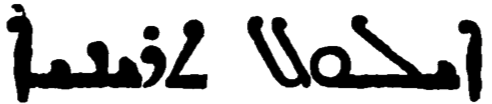
\includegraphics[height=10pt]{tables/099/13} } &
 Elul alter. &
 \textgreek{γορπιαῖος δευτερος.[?]} &
 5
\\
\bottomrule
\end{tabular}
%
\end{table}
%
% 99
% {PDF page nr}{source page nr}{line nr}
\plnr{182}{99}{4}Et Syromacedonas quidem utroque anno, aequabili
scilicet et mere Graeco, item Lunari usos fuisse, exemplo Atheniensium,
Macedonum, et reliquorum Graecorum, qui duplici anno
utebantur, ut diximus, vulgus quidem populari aequabili, magistratus
vero Lunari, quem Attici \textgreek{ἔτος κατὰ σελήνην[?]},
 item \textgreek{ἔτος πρυτανείας[?]}
vocabant.
\lnr{9}Sed Chaldaeos usos non dubito unico tantum Lunari,
ut fecerunt etiam Iudaei, qui tum primum scriptum annum
habere caeperunt, cum antea usurparent ex observatione aut alio
modo.
\lnr{12}Utrique tamen tam Iudaei, quam Chaldaei hac periodo retenta
retinuerunt epocham anni Solaris ineuntis quidem \textgreek{ἀπὸ τοῦ κέντρου
μετοπωρινοῦ[?]}, in \rnum{vii} Octobris, definentis vero in \rnum{vi}.
\lnr{14}Itaque eandem
epocham hactenus retinent Iudaei, ut sequenti capite dicetur.
\lnr{16}Nunc periclitemur sidem periodi Chaldaicae, ex iis, quae legimus
apud Ptolemaeum.
\lnr{17}Anno Nabonassari 512, Thoth \rnum{ix}, Chaldaeorum
vero 75, \textgreek{δίου[?] \gnum{ιδ}},
 Sol deprehensus in 5.10' Scorpii.
\lnr{18}Tempus, annus
periodi Iulianae 4477, Octobris 29, feria quinta, cyclo Solis 25.
\lnr{20}Ergo neomenia Dii fuit feria sexta.
\lnr{20}Annus 75 Chaldaeorum, ut iam
didicisti, est 76, et ultimus periodi primae Syromacedonum.
\lnr{21}Hyperberetaeus 16 Septembris, feria quarta.
\lnr{22}Ergo in Tabula periodi e regione
76 anni 4 composita cum charactere \textgreek{Δίου[?]}~2, posito in Tabula
mensium dabit feriam \rnum{vi}, ut propositum fuit cui cunvenit Marcheswan
%% Note: The body text writes "Marcheſvvan", while the page linker
%% writes "Marcheſwan". This indicates that the "w" (double-u) used in this
%% text and e.g. in the table on page 99 (where it stands out as a character
%% from another, slightly higher, font) indeed represents a double-v ("vv").
Iudaicus anni 3525.
%
% 100
% {PDF page nr}{source page nr}{line nr}
\plnr{183}{100}{1}Cuius character 6.5.375.
\lnr{1}Rursus anno Nabonassari
519, Tybi 14, Chaldaeorum vero 82,
 \textgreek{ξανθικοῦ[?] \gnum{ε}}, Sol obtinebat
6.10' Piscium.
\lnr{3}Tempus annus periodi Iulianae % looks like written as "e-with-cedille"
 4485, Kalendae
Martiae, % again e-with-cedille
 feria quarta.
\lnr{4}Ergo neomenia Xanthici fuit feria septima.
\lnr{4}Annus
82, abiectis 76, est sextus secundae periodi Chaldaicae, et proinde
septimus secundae Syromacedonicae.
\lnr{6}Hyperberetaeus 31 Augusti, feria
tertia, cyclo Solis \rnum{iiii}.
\lnr{7}Quae composita cum regulari Xanthici 2 in
Tabula mensium, dabit feriam quintam in neomenia Xanthici.
\lnr{8}Erratum
igitur biduo: et proinde apud Ptolemaeum legendum \textgreek{Ξανθικοῦ[?]} Z,
non autem \textgreek{Ξανθικοῦ[?]} E.
\lnr{10}De quo dubitari non debet.
\lnr{10}Conveniet etiam
cum Adar gemino anni 3532: cuius character 5.12.178.
\lnr{11}Postremo anno
Nabonassari 504, Thoth 27, secundum Chaldaeos 67, \textgreek{ἀπελλαίου[?]
 \gnum{ε}}, Sol erat in 24.50' Scorpii.
\lnr{13}Tempus annus periodi Iulianae 4469,
Novembris 18, feria prima, cyclo Solis 17.
\lnr{14}Ergo neomenia Apellaei 14
Novembris, feria quarta.
\lnr{15}Hyperberetaeus autem anni 68 Syromacedonici
15 Septembris feria septima.
\lnr{16}Ergo neomenia Apellaei feria tertia,
not quarta: cui convenit character Casleu anni 3517.
\lnr{17}Fuit enim 3.5.421.
\lnr{18}Itaque error est in Codice Ptolemaei,
 \textgreek{\gnum{ε}} pro \textgreek{\gnum{ϛ}}.
\lnr{18}Hactenus quae habuimus
de anno Chaldaico.
\lnr{19}Quod autem apud Censorinum de Chaldaica
Dodecaeteride scriptum extat, quanuis ad hanc rem nihil pertinet,
tamen, quia res scitu dignissima visa est, eam nolui praeterire.
\lnr{22}Verba Censorini:
\textit{Proxime hanc magnitudinem, quae vocatur Dodecaeteris,
ex annis vertentibus duodecim.}
\lnr{23}\textit{Huic anno Chaldaico nomen est: quem
Genethliaci non ad Solis Lunaeque cursus, sed ad observationes alias habent 
accommodatum: quod in eo dicunt tempestates frugumque proventus,
ac sterilitates, item morbos salubritatesque circumire.}
\lnr{26}Haec % e-cedille
 vetus scriptor
Censorinus.
\lnr{27}Intelligit autem Dodecateririda, quam etiamnum retinent
Chaldaei, Persae, Sinae, % e-cedille
 Indi, Chataii, Turcae, Syri, Arabes, Totari,
sive Tartari.
\lnr{29}Ea vocatur \textarabic{[Arabic]} Schaichun.
% Hebrew in 1593, page 78, line 9
\lnr{29}Putant re vera sterilitates,
morbos, proventus cum ea redire, ut scripsit Censorinus. % 1629: "Censorin."
\lnr{30}Ideo singulos
annos Dodecaeteridis animalium nominibus appellant, quae affectum
eius anni indicent.
\lnr{32}Puta annum pestilentem vocant annum Serpentis.
\lnr{32}Annum
fertilitatis, Leporem.
\lnr{33}Annum bellicorum tumultuum, Equum.
\lnr{33}Annum
felicis agricolationis, Taurum.
\lnr{34}Annum famis, Murem.
\lnr{34}Non solum
autem Censorinus % 1629: "Censor.". From 1598 edition p78: Censorinus
 declarat Genethliacorum propriam fuisse dodecaeterida,
sed etiam Marcus Polus Ventus liber \rnum{ii} caput \rnum{xxv}
% 1629: "l.2.c.25".
\lnr{36}Sciendum vero
aeram Tartarorum per Dodecaeteridas procedere.
\lnr{37}Primus annus Leonis
titulo notatur; secundus Bovis: tertius Draconis; quartus Canis; et
ita deinceps, donec duodecim anni explicentur.
\lnr{39}Quare aliquis interrogatus
ab % à -> ab
 Genethliaco de anno natali, respondet se natum, verbi gratia
anno Leonis, illa die, nocte, et hora, et momento.
\lnr{41}Idque diligenter
a patribus notatur edito in lucem puero, et in libro aliquo scribitur.
%
% 101
% {PDF page nr}{source page nr}{line nr}
\plnr{184}{101}{2}Explicito animali duodecimo, hoc est, anno duodecimo,
 rursus ad
primum signum, hoc est, Leonem reditur.
\lnr{3}Haec diserte Polus Venetus.
\lnr{4}Ex quibus non solum docetur usus Dodecaeteridos, sed etiam apparet
non per omnia illas nationes in nominibus animalium convenire.
\lnr{6}Nam Bos sive Taurus, est quidem secundus annus tam in Tartarica,
quam in nostra Dodecaeteride.
\lnr{7}Sed Draco est tertius Tartaricae, cum
sit quintus nostrae.
\lnr{8}Canis est penultimus nostrae, et quartus Tartaricae.
\lnr{9}Leo vero est primus Tartaricae, qui in nostra nusquam locum habet.
\lnr{10}Ignatius Patriarcha Antiochenus, vir perfectissimus, neque enim aliter
eum vocare possum, cum fuerit doctrinae, virtutumque omnium
absolutissimum exemplar, is igitur summus vir ad me scribens anno
Christi 1581, monebat eum annum esse sextum illius Dodecaeteridis,
et cognominem Serpentis.
\lnr{14}Adducerem etiam eius verba, nisi vererer
ea deterere culpa ingenii.
\lnr{15}Neque enim Latine assequar, quae ille elegantissime
idiomate suo Arabico prosectus est.
\lnr{16}Subiiciam tamen
Diagramma illius periodi dodecaetericae, quinque linguis primum ab
illo perscriptum, et Latine a nobis deinde redditum. % 1593 p78: "à".
%
% Table p101: Nomina annorum Schaichun sive dodecaeteridos Chaldaicae
\begin{table}[tb]
  %%% Liber II p101, PDF 184
%%
%% Table in the section "De periodo Chaldaeorum Alexandrea"
%% Title is given in the original.
%% The body of the table is filled mostly with Arabic, Turkish, Persian and
%% "Chatai", which all look arabic. There is also a column of Syrian,
%% same as what is seen in the table on p99.
%%
%% In the 1593 edition, p78, the body of this table is filled with Hebrew,
%% and the column of numbers is headed "Anni Schaichun."
%%
%% There is currently (nov 2017) no information on the Chaldean calendar
%% on Wikipedia
%%
%%% Count out columns for fixed-width source font
% 000000011111111112222222222333333333344444444445555555555666666666677777777778
% 345678901234567890123456789012345678901234567890123456789012345678901234567890
%
%% Select a general font size (uncomment one from the list)
%\tiny
%\scriptsize
%\footnotesize
%\small
\normalsize
%
%% Center the whole table left-right
\centering
%
%% Modify separation between columns
%\setlength{\tabcolsep}{1.6pt}
%
%% Modify distance between rows
%\renewcommand{\arraystretch}{1.3}
%%
\begin{tabular}{@{}l c r r r r r@{}}
\toprule
 \multicolumn{7}{c}{\Large\textsc{Nomina annorum Schaichun}}\\
 \multicolumn{7}{c}{\large\textsc{sive dodecaeteidos Chaldaicae}}
\\
\toprule
 \multicolumn{6}{c}{~} &
 \multicolumn{1}{c}{Chatai}
\\
 \multicolumn{1}{l}{Latini} &
 &
 \multicolumn{1}{c}{Syri} &
 \multicolumn{1}{c}{Arabes} &
 \multicolumn{1}{c}{Turcae} &
 \multicolumn{1}{c}{Persae} &
 \multicolumn{1}{c}{\& Ieguraei}
\\
\midrule
 \textsc{mus} &
 \rnum{i} &
 [?] &
 \textarabic{شيخون}[?] &
 \textarabic{شيخون}[?] &
 \textarabic{شيخون}[?] &
 \textarabic{شيخون}[?]
\\
 \textsc{taurus} &
 \rnum{ii} &
 [?] &
 \textarabic{شيخون}[?] &
 \textarabic{شيخون}[?] &
 \textarabic{شيخون}[?] &
 \textarabic{شيخون}[?]
\\
 \textsc{pardus} &
 \rnum{iii} &
 [?] &
 \textarabic{شيخون}[?] &
 \textarabic{شيخون}[?] &
 \textarabic{شيخون}[?] &
 \textarabic{شيخون}[?]
\\
\midrule
 \textsc{lepus} &
 \rnum{iiii} &
 [?] &
 \textarabic{شيخون}[?] &
 \textarabic{شيخون}[?] &
 \textarabic{شيخون}[?] &
 \textarabic{شيخون}[?]
\\
 \textsc{draco} &
 \rnum{v} &
 [?] &
 \textarabic{شيخون}[?] &
 \textarabic{شيخون}[?] &
 \textarabic{شيخون}[?] &
 \textarabic{شيخون}[?]
\\
 \textsc{serpens} &
 \rnum{vi} &
 [?] &
 \textarabic{شيخون}[?] &
 \textarabic{شيخون}[?] &
 \textarabic{شيخون}[?] &
 \textarabic{شيخون}[?]
\\
\midrule
 \textsc{equus} &
 \rnum{vii} &
 [?] &
 \textarabic{شيخون}[?] &
 \textarabic{شيخون}[?] &
 \textarabic{شيخون}[?] &
 \textarabic{شيخون}[?]
\\
 \textsc{ovis} &
 \rnum{viii} &
 [?] &
 \textarabic{شيخون}[?] &
 \textarabic{شيخون}[?] &
 \textarabic{شيخون}[?] &
 \textarabic{شيخون}[?]
\\
 \textsc{simia} &
 \rnum{ix} &
 [?] &
 \textarabic{شيخون}[?] &
 \textarabic{شيخون}[?] &
 \textarabic{شيخون}[?] &
 \textarabic{شيخون}[?]
\\
\midrule
 \textsc{gallina} &
 \rnum{x} &
 [?] &
 \textarabic{شيخون}[?] &
 \textarabic{شيخون}[?] &
 \textarabic{شيخون}[?] &
 \textarabic{شيخون}[?]
\\
 \textsc{canis} &
 \rnum{xi} &
 [?] &
 \textarabic{شيخون}[?] &
 \textarabic{شيخون}[?] &
 \textarabic{شيخون}[?] &
 \textarabic{شيخون}[?]
\\
 \textsc{porcus} &
 \rnum{xii} &
 [?] &
 \textarabic{شيخون}[?] &
 \textarabic{شيخون}[?] &
 \textarabic{شيخون}[?] &
 \textarabic{شيخون}[?]
\\
\bottomrule
\end{tabular}
%
\caption{Nomina annorum Schaichun}
\label{tab:101}

\end{table}
%
% 102
% {PDF page nr}{source page nr}{line nr}
\plnr{185}{102}{1}Gavisi itague sumus ea quae legeramus de hac
 Dodecaeteride apud
Censorinum, Polum Venetum, et alios, per omnia conveniere descriptioni
Ignatii Patriarchae.
\lnr{3}Sed non possum me continere, quin proferam
in mendium suspicionem meam de anno Chaldaico et hac Dodecaeteride.
\lnr{5}Arbitror enim antiquos Chaldaeos primum annum
Calippicae suae periodi a primo illius Dodecaeteridis incepisse: et, nisi
me fallit coniectura, propterea distulisse computum suum in secundus,
primus fuisse Dodecaeteridos.
\lnr{9}Neque dubito, quin verum sit.
\lnr{9}Ita
annus Christi 1581, qui erat 1892 Syrorum, 1891 Chaldaeorum, erat
non sextus, sed septimus illius periodi.
\lnr{11}Et noli dubitare de hac re.
\lnr{11}Nam
certo certius Chaldaeos in Thematibus genethliacis nulla alia epocha
annorum usos, quam Syromacedonica, de qua locuti sumus.
\lnr{13}Et potest fieri annum septimum Dodecaeteridos incepisse in medio anno
Christi 1581, Ignatium autem tunc ad me scripsisse eodem anno, ante
quam sextus ad finem decurrisset.
%
%====
\section{De Periodo Iudaeorum Alexandrea}
%
\lnr{17}Dici non potest, quantum inter se velitentur veteres Magistri
Hebraeorum, cum ad illum locum Exodi \rnum{xii} pervenerunt:
Hic mensis erit vobis initium mensium.
\lnr{19}Nemo eorum est,
quotquot in illum locum scripserunt (sunt autem infiniti) qui non ansam
arripiat de veterum Hebraeorum anno disputandi.
\lnr{21}Omnium
consensus unus, Lunarem eum fuisse.
\lnr{22}Et sane verum dicunt.
\lnr{22}Sed mira
dissensio in neomeniis determinandis, cum alii ex observatione, alii ex
scripto, quod vocant \texthebrew{[Hebrew]}, indici solitas prodant.
\lnr{24}Et rursus urum
\textgreek{ἀπὸ τὴς φάσεως[?]}, an \textgreek{ἀπὸ τὴς συνόδου[?]},
 intituerentur, dubitant.
\lnr{25}In hoc opinionum bivio, quis intendet digitum?
\lnr{26}Confugiendum ad vetustiora
eius gentis monumenta.
\lnr{27}In Pandecte Digestorum Thalmudicorum,
Capite Ros haschana, omnino scriptum est, antiquitus
neomenias \textgreek{ἀπὸ τὴν φάσεως[?]} indici solitas: ad eamque rem testes et
specularotres idoneos delegatos, scelerum et vitiorum puros, non
ebriosos, non aleones, non nocturnos praemiatores: de quarum personarum
delectu longas diatribas instituunt.
\lnr{32}Cum igitur reversi renunciarent
se Lunam nascentem vidisse, tum a iudicibus succlamabatur
\texthebrew{[Hebrew]}, Sanctificata est, Sanctificata est Neomenia.
\lnr{34}Subaudiendum
enim \texthebrew{[Hebrew]}.
\lnr{35}Eoque nomine etiam hodie in Ritualibus Iudaeorum
extat carmen Lunae visae sanctificandae.
% 1598 p99: extat vetus carmen
\lnr{36}Lunam visam Arabes
vocant \textarabic{[Arabic]}, Halil: a qua omnes Mahumedani
 neomenias instituunt,
non \textgreek{ἀπὸ τὴς συνόδου[?]} vox \textarabic{[Arabic]} vel
 \textarabic{[Arabic]} est \textgreek{ἐξαυγασμὸς[?]}.
%
% 103
% {PDF page nr}{source page nr}{line nr}
\plnr{186}{103}{1}\textarabic{[Arabic]}
est \textgreek{συνόδου[?]}.
\lnr{2}Vocant etiam \textgreek{τὴν φάσιν[?]} \textarabic{[Arabic]}
\lnr{2}Renunciata Lunae visione,
(ita loquitur Vitruvius) statim neomenia tubae clangore indicebatur.
\lnr{4}Quia igitur ab observatione neomenia instituebatur, propterea non raro
accidebat, ut duo menses nunc cavi, nunc solidi, continuarentur, pro
ratione \textgreek{τὴς φθάσεως[?]},
 aut \textgreek{τὴς ὑστερήσεως τὴς φάσεως[?]}: ut non immerito propter
hanc anomalian dictum sit de Luna \texthebrew{[Hebrew]}.
\lnr{7}\textgreek{τότε
μὲν ὑπολειπομένη, τότε δὲ ὑποφθάνουσα[?]}.
\lnr{8}Hoc verisimille est locum habuisse
in vetustissimis Hebraeis, quibus adhuc ratio motus et curriculi Lunaris
ignota erat.
\lnr{10}Non enim poterant, nisi ex observatione, suas neomenias
in vulgus publicare.
\lnr{11}Sed puto hoc magis inter Iudices ipsos
quam apud populum obtinuisse, et potius Ecclesiasticas, quam politicas
neomenias fuisse.
\lnr{13}Alioqui quomodo tot millia Iudaeorum tantis
locorum intervallis diffita, in vallibus depressis, in locis Septentrionalibus,
in quibus raro nascens Luna oculis hominum potestatem
suae speciei facit propter interventum nubilorum, Lunam nascentem
intueri, aut a Iudaea nuncium exspectare potuissent?
\lnr{17}Oportet igitur
eis aliquid praescripsisse, quod sequerentur in neomenia statuenda,
cum Lunam nascentem videre aut tempestates, aut familiaria regionum
nubila impedirent.
\lnr{20}Quare concludimus, eos longe ante tempora
Messiae designatam in libris anni formam habuisse: ut et hodie non
solum ipsi Iudaei, sed etiam Samaritae habent:
 quam utrique \texthebrew{[Hebrew]} vocant,
hoc est, \textgreek{ἐμβολισμόν[?]}.
\lnr{23}Qui sit, ut Samaritani, qui ab hinc plusquam
bis mille annis nihil commune cum Iudaeis nec divini, neque humani
habent, habeant tamen idem nomen Hebraeum, quo eandem rem
notent?
\lnr{26}Sane hoc non fieret, nisi res vetustissima esset.
\lnr{26}\texthebrew{[Hebrew]} igitur proprie
est \textgreek{ἐμβολισμός[?]}.
\lnr{27}Sed, ut dixi, anni ratio in libros redacta et scripto
concepta, ita ab utraque natione vocatur.
\lnr{28}Cui rei etiam fidem facit,
quod in eodem capite Rosch haschana scriptum extat, Iudices, cum
de neomenia speculatum homines delegarent,
 ipsos inante \texthebrew{[Hebrew]}
habuisse, id est figuram Lunae, quod intelligo
 \textgreek{ψηφοφορίαν σεληνιακῶν
συνόδων[?]};
ad quam nimirum confugerent, quoties nubila, aut imbres
visionem Lunae oculis inviderent.
\lnr{33}Sane magna me huius rei incessit
admiratio, quomodo hoc fieri posset omni tempore.
\lnr{34}Nam Luna
pauculis horis a coitu videri potest, quanquam raro, idque potius cum
est in Ariete quam alias.
\lnr{36}Sequentis neomeniae \textgreek{φάσις[?]} saepenumero secundo
die a coitu apperebit.
\lnr{37}Ita mensis instituendus foret unius et
triginta dierum.
\lnr{38}Quod est absurdum in anno Lunari.
\lnr{38}Sed textus Thalmud
eodem capite dicit, ubi tricesima prima nocte Luna se videndam
negaret, tunc neomeniam definiri solitam.
\lnr{40}Quod sane alias computus
ex scripto promittere poterat.
\lnr{41}Igitur \texthebrew{[Hebrew]}, hoc est collegium vel
consistorium iudicum solum neomenius indicendi ius habebat: ad
quod etiam pertinebat ius \textgreek{ἐμβολισμοῦ[?]},
 hoc est, menses intercalandi.
%
% 104
% {PDF page nr}{source page nr}{line nr}
\plnr{187}{104}{3}Quamius enim status ex scripto esset situs embolismi,
 tamen propter
quasdam caussas insuper habebatur.
\lnr{4}Ut nos docuit summus Magister
Moses filius Maimon in sua Iad, capite in Kiddusch Haccodesch:
\texthebrew{[Hebrew]}.
\lnr{6}Propter
tres casus intercalabant in anno, propter epocham anni solaris,
propter fruges maturas, et propter fructus arborum.
\lnr{8}Subiicit:
\texthebrew{[Hebrew][multiple lines]}.
\lnr{12}Si iudices animadvertissent nondum
maturas esse fruges, sed adhuc ferotinas esse, neque fructus arborum,
quibus mos est tempore Paschali florere: illis duobus argumentis nitebantur,
et intercalabant in anno.
\lnr{15}Ac quanquam epocha anni antevertebat
sextam decimam mensis Nisan, tamen intercalabant, ut
frumentum maturum esset, ex quo offerretur manipulus in \rnum{xvi}
Nisan, et ut fructus florerent more omnium.
\lnr{18}Sed ad hanc rem
faciebat epistolium a Iudicibus ad Galilaeos et Transiordanianos
missum, quod cum multis aliis vetustatis monumentis in hanc materiam
congesseramus.
\lnr{21}Quae omnia in Gallia reliquimus.
\lnr{21}Neque nobiscum
huc ulla studiorum praesidia attulimus.
\lnr{22}In illa epistola redditur
ratio, quare ex Nisan Adar secundum facere deberent: nimirum propter
fruges nondum maturas, et eas caussas, quas supra adduximus.
\lnr{25}Pene iisdem verbis reperias apud eundem Mosem:
 \texthebrew{[Hebrew][many lines]}.
\lnr{28}Iudices computo inito sciebant si Tekupha Nisan esset in sextadecima
Nisan, aut post: et intercalabant in eo anno, mutato Nisan in
Adar geminum, nimirum ut Pesach incideret in tempus frugum maturarum:
et cum huic signo inniterentur, ita intercalabant, neque
alius ullius signi rationem habebant.
\lnr{32}Eadem haec omnia reperies in
Thalmud.
\lnr{33}Ex quibus manifestum est, fieri posse, ut duo anni deinceps
intercalarentur: quod in Thalmud de Rabbi Akiba scriptum legimus,
qui duos continuos annos intercalavit.
\lnr{35}Nam supra dictum est,
etiam si sextadecima Nisan pervenisset ad Tekupham, tamen intercalari
solitum.
\lnr{37}Si Tekupha Nisan erat in \rnum{viii} Aprilis; cum cyclus esset
\rnum{ix}, eo anno Tekupha incidebat in Pascha, et tamen ille mensis
vocabatur Adar posterior, et Nisan incipiebat in 23, aut 24 Aprilis.
\lnr{40}Sed paragrapho tertio adducuntur aliae necessitates intercalandi,
propter \textgreek{ἐπιχειμασίαν[?]}, propter tempestates, propter pontes eversos,
propter diluvia, et pluvias, quando scilicet populus Hierosolyma
convenire non poterat: item propter fornaces, quae agno assando construebantur,
dirutas: et propter alia, quae prudens linquo iis, quod illa
ex Mose filio Maimon, aut ex Thalmud petere possunt in capite Pesach.
%
% 105
% {PDF page nr}{source page nr}{line nr}
\plnr{188}{105}{4}Iudaei igitur simul cum iugo
 Seleucidarum eorum annum et epocham
acceperunt, non tamen \textgreek{ἀπὸ τὴς φάσεως[?]},
 ut hodie Hagareni, et ut ipsimet
Iudaei saepe antea potuerunt facere, ex observatione
 \textgreek{τὴς φάσεως, καὶ τοῦ φεγγαρίου[?]},
sed \textgreek{ἀπὸ τῆς συνόδου[?]}: ut habes supra in periodo Syromacedonum.
\lnr{8}Est enim eadem periodus Syromacedonica, Chaldaica, Iudaica, ut diximus:
cui additae sunt \textgreek{περιτταὶ ἡμέραι[?]}, ut sciatur intervallum, quod est
a neomenia Tisri, ad \textgreek{κέντρον μετοπωρινὸν[?]},
 id est, Tekupham, nempe ad 7
Octobris, quod erat principium periodi Seleucidarum, sive Syromacedonum,
ut toties demonstratum
est.
%
% Table: Tabula characterismi mensium Iudaicorum
\begin{table}[t]
  \centering
  %%% Liber II p101, PDF 184
%%
%% Table in the section "De periodo Chaldaeorum Alexandrea"
%% Title is given in the original.
%% The body of the table is filled mostly with Arabic, Turkish, Persian and
%% "Chatai", which all look arabic. There is also a column of Syrian,
%% same as what is seen in the table on p99.
%%
%% In the 1593 edition, p78, the body of this table is filled with Hebrew,
%% and the column of numbers is headed "Anni Schaichun."
%%
%% There is currently (nov 2017) no information on the Chaldean calendar
%% on Wikipedia
%%
%%% Count out columns for fixed-width source font
% 000000011111111112222222222333333333344444444445555555555666666666677777777778
% 345678901234567890123456789012345678901234567890123456789012345678901234567890
%
%% Select a general font size (uncomment one from the list)
%\tiny
%\scriptsize
%\footnotesize
%\small
\normalsize
%
%% Center the whole table left-right
\centering
%
%% Modify separation between columns
%\setlength{\tabcolsep}{1.6pt}
%
%% Modify distance between rows
%\renewcommand{\arraystretch}{1.3}
%%
\begin{tabular}{@{}l c c c c c c@{}}
\toprule
 \multicolumn{7}{c}{\Large\textsc{Tabula characterismi}}\\
 \multicolumn{7}{c}{\large\textsc{mensium Iudaicorum}}
\\
\toprule
 
 ~ &
 \multicolumn{3}{c}{Communis} &
 \multicolumn{3}{c}{Embolimaeus}
\\
\cmidrule(lr){2-4}
\cmidrule(lr){5-7} 
 ~ &
 \multicolumn{1}{c}{\scriptsize Defectivus} &
 \multicolumn{1}{c}{\scriptsize Ordinarius} &
 \multicolumn{1}{c}{\scriptsize Abundans} &
 \multicolumn{1}{c}{\scriptsize Defectivus} &
 \multicolumn{1}{c}{\scriptsize Ordinarius} &
 \multicolumn{1}{c}{\scriptsize Abundans}
\\
\midrule
 \textsc{Tisri} &
 0 &
 0 &
 0 &
 0 &
 0 &
 0
 \\
 \textsc{Marcheswan} &
 2 &
 2 &
 2 &
 2 &
 2 &
 2
\\
 \textsc{Chaslev} &
 3 &
 3 &
 4 &
 3 &
 3 &
 4
\\
\midrule
 \textsc{Tebeth} &
 4 &
 5 &
 6 &
 4 &
 5 &
 6
\\
 \textsc{Schebat} &
 5 &
 6 &
 7 &
 5 &
 6 &
 7
\\
 \textsc{Adar prior.} &
 0 &
 0 &
 0 &
 7 &
 1 &
 2
\\
 \textsc{Adar poste.} &
 7 &
 1 &
 2 &
 2 &
 3 &
 4
\\
\midrule
 \textsc{Nisan} &
 1 &
 2 &
 3 &
 3 &
 4 &
 5
\\
 \textsc{Iiar} &
 3 &
 4 &
 5 &
 5 &
 6 &
 7
\\
 \textsc{Siwan} &
 4 &
 5 &
 6 &
 6 &
 7 &
 1
\\
\midrule
 \textsc{Thamuz} &
 6 &
 7 &
 1 &
 1 &
 2 &
 3
\\
 \textsc{Ab} &
 7 &
 1 &
 2 &
 2 &
 3 &
 4
\\
 \textsc{Elul} &
 2 &
 3 &
 4 &
 4 &
 5 &
 6
\\
\bottomrule
\end{tabular}
%
\end{table}
%
\lnr{13}Nam quatuor quadrantum
diei maximam rationem
habebant Iudaei; habentque
hodie, ut suo loco ostendetur
in Computo Iudaico.
\lnr{18}Quare Tekupha Tisri erat in
septima Octobris: Tekupha
Tebeth in septima Ianuarii:
Tekupha Nisan in octava Aprilis:
Tekupha Thamuz in octava
Iulii: omnes in litera G.
\lnr{24}Praeterea adiecimus hic laterculum
characterismi mensium
Iudaicorum tam in anno communi,
quam embolimaeo.
\lnr{27}Sed in utraque differentia anni sunt ternae
praeterea differentiae.
\lnr{28}Nam annus, sive communis sit, sive embolimaeus,
est aut ordinarius, aut abundans, aut defectivus.
\lnr{29}Ordinarius communis
354 dierum, embolimaeus 384.
\lnr{30}Abundans et defectivus vocantur,
prout unus dies accessit, aut decessit.
\lnr{31}Sedes autem \textgreek{ἐξαιρέσεως[?]} est semper
in Caslevv.
\lnr{32}Nam cum Caslevv sit ordinarie plenus, extra ordinem sic
cavus, et locus \textgreek{προσθέσεως[?]} est in Marchesvvan,
 qui ordinate est cavus,
extra ordinem plenus.
\lnr{34}Differentiae hae nascuntur ex superstitione characterismorum
Tisri et Nisan.
\lnr{35}Nam characterismus Tisri nunquam
potest esse aut feria prima, aut quarta, aut sexta.
\lnr{36}Characterismus Nisan
nunquam potest esse feria secunda, neque quarta, neque sexta.
\lnr{37}Hinc
colligitur tantum hos characterismos competere neomeniae quidem
Tisri, ferias 2, 3, 5, 7: Neomeniae Nisan, 1, 3, 5, 7.
\lnr{39}Hinc rursus colligitur,
cum character Tisri est feria quinta, nunquam annum communem
esse defectivum, nunquam Embolimaeum ordinarium.
\lnr{41}Cum est feria
tertia, neque communis, neque Embolimaeus unquam est defectivus,
neque communis unquam abundans.
%
% 106
% {PDF page nr}{source page nr}{line nr}
\plnr{189}{106}{2}Cum feria est secunda, nunquam
communis aut embolimaeus est ordinarius, ut neque cum feria
est septima.
\lnr{4}Alioqui Nisan incurreret in ferias, 2, 4, 6.
\lnr{4}Haec periodus
quam proposuimus, cum loqueremur de anno Syromacedonico, non
solum utilis est ad annos Iudaicos notandos, sed etiam sine illa nunquam
illos deprehendere poteris.
\lnr{7}Hac Iudaei usque ad tempora Constantini
Magni et infra illa tempora usi sunt, cum iam Luna biduum
veterem epocham antevertisset.
\lnr{9}Et hanc quidem epochen vocant
aeram contractuum, vel \texthebrew{[Hebrew]}.
\lnr{10}Nunc tempus est, ut eius sidem periclitemur.
\lnr{11}Primum igitur de translatione characterismi Tisri, quod
quidam Rabbini dicunt post Thalmuldis editionem excogitatum esse,
et quidam ex nostris sibi persuaserunt, omnino utrosque ratio fugit.
\lnr{14}Antiquitus enim et sub Seleucidis usurpatum.
\lnr{14}Anno passionis Dominicae
Neomenia Nisan incidit in Sabbatum: cum tamen eius character
ex hodierno epilogismo sit 5.19.95, feria sexta.
\lnr{16}Sed id demonstrandum
ex side nostrae periodi Seleucidarum.
\lnr{17}Erat annus Contractuum,
sive Alexandreus 344: et proinde quadragismus annus periodi
quintae. % e-cedille
\lnr{19}Tisri 24 Septembris, feria quarta: quae mutata in quintam
in anno communi ordinario dat feriam septimam neomeniae Nisan.
\lnr{21}Rursus anno Christi vulgari 70 neomenia Nisan fuit Kal. % Abriv.
 Aprilis, teste
Iosepho.
\lnr{22}Nam quartadecima Nisan conveniebat cum quartadecima
mensis Iuliani.
\lnr{23}Erat annus primus sextae periodi Contractuum, Tisri
6 Septemb. % Abriv.
 feria quarta, cyclo Solis 22.
\lnr{24}Ergo mutata in quintam
cum characterismo feriae Nisan composita in anno Embolimaeo defectivo
dabit feriam primam Neomeniae Nisan in Kal. % Abriv.
 Aprilis, Cyclo
Solis 23.
\lnr{27}In utroque igitur exemplo translatio feriae fuit politica.
\lnr{27}Imo
nunquam ex epilogismo hodierno illam neomeniam reperire possis.
\lnr{29}Nam ut Iudaei hodie putant, fuerit Neomeniae Nisan characterismus
6.19.409, Sabbato, ultima Martii.
\lnr{30}Quo epilogismo si usi fuissent illis
temporibus, neomenia Nisan, ut vides, fuisseet in feria septima, non, ut
Iosephus vere scribit, in feria prima.
\lnr{32}Sed et fidem huius excellentissimae
periodi pluribus argumentis muniamus.
\lnr{33}Iosephus scribit, ante
initia belli Iudaici, hoc est, circa annum Christi vulgarem 67 plus minus,
multa portenta visa: inter quae narrat de fanatico quodam mira;
quae ex illo petas licet: idque accidisse, quo tempore Pascha, hoc est,
quartadecima Nisan, conveniebat cum 8 Aprilis.
\lnr{37}Hoc non potuit accidere,
nisi cum cyclus Lunae esset 9, anno Christi 65, biennio ante initia
belli Iudaici.
\lnr{39}Quod mirisice menti Iosephi convenit.
\lnr{39}Erat annus
contractuum 376.
\lnr{40}Et consequenter 72 periodi.
\lnr{40}Tisri Kalend. % Abriv.
 Septembris,
Sabbato, cyclo Solis 17.
\lnr{41}Quare Neomenia Nisan in anno embolimaeo,
feria tertia, Martii \rnum{xxvi} at \textgreek{ἡ πρώτη τῶν ἀζύμων[?]}
 \rnum{viii} Aprilis,
vel Xanthici Iuliani, ut propositum est apud Iosephum.
%
% 107
% {PDF page nr}{source page nr}{line nr}
\plnr{190}{107}{2}Hoc etiam
convenit epilogismo hodierno.
\lnr{3}Nam character Nisan fuisset 2,21.723,
feria tertia, ut iam dictum est, anno Iudaico vulgari 3825.
\lnr{4}Vides,
quam certa sit fides methodi.
\lnr{5}Sed nihil agimus, nisi porro confirmemus.
\lnr{6}Idem Iosephus ait M. Tullio Cicerone, C. Antonio \textsc{coss}.
\lnr{7}Hierosolyma capta a Pompeio fuisse \textgreek{ἐν τῇ νηστείᾳ[?]},
 hoc est \rnum{xvii} Thamuz.
\lnr{8}Dion narrans hunc casum ait eam diem Sabbatum fuisse:
neque more Gentium quoduis solenne Iudaicum Sabbatum vocat:
sed adeo Sabbatum fuisse dicit, ut hinc disputandi occasionem aucupet,
quare a Planetis nomina diebus indita sint.
\lnr{11}Tempus a Iosepho
designatur, cum ait vicesimum septimum annum fuisse ante consulatum
M. Vipsanii Agrippae, et L. Caninii Galli.
\lnr{13}Illud par Consulum
confertur in annum nonum Iulianum.
\lnr{14}Fuit ergo cyclus Lunae
tertius.
\lnr{15}Sed falsum est, interfuisse \rnum{xxvii} annos a captis Hierosolymis
a Pompeio, ad eadem a Sosio capta.
\lnr{16}Uno enim anno plus dicit,
cum vicesimum septimum annum pro viginti sex annis dicit: ut contra
Gregorius Turonensis semper dicit vicesimum sextum annnum,
pro eo qui vicesimus septimus erat.
\lnr{19}Annus captorum Hierosolymorum
a Pompeio in periodo Iuliana 4651.
\lnr{20}Rursus annus captorum
Hierosolymorum a Sosio 4677.
\lnr{21}Differentia, anni \rnum{xxvi} solido, non
utique \rnum{xxvii}, ut voluit Iosephus.
\lnr{22}Erat annus \rnum{xxi} periodi quartae
Contractuum, ordinarius communis.
\lnr{23}Tisri \rnum{xxvi} Septembris, feria
\rnum{v}, cyclo Solis \rnum{ii}.
\lnr{24}Quae quidem feria cum charactere Thamuz coniuncta
dat feriam quintam.
\lnr{25}Ergo \rnum{xvii} fuit Sabbatum, ut voluit Dio.
\lnr{25}Sed quid
magis periodo nostrae favet, quam exemplum apud Iosephum illustre
sane, et quod sine piaculo praeteriri non potest?
\lnr{27}Refert igitur ille optimus
scriptor ex Nicolao Damasceno, ea, quae contigerunt Iudaeis et
eorum Ethnarchae Hyrcano, initio imperii Antiochi eius,
 qui \textgreek{σιδήτης[?]}
dictus est.
\lnr{30}Antiochus igitur \textgreek{σιδήτης[?]} obsedit Hyrcanum, anno primo
eius sacerdotii.
\lnr{31}Foedus deinde icit cum eo post \textgreek{σκηνοπηγίαν[?]}.
\lnr{31}Hyrcanus
sectus est Regem Antiochum in expeditionem in Parthos.
\lnr{32}Forte incidit
festum Iudaicum, quo Hyrcano obiecta est religio iter facere.
\lnr{34}Adit Regem: contendit ab eo,
 ne eo die expeditio suscipiatur, aut exeatur:
quod sibi homini Iudaeo non liceret patrio festo aliquid sacere, aut
iter suscipere.
\lnr{36}Iudaeorum enim \textgreek{ἑορτὰς ἀνεκδημήτους, καὶ ἀνεξοδεύτους εἶναι[?]}.
\lnr{37}Impetrat a Rege.
\lnr{37}Verba Damasceni: \textgreek{τρόπαιον δὲ στήσας Αντίοχος ἐπὶ τῷ
Λύκῳ ποταμῷ, νικήσας Ινδάθην τὸν Πάρθων στρατηγὸν, αὐτόθι ἔμεινεν ἡμέρας
δύο, δεηθέντος Υρκανοῦ τοῦ Ιουδαίου, διά τινα ἑορτὴν πάτριον, ἐν ᾗ τοῖς Ιουδαίοις
οὐκ ἦν νόμιμον ἐηοδεύειν[?]}.
\lnr{40}Ecco duo continua solennia, aut saltem duo
continui feriati dies, propter quos abstinetur ab opere.
\lnr{41}Iosephus interpretans
verba Damasceni subiicit: \textgreek{ταῦτα μὲν οὐ ψεύδεται λέγων[?]}.
%
% 108
% {PDF page nr}{source page nr}{line nr}
\plnr{191}{108}{1}\textgreek{ἐνέστη γὰρ
ἡ πεντηκοστὴ ἑορτὴ μετὰ τὸ σάββατον[?]}.
\lnr{2}Duo igitur festivi dies, Sabbatum et
Pentecoste.
\lnr{3}Sexta Sivvan est semper Pentecoste.
\lnr{3}Quod si Pentecoste
secuta est Sabbatum, id est, si quinta Sivvan fuit Sabbatum, ergo neomenia
Sivvan fuit feria tertia.
\lnr{5}Nunc investigandum est tempus. Hyrcanus
anno primo facerdotii sui obsessus fuit ab Antiocho statim post
caedem patris Simonis.
\lnr{7}Simon autem intersectus fuit mense Adar, anno
contractuum 177, Anno Sabbatico.
\lnr{8}Igitur 177 annus Antiochenus
erat Sabbaticus, anno Iudaico hodierno 3626.
\lnr{9}Anno autem sequente
178, Antiochus foedus inivit cum eo, solenni \textgreek{σκηνοπηγίας[?]}.
\lnr{10}Sequenti aestate, ut diximus, neomenia Sivvan incidit in feriam tertiam.
\lnr{12}Videamus, an periodus nostra hoc promittat.
\lnr{12}Annus 178 contractuum
est 26 periodi Tisri, 31 Augusti, feria 3.
\lnr{13}Erat annus embolimaeus ordinarius.
% 1598 p105: ordinarius -> communis.
\lnr{14}Ex laterculo characterismi mensium habes feriam tertiam in
neomenia Sivvan.
\lnr{15}Quod erat propositum.
\lnr{15}\textgreek{ψηφοφορία[?]} hodierna Iudaica
hoc praestare non posset post annos Christi, quia una periodus Hipparchea
a Seleucidarum epocha iam praeterierat, et Luna in anteriora
unum diem solidum enisa erat.
\lnr{18}Quid opus est pluribus hanc periodum
commendare?
\lnr{19}Iam tuto potest Lector omnia gesta Machabaeorum
ad suas epochas et verum diem referre, si diligenter methodum
nostram tenuerit, ac comperendinationes neomeniae Tisri observaverit.
%
%====
\section{De Periodo Hipparchi et vero anno lunari}
%
\lnr{23}Hipparchus, quem et \textgreek{ἄνδρα φιλαλήθη[?]} Ptolemaeus,
 et Plinius
consiliorum naturae participem vocant, non solum multa emendavit
in motuum coelestium doctrina, sed etiam ex Chaldaicis
observationibus et Calippicis rationibus, cum veris et mediis syzygiis
collatis, primus ex Graecis deprehendit \textgreek{μετάπτωσιν[?]}
 cursus Lunaris intra
quatuor periodos Calippicas fieri.
\lnr{28}Quod illi facile fuit, cum eo tempore
menses Calippici in usu essent.
\lnr{29}Observavit enim non raro
Lunam duobus trientibus diei saeculo suo priscas Calippi neomenias
antevertere.
\lnr{31}Vixit autem ille, et floruit etiam post \rnum{cc} annum
Calippi.
\lnr{32}Unde si intra \rnum{cc} annos \textgreek{μετάπτωσις[?]}
 duorum trientium fieri
solet, in \rnum{ccc} igitur fiet unius solidi diei.
\lnr{33}Quatuor autem periodi Calippicae
\rnum{ccciiii} annis explicantur.
\lnr{34}Quare si intra illud intervallum
quatuor periodorum \textgreek{παράλλαξις[?]} sit,
 resoluendum erit illam quantitatem
temporis in tot syzygias, quot constant \rnum{xvi} cycli
 \textgreek{ἐννεαδεκαετηρικοὶ[?]},
qui constituunt quatuor periodos Calippicas.
\lnr{37}Quatuor periodi Calippicae
funt dierum 111036.
%
% 109
% {PDF page nr}{source page nr}{line nr}
\plnr{192}{109}{1}Quos dies, uno minus, si distribueris in
3760 syzygias, fiet una syzygia dierum 29~\myfrac{399}{752}.
\lnr{2}Quae sunt, praeter dies
29, scrupula diei plusquam 31'.51''.42'''.7'''' hoc est, horae 12.44'.41''.6'''.
\lnr{4}Cyclus autem Hipparchi erit dierum 6939~\myfrac{11}{16}.
\lnr{4}Comparatione
igitur cyclorum \rnum{xvi} Metonis, Calippi et Hipparchi facta, non magnus
labor est differentiam eorum  constituere.
%
% Table p109
\begin{table}[t]
  %%% Liber II p109, PDF 192
%%
%% Table in the section "De periodo Hipparchi et vero anno lunari"
%% No title is given in the original.
%%
%%% Count out columns for fixed-width source font
% 000000011111111112222222222333333333344444444445555555555666666666677777777778
% 345678901234567890123456789012345678901234567890123456789012345678901234567890
%
%% Select a general font size (uncomment one from the list)
%\tiny
%\scriptsize
%\footnotesize
%\small
\normalsize
%
%% Center the whole table left-right
\centering
%
%% Modify separation between columns
%\setlength{\tabcolsep}{1.6pt}
%
%% Modify distance between rows
%\renewcommand{\arraystretch}{1.3}
%%
\begin{tabular}{@{}r r r r r @{}}
\toprule
 \multicolumn{2}{c}{Cycli Hyparchi} &
 \multicolumn{2}{c}{Cycli Calippi} &
 \multicolumn{1}{c}{Cycli Metonis}
\\
\cmidrule(lr){1-2}
\cmidrule(lr){3-4}
\cmidrule(lr){5-5}
 \multicolumn{1}{c}{\scriptsize Dies collecti} &
 \multicolumn{1}{c}{\scriptsize Scrupula} &
 \multicolumn{1}{c}{\scriptsize Dies collecti} &
 \multicolumn{1}{c}{\scriptsize Scrupula} &
 \multicolumn{1}{c}{\scriptsize Dies collecti} 
\\
 ~ & 16
\\
\midrule
 6939 &
 11 &
 6939 &
 45 &
 6940
\\
 13879 &
 6 &
 13879 &
 30 &
 13880
\\
 20819 &
 1 &
 20819 &
 15 &
 20820
\\
 27758 &
 12 &
 27759 &
 0 &
 27760
\\
\midrule
 34698 &
 7 &
 34698 &
 45 &
 34700
\\
 41638 &
 2 &
 41638 &
 30 &
 41640
\\
 41577 &
 13 &
 48578 &
 15 &
 48580
\\
 55517 &
 8 &
 55518 &
 0 &
 55320
\\
\midrule
 62457 &
 3 &
 62457 &
 45 &
 62460
\\
 69396 &
 14 &
 69397 &
 30 &
 69400
\\
 76336 &
 9 &
 76337 &
 15 &
 76340
\\
 83276 &
 4 &
 83277 &
 0 &
 83280
\\
\midrule
 90215 &
 15 &
 90216 &
 45 &
 90220
\\
 97155 &
 10 &
 97156 &
 30 &
 97160
\\
 104095 &
 5 &
 104096 &
 15 &
 104100
\\
 111035 &
 0 &
 111036 &
 0 &
 111040
\\
\bottomrule
\end{tabular}
%
\caption{Cycli Hyparchi, Calippi et Metonis}
\label{tab:p109}

\end{table}
%
\lnr{6}Scribit igitur Hipparchus
\textgreek{ἐν τῷ πὲρι ἐνιαυσίου χρόνου[?]}.
\lnr{7}\textgreek{Ημεῖς δὲ μῆνας μὲν ὅλους ἑυρίσκομεν, περιεχομένους
ἐν τοῖς ιθ´ ἔτεσιν, ὅσοις κᾀκεῖνοι[?]} (intelligit Metonem et Calippum)
\textgreek{τὸν δ᾽ ἐνιαυτὸν ἔτι καὶ τοῦ τεταρτημορίου
ἔλαττον ἐπιλαμβάνοντα μάλιστα μέρος
μιᾶς ἡμέρας[?]}.
\lnr{11}\textgreek{ὡς ἐν τοῖς \gnum{τ} ἔτεσιν ἐλλείπειν παρὰ
μὲν τὸν Μέτωνα ἡμέρασ πέντε, παρὰ δὲ
τὸν Κάλιππον ἡμέραν μίαν[?]}.
\lnr{14}Malim legere
\textgreek{ἐν \gnum{τδ} ἔτεσιν[?]},
potius quam \textgreek{ἐν \gnum{τ} ἔτεσιν[?]}.
\lnr{15}Neque aliter scripsit Hipparchus.
\lnr{15}Sed
in ratione \textgreek{μεταπτώσεως ἐνιαυσίας[?]} ipse et
Ptolemaeus contenti sunt \rnum{ccc} annis.
\lnr{18}Hoc potes ex collatione ipsa trium magnarum
periodorum colligere.
\lnr{19}Magna
periodus Hipparchi dierum 111035.
\lnr{21}Cui respondent Metonis dies 111040.
\lnr{22}Differentia \rnum{v} dies.
\lnr{22}Rursus differentia
111035 Hipparchi, et 111036 Calippi,
dies unus.
\lnr{24}Quin etiam codex Censorini
manuscriptus ait annum Metonis Solarem fuisse dierum 365, et
dierum item quinque partis undevicesimae.
\lnr{26}Quinque dies fiunt
horae 120.
\lnr{27}Resolutae in 19 dant horas 6~\myfrac{6}{19}.
\lnr{27}Duc igitur dies 365, horas
6~\myfrac{6}{19} in 304.
\lnr{28}Habebis dies 111040.
\lnr{28}Periodus igitur Hipparchae constat
quatuor periodis Calippicis, uno die minus; quemadmodum periodus
Calippica quatuor Metonicis; uno item die minus.
\lnr{30}In periodo
Calippica, praeter annos quadraginta octo communes, et 28 embolimaeos,
funt etiam, ut dixi, quindecim \textgreek{ὑπερήμεροι[?]},
 id est, quorum \textgreek{σκιῤῥοφοριὼν[?]}
est plenus, vel uterque Scirrhophorion est plenus, si est annus
embolimaeus.
\lnr{34}Annus autem ultimus, sive 76, est \textgreek{ὑπερήμερος[?]}.
\lnr{34}Igitur
cum periodus Hipparchea constet ex quatuor periodis Calippicis, debet
habere quater quindecim annos \textgreek{ὑπερημέρους[?]}.
\lnr{36}Sed ultimus annus,
hoc est trecentesimus quartus, non erit \textgreek{ὑπερήμερος[?]}.
\lnr{37}Et ita in periodo
Hipparchea sunt anni \textgreek{ὑπερήμεροι[?]} undesexaginta.
\lnr{38}Cum igitur prima
neomenia periodi Calippicae caeperit in 29 Iunii, prima neomenia
quintae periodi ascendet in 28 Iunii, quod annus ultimus quartae periodi
Calippicae non fuerit \textgreek{ὑπερήμερος[?]},
 ut in prioribus tribus, sed dierum
duntaxat 354.
%
% 110
% {PDF page nr}{source page nr}{line nr}
\plnr{193}{110}{1}Incipit autem haec nobilissima periodus anno
Nabonassari 606, neomenia Thoth, cum Tisri anni 3619 esset 6.18.601.
in ultima Epagomenon, sequente neomenia Thoth, feria sexta,
sequente septima, 28 Septembris.
\lnr{4}Aequinoctium autem tunc erat in 26
Septembris, ex observatione ipsius Hipparchi, eodem anno.
\lnr{5}Hoc est
verum caput periodi Hipparcheae.
\lnr{6}In qua neomenia Pyanepsionis
Calippici, aut Hyperberetaei novi in unum convenerunt cum neomenia
Thoth Nabonassari, 36 anno tertiae periodi Calippicae, cuius Hecatombaeon
Kal. % Abbriv
Iulii, feria secunda, quae cum charactere Pyanepsionis
composita dat feriam septimam neomeniae Hyperberetaei, aut Pyanepsionis
in ipsa neomenia Thoth, biduo post aequinoctium autumnale.
\lnr{12}Ab observatione Timocharidis, qua coniunctio Lunae cum Spica
Virginis deprehensa est, ad observationem Hipparchi, qua non solum
Lunae coniunctionem cum Spica, sed etiam aequinoctium autumnale
indagavit, anni sunt 152, quae sunt periodi Calippicae absolutae
duae, cum Timocharidis observatio in 36 annum primae periodi,
Hipparchea autem in 36 secundae inciderit.
\lnr{17}Hinc facile fuit observare
\textgreek{μετάπτωσιν[?]} Pyanepsionis Metonici, Calippici, et veri.
\lnr{18}Edidit et
ipse Hipparchus hanc periodum cum parapegmate, ex quo Plinius,
et Columella \textgreek{ἐπιοημασίας τῶν φαινομένων[?]} non raro producunt.
%
%====
\section{De Periodo Arabum Hagarenorum}
%
% Table p110
\begin{table}[htbp]
  %%% Liber II p110, PDF 193
%%
%% Table in the section "De periodo Arabum Hagarenorum"
%% No title is given in the original.
%% The second column is in Arabic
%% Modern names of the months as given on the "Islamic calendar" page of
%% Wikipedia were used to fill this column. The English transcriptions 
%% given there are added here as comments.
%%
%%% Count out columns for fixed-width source font
% 000000011111111112222222222333333333344444444445555555555666666666677777777778
% 345678901234567890123456789012345678901234567890123456789012345678901234567890
%
%% Select a general font size (uncomment one from the list)
%\tiny
%\scriptsize
%\footnotesize
%\small
\normalsize
%
%% Center the whole table left-right
\centering
%
%% Modify separation between columns
%\setlength{\tabcolsep}{1.6pt}
%
%% Modify distance between rows
%\renewcommand{\arraystretch}{1.3}
%%
\begin{tabular}{@{}r r l@{}}
\toprule
 0 &
 % Rabī‘ al-awwal (the first spring)
 \textarabic{رَبيع الأوّل}[?] &
 \emph{Rabiu prior}
\\
 2 &
 % Rabī‘ ath-thānī (the second spring)
 \textarabic{رَبيع الثاني}[?] &
 \emph{Rabiu posterior}
\\
 3 &
 % Jumādá al-ūlá (the first of parched land)
 \textarabic{جُمادى الأولى}[?] &
 \emph{Giumediiu prior}
\\
\midrule
 5 &
 % Jumādá al-ākhirah (the last of parched land)
 \textarabic{جُمادى الآخرة}[?] &
 \emph{Giumediiu posterior}
\\
 6 &
 % Rajab (respect, honour)
 \textarabic{رَجَب}[?] &
 \emph{Regebu}
\\
 1 &
 % Sha‘bān (scattered)
 \textarabic{شَعْبان}[?] &
 \emph{Saabenu}
\\
\midrule
 2 &
 % Ramaḍān (burning heat)
 \textarabic{رَمَضان}[?] &
 \emph{Ramadhanu}
\\
 4 &
 % Shawwāl (raised)
 \textarabic{شَوّال}[?] &
 \emph{Schevvalu}
\\
 5 &
 % Dhū al-Qa‘dah (the one of truce/sitting)
 \textarabic{ذو القعدة}[?] &
 \emph{Dulkaidathi}
\\
\midrule
 7 &
 % Dhū al-Ḥijjah (the one of pilgrimage)
 \textarabic{ذو الحجة}[?] &
 \emph{Dulhagaiathi}
\\
 1 &
 % Muḥarram (forbidden)
 \textarabic{مُحَرَّم}[?] &
 \emph{Muharramu}
\\
 3 &
 % Ṣafar (void)
 \textarabic{صَفَر}[?] &
 \emph{Tzepharu}
\\
\bottomrule
\end{tabular}
%
\caption{Periodo Hagarena}
%
\end{table}
%
\lnr{21}Quemadmodum
ex periodo Olympica
omnium Graecia
populorum periodos
propagatas fuisse priore libro
vidimus, ita ex periodo
Hagarena omnium
Arabiae populorum annos
et epochas prosectas
fuisse, iisdem argumentis
probari potest, quibus et
de Graecorum annis a nobis
disputatum est. Latissime
enim patet Arabum
appellatio, quorum unum
nomen, cognomina autem
infinita.
\lnr{37}Sed praecipui
sunt Hagareni, et Saraceni.
\lnr{39}Hagareni etiam ab
Hebraeis dicuntur \texthebrew{[Hebrew]} ab ancilla Sarae uxoris Abrahami,
 et ab Arabibus
ipsis \textarabic{[Arabic]} Erabelhagiari.
%
% 111
% {PDF page nr}{source page nr}{line nr}
\plnr{194}{111}{2}Dicuntur etiam \textarabic{[Arabic]}
Elmagarin.
\lnr{3}Et fortasse inde Graecis recentioribus \textgreek{μαγαρίζειν[?]}
 pro \textgreek{μαομετίζειν[?]},
et \textgreek{μαγαρισμὸς[?]} pro \textgreek{μαομετισμός[?]}.
\lnr{4}Sed dubitari potest.
\lnr{4}Nam
\textgreek{μαγάρισις[?]} hodie in idiotismo Graeco est Macula,
 \textgreek{σπίλος[?]}.
\lnr{5}At aliud
Magar lingua Turcica.
\lnr{6}Hoc enim nomine Hungaros omnes comprehendunt.
\lnr{7}Et quidem scriptores recte Hagarenos ab Hagar, sed inepte
Saracenos a Sara.
\lnr{8}Neque enim etymon, neque historia convenit.
\lnr{9}Nam verum esset Saracenos ab illa dictos, siquidem ipsa Saraca, non
Sara dicta fuisset.
\lnr{10}Sed neque ulla historia illorum iudiciis favet.
\lnr{10}Cur
enim ab ea Arabes dicti Saraceni, quibus nunquam imperavit, quos
non genuit?
\lnr{12}Saraceni igitur etiam hodie a vicinis dicuntur \textarabic{[Arabic]}
Essarak, hoc est \textgreek{ληστρικοὶ καὶ νομαδικοὶ[?]}, ut vere sunt.
\lnr{13}In 37 Geneseos in
Targum Hierosolymitano \texthebrew{[Hebrew]} pro Arabibus.
\lnr{14}Hagareni igitur civiliores
reliquis fuerunt: quorum arx munitissima Petra: omnesque eorum
principes sive \textgreek{φύλαρχοι[?]} Aretae dicti, ut Aegyptiorum Ptolemaei.
\lnr{16}Usi
funt anno Seleucidarum, ut mihi videtur, accuratissimo, cum neomeniae
mensium cum rationibus Lunae congruerent.
\lnr{18}Mensium princeps,
sine dubio, fuit Rabiu prior, ut Syrorum Tisri prior.
\lnr{19}Sed
Syrorum initium ab aequinoctio autumni, horum a verno: quod non tacuit
Simplicius.
\lnr{21}Mensem geminum intercalarem non habebant.
\lnr{21}Sed in
prima intercalatione mensis secundus erat primus mensis, in secunda
intercalatione mensis tertius itidem erat primus anni: quae quidem
desultoria intercalatio redibat in orbem post tres periodos Calippicas,
qui sunt anni absoluti 228, cycli Metonici duodecim.
\lnr{25}Exemplum:
Incipiat annus a Ramadhan.
\lnr{26}Proxima intercalatione Ramadhan,
qui annum ducebat, erit anni ultimus et tertius decimus.
\lnr{27}Sequens
vero annus incipiet a sequenti mense, puta a Schevval.
\lnr{28}Et hic Scevval
erit tantisper caput anni, donec altera intercalatione fiat tertius
decimus anni, sequenti mensi, nempe ipsi Dulkaidathi transcripto
munere suo annum ducendi.
\lnr{31}Ita omnes menses tanquam lampada
decursu sibi tradent, donec post 84 embolismos, Ramadhan redeat
%% 1589 edition (p108): 56 embolismos
in caput anni, et in eandem epocham Solarem.
\lnr{33}Nam Ramadhan
quidem alias redibit in caput anni, sed non in eandem epocham, sive
in eundem cyclum Lunae, nisi post 228 anno Solares.
\lnr{35}Construximus
igitur tabulam periodi Hagarenae, ut esset exemplum reliquarum
Arabicarum periodorum, quemadmodum Olympica erat Canon reliquarum
Graeciae.
%
% 112
% {PDF page nr}{source page nr}{line nr}
\setpnrs{195}{112}

% Blank line required before longtable, or preceding text is deformed.
% Table p112-113
\bigskip % Avoid longtable bug
%%% Liber I p43
%%
%%% Count out columns for fixed-width source font
% 000000011111111112222222222333333333344444444445555555555666666666677777777778
% 345678901234567890123456789012345678901234567890123456789012345678901234567890
%
%%
\begin{tabnums} % Select monospaced numbers
%\tiny
%\scriptsize
\footnotesize
%\small
%\normalsize
%% Modify separation between columns
\setlength{\tabcolsep}{2.4pt}
%% Modify distance between rows
%\renewcommand{\arraystretch}{1.2}
%% Define reference symbols
\newcommand{\dg}{\scriptsize †}
\newcommand{\ddg}{\scriptsize ‡}
%% Local command to define small header
\newcommand{\sh}[1]{\multicolumn{1}{c}{\tiny{#1}}}
%% Names of the months, to save us a lot of typing
\newcommand{\rabx}{Rabie prior}
\newcommand{\rabz}{Rabie posterior}
\newcommand{\giux}{Giumadi prior}
\newcommand{\giuz}{Giumadi posterior}
\newcommand{\rege}{Regeb}
\newcommand{\saha}{Sahaben}
\newcommand{\rama}{Ramadhan}
\newcommand{\scew}{Scewal}
\newcommand{\dulk}{Dulkaidathi}
\newcommand{\dulc}{Dulchagiathi}
\newcommand{\muha}{Muharam}
\newcommand{\seph}{Sephar}
%% Let longtable process the whole table in one go
\setcounter{LTchunksize}{100}
\begin{longtable}[c]{@{}r  c  c  c  c  r@{~}l l l l l@{}}
\toprule
 & \multicolumn{9}{c}{\Large\textsc{Tabula periodi magnae Hagarenorum}}\\
\toprule
% Put a reference to the first page of the table in the List of Tables
% Tables in the LoT are listed on the 'section' level
% '\numberline{\thetable}' puts the number of the table before the
% title, correctly indented.
% '\protect' helps pass these commands without error.
\addcontentsline{lot}{section}{%
\protect\numberline{\thetable}Periodi magnae Hagarenorum}
\label{tab:p112}
%%
~ &
 \sh{Anni} &
 \sh{Cyclus} &
 \sh{Character} &
 \sh{Cyclus} \\
~ &
 \sh{periodi} &
 \sh{Lunae} &
 \sh{anni} &
 \sh{Solis} &
~ & & % 31 Martii
Periodus prima &
Periodus secunda &
Periodus tertia
\\
\midrule
\endfirsthead
\toprule
&
\multicolumn{9}{c}{\Large\textsc{Residuum tabulae periodi magnae Hagarenorum}}\\
\toprule
~ &
 \sh{Anni} &
 \sh{Cyclus} &
 \sh{Character} &
 \sh{Cyclus} \\
~ &
 \sh{periodi} &
 \sh{Lunae} &
 \sh{anni} &
 \sh{Solis} &
~ & & % 31 Martii
Periodus prima &
Periodus secunda &
Periodus tertia
\\
\midrule
\endhead
%\bottomrule
  \addlinespace
  & \multicolumn{6}{l}{\super † \textgreek{ἐμβολ.[?]}}
  & \multicolumn{3}{l}{\super ‡ \textgreek{ὑπερή.[?]}}
\endfoot
\bottomrule
  \addlinespace
  & \multicolumn{6}{l}{\super † \textgreek{ἐμβολ.[?]}}
  & \multicolumn{3}{l}{\super ‡ \textgreek{ὑπερή.[?]}} \\
  \addlinespace
  % Put the table nr and title below the table, without entry in the LoT
  \caption[]{Periodi magnae Hagarenorum}
\endlastfoot
  & ~1 & 14 & 1 & F   & 31&Martii & \seph & \giuz & \scew \\
  & ~2 & 15 & 5 & E   & 20&Martii & \seph & \giuz & \scew & \ddg\\
\dg  
  & ~3 & 16 & 3 & D C &  9&Martii & \seph & \giuz & \scew \\
  & ~4 & 17 & 2 & B   & 28&Martii & \rabx & \rege & \dulk \\
\cmidrule{2-10}
  & ~5 & 18 & 6 & A   & 17&Martii & \rabx & \rege & \dulk \\
\dg
  & ~6 & 19 & 3 & G   &  6&Martii & \rabx & \rege & \dulk \\
  & ~7 & ~1 & 2 & F E & 24&Martii & \rabz & \saha & \dulc \\
\dg
  & ~8 & ~2 & 6 & D   & 13&Martii & \rabz & \saha & \dulc \\
\cmidrule{2-10}
  & ~9 & ~3 & 5 & C   &  1&April. & \giux & \rama & \muha & \ddg\\
  & 10 & ~4 & 3 & B   & 22&Martii & \giux & \rama & \muha \\
\dg
  & 11 & ~5 & 7 & A G & 10&Martii & \giux & \rama & \muha \\
  & 12 & ~6 & 6 & F   & 29&Martii & \giuz & \scew & \seph \\
\cmidrule{2-10}
  & 13 & ~7 & 3 & E   & 18&Martii & \giuz & \scew & \seph & \ddg\\
\dg
  & 14 & ~8 & 1 & D   &  8&Martii & \giuz & \scew & \seph \\
  & 15 & ~9 & 7 & C B & 26&Martii & \rege & \dulk & \rabx \\
\dg
  & 16 & 10 & 4 & A   & 15&Martii & \rege & \dulk & \rabx \\
\cmidrule{2-10}
  & 17 & 11 & 3 & G   &  3&April. & \saha & \dulc & \rabz \\
  & 18 & 12 & 7 & F   & 23&Martii & \saha & \dulc & \rabz & \ddg\\
\dg
  & 19 & 13 & 5 & E D & 12&Martii & \saha & \dulc & \rabz \\
  & 20 & 14 & 4 & C   & 31&Martii & \rama & \muha & \giux \\
\cmidrule{2-10}
  & 21 & 15 & 4 & B   & 20&Martii & \rama & \muha & \giux \\
\dg
  & 22 & 16 & 1 & A   &  9&Martii & \rama & \muha & \giux \\
  & 23 & 17 & 5 & G F & 27&Martii & \scew & \seph & \giuz & \ddg\\
  & 24 & 18 & 4 & E   & 17&Martii & \scew & \seph & \giuz \\
\cmidrule{2-10}
\dg
  & 25 & 19 & 6 & D   &  6&Martii & \scew & \seph & \giuz \\
  & 26 & ~1 & 5 & C   & 25&Martii & \dulk & \rabx & \rege \\
\dg
  & 27 & ~2 & 2 & B A & 13&Martii & \dulk & \rabx & \rege \\
  & 28 & ~3 & 1 & G   &  1&April. & \dulc & \rabz & \saha \\
\cmidrule{2-10}
  & 29 & ~4 & 5 & F   & 21&Martii & \dulc & \rabz & \saha & \ddg\\
\dg
  & 30 & ~5 & 3 & E   & 11&Martii & \dulc & \rabz & \saha \\
  & 31 & ~6 & 2 & D C & 29&Martii & \muha & \giux & \rama \\
  & 32 & ~7 & 6 & B   & 18&Martii & \muha & \giux & \rama \\
\cmidrule{2-10}
\dg
  & 33 & ~8 & 3 & A   &  7&Martii & \muha & \giux & \rama \\
  & 34 & ~9 & 3 & G   & 27&Martii & \seph & \giuz & \scew & \ddg\\
\dg
  & 35 & 10 & 7 & F E & 15&Martii & \seph & \giuz & \scew \\
  & 36 & 11 & 6 & D   &  2&April. & \rabx & \rege & \dulk \\
\cmidrule{2-10}
  & 37 & 12 & 3 & C   & 23&Martii & \rabx & \rege & \dulk \\
\dg
  & 38 & 13 & 7 & B   & 12&Martii & \rabx & \rege & \dulk \\
  & 39 & 14 & 6 & A G & 30&Martii & \rabz & \saha & \dulc & \ddg\\
  & 40 & 15 & 4 & F   & 20&Martii & \rabz & \saha & \dulc \\
\cmidrule{2-10}
\dg
  & 41 & 16 & 1 & E   &  9&Martii & \rabz & \saha & \dulc \\
  & 42 & 17 & 7 & D   & 28&Martii & \giux & \rama & \muha \\
  & 43 & 18 & 4 & C B & 16&Martii & \giux & \rama & \muha & \ddg\\
\dg
  & 44 & 19 & 2 & A   &  6&Martii & \giux & \rama & \muha \\
\cmidrule{2-10}
  & 45 & ~1 & 1 & G   & 25&Martii & \giuz & \scew & \seph \\
\dg
  & 46 & ~2 & 5 & F   & 14&Martii & \giuz & \scew & \seph \\
  & 47 & ~3 & 4 & E D &  1&April. & \rege & \dulk & \rabx \\
  & 48 & ~4 & 1 & C   & 21&Martii & \rege & \dulk & \rabx \\
\cmidrule{2-10}
\dg
  & 49 & ~5 & 5 & B   & 10&Martii & \rege & \dulk & \rabx \\
  & 50 & ~6 & 4 & A   & 29&Martii & \saha & \dulc & \rabz & \ddg\\
  & 51 & ~7 & 2 & G F & 18&Martii & \saha & \dulc & \rabz \\
\dg
  & 52 & ~8 & 6 & E   &  7&Martii & \saha & \dulc & \rabz \\
\cmidrule{2-10}
  & 53 & ~9 & 5 & D   & 26&Martii & \rama & \muha & \giux \\
\dg
  & 54 & 10 & 2 & C   & 15&Martii & \rama & \muha & \giux \\
  & 55 & 11 & 1 & B A &  2&April. & \scew & \seph & \giuz & \ddg\\
  & 56 & 12 & 6 & G   & 23&Martii & \scew & \seph & \giuz \\
\cmidrule{2-10}
\dg
  & 57 & 13 & 3 & F   & 12&Martii & \scew & \seph & \giuz \\
  & 58 & 14 & 2 & E   & 31&Martii & \dulk & \rabx & \rege \\
  & 59 & 15 & 6 & D C & 19&Martii & \dulk & \rabx & \rege & \ddg\\
\dg
  & 60 & 16 & 4 & B   &  9&Martii & \dulk & \rabx & \rege \\
\cmidrule{2-10}
  & 61 & 17 & 3 & A   & 28&Martii & \dulc & \rabz & \saha \\
  & 62 & 18 & 7 & G   & 17&Martii & \dulc & \rabz & \saha \\
\dg
  & 63 & 19 & 4 & F E &  5&Martii & \dulc & \rabz & \saha \\
  & 64 & ~1 & 3 & D   & 24&Martii & \muha & \giux & \rama & \ddg\\
\cmidrule{2-10}
\dg
  & 65 & ~2 & 1 & C   & 14&Martii & \muha & \giux & \rama \\
  & 66 & ~3 & 7 & B   &  2&April. & \seph & \giuz & \scew \\
  & 67 & ~4 & 4 & A G & 21&Martii & \seph & \giuz & \scew \\
\dg
  & 68 & ~5 & 1 & F   & 10&Martii & \seph & \giuz & \scew \\
\cmidrule{2-10}
  & 69 & ~6 & 7 & E   & 29&Martii & \rabx & \rege & \dulk & \ddg\\
  & 70 & ~7 & 5 & D   & 18&Martii & \rabx & \rege & \dulk \\
\dg
  & 71 & ~8 & 2 & C B &  7&Martii & \rabx & \rege & \dulk \\
  & 72 & ~9 & 1 & A   & 26&Martii & \rabz & \saha & \dulc \\
\cmidrule{2-10}
\dg
  & 73 & 10 & 5 & G   & 15&Martii & \rabz & \saha & \dulc \\
  & 74 & 11 & 4 & F   &  3&April. & \giux & \rama & \muha \\
  & 75 & 12 & 1 & E D & 22&Martii & \giux & \rama & \muha \\
\dg
  & 76 & 13 & 5 & C   & 11&Martii & \giux & \rama & \muha & \ddg\\
\end{longtable}
\end{tabnums}

%
% 113
% {PDF page nr}{source page nr}{line nr}
\plnr{196}{113}{1}Utilitates huius magnae periodi Hagarenae passim in doctrina
Hegirae patebunt.
\lnr{2}Sed unam de multis proponemus.
\lnr{2}Volo scire,
mensi Iuliano proposito quotus mensis Hegirae competat, aut contra.
\lnr{4}Anno Christi Dionysiano currenti adde semper 311.
\lnr{4}Abiectis omnibus
288, relinquuntur anni periodi: qui, si excedent 76, pertinent ad
secundam periodum Calippicam; qualium tres constituunt totam periodum
Hagarenam: si excedant 152, reliqui pertinent ad tertiam Calippicam
periodum, ut alibi quoque ostendetur.
%
% 114
% {PDF page nr}{source page nr}{line nr}
\plnr{197}{114}{4}Propositus esto annus
Christi 1597, in quo volo scire cui mensi Iuliano congruat Muharram
Hegirae.
\lnr{6}Adiectis 311, ut praeceptum est, et abiectis octo periodis magnis,
relinquuntur anni 84, hoc est, annus octavus periodi secundae % e-cedille
Calippicae.
\lnr{8}Sub Titulo secundae periodi, et laterali anno octavo, occurrit
mensis vernalis Hagarenus Sahabem \rnum{xiii} Martii.
\lnr{9}Muharram est sextus
a Sahaben.
\lnr{10}Ergo sextus mensis Iulianus a Martio, hoc est, Augustus, vindicat
mensem Muharram.
\lnr{11}Proinde Muharram anni Christi 1597 incipiet
mense Augusto Iuliano, conveniens in Elul Iudaicum.
%
%====
\section{De Periodo Samaritanorum}
%
\lnr{13}Periodus, cuius antea exemplum dedimus, potest deduci ab
anno primo Seleucidarum, nimirum a vere sequente, quanquam
neomeniae anticiparint unum diem.
\lnr{15}Sed dedita opera hoc fecimus,
ut ratio annorum cum reliquis nationibus conveniret.
\lnr{16}Prima,
ut puto, aut celeberrima mutatio incidit in initium Herodis
Magni, hominis Idumaei.
\lnr{18}Qui cum regnum a Romanis accepisset, eorum
quoque annum amplexus Iudaeis edicto publicavit, annis 38
ante epocham Christi vulgarem, cyclo Lunae primo, anno Iuliano
septimo, periodi Hagarenae quadragesimo quinto.
\lnr{21}E cuius regione
neomenia Giumadi posterioris incidit in 25 Martii, ubi aequinoctium
statuerat Caesar.
\lnr{23}Quanquam vero minime dubium est, multis
nationibus in usu periodum Hagarenam fuisse: earum tamen duae praecipuae
sunt, quarum ratio nobis habenda, Samaritana, et Indica.
\lnr{25}Quod
igitur Samaritani periodo Hagarena usi sint, fidem secerit appellatio
Arabica mensium Lunarium, manifestum veteris anni Hagareni argumentum,
et praterea periodus 210 annorum Arabicorum, qua
utuntur.
\lnr{29}Duplex illis annus est: Civilis Solaris Iulianus a 29 Augusti
incipiens, quod est caput anni Aegyptiaci: Item Ecclesiasticus
Lunaris a syzygia verna.
\lnr{31}Menses prorsus ad numerum dierum Iulianae
formae descripti, cum appellatione veterum mensium Iudaicorum:
quorum primus Elul, a 29 Augusti, ut dixi, triginta dierum, ut September
noster. % period or abbriviation?
\lnr{34}Secundus Tisri a 28 Septembris unius et triginta dierum,
ut October Iulianus: et ita deinceps.
\lnr{35}Mensis primus Civilis
vernus Adar a 26 Februarii: cuius mensis Lunaris semper dicitur
Dulchagiathi, ut secundus Muharram incidens in mensem Paschalem
Subiecimus igitur tibi exemplum anni Samaritani, qui conveniebat
in annum Christi 1584, ut mihi a Samaritanis Aegyptiensibus in
Galliam transmissum fuit.
%
% 115
% {PDF page nr}{source page nr}{line nr}
\plnr{198}{115}{5}\begin{center}
\huge\textsc{Computus anni Samaritani}\\
\Large\textsc{convenientis in annum Christi}\\
\large\rnum{mdlxxxiiii}\textsc{, qui erat sextus currens}\\
\large\textsc{Hebdomadis Samaritanae}\\
~\\
\large\textsc{Computus anni} \texthebrew{אהרר}[?]\\
\end{center}

\begin{quotation}
\lnr{5}Novilunium \textsc{Elhagiathi} supra \rnum{x} hor. et dimidium,
 et decimam 
partem, a die \rnum{ii}, \rnum{iii} in \rnum{vi}. \textsc{Adar} 
\hfill \rnum{v}.~\rnum{xxxi}

\lnr{7}Novilunium \textsc{Muharram} supra \rnum{iii} hor. et dimidium,
 et decimam 
partem a nocte \rnum{iiii} in \textsc{Pesach} \rnum{iiii} \textsc{Nisan} 
\hfill \rnum{i}.~\rnum{xxx}

\lnr{9}Novilunium \textsc{Tzephar} supra \rnum{vi} hor. trientem et decimam 
partem a nocte \rnum{iiii} \textsc{Iiar} 
\hfill \rnum{v}.~\rnum{xxxi}

\lnr{11}Novilunium \textsc{Rabie} supra \rnum{x} hor. et tricesimam partem
 decimae, 
a nocte \rnum{vii}, \rnum{i}, in \rnum{iii} \textsc{Sebin} 
\hfill \rnum{vi}.~\rnum{xxx}

\lnr{13}Novilunium \textsc{Rabie} supra \rnum{xi} hor. et tricesimam partem
 quintae, 
a nocte \rnum{ii} in \rnum{ii} \textsc{Thamuz} 
\hfill \rnum{i}.~\rnum{xxxi}

\lnr{15}Novilunium \textsc{Giumadi} supra \rnum{xi} hor. et dimidiam
 et tricesimam 
quintae a die \rnum{iii}, \rnum{iiii} \textsc{Ab} 
\hfill \rnum{iiii}.~\rnum{xxxi}
\end{quotation}

%
\begin{center}
\large\textsc{Neomeniae septimi} (anni) \textsc{in Semita.}
 \texthebrew{הםכןה}[?]\\
\end{center}

\begin{quotation}
\lnr{17}Novilunium \textsc{Giumadi} supra \rnum{ix} hor. et tricesimam partem,
a nocte \rnum{v}, in \rnum{xxx} \textsc{Ab}
\hfill \rnum{iiii}.~\rnum{xxxi}

\lnr{19}Novilunium \textsc{Regeb} supra \rnum{viii} hor. et trientem
 et tricesimam
partem quintae, a die \rnum{vi}, \rnum{vii} in solenni
\textgreek{σκηνοπηγιας[?]} \rnum{xxix} \textsc{Ilul}
\par
\hfill \rnum{vii}.~\rnum{xxx}.~\texthebrew{םכוה}[?]

\lnr{22}Novilunium \textsc{Sahaben} supra \rnum{v} hor. et tricesimam quintae,
a nocte in \rnum{xxviii} \textsc{Tisri}
\hfill \rnum{ii}.~\rnum{xxxi}

\lnr{24}Novilunium \textsc{Ramadhun} supra quinque hor. et tricesimam
 de\-ci\-mae,
a die \rnum{ii} in \rnum{xxvi} \textsc{Marschban}
\hfill \rnum{v}.~\rnum{xxx}

\lnr{26}Novilunium \textsc{Scewal} supra \rnum{v} hor. et tricesimam decimae,
a nocte \rnum{iiii}, in \rnum{xxvi} \textsc{Caslim}
\hfill \rnum{vii}.~\rnum{xxxi}

\lnr{28}Novilunium \textsc{Elkaidathi}, supra \rnum{iii} hor. et tricesimam
partem, a nocte \rnum{v}, in \rnum{xxiiii} \textsc{Tibeth}
\hfill \rnum{iii}.~\rnum{xxxi}

\end{quotation}

% 116
% {PDF page nr}{source page nr}{line nr}
\setpnrs{199}{116}%
\begin{center}
\newlength{\emenlen}
\settowidth{\emenlen}{\textsc{Ilul. Tisri. Marcheschban.}}
\parbox{\emenlen}{
  \textsc{Ilul. Tisri. Marcheschban.}\\
  \textsc{Caslim. Tebith. Scebat.}\\
  \textsc{Adar. Nisan. Iiar.}\\
  \textsc{Sebin. Thamuz. Ab.}\\
  \textsc{Adar posterior.}
}
\end{center}
%
\plnr{199}{116}{6}Ita vertimus ex Samaritanorum schedio.
\lnr{6}Sciendum vero hunc annum,
qui incidebat in 1584 Christi, notari ab illis 210 periodi hebdomadicae
Lunaris Hagarenorum, qui anni Lunares putantur ab editione
anni Iuliani.
\lnr{9}Sed multa a nobis ignorantur, et nisi ipsi Samaritani
docuerint, perpetuo ignorabimus.
\lnr{10}Primum nescimus hunc
computum Lunarem.
\lnr{11}Deinde non satis confidimus nos fideliter
istam \textgreek{ψηφοφορίαν[?]} expressisse.
\lnr{12}Quod potuimus, praestitimus.
\lnr{12}Expectamus
aut meliore ingenio, qui haec nobis interpretentur, aut
meliore fato, qui plura a Samaritis habere poterunt.
\lnr{14}Cur in
octavo mense, et in Titulo secundo sit \texthebrew{[?]}[Hebrew]
 scio, ut inquit ille,
iuxta cum ignarissimis.
\lnr{16}Nam \texthebrew{[?]}[Hebrew] quidem,
 id est \textgreek{σκηνοπηγίαν[?]}, esse
scio.
\lnr{17}Sed quare in titulo?
\lnr{17}Nam quod Succoth positum in secundo
mense, causa in promptu est: quia videlicet \textgreek{σκηνοπηγία[?]}
 nunc in Ilul,
nunc in Tisri incidit. % Realy newline here?
\lnr{19}Ut in illo anno 1584 Christi
 \textgreek{σκηνοπηγίαν[?]} ferius
celebrarunt, quam Iudaei, uno mense, secuti veterem cyclum
Christianorum.
\lnr{21}Nam proprius mensis Tabernaculorum est Tisri;
ideo a Samaritanis ille mensis dicitur \texthebrew{[?]}[Hebrew],
 id est, solenne \textgreek{σκηνοπηγίας[?]},
quemadmodum Nisan dicitur \texthebrew{[?]}[Hebrew] quod ille mensis proprius
est Paschalis solennitatis, non autem Adar, quanquam in
ipsum Adar aliquando Pascha incidat.
\lnr{25}In hoc etiam diagrammate
habes numerum dierum uniuscuiusque mensis Iuliani.
\lnr{26}Ut, verbi
gratia, in Adar appositi sunt numeri \rnum{i}.~\rnum{xxxi}.
\lnr{27}Quia Adar
est \rnum{xxxi} dierum, nempe Martius.
\lnr{28}Sed unitas, quae praecedit, sunt
concurrentes, sive regulares mensium, ut puto.
\lnr{29}Et ita in reliquis.
\lnr{30}Subiecimus etiam Tabellam noviluniorum, ut in uno conspectu
omnia habeas, cum momentis suis.
\lnr{31}Horam fecimus momentorum
1800, vel 300, quia Iudaica momenta 1080 non admittebant omnes
divisiones.
\lnr{33}Itaque in primo novilunio cum in Diagrammate
superiore notatum sit esse dimidium horae, et decimam partem
horae supra \rnum{x} horas: hoc plane exprimitur per \myfrac{180}{300}.
\lnr{35}Et ita in reliquis.
%
% Table p117
\begin{table}[btp]
  %%% Liber II p117, PDF 200
%%
%%% Count out columns for fixed-width source font
% 000000011111111112222222222333333333344444444445555555555666666666677777777778
% 345678901234567890123456789012345678901234567890123456789012345678901234567890
%
%% Select a general font size (uncomment one from the list)
%\tiny
%\scriptsize
\footnotesize
%\small
%\normalsize
%% Center the whole table left-right
\centering
%% Modify separation between columns
\setlength{\tabcolsep}{2.1pt}
%% Modify distance between rows
%\renewcommand{\arraystretch}{1.3}
%
\newlength{\cw}
%% Parbox column header \ch{sizetext}{fontsize}{text}
\newcommand{\ch}[3]{\settowidth{\cw}{#1}\parbox[b]{\cw}{#2{#3}}}
%%
\begin{tabular}{@{}l c r r c l r@{~}l l r@{~}l c@{}}
\toprule
 \multicolumn{12}{c}{\Large\textsc{Tabella noviluniorum Samaritanorum}}\\
 \multicolumn{12}{c}{\large\textsc{in anno Christi \rnum{mdlxxxiiii}}}
\\
\toprule
 \ch{Giumedi posterior}{\scriptsize}{Menses Lunares} &
 \ch{\scriptsize Feria}{\scriptsize}{Feria} &
 \ch{\scriptsize Horae}{\scriptsize}{Horae} &
 \ch{180}{\tiny}{Scru\-pu\-la\\1800} &
 &
 \ch{Marchesban 28}{\scriptsize}{Menses Samarit. Iuliani} &
 & &
 \ch{Marchesban}{\scriptsize}{Menses Iuliani Samarit.} &
 \multicolumn{2}{l}{\ch{29 Octobr.}{\scriptsize}{Neomenia in mensibus Iul.}} &
 \ch{\tiny eniarum}{\tiny}{Feria Neomeniarum}
\\
\midrule
  Dulchagia &
  2.~3 &
  10. &
  180 &
  D &
  Adar 6 &
  3&Martii &
  Adar &
  26&Feb. &
  5
\\
  Muharram &
  4 &
  3. &
  180 &
  N &
  Pesah Nisan 4 &
  1&April. &
  Nisan &
  29&Martii &
  1
\\
  Sephar &
  6 &
  6. &
  130 &
  N &
  Iiar 4 &
  1&Maii &
  Iiar &
  28&April. &
  3
\\
  Rabie prior &
  7.~1 &
  10. &
  1 &
  D &
  3 Siban &
  31&Maii &
  Siban &
  29&Maii &
  6
\\
  Rabie posterior &
  2 &
  11. &
  2 &
  N &
  Tamuz 2 &
  29&Iunii &
  Tamuz &
  28&Iunii &
  1
\\
  Giumedi prior &
  3.~4 &
  11. &
  152 &
  D &
  Ab 1 &
  28&Iulii &
  Ab &
  29&Iulii &
  4
\\
  Giumedi posterior &
  5 &
  9. &
  10 &
  N &
  Ab 30 &
  27&Aug. &
  Ilul &
  29&Aug. &
  7
\\
  Regeb &
  6.~7 &
  8. &
  152 &
  D &
  Hag Ilul 29 &
  26&Sept. &
  Tisri &
  28&Septem. &
  2
\\
  Sahaben &
  1 &
  5. &
  2 &
  N &
  Tisri 28 &
  25&Octobr. &
  Marchesban &
  29&Octobr. &
  5
\\
  Ramadhan &
  2 &
  5. &
  1 &
  D &
  Marchesban 28 &
  23&Novemb. &
  Caslim &
  28&Nov. &
  7
\\
  Schevval &
  4 &
  5. &
  1 &
  N &
  Caslim 26 &
  23&Decem. &
  Tebith &
  29&Decem. &
  3
\\
  Dulkaida &
  5 &
  3. &
  10 &
  D &
  Teibeth 24 &
  21&Ianuarii &
  Scebat &
  29&Ian. &
  6
\\
\bottomrule
\end{tabular}
%
\caption{Noviluniorum Samaritanorum in anno Christi 1584}
\label{tab:p117}
%
\end{table}
%
% 117
% {PDF page nr}{source page nr}{line nr}
\plnr{200}{117}{1}In prima columna habes menses Lunares Samaritatrum:
 in secunda
feriam, horas, et momenta horaria neomeniae.
\lnr{2}Ubi autem est duplex
feria, significat transferri a priore ad secundam.
\lnr{3}Ut in prima neomenia,
feria transfertur a secunda ad tertiam: quia dies civilis putatur
a principio noctis.
\lnr{5}Quare ubi calculis pervenit ad 18 horas, tunc
praeterierit meridies, et transfertur neomeniae feria in sequentem.
\lnr{6}Sic
in mense primo horae 10 cum horis noctis fiunt 22 horae.
\lnr{7}Quare feria
a secunda ad tertiam transfertur.
\lnr{8}In quo convenit illis cum Iudaeis.
\lnr{9}Istam autem \textgreek{ψηφοφορίαν[?]} Lunae penitus ignoro,
 cum omni ratione
astronomica careat.
\lnr{10}Sequuntur literae \textsc{D. N}: quarum prior significat
Diem, altera Noctem.
\lnr{11}Itaque prima neomenia fuit feria secunda, sequente
tertia, horis diei 10, momentis 180.
\lnr{12}Secunda neomenia fuit feria
quarta, hora tertia noctis, momentis 180: et ita in aliis.
\lnr{18}Sequuntur
epochae neomeniarum in mensibus solaribus Samaritanorum, et Iulianis.
\lnr{15}Sexto loco indicatur neomenia mensis Solaris Samaritani, cui
diei mensis Iuliani congruit.
\lnr{16}In postrema columella sunt feriae, quibus
notatae sunt neomeniae mensis Samaritani.
\lnr{17}Verbi gratia, neomenia
Adar Solaris Samaritani caepit 26 Februarii, feria quinta, in litera
\textsc{A}, quandoquidem litara Dominicalis Romana erat \textsc{D},
 cyclo Solis 25.
\lnr{20}Hic manifesto animadvertimus Pascha semper in Solari Nisan, Scenopegian
in Solari Tisri celebrari.
\lnr{21}Ideo in toto cyclo disceditur a Iudaea
consuetudine saltem septies.
\lnr{22}Praeterea % e-cedille
 notandum, eos non curare
translationes Iudaicas.
\lnr{24}Nam cum Pascha incurrat semper in Muharam
Lunari, hoc anno neomenia Muharram caepit a feria quarta, quae
tamen in mense Paschali reiicula est in ratione Iudaica.
%
% 118
% {PDF page nr}{source page nr}{line nr}
\plnr{201}{118}{2}Rursus pleni
et cavi menses non alternant.
\lnr{3}Nam Muharram et Sephar pleni, uterque
autem Rabie est cavus continuo, ut ambo Giumedi sunt et ipsi
continenter pleni: Regeb autem et Sahabem cavi.
\lnr{5}Reliqua de hoc
anno alibi dicentur.
%
%====
\section{De Anno Arabico soluto epochae Iulianae}
%
\lnr{7}Quintus Curtius de Indis loquens libro \rnum{viii} ita scribit: Menses
in quinosdenos descripserunt dies.
\lnr{8}Anni plena spatia servantur.
\lnr{9}Lunae cursu notant tempora, non, ut plerique, cum orbem
sidus implevit, sed cum se curvare caepit in cornua: et iccirco breviores
habent menses, qui spatium eorum ad hunc Lunae motum dirigunt.
\lnr{12}Haec Curtius.
\lnr{12}Sane verum est breviores menses esse, quam aliorum,
cum quinisdenis tantum diebus constent.
\lnr{13}Sed quomodo a Luna
corniculata, si non etiam a plenilunio alternatim?
\lnr{14}Et si a plenilunio,
quomodo constant ea, quae dicit, non ab eo tempore putari, cum implevit
orbem sidus?
\lnr{16}Quid enim aliud est; quam a plenilunio?
\lnr{16}Rursus,
si quinideni dies mensi attribuuntur, quomodo constanter servabitur
ille numerus, ut tandem rationes Lunae non labascant, siquidem Lunares
menses alternis pleni et cavi?
\lnr{19}De his rebus ita temere etiam doctissimi
veterum pronunciare solent.
\lnr{20}Si igitur semper a Luna corniculata,
ergo menses non quinis diebus, ut perperam scribit auctor alioquin
facundissimus, sed tricenis et undetricenis alternatim constabant.
\lnr{23}Et sane \textgreek{ὁ μακαρίτης[?]} Ignatius Patriarcha Antiochenus,
 vir eximiae
doctrinae et probitatis, scribebat olim mihi Indos et Sinas annum ad
Lunae cursum describere, eorumque neomenias putari \textarabic{[Arabic]},
id est \textgreek{ἀστὸ τὴς φάσεως φεγταρίου[?]}.
\lnr{26}Augustiniani Monachi, qui primi
omnium Europaeorum annis superioribus certa de regno Sinarum
reportarunt, scribunt Sinis (quos ineptissime omnes Hispani Chinas
vocant) omnes neomenias festivas esse, in eisque exercitum semper
recenseri et lustrari: initium vero anni esse a neomenia Martii;
item eo anno, quo ipsi fuerunt in Sinarum regno, qui putabatur a
Christo 1575, neomeniam fuisse in \rnum{iii} Septembris.
\lnr{32}Denique plenilunia
illis omnia sacra esse, in eisque epulas publicas celebrari.
\lnr{33}Itaque
eodem anno 1575, \rnum{xx} Augusti se splendidissimo epulo acceptos,
quod ea dies sacrata esset plenilunio.
\lnr{35}At non solum Sinae, sed et reliqui
omnes tam Indi, quam supra Indiam, mensibus Lunaribus tempora
sua describunt, ut Iaponenses, de quibus Aliosius Froes Iesuita
anno 1565 in quadam epistola sua ex insula Iapan ita scribit: Incidit
meus adventus in ipsum novi anni initium: quod hac hieme Iaponii
a Kal. % Abbriv
 Februariis annum auspicati sunt.
%
% 119
% {PDF page nr}{source page nr}{line nr}
\plnr{202}{119}{3}Varius est enim in his regionibus
anni cursus: longe alia, quam apud nos ratio temporum, atque
descriptio.
\lnr{5}Vetus est autem gentis mos, ut anno ineunte, ab die nono
Lunae, adusque vicesimum, Regni proceres et Bonziorum principes
ad regem quisque suum salutandum non sine donis accedat.
\lnr{8}Ex his, et Augustinianorum verbis, constat omnes tractus Orientales
anno Lunari uti, sed et Iaponensium annum vagum esse, ut Arabum:
praeterea plenilunia ubique observari, et tempus rerum agendarum
esse a nona Luna crescente, ad tertium quadrantem.
\lnr{11}Sane
neomenia Augusti convenit cum neomenia Giumedi prioris anni
Arabici 983, feria septima, Augusti \rnum{vi}.
\lnr{13}Propterea \rnum{xx} Augusti fuit
plenilunium: ut fieri potuerit, quod ipsi Augustiniani subiiciunt,
neomeniam sequentem fuisse 3 Septembris: cum a \rnum{xxi} Augusti ad
eam diem, sint 14 dies.
\lnr{16}Sed civiliter neomenia Giumedi posterioris
fuit Septembris \rnum{v}, feria secunda.
\lnr{17}Non solum haec, quae iam adduximus,
probant Indorum annum Lunarem esse, sed et Polus Venetus
id quoque testatum reliquit, de provincia Tangut ita loquens:
Totum anni circulum per Lunationes computant: nec alios habent
menses, aut hebdomadas, quam Lunares.
\lnr{21}Sed si neomeniae Sinarum
cum Arabicis congruunt, non videntur tamen Iaponensium cum illis
paria facere.
\lnr{23}nam neomenia Februarii anni 1565, quae incidit in
Kalendas, feria \rnum{v}, praecessit feriam Regeb Arabici die uno, in anno
Hegirae 972.
\lnr{25}Nicolaus Contius Venetus in Itinerario suo scribebat, qui
erat Christi 1400, eum fuisse dicit secundum Indos 1490.
\lnr{27}Sane anno
1400 caepit annus Hegirae 803, Augusti \rnum{xxii}, feria prima.
\lnr{28}Differentia
igitur Hegirae, et annorum Indicorum, 687: qui anni simplices Lunares,
cum octo syzygiis, quae a fine Decembris anni praeteriti, ad Augustum
mensem fluxerunt, conficiunt annos absolutos Iulianos 666.
\lnr{31}Annus
primus Hegirae est 622 currens Christi.
\lnr{32}Aufer annos 621 praeteritos % e-cedille
ab annis 666.
\lnr{33}Remanent anni 45: quae est differentia primi Ianuarii
Iuliani, et Ianuarii annorum Christi.
\lnr{34}Ergo Indi non ab Octavio
Caesare, sed a Iulio Caesare annos suos putant.
\lnr{35}Annus confusionis
incidit in annum periodi Iulianae 4668, cyclo Solis 20, Lunae 13.
\lnr{37}Erat annus Seleucidarum 268, a Septembri, et proinde 38 periodi
secundae magnae Hagarenorum (quae constat tribus periodis Calippicis:)
idque a Martio.
\lnr{39}Rabie prior 12 Martii, feria quinta.
\lnr{39}Muharram,
undecimus a Rabie priore, fuit feria \rnum{vi}, Kal. % Abbriv
 Ianuarii primis,
cyclo Solis 21, litera dominicali priore C.
\lnr{41}Hagareni vero antiquitus
feriam sextam sacram habent, propter Venerem, quam impense
colebant, \textsc{Chobar} vocantes.
%
% 120
% {PDF page nr}{source page nr}{line nr}
\plnr{203}{120}{2}Inde orsi sunt annum suum, qui in
diem sacrum, et caput annorum Iulii Caesaris inciderit.
\lnr{3}Atque haec
est, sine dubio epoche Indorum ab Hagarenis accepta.
\lnr{4}Ut appareat annum
solutum Arabicum antiquiorem esse, quam ab Hegira.
\lnr{5}Nam
tum primum non cyclis decemnovennalibus, sed annis simplicibus
Lunaribus caeptum est tempora describere.
\lnr{7}Est autem eorum annorum
tirginta periodus iusta, quantum ad Lunae ratiocinia: quantum ad feriarum
orbem, septies triginta annorum: ut tota magna periodus constet
210 annis Arabicis.
\lnr{10}Tunc enim feria redit in orbem.
\lnr{10}Et neomenia
Muharram anni 211 incipit ab eadem feria, a qua neomenia primi
anni de annis 210 caeperat.
\lnr{12}Quod si ab illa neomenia, id est a feria
sexta, hodie Indi annos suos solutos putant, multum a veris ratiociniis
medii motus Lunaris eos desciscere necesse est, propter caussas non
paucas, sed propter duas praecipuas.
\lnr{15}Prior est, quod novilunium Muharram
Kalendarum Iulianarum fuit secundum Iudaeos 7.1.940.
\lnr{17}Erat enim Schebat anni 3716.
\lnr{17}Ergo non fuit feria \rnum{vi}, sed \rnum{vii}.
\lnr{17}Et
propterea uno die medias coniunctiones antevertunt.
\lnr{18}Altera caussa
est, quod post annos 2102 Arabicos novilunia anticipabunt unum
diem: quod annus tricesimus relinquat momenta 360, quae in annis
2102 consurgunt in horas 24.
\lnr{21}Itaque hodie illa epocha antevertit novilunia
biduo.
\lnr{22}Iam enim agitur annus Indorum 1690: qui aufert diem
fere: siquidem post annos 12 conflatus erit dies integer.
\lnr{23}Cum igitur
magna periodus Indorum incipiat a feria \rnum{vi},
 ut et periodus Muhamedanorum,
eadem sunt utriusque ratiocinia in feriarum doctrina.
\lnr{25}Experiamur
igitur.
\lnr{26}Annus primus Hegirae, ut diximus, est 688 Indorum: et
proinde est 58 magnae periodi, cuius character est feria 3.
\lnr{27}At medium
novilunium Ab Iudaici anni 4382 fuit 4.7.112, Iulii 14.
\lnr{28}Cum tamen
prima neomenia Hegirae sit feria \rnum{vi}.
\lnr{29}Rursus anno hoc Christi 1594,
quo haec scribebamus, caepit annus Hegirae 1003, Septembris 6, feria
sexta.
\lnr{31}Tisri Iudaicus anni 5355, est 5, 3, 904.
\lnr{31}Erat annus Indicus 1690,
et propterea 10 periodi magnae, feria 3.
\lnr{32}Ergo biduum anticipavit, propter
scrupula, quae anno tricesimo negliguntur.
\lnr{33}Sed de his alibi plenius
in anno Muhamedico.
\lnr{34}Nunc quomodo annis Iulianis datis Arabici
fiant, et contra, quomodo dati Arabici in Iulianos convertantur, aperiam.
\lnr{36}Sunto anni dati Iuliani 666, a Kalendis Iulianis primis.
\lnr{36}Volo eos
in Arabicos redigere.
\lnr{37}In linea cyclorum Iulianorum praecise non invenio.
\lnr{38}Accipio proxime minorem numerum 456.
\lnr{38}Quo de 666 deducto,
remanent 210.
\lnr{39}Proximo minore 209 deducto, remanet annus
unus.
\lnr{40}Ita tres numeri sunt, qui datam summam conficiunt 456, 209, 1.
\lnr{41}Quibus respondent anni.
\lnr{41}Arabici 470, 215, cum mensibus
quatuor, et annus unus simplex.
%
% 121
% {PDF page nr}{source page nr}{line nr}
\plnr{204}{121}{1}Summa: anni
Arabici 686, et menses 5 iam lapsi de anno
687 inchoato.
% Table p121
\begin{table}[t]
  %%% Liber II p121, PDF 204
%%
%%% Count out columns for fixed-width source font
% 000000011111111112222222222333333333344444444445555555555666666666677777777778
% 345678901234567890123456789012345678901234567890123456789012345678901234567890
%
\begin{tabnums} % Select monospaced numbers
%% Select a general font size (uncomment one from the list)
%\tiny
%\scriptsize
%\footnotesize
%\small
\normalsize
%% Center the whole table left-right
\centering
%% Modify separation between columns
\setlength{\tabcolsep}{2.1pt}
%% Modify distance between rows
%\renewcommand{\arraystretch}{1.3}
%% Size of header text
\newcommand{\hts}{\footnotesize}
%
%%
\begin{tabular}{@{}r r r r}
\toprule
 \ch{\hts Iuliani}{\hts{Cycli Iuliani}} &
 \ch{\hts Arabici}{\hts{Anni Arabici}} &
 \ch{\hts Menses}{\hts{Menses Arabici}} &
 \ch{\hts Numerus}{\hts{Numerus cyclorum}}
\\
\midrule
   19 &   19 &  7 &   1 \\
   38 &   39 &  2 &   2 \\
   57 &   58 &  9 &   3 \\
   76 &   78 &  4 &   4 \\
   95 &   97 & 11 &   5 \\
  114 &  117 &  6 &   6 \\
  133 &  137 &  1 &   7 \\
  152 &  156 &  8 &   8 \\
  171 &  176 &  3 &   9 \\
  190 &  195 & 10 &  10 \\
  209 &  215 &  5 &  11 \\
  228 &  235 &  0 &  12 \\
  456 &  470 &  0 &  24 \\
  684 &  705 &  0 &  36 \\
  912 &  940 &  0 &  48 \\
 1140 & 1175 &  0 &  60 \\
 1368 & 1410 &  0 &  72 \\
 1596 & 1645 &  0 &  84 \\
 1824 & 1880 &  0 &  91 \\
 2052 & 2115 &  0 &  98 \\
 2280 & 2350 &  0 & 105 \\
 4560 & 4700 &  0 & 112 \\
\bottomrule
\end{tabular}
%
\caption{Anni et menses Arabici in cycli Iuliani}
\label{tab:p121}
\end{tabnums}

\end{table}
\lnr{3}Conversa doctrina utendum,
si dati anni Arabici in Iulianos convertendi
sint.
\lnr{5}Rursus esto datus annus Indorum
1690, cuius Mucharram ostendendus sit in mensibus
Iulianis.
\lnr{7}Anni Arabici 1690 sunt anni
Iuliani 1639 cum 9 mensibus Arabicis, utique
putandi a Kalendis primis Iulianis.
\lnr{9}Tabula periodi
Hagarenorum incipit ab epocha Seleucidarum.
\lnr{11}Intervallum ab ea epocha ad primas
Kalendas Iulianas, anni 265, cum quatuor fere
mensibus.
\lnr{13}Neglectis mensibus, iungantur
anni 265 cum 1639.
\lnr{14}Fiunt omnes anni 1904
a Seleucidarum epocha: de quibus si deduxeris
1824, nempe octo periodos magnas annorum
228, remanebunt 80 anni periodi nonae;
id est, annus quartus periodi secundae, cuius neomenia mense Martio
in Regeb.
\lnr{19}A Regeb Muharram est mensis septimus.
\lnr{19}Ideo Muharram
anni propositi 1690 incidet in mensem septimum a Martio,
hoc est in Septembrem.
\lnr{21}Sed de hoc plenius alias in anno Muhammedico,
et in Computo Samaritano.
%
%====
\section{De Anno Iudaeorum novitio}
%
\lnr{23}Iam manifesta erat bidui \textgreek{προέμπτωσις[?]},
 in periodo Seleucidarum Iudaica,
cum post imperium Constantini Caesaris, Romani ab Indictionibus
Constantinianis, idque a 24 Septembris, tempora sua putare
instituissent.
\lnr{26}Tunc enim plusquam duae periodi Hipparcheae a Seleucidarum
initio fluxerant, et propterea duos dies Luna anteverterat
pristinam sedem.
\lnr{28}Anno enim Christi 344, qui erat Seleucidarum 656,
et quadragesimus octavus post duas periodos Hipparcheas, Tisri Iudaeorum
Alexandreus erat in 26 Septembris, feria 4: cum tamen ex epilogismo
hodierno neomeniae character 2, 4, 204 statueret caput
mensis in 24 Septembris.
\lnr{32}En labes bisdui.
\lnr{32}Nondum enim rationem Calippicam
de sede solicitaverant Iudaei, sed eam adhuc incolumem servaverant.
\lnr{33}Sero tandem cognito errore periodi Calippicae ratiocinia abdicarunt,
et ad tutiora praesidia confugerunt, adhibita in auxilium
astrologia, ad cuius examen rationes mensium exigentes deprehenderunt
labem, quae ex cyclorum enneadecaetericorum successione fit.
\lnr{34}Nam cum mensis Lunaris constet diebus 29, horis 12, scrupulis
793, qualium tota hora est 1080, cyclus autem componatur ex 235
syzygiis, manifestum est cyclum integrum dierum 6939, hor. 16, % abbriv
scrup. 595 esse. % abbriv
%
% 122
% {PDF page nr}{source page nr}{line nr}
\plnr{205}{122}{3}Enneadecaeteris autem Iuliana est dierum 6939,
horarum 18, 0.
\lnr{4}De quibus deducta Lunari Enneadecaeteride, remanet
\textgreek{ὑπεροχὴ[?]} Solaris supra Lunam dierum 0, 1, 485.
\lnr{5}Sexdecim vero
\textgreek{ὑπεροχαὶ[?]} sunt dierum 0, 23, 200.
\lnr{6}Hoc est diei unius, scrupulis 880
minus.
\lnr{7}Post 16 igitur cyclos, Lunae fiet \textgreek{προέμπτωσις[?]}
 in anno Iuliano,
hoc est a \rnum{vii} Octobris, in qua erat \textgreek{κέντρον μετοπωρινὸν[?]}.
\lnr{8}Quare
cum in anno 48 periodi Calippicae a neomenia Hyperberetaei Seleucidarum,
ad Tisri, undecim dies \textgreek{περιτταὶ[?]} putarentur, duodecim
\textgreek{περιτταὶ[?]} putandae fuerint:
 et post alteros sexdecim cyclos tredecim
\textgreek{περιτταὶ[?]}.
\lnr{12}Et ita deinceps in omnibus primis mensibus totius periodi.
\lnr{13}Dolendum igitur erat non solum quod pauciores dies, quam opus
erat, a neomenia Hyperberetaei, ad neomenias Tisri putabantur, sed
etiam quod alias Tekuphas ab Alexandro, alias a Caesare haberent:
et cum quatuor Tekuphis annus explicetur, octo numerarent.
\lnr{17}Castigatio igitur eiusmodi adhibita.
\lnr{17}Tekupha Tisri Iuliana \rnum{xxiiii}
Sept. % abbriv
\lnr{18}Neomenia Hyperberetaei Alexandrei vel \textgreek{κέντρον μετοπωρινὸν[?]},
\rnum{vii} Octobris.
\lnr{19}Intervallum, 13 dies.
\lnr{19}Tot dies eximendi sunt de anno
Solari, ut respondeat aequinoctio Iuliano.
\lnr{20}Iam diximus excessum
enneadecaeteridis Iulianae supra Lunarem esse hor. 1, 485. % abbriv
\lnr{21}Ergo ducentarum
sexdecim excessus erit dierum 13 hor. 1. % abbriv
\lnr{22}Qui sunt anni
4104, quo intervallo Luna antevertit pristinam Seleucidarum epocham
septimae Oct. cyclo Lunae 3. % abbriv
\lnr{24}Ut igitur idem cyclus Lunae in
eundem Solis redeat, opus est periodo annorum 532, ducto scilicet
cyclo annorum 28 in cyclum annorum 19.
\lnr{26}Ut autem feriae neomeniarum
in orbem redeant, hoc vero non continget, nisi post 13 cyclos.
\lnr{28}Ductis igitur annis 532, in 13, fiet magna periodus annorum 6916.
\lnr{29}Quia igitur divisis annis 4104 per 19, remanet nihil, per 28, remanet
16, per 247, qui sunt cycli 13, remanent 148, per 7, supersunt 2: manifestum
est annum 4105 ineuntem fore primum cycli Lunae, 17 Solis,
149 periodi terdenariae, tertium Sabbaticum.
\lnr{32}Haec universa simul
non competunt, nisi anno Christi 344.
\lnr{33}Itaque cum annus Christi
344 fit 4105 iniens a Tisri periodi maximae annorum 6916, ergo
annus natalis Christi, ut vulgus putat, fuerit 3760 eiusdem periodi,
et annus Seleucidarum 3450.
\lnr{36}Iam novilunii sedem tenemus,
abiectis 13 diebus \textgreek{προεμπτώσεως[?]} de 37,
 qui de Kalend. putandi % abbriv
sunt.
\lnr{38}Remanent enim 24 a Kalendis, quae erat sedes aequinoctii autumnalis
Caesariani.
\lnr{39}Cyclus Lunae, ut diximus, erat 3, Solis 1.
% 1598 version: Solis 17
\lnr{39}Erat
igitur feria secunda.
\lnr{40}Novilunium a meridie 23, horis 10, 204,
Hierosolymis, quanquam ex epilogismis Prutenicis fuerit a media
nocte, 22 die exacta, horis 22.2'.39''.
%
% 123
% {PDF page nr}{source page nr}{line nr}
\plnr{206}{123}{1}Hoc est post meridiem
diei 23. horis 10.\myfrac{47}{1080}.
\lnr{2}Maior igitur calculus Iudaeorum scrupularius
Prutenico momentis 157.
\lnr{3}Sed Iudaei, qui anno Lunari utuntur, eius
initium protinus capiunt ab ineunte nocte.
\lnr{4}Itaque novilunium fuit hora
4,204, ab initio noctis.
\lnr{5}Porro cyclorum 216, per quos Luna dies 13
anticipavit, character est 6, 23, 0.
\lnr{6}Hoc est feria 6 horae 23.
\lnr{6}Scrupula, seu
momenta nulla.
\lnr{7}Atqui novilunium incidit die 23, sequente 24, feria
2, horis 4, scrup. 204. % abbriv
\lnr{8}Ergo ad characterem, 6, 23, 0, apponendus character
epochae 2, 5, 204.
\lnr{9}Et ita fiet character 2, 4, 204 novilunii
Tisri, in anno Christi 345 ineunte.
\lnr{10}Igitur 2, 5, 204 erit perpetuus character
epochae Iudaicae: ita ut ante 4104 annos novilunium contigerit
in \rnum{vii} Octobris; quod est \textgreek{κέντρον μετοπωρινὸν[?]}
 Seleucidarum, feria 2,
cyclo Solis primo, Lunae tertio, anno periodi Iulianae 953.
\lnr{13}Quamuis
vero epocha huius novi Computi incidit in annum Christi 344, tamen
fieri potest, ut aliquot annis posterius institutus sit.
\lnr{15}Neque magis necesse,
ut anno Christi 344 caeperit, quam annis ante 4104, cum ex anno
periodi Iulianae 953 initium capiat.
\lnr{17}Hunc Computum Iudaei vocant
\texthebrew{[?]}[Hebrew], id est, \textgreek{ἐμβολισμόν[?]}.
\lnr{18}Rabbi Moses filius Maimon in praeclaro suo
opere \textsc{iad}, capite de mense sanctificando:
% Moses ben Maimon, or Maimonides. Possibly his work MISHNE TORA, IAD JAZAKA
% "Mishneh Torah" (Repetition of the Torah)
% subtitle: "Sefer Yad ha-Hazaka" (Book of the Strong Hand)
\texthebrew{[?]}[Hebrew] Computus, quo hodie computamus,
 is est, quem \textsc{embolismum}
vocamus.
\lnr{21}Neque vero solum ille Rabbinus, sed et omnes
deinceps asserunt, institutum post editionem Talmud.
\lnr{22}At Iudaei iam
ab illis temporibus, et fortasse ante Christum, putarunt, putantque
hodie, diem \lnr{vii} Octobris fuisse primum mundi conditi: eoque nomine
Computus iste vocatur \texthebrew{[?]}[Hebrew]:
Computus a conditu mundi.
\lnr{26}In quo ridiculi sunt, cum hic annorum epilogismus minor
sit iusto annis paulominus ducentis.
% 1629 ed: paulo minus; 1598 ed: paulominus
\lnr{27}Praeterea quomodo poterit
esse prima dies a conditu rerum, cum ea fuerit prima feria?
\lnr{28}At huius
computi prima dies est feria secunda.
\lnr{29}Viden manifestam repugnantiam?
\lnr{30}Sed maiorem risum tollunt, cum primum mensem diluvii
statuunt in eadem \rnum{vii} Octobris, secundum autem in \rnum{vi} Novembris:
et in \rnum{xvii} mensis, quae incidebat in \rnum{xxii} Decembris, volunt
diluvium caepisse, ut habetur Geneseos \rnum{vii}, \rnum{ii}.
\lnr{33}Ac propterea institutam
fuisse \texthebrew{[?]}[Hebrew]: unde vides quanta rerum ignoratione laborabant
iam tum ipsi, quia Graecorum, et Gentilium, ut ipsi vocant, literas
contemnerent: quas si legissent, nunquam neomeniam Hyperberetaei
\lnr{37}Syromacedonum diem primum mundi esse existimassent.
\lnr{38}Cum igitur Iudaei a septima hora aequinoctiali meridiana putent dies
suos, necesse est in reliquis mensibus horas esse inaequales, et minimas
quidem totius anni in Tebeth, longissimas in Tamuz.
\lnr{40}Constat
tamen computus astronomicus, si epilogismo Iudaico sex horae
addantur.
%
% 124
% {PDF page nr}{source page nr}{line nr}
\plnr{207}{124}{1}Tunc enim horae aequales in totum annum putabuntur
a meridie, quae est epocha \textgreek{ἐν πινακικοῖς ψηφισμοῖς[?]}
 veterum astronomorum
usitatissima, et omnium tutissima.
\lnr{3}Cyclus vero eorum
a prisco Alexandreo non differt, nisi capite aut initio, quatenus cyclus
Alexandreus incipit a tertiodecimo, hodiernus autem a tertio.
\lnr{6}In embolismis vero conveniunt, ita ut citimus Tisri sit in cyclo 19, et
proxime citimus in octavo.
\lnr{7}Quare in illis Pascha anteveniebat epocham
vernam tam sub Seleucidis, quamdiu usi sunt periodo Calippi
Alexandrea, quam in hoc Computo.
\lnr{9}Propterea contingebat eos, in
cyclis octavo, et decimo nono, Pascha bis in eodem anno celebrare.
\lnr{11}Id quod tangit Imperator Constantinus apud Eusebium in quadam
ad episcopos epistola: et repetitur in veteribus Canonibus.
\lnr{12}\textgreek{εἴ τις πρεσβύτερος,
ἢ διάκονος τὴν ἁγίαν τοῦ Πάσχα ἡμέραν πρὸ τὴς ἐαρινῆς ἰσημερίας μετὰ
Ιουδαίων ἐπιτελέσει, καθαιρείοθω.[?]}
\lnr{14}Non enim hoc semper fiebat, sed bis in annis
\rnum{xix}, et \rnum{viii}.
\lnr{15}Imo et de \rnum{viii} cyclo dubitari potest temporibus Niceni
concilii, cum aequinoctium % Inkblob hides 'in'. Verified with 1598 ed, p120
 statueretur in \rnum{xxi} Martii.
\lnr{16}Tunc enim
poterat Pascha in ipsam \rnum{xxi} incidere.
\lnr{17}Quod autem diximus horas
inaequales intelligi \textgreek{πολιτικῶς[?]} in hoc computo,
 cum tamen \textgreek{ἀστρονομικῶς[?]}
sint aequinoctiales, hoc etiam ad ipsas Tekuphas extenditur, quae
putantur per duodenas horas, a principio noctis, aut diei, quamuis
ipsarum ratiocinia putentur per horas aequales.
\lnr{21}Et quemadmodum
rationcinia neomeniarum incipiunt a Tisri, ita etiam ratiocinia Tekupharum
a Nisan, ubi bisextum collocatur inter 25, et 26 Martii
\lnr{24}Nam initium anni Solaris Iuliani ipsis est semper a 26 Martii
in litera \textsc{A}, in hodierno computo.
\lnr{25}Intercalant autem, anno integro
post bisextum nostrum.
\lnr{26}Anno Christi 1592, qui erat Iudaici computi
5352, intercalatum est in anno Iuliano.
\lnr{27}Erat enim annus bisextilis.
\lnr{28}Anno sequenti, Iudaico autem 5353, intercalatum est inter
25, et 26 Martii.
\lnr{29}Itaque annis Iudaicis per quatuor divisis, si unitas remanserit,
% ā -> an
scito in eo anno intercalatum esse.
\lnr{30}Et sane cum annus primus huius
Computi fuerit primus cycli Solis in anno 935 periodi Iulianae, sequenti
anno periodi Iulianae, nimirum 954, intercalatum esse intelligendum
est \textgreek{κατὰ πρόληψιν[?]} ante 26 Martii.
\lnr{33}Et quia ipsa vicesima sexta dies
est caput anni Solaris, Tekupha incipiet a principio noctis, sequenti anno
a media nocte, tertio a Sole oriente, quarto a meridie, quinto, in anno
bisextili Iudaico, iterum a principio noctis.
\lnr{36}At Tekupha Tisri
semper progreditur per horas 9, aut 3.
\lnr{37}Itaque semper ante bisextum
Iudaicum Tekupha Tisri est novem horarum nocturnarum: ut
erat anno correctionis 4105.
\lnr{39}Anticipationis enim dies, ut diximus,
conflati errant 13, cum hora: qui erant demendi a Kalendis
Septembris ad Tekupham Hyperberetaei: hoc est, a Kalendis
Septembris, ad Tekupham Hyperberetaei, erant dies 37, cum
hora, vel 36 dies cum 25 horis.
%
% 125
% {PDF page nr}{source page nr}{line nr}
\plnr{208}{125}{1}Nunc, ut inveniam novem horas
Tekuphae Constantinianae, hoc est in 24 Septembris, oportet
necessario, ut praeter 24 dies Septembris, relinquantur horae 4,
876, quae cum epocha neomeniae anni 4105 horarum 4, 204, faciat
9 horas Tekuphae.
\lnr{5}Igitur, ut hoc possit fieri, de diebus 36, horis 25
demendi erunt dies 12, horae 20, momenta 204, ut relinquantur
de diebus Septembris, dies 24, horae 4, momenta 876.
\lnr{7}Quae cum
horis et scrupulis neomeniae anni 4105, nempe cum 4, 204, componant
horas 9 Tekuphae Tisri nocturnas.
\lnr{9}Hinc vides, quare a computo
reiiciendi sint dies 12, 20, 204, quoties investiganda est Tekupha.
\lnr{11}Quod tamen Iudaei ignorant, ut alia multa, quae illorum
intererat eos potius scire, quam nos.
\lnr{12}Et mirum est, Iacob filium Asser
in libro magno, cui titulum fecit Via Vitae, capite 428, scribere, ad
investigationem Tekuphae Tisri, de cyclis Tekupharum deducendos
dies 10, horas 21, momenta 204.
\lnr{15}Cum dies 12, non autem 10, horae
item 20, non autem 21 sint deducendae.
\lnr{16}Atqui dies 10, horae 21, scrupula
204 est excessus Solis supra annum Lunarem.
\lnr{17}Quod si dies illi 12
cum horis 20, 204 non essent deducendi, alia via ad investigationem
Tekupharum aggrediendum % ū -> um
 esset.
\lnr{19}Nam 3 horae, momenta 876 tantum
addenda forent ad novilunium, non autem dies detrahendi.
\lnr{20}Primum
novilunium Computi est 2, 5, 204.
\lnr{21}Additis horis 3, 876, fiunt horae 9
Tekuphae primi Tisri.
\lnr{22}Secundum novilunium accidit horis 14, 0.
\lnr{23}Quibus adde excessum unius anni.
\lnr{23}Fiunt dies 11, 11, 204.
\lnr{23}Postremo
adiice horas 3, 876.
\lnr{24}Fiunt horae 15.
\lnr{24}Id est hora tertia diei, Tekupha
nempe secundi Tisri.
\lnr{25}Nunc ad methodum aggrediamut.
\lnr{25}Syzygia
Lunaris est dierum 29, horarum 12, momentorum 793.
\lnr{26}De quibus
diebus 29, deductis omnibus septenariis, remanet character unius
mensis 1, 12, 793.
\lnr{28}Id est feria prima, horae 12 momenta \myfrac{793}{1080}.
\lnr{28}Quare si
semper haec componas ita, ut ex momentis horas facias, quando excedent
1080, ex horis dies, cum excesserint 24, ex diebus autem semper
abiicias septenarios omnes, invenies anni communis characterem 4, 8,
876.
\lnr{32}Embolimaei % e-cedille
 autem 5, 21, 589.
\lnr{32}Quare character cycli unius erit 2,
16, 595, nempe coniunctis una 12 annis communibus, et septem embolimaeis.
% e-cedille
\lnr{34}His ita in infinitum propagatis, si vis scire novilunium Tisri,
vivendum quot cycli et quot anni de reliquo cyclo currente praeterierunt.
% e-cedille
\lnr{36}His omnibus aggerendus est character primi Tisri, 2, 5, 204.
\lnr{37}Et prodibit neomenia Tisri.
\lnr{37}Quod ut facilius assequare, duas Tabulas
construximus.
\lnr{38}In priore continentur anni 114 expansi, qui
sunt sex cycli, incipientes a primo novilunio Tisri.
\lnr{39}Secundus annus
ergo compositus ex charactere unius anni communis, et charactere
primi Tisri, hoc est ex 2, 5, 204, et 4, 8, 876, dabit characterem
6.14.0.
%
% 126
% {PDF page nr}{source page nr}{line nr}
\plnr{209}{126}{1}Cui si iterum adiicias characterem anni communis, componet
characterem Tisri tertii, 3, 22, 876.
\lnr{2}Huic si adieceris 5, 21, 589,
characterem anni embolimaei, conflabitur character Tisri quarti
2, 20, 385.
\lnr{4}Hoc continue procudendo, propagabitur tota Tabula
annorum expansorum.
\lnr{5}In altera Tabula continentur anni collecti
per senos cyclos sine charactere, ut apparet: hoc est sine novilunio
primi Tisri.
\lnr{7}Cum igitur voles scire neomeniam Tisri propositi,
si numerus annorum maior fuerit, quam 114, accipe proxime
minorem in Tabula annorum collectorum, et characterem ei
respondentem compone cum charactere respondenti annis reliquis
in Tabula annorum expansorum.

% Tabula
% Blank line required before longtable, or preceding text is deformed.
  %%% Liber 2 p127
%%
%% The original has two columns and stretches over 1 1/3 page
%% The first page has entries 1-42 in the first column, and 43-84 in the second.
%% The next page has entries 85-99 in the first column, and 100-124 next to it.
%%
%% Longtable can't do this "two column flow".
%% What we *can* do is put entries 1-57 on the left and 58-144 on the right
%% in a structure where each row contains first the entries for the left column
%% and then the entries for the right column.
%%
%%% Count out columns for fixed-width source font
% 000000011111111112222222222333333333344444444445555555555666666666677777777778
% 345678901234567890123456789012345678901234567890123456789012345678901234567890
%
\begin{tabnums} % Select monospaced numbers
%% Select a general font size (uncomment one from the list)
%\tiny
%\scriptsize
\footnotesize
%\small
%\normalsize
%% Center the whole table left-right
\centering
%% Modify separation between columns
\setlength{\tabcolsep}{0.9ex}
%% Modify distance between rows
%\renewcommand{\arraystretch}{1.2}
%
%% Define reference symbols
\newcommand{\da}{{\scriptsize †}}
\newcommand{\db}{{\scriptsize ‡}}
%% The angle with which to slant
\newcommand{\ang}{90}
%% Header text size: top row
\newcommand{\hsa}[1]{\scriptsize{#1}}
%% Header text size: bottom row
\newcommand{\hsb}[1]{\tiny{#1}}
%% Generate the column headers
\newcommand{\hdrA}{%
  &
  &
  &
  \multicolumn{3}{c}{\hsa{Novilunium Tisri}} &
  \multicolumn{3}{c}{\hsa{Epactae Tisri}}
}
%
\newcommand{\hdrB}{%
  &
  \ch{108}{\hsb{Anni expansi}}&
  \ch{\hsb{Cyclus}}{\hsb{Cyclus Lunae}}&
  \hsb{Feria} &
  \hsb{Horae} &
  \hsb{\ch{mmm}{Scru\-pu\-la 1080}} &
  \hsb{Dies} &
  \hsb{Horae} &
  \hsb{\ch{mmm}{Scru\-pu\-la 1080}} 
}
%
\newcommand{\hdrs}{%
 \hdrA & \hspace{1em} & \hdrA \\
 \cmidrule(lr){4-6} \cmidrule(lr){7-9} \cmidrule(lr){14-16} \cmidrule(lr){17-19}
 \hdrB & & \hdrB \\
 \cmidrule(r){1-9} \cmidrule(l){11-19}
}
%% Let longtable process the whole table in one go
\setcounter{LTchunksize}{100}
\begin{longtable}[c]{@{} r r r rrr rrr c r r r rrr rrr@{}}
\toprule
\multicolumn{19}{c}{\Large\textsc{Tabula noviluniorum Tisri}} \\
\multicolumn{19}{c}{\large\textsc{in annis expansis cyclorum \rnum{vi}}} \\
\toprule
% Put a reference to the first page of the table in the List of Tables
\addcontentsline{lot}{section}{%
  \protect\numberline{\thetable}Noviluniorum Tisri
  in annis expansis cyclorum vi}
\label{tab:p127}
\hdrs % Column headers from the above definition
\endfirsthead
%%
\toprule
\multicolumn{19}{c}{\Large\textsc{Residuum tabulae noviluniorum Tisri}} \\
\multicolumn{19}{c}{\Large\textsc{in annis expansis cyclorum \rnum{vi}}} \\
\toprule
\hdrs % Column headers from the above definition
\endhead
%%
\midrule
\addlinespace[5pt]
  & & & \multicolumn{11}{l}{\textsuperscript\da \textgreek{Emb. [Abbriv]}}
\endfoot
%%
\bottomrule
\addlinespace[5pt]
  & & & \multicolumn{11}{l}{\textsuperscript\da \textgreek{Emb. [Abbriv]}}
\\
% Put the table nr and title below the table, without entry in the LoT
\caption[]{Noviluniorum Tisri in annis expansis cyclorum \rnum{vi}}
\endlastfoot
%%
    &   1 & ~3 & 2 & ~5 &  204 & ~0 & ~0 &    0 & ~ &
    &  58 & ~3 & 3 & ~6 &  909 & ~0 & ~4 &  375
  \\
    &   2 & ~4 & 6 & 14 &    0 & 10 & 21 &  204 & ~ &
    &  59 & ~4 & 7 & 15 &  705 & 11 & ~1 &  579
   \\
\da &   3 & ~5 & 3 & 22 &  876 & 21 & 18 &  408 & ~ &
\da &  60 & ~5 & 5 & ~0 &  501 & 21 & 22 &  783
  \\
    &   4 &  6 & 2 & 20 &  385 & 31 &  2 &  899 & ~ &
    &  61 &  6 & 3 & 22 &   10 &  3 &  7 &  194 
  \\
    &   5 &  7 & 7 &  5 &  181 & 14 &  0 &   23 & ~ &
    &  62 &  7 & 1 &  6 &  886 & 14 &  4 &  398
  \\
\da &   6 &  8 & 4 & 13 & 1057 & 24 & 21 &  227 & ~ &
\da &  63 &  8 & 5 & 15 &  682 & 25 &  1 &  602
  \\
    &   7 &  9 & 3 & 11 &  566 &  6 &  5 &  718 & ~ &
    &  64 &  9 & 4 & 13 &  191 &  6 & 10 &   13
  \\
\da &   8 & 10 & 1 & 20 &  362 & 17 &  2 &  922 & ~ &
\da &  65 & 10 & 1 & 21 & 1067 & 17 &  7 &  217
  \\
    &   9 & 11 & 6 & 17 &  951 & 28 &  0 &   46 & ~ &
    &  66 & 11 & 7 & 19 &  576 & 28 &  4 &  421
  \\
    &  10 & 12 & 4 &  2 &  747 &  9 &  8 &  537 & ~ &
    &  67 & 12 & 5 &  4 &  372 &  9 & 12 &  912
  \\
\da &  11 & 13 & 1 & 11 &  543 & 20 &  5 &  741 & ~ &
\da &  68 & 13 & 2 & 13 &  168 & 20 & 10 &   36
  \\
    &  12 & 14 & 7 &  9 &   52 &  1 & 17 &  152 & ~ &
    &  69 & 14 & 1 & 10 &  757 &  1 & 21 &  527
  \\
    &  13 & 15 & 4 & 17 &  928 & 12 & 11 &  356 & ~ &
    &  70 & 15 & 5 & 19 &  553 & 12 & 15 &  735
  \\
\da &  14 & 16 & 2 &  2 &  724 & 23 &  8 &  560 & ~ &
\da &  71 & 16 & 3 &  4 &  349 & 23 & 12 &  935
  \\
    &  15 & 17 & 1 &  0 &  233 &  4 & 16 & 1051 & ~ &
    &  72 & 17 & 2 &  1 &  938 &  4 & 21 &  346
  \\
    &  16 & 18 & 5 &  9 &   29 & 15 & 14 &  175 & ~ &
    &  73 & 18 & 6 & 10 &  734 & 15 & 18 &  550
  \\
\da &  17 & 19 & 2 & 17 &  905 & 26 & 11 &  379 & ~ &
\da &  74 & 19 & 3 & 19 &  530 & 26 & 15 &  754
  \\
    &  18 &  1 & 1 & 15 &  414 &  7 & 19 &  870 & ~ &
    &  75 &  1 & 2 & 17 &   39 &  8 &  0 &  165
  \\
\da &  19 &  2 & 6 &  0 &  210 & 18 & 16 & 1074 & ~ &
\da &  76 &  2 & 7 &  1 &  915 & 18 & 21 &  369
  \\
    &  20 &  3 & 4 & 21 &  799 &  0 &  1 &  485 & ~ &
    &  77 &  3 & 5 & 23 &  424 &  0 &  5 &  860
  \\
    &  21 &  4 & 2 &  6 &  595 & 10 & 22 &  689 & ~ &
    &  78 &  4 & 3 &  8 &  220 & 11 &  2 & 1064
  \\
\da &  22 &  5 & 6 & 15 &  391 & 21 & 19 &  893 & ~ &
\da &  79 &  5 & 7 & 17 &   12 & 22 &  0 &  188
  \\
    &  23 &  6 & 5 & 12 &  980 &  3 &  4 &  304 & ~ &
    &  80 &  6 & 6 & 14 &  205 &  3 &  8 &  679
  \\
    &  24 &  7 & 2 & 21 &  776 & 14 &  1 &  508 & ~ &
    &  81 &  7 & 3 & 23 &  401 & 14 &  5 &  883
  \\
\da &  25 &  8 & 7 &  6 &  572 & 24 & 22 &  712 & ~ &
\da &  82 &  8 & 1 &  8 &  193 & 25 &  3 &    7
  \\
    &  26 &  9 & 6 &  4 &   81 &  6 &  7 &  123 & ~ &
    &  83 &  9 & 7 &  5 &  786 &  6 & 11 &  498
  \\
\da &  27 & 10 & 4 & 12 &  957 & 17 &  4 &  327 & ~ &
\da &  84 & 10 & 4 & 14 &  582 & 17 &  8 &  702
  \\
    &  28 & 11 & 5 & 10 &  466 & 28 &  1 &  531 & ~ &
    &  85 & 11 & 3 & 12 &   91 & 28 &  9 &  906
  \\
    &  29 & 12 & 6 & 19 &  262 &  9 &  9 & 1022 & ~ &
    &  86 & 12 & 7 & 20 &  967 &  9 & 14 &   17
  \\
\da &  30 & 13 & 4 &  4 &   58 & 20 &  7 &  146 & ~ &
\da &  87 & 13 & 5 &  5 &  763 & 20 & 11 &  521
  \\
    &  31 & 14 & 3 &  1 &  647 &  1 & 18 &  637 & ~ &
    &  88 & 14 & 4 &  3 &  272 &  1 & 22 & 1012
  \\
    &  32 & 15 & 7 & 10 &  443 & 12 & 12 &  841 & ~ &
    &  89 & 15 & 1 & 12 &   68 & 12 & 17 &  136
  \\
\da &  33 & 16 & 4 & 19 &  239 & 23 &  9 & 1045 & ~ &
\da &  90 & 16 & 5 & 20 &  944 & 23 & 14 &  340
  \\
    &  34 & 17 & 3 & 16 &  828 &  4 & 18 &  456 & ~ &
    &  91 & 17 & 4 & 18 &  453 &  4 & 22 &  111
  \\
    &  35 & 18 & 1 &  1 &  624 & 15 & 15 &  661 & ~ &
    &  92 & 18 & 2 &  3 &  249 & 15 & 19 & 1035
  \\
\da &  36 & 19 & 5 & 10 &  410 & 26 & 12 &  864 & ~ &
\da &  93 & 19 & 6 & 12 &   45 & 26 & 17 &  159
  \\
    &  37 &  1 & 4 &  7 & 1009 &  7 & 21 &  275 & ~ &
    &  94 &  1 & 5 &  9 &  634 &  8 &  1 &  650
  \\
\da &  38 &  2 & 1 & 16 &  805 & 18 & 18 &  479 & ~ &
\da &  95 &  2 & 2 & 18 &  430 & 18 & 22 &  854
  \\
    &  39 &  3 & 7 & 14 &  314 &  0 &  2 &  970 & ~ &
    &  96 &  3 & 1 & 15 & 1019 &  0 &  7 &  265
  \\
    &  40 &  4 & 4 & 23 &  110 & 11 &  0 &   94 & ~ &
    &  97 &  4 & 6 &  0 &  815 & 11 &  4 &  469
  \\
\da &  41 &  5 & 2 &  7 &  986 & 21 & 21 &  298 & ~ &
\da &  98 &  5 & 3 &  9 &  611 & 22 &  1 &  673
  \\
    &  42 &  6 & 1 &  5 &  495 &  3 &  5 &  781 & ~ &
    &  99 &  6 & 2 &  7 &  120 &  3 & 10 &   84
  \\
    &  43 &  7 & 5 & 14 &  291 & 14 &  2 &  993 & ~ &
    & 100 &  7 & 6 & 15 &  996 & 14 &  7 &  228
  \\
\da &  44 &  8 & 2 & 23 &   87 & 25 &  0 &  117 & ~ &
\da & 101 &  8 & 4 &  0 &  792 & 25 &  4 &  492
  \\
    &  45 &  9 & 1 & 20 &  676 &  6 &  8 &  608 & ~ &
    & 102 &  9 & 2 & 22 &  401 &  6 & 12 &  983
  \\
\da &  46 & 10 & 6 &  5 &  472 & 17 &  5 &  812 & ~ &
\da & 103 & 10 & 7 &  7 &   93 & 17 & 10 &  107
  \\
    &  47 & 11 & 5 &  2 & 1061 & 28 &  2 & 1016 & ~ &
    & 104 & 11 & 5 &  4 &  686 & 28 &  7 &  311
  \\
    &  48 & 12 & 2 & 11 &  857 &  9 & 11 &  427 & ~ &
    & 105 & 12 & 3 & 13 &  482 &  9 & 15 &  802
  \\
\da &  49 & 13 & 6 & 20 &  653 & 20 &  8 &  631 & ~ &
\da & 106 & 13 & 7 & 22 &  278 & 20 & 12 & 1006
  \\
    &  50 & 14 & 5 & 18 &  162 &  1 & 20 &   42 & ~ &
    & 107 & 14 & 6 & 19 &  867 &  2 &  0 &  417
  \\
    &  51 & 15 & 3 &  2 & 1034 & 12 & 14 &  246 & ~ &
    & 108 & 15 & 4 &  4 &  663 & 12 & 18 &  621
  \\
\da &  52 & 16 & 7 & 11 &  834 & 23 & 11 &  450 & ~ &
\da & 109 & 16 & 1 & 13 &  459 & 23 & 15 &  825
  \\
    &  53 & 17 & 6 &  9 &  343 &  4 & 19 &  941 & ~ &
    & 110 & 17 & 7 & 10 & 1048 &  5 &  0 &  236
  \\
    &  54 & 18 & 3 & 18 &  139 & 15 & 17 &   65 & ~ &
    & 111 & 18 & 4 & 19 &  844 & 15 & 21 &  440
  \\
\da &  55 & 19 & 1 &  2 & 1015 & 26 & 14 &  269 & ~ &
\da & 112 & 19 & 2 &  4 &  644 & 26 & 18 &  644
  \\
    &  56 &  1 & 7 &  0 &  524 &  7 & 22 &  760 & ~ &
    & 113 &  1 & 1 &  2 &  149 &  8 &  3 &   55
  \\
\da &  57 &  2 & 4 &  9 &  320 & 18 & 19 &  964 & ~ &
\da & 114 &  2 & 5 & 10 & 1025 & 19 &  0 &  259
  \\
\end{longtable}
\end{tabnums}

%

\begin{table}[tp]
  %%% Liber 2 p129, PDF 212
%%
%%% Count out columns for fixed-width source font
% 000000011111111112222222222333333333344444444445555555555666666666677777777778
% 345678901234567890123456789012345678901234567890123456789012345678901234567890
%
\begingroup
%% Select a general font size (uncomment one from the list)
%\tiny
%\scriptsize
\footnotesize
\small
%\normalsize
%% Center the whole table left-right
\centering
%% Modify separation between columns
\setlength{\tabcolsep}{0.9ex}
%% Modify distance between rows
%\renewcommand{\arraystretch}{1.2}
%
%% Define reference symbols
\newcommand{\da}{{\scriptsize †}}
\newcommand{\db}{{\scriptsize ‡}}
%% The angle with which to slant
\newcommand{\ang}{90}
%% Header text size: top row
\newcommand{\hsa}[1]{\footnotesize{#1}}
%% Header text size: bottom row
\newcommand{\hsb}[1]{\scriptsize{#1}}
%% Generate the column headers
\newcommand{\hdrA}{%
  &
  \multicolumn{3}{c}{\hsa{\ch{Character ann}{Character annorum collectorum}}} &
  \multicolumn{3}{c}{\hsa{Epactae Tisri}}
}
%
\newcommand{\hdrB}{%
  \ch{8888}{\hsb{Anni collecti}}&
  \hsb{Feria} &
  \hsb{Horae} &
  \hsb{\ch{mmm}{Scru\-pu\-la 1080}} &
  \hsb{Dies} &
  \hsb{Horae} &
  \hsb{\ch{mmm}{Scru\-pu\-la 1080}} 
}
%
\newcommand{\hdrs}{%
 \hdrA & \hspace{1em} & \hdrA \\
 \cmidrule(lr){2-4} \cmidrule(lr){5-7} \cmidrule(lr){10-12} \cmidrule(lr){13-15}
 \hdrB & & \hdrB \\
 \cmidrule(r){1-7} \cmidrule(l){9-15}
}
%
\begin{tabular}[c]{@{} r rrr rrr c r rrr rrr@{}}
\toprule
\multicolumn{15}{c}{\Large\textsc{Tabula annorum collectorum}} \\
\multicolumn{15}{c}{\large\textsc{per senos cyclos}} \\
\toprule
\hdrs % Column headers from the above definition
%%
 114& 2& ~3&  330&  0& ~8&  750 &~& 3534& 3& ~6&  510& 11& ~5&  570\\
 228& 4& ~6&  660&  0& 17&  420 &~& 3648& 5& ~9&  840& 11& 14&  240\\
 342& 6& ~9&  990&  1& ~2&   90 &~& 3762& 7& 13&   90& 11& 22&  990\\
 456& 1& 13&  240&  1& 10&  840 &~& 3876& 2& 16&  420& 12& ~7&  660\\
 570& 3& 16&  570&  1& 19&  510 &~& 3990& 4& 19&  750& 12& 16&  330\\
 684& 5& 19&  900&  2& ~4&  180 &~& 4104& 6& 23&    0& 13& ~1&    0\\
 798& 7& 23&  150&  2& ~2&  930 &~& 4218& 2& ~2&  330& 13& ~9&  750\\
 912& 3& ~2&  480&  2& 12&  600 &~& 4332& 4& ~5&  660& 13& 18&  420\\
1026& 5& ~5&  810&  3& ~6&  270 &~& 4446& 6& ~8&  990& 14& ~3&   90\\
1140& 7& ~9&   60&  3& 14& 1020 &~& 4560& 1& 12&  240& 14& 11&  840\\
1254& 2& 12&  390&  3& 23&  690 &~& 4674& 3& 15&  570& 14& 20&  510\\
1368& 4& 15&  720&  4& ~8&  360 &~& 4788& 5& 18&  900& 15& ~5&  180\\
1482& 6& 18& 1050&  4& 17&   30 &~& 4902& 7& 22&  150& 15& 13&  930\\
1596& 1& 22&  300&  5& ~1&  780 &~& 5016& 3& ~1&  480& 15& 22&  600\\
1710& 4& ~1&  630&  5& 10&  450 &~& 5130& 5& ~4&  810& 16& ~7&  270\\
1824& 6& ~4&  960&  5& 19&  120 &~& 5244& 7& ~8&   60& 16& 15& 1020\\
1938& 1& ~8&  210&  6& ~3&  870 &~& 5358& 2& 11&  390& 17& ~0&  690\\
2052& 3& 11&  540&  6& 12&  540 &~& 5472& 4& 14&  720& 17& ~9&  360\\
2166& 5& 14&  870&  6& 21&  210 &~& 5586& 6& 17& 1050& 17& 18&   30\\
2280& 7& 18&  120&  7& ~5&  960 &~& 5700& 1& 21&  300& 18& ~2&  780\\
2394& 2& 21&  450&  7& 14&  630 &~& 5814& 4& ~0&  630& 18& 11&  450\\
2508& 5& ~0&  780&  7& 23&  300 &~& 5928& 6& ~3&  960& 18& 20&  120\\
2622& 7& ~4&   30&  8& ~7& 1050 &~& 6042& 1& ~7&  210& 19& ~4&  870\\
2736& 2& ~7&  360&  8& 16&  720 &~& 6156& 3& 10&  540& 19& 13&  540\\
2850& 4& 10&  690&  9& ~1&  390 &~& 6270& 5& 13&  870& 19& 22&  210\\
2964& 6& 13& 1020&  9& 10&   60 &~& 6384& 7& 17&  120& 20& ~6&  960\\
3078& 1& 17&  270&  9& 18&  810 &~& 6498& 2& 20&  450& 20& 15&  630\\
3192& 3& 20&  600& 10& ~3&  480 &~& 6612& 2& 23&  780& 21& ~0&  300\\
3306& 5& 23&  930& 10& 12&  150 &~& 6726& 7& ~3&   30& 21& ~8& 1050\\
3420& 1& ~3&  180& 10& 20&  900 &~& 6840& 2& ~6&  360& 21& 17&  720\\
\bottomrule
\end{tabular}
\caption{Annorum collectorum per senos cyclos}
\label{tab:p129a}
\endgroup

\end{table}

\begin{table}[tp]
  %%% Liber II p129, PDF 212
%%
%%% Count out columns for fixed-width source font
% 000000011111111112222222222333333333344444444445555555555666666666677777777778
% 345678901234567890123456789012345678901234567890123456789012345678901234567890
%
%% Select a general font size (uncomment one from the list)
%\tiny
%\scriptsize
%\footnotesize
%\small
\normalsize
%
%% Center the whole table left-right
\centering
%
%% Modify separation between columns
%\setlength{\tabcolsep}{1.6pt}
%
%% Modify distance between rows
%\renewcommand{\arraystretch}{1.3}
%%
%% Header text size: top row
\newcommand{\hsa}[1]{\normalsize{#1}}
%% Header text size: bottom row
\newcommand{\hsb}[1]{\scriptsize{#1}}
%
\newcommand{\hdrB}{%
  \hsb{\ch{Epactae}{Dies}} &
  \hsb{\ch{Domini}{Litera Dominicalis}} &
  \hsb{Epactae}
}

\begin{tabular}{@{} ccc ccc ccc @{}}
\toprule
\multicolumn{9}{c}{\Large\textsc{Tabella epactarum Tisri}} \\
\toprule
   \multicolumn{3}{c}{\hsa{Augusti}} &
   \multicolumn{3}{c}{\hsa{Septembris}} &
   \multicolumn{3}{c}{\hsa{Octobris}} \\
\cmidrule(r){1-3} \cmidrule(lr){4-6} \cmidrule(l){7-9} 
   \hdrB & \hdrB & \hdrB \\
\midrule
   &   &    &  1 & F &  7 & 1 & A & 6 \\
   &   &    &  2 & G &  6 & 2 & B & 5 \\
   &   &    &  3 & A &  5 & 3 & C & 4 \\
   &   &    &  4 & B &  4 & 4 & D & 3 \\
   &   &    &  5 & C &  3 & 5 & E & 2 \\
   &   &    &  6 & D &  2 & 6 & F & 1 \\
   &   &    &  7 & E &  1 & 7 & G & 0 \\
   &   &    &  8 & F & 29\altsep{}0 \\
   &   &    &  9 & G & 28 \\
   &   &    & 10 & A & 27 \\
   &   &    & 11 & B & 26 \\
   &   &    & 12 & C & 25 \\
   &   &    & 13 & D & 24 \\
   &   &    & 14 & E & 23 \\
   &   &    & 15 & F & 22 \\
   &   &    & 16 & G & 21 \\
   &   &    & 17 & A & 20 \\
   &   &    & 18 & B & 19 \\
   &   &    & 19 & C & 18 \\
   &   &    & 20 & D & 17 \\
22 & C & 17\super{1}
            & 21 & E & 16 \\
23 & D & 16 & 22 & F & 15 \\
24 & E & 15 & 23 & G & 14 \\
25 & F & 14 & 24 & A & 13 \\
26 & G & 13 & 25 & B & 12 \\
27 & A & 12 & 26 & C & 11 \\
28 & B & 11 & 27 & D & 10 \\
29 & C & 10 & 28 & E & ~9 \\
30 & D & ~9 & 29 & F & ~8 \\
31 & E & ~8 & 30 & G & ~7 \\
\bottomrule
\addlinespace[5pt]
\multicolumn{3}{r}{\super{1}In originalis: 71}
% "71": 1598 edition has this too.
% "290" value is two alternate values. 1598 edition has a "." separator.
\end{tabular}
%
\caption{Epactarum Tisri}
\label{tab:p129b}

\end{table}

\lnr{11}Exemplum: Annus Iudaicus
5355 caepit hoc Septembri Iuliano.
\lnr{12}Volo scire characterem
neomeniae eius Tisri.
\lnr{13}Accipe proxime minorem in tabula annorum
collectorum, nempe 5244.
\lnr{14}Cuius character est 7, 8, 60.
\lnr{15}Reliquos 111 quare in Tabula annorum expansorum.
\lnr{15}E quorum
regione character 4, 19, 844 cum 7, 8, 60 compositus dabit characterem
Tisri anni 5355 ineuntis, 5, 3, 904, hoc est feriam quintam,
horas 3, 904, post Solem occasum.
\lnr{18}Sed si horae fuerint 18, aut
amplius, tunc transfertur feria.
\lnr{19}Ut si fuerint 7, 18, 304, tunc pro septima
feria accipe primam.
\lnr{20}Cum enim Iudaei putent a principio noctis,
hora decima octava perveniet ad meridiem.
\lnr{21}Ita ut ille dies
iam censeatur transisse.
\lnr{22}\rnum{vi}[?] enim horae duntaxat supersunt ad principium
noctis.
\lnr{23}Sed non satis est characterem Tisri adipisci, nisi epocha
ipsius in mense Iuliano deprehenditur.
\lnr{24}Eius rei gratia epactas
unicuique anno expanso congruentes apposuimus, ut earum officio
citra ullam molestiam locum neomeniae Tisri in mense Iuliano
invenire possis.
\lnr{27}Coniunge epactas annorum 5244, et \rnum{iii}, simul: id
est, 15, 22, 925, et 16.15, 1020.
\lnr{28}Componuntur dies 32, horae 14,
momenta 865.
\lnr{29}Et quia numerus hic excedit Syzygiam integram,
nempe dies 29, 12, 793, deductis illis, remanebunt epactae Tisri
anni dati dies 3, 2, 72.
\lnr{31}In Tabella Epactarum Tisri invenio epactam
3 bis, nempe e regione quartae Octobris, et e regione quintae
Septembris.
\lnr{33}Sed nullus Tisri hodie incipit ab Octobri.
\lnr{33}Ergo
erit in Septembri.
\lnr{34}Sed quia epactae uno die serius aut citius novilunium
indicare saepe solent, vide quae fit feria Tisri.
\lnr{35}Est autem
propositi anni neomeniae feria quinta.
\lnr{36}Divide annum Iudaicum
per 28.
\lnr{37}Reliquum est annus Cycli Solis Iulianus.
\lnr{37}Itaque anni 5355
cyclus Solis est Septimus.
\lnr{38}Ideo litera dominicalis \textsc{F}.
\lnr{38}Igitur Tisri incidit
in literam \textsc{C}.
\lnr{39}Quae cum sit e regione epactae, quae congruit anno
proposito, sine dubio Tisri anni huius 1594, qui est Iudaici 5355,
caepit in quinta Septembris.
\lnr{41}Haec methodus elegantissima est: quae
nunquam tibi imponet, modo rite, et ordine praescripto feceris.
%
% 127
% {PDF page nr}{source page nr}{line nr}
%\plnr{210}{127}{1}
%
% Table p127
%
% 128
% {PDF page nr}{source page nr}{line nr}
\plnr{211}{128}{1}Sed
non deterior est altera, quam afferemus.
\lnr{2}Epactas, quas collegisti,
aufer a diebus 36, 23, 1080.
\lnr{3}Reliqui erunt dies a Kalendis Septembris.
\lnr{4}Ergo epactas, quas collegisti, nempe 32, 13, 380, aufer a
36, 23, 1080.
\lnr{5}Remanent dies 4, 10, 700.
\lnr{5}Itaque novilunium Tisri
anni 5355 accidit post 4 diem a Kal. Septembris: et quia est feria
quinta, erit ergo in \rnum{v} Septembris.
\lnr{7}Haec methodus meo iudicio melior
est altera: quia expeditior.
\lnr{8}Superest doctrina Tekupharum,
quam nobis promptum est scire, qui Iuliana forma utimur: modo
neomeniae Tisri sedem in mense Iuliano statuere sciamus.
\lnr{10}Semper
enim Tekupha Tisri est 24 Septembris.
\lnr{11}Sed ne quid doctrinae Computi
Iudaici desit, id quoque nobis tractandum.
\lnr{12}Quod facilius erit
ex his duabus Tabulis, quam ex aliis Computis Iudaicis.
% Tables p129
\lnr{13}Annorum
5254, et \rnum{iii}[?] epactae simul compositae, ut iam vidimus, conflant
% Illul? \rnum{iii}? (no period in 1598 edition, so probably not an abbriv.)
dies 31, 37, 380.
\lnr{15}Ex illis semper abiice dies 12, 20, 204.
\lnr{15}Supererunt
dies 19, horae 17, 176.
\lnr{16}Quibus adiice horas et scrupula novilunii Tisri.
\lnr{17}Confiunt dies 19, 21.
\lnr{17}Igitur Tekupha Tisri anni 5355 incidit in diem
20, hora 21, ab initio noctis, id est, hora 9 diei.
\lnr{18}Nunc de translationibus
feriarum in neomenia Tisri dicendum.
\lnr{19}Translatio feriae triplex est,
aut Lunaris, aut politica, aut mixta.
\lnr{20}Lunaris, quando epilogismus
attigit horas 18.
%
% 129
% {PDF page nr}{source page nr}{line nr}
\plnr{212}{129}{1}Nam omnes Orientales nationes,
Indi, Sinae, Chataii, veteres Assyrii, Syri, Chaldaei,
Arabes, Damasceni, calculum Lunae a meridie
instituunt: diem civilem autem a Sole occaso.
% 1598: noctem autem a Sole occaso.
\lnr{5}Eo pacto nunquam viriat neomenia Lunaris, quacunque
coeli inclinatione habitas.
\lnr{6}Nam tuus meridianus
est semper idem, cum ortus et occasus diversi
diversa constituant diei civilis initia et exitus, et
inaequales horas civiles faciant.
\lnr{6}Nam aestate longiores
sunt dies, breviores noctes in bruma, aliter.
\lnr{10}Meridiani
vero tui punctum idem est in tua habitatione:
cum meridies cuiuscunque diei sit dimidium, et sexta
hora secundum veteres.
%
% 130
% {PDF page nr}{source page nr}{line nr}
\plnr{213}{130}{1}Quare ab epocha constante et fixa ducitur
epilogismus astronomicus; ab inconstanti autem, dies civilis.
\lnr{2}Unde
inter calculi astronomici, et diei civilis initia sunt semper interiectae
horae sex inaequales.
\lnr{4}Quare in fine horae sextae a meridie tu putas initium
primae diei civilis, cum de calculo Lunae astronomico iam sex
exacae sint.
% Below not in 1598 edition
\lnr{6}Quas quidem sex horas ipsi non numerant, ut supra diserte
explicatum est.
\lnr{7}Esto, exempli gratia, novilunium Iudaicum 6.7.804,
principium horarum septem, momentorum 804, capiendum
non a meridie, sed ab occasu.
\lnr{9}A meridie enim esset 6.13.804,
% ink blob; alternate copy (Bibliotheque de la ville de Lyon) shows 'meridie'
ut pote cum sex horis minus putent.
\lnr{10}Ideo cum calculus pervenit ad
18 horas, tum utique \textgreek{ἀστρονομικῶς[?]} 24 horae sunt absolutae,
 cum tantum
18 \textgreek{πολιτικῶς[?]} putentur.
% Above not in 1598 edition
\lnr{12}Porro \textgreek{τὸ νυχθήμερον[?]} Hebraeorum dividitur
in duas partes: in \texthebrew{[?]}[Hebrew], vesperam:
 et in \texthebrew{[?]}[Hebrew], mane.
\lnr{13}Praeterea
neomeniam politicam putant ab initio noctis.
\lnr{14}Quare necesse
est, ut calculus Lunaris semper incidat in eam partem, quae dicitur
\texthebrew{[?]}[Hebrew], quae est ab occaso Sole, ad orientem.
\lnr{16}Atqui 18 hora a meridie
putata definit in ortum Solis, et initium \texthebrew{[?]}[Hebrew].
\lnr{17}Non igitur potest attribui
\textgreek{τῷ[?]} \texthebrew{[?]}[Hebrew] praeterito.
\lnr{18}Ergo transfertur in \texthebrew{[?]}[Hebrew] sequens.
\lnr{18}Translatio
politica fit, ne duo dies feriati simul continuentur, ut plenius
infra dicetur.
\lnr{20}Annus Lunaris communis dividitur in duos semisses
aequales, singulos dierum 177.
\lnr{21}Nam in anno aequabili a Tisri
ad Nisan sunt 177, totidem a Nisan ad Tisri.
\lnr{22}In anno intercalari, a
Tisri ad Nisan 207.
\lnr{23}Nam intercalatur solidus Adar prior.
\lnr{23}A Nisan,
ad Tisri 177.
\lnr{24}Sed non semper a Tisri ad Nisan sunt 177 dies in anno
communi, neque in anno embolomaeo 207.
\lnr{25}Sed in anno communi
etiam aliquando aut 176, aut 177.
\lnr{26}In anno embolimaeo aut 206, aut
208.
\lnr{27}Cum annus communis habet 176, aut embolimaeus 206, dicitur
annus defectivus.
\lnr{28}Cum habet 177, aut 207, dicitur annus ordinarius.
\lnr{29}Cum habet 178, aut 208, annus superfluens, aut abundans.
\lnr{29}Ita fiunt
anni communis tria genera: totidem anni embolimaei.
\lnr{30}Anni communis
trium generum characteres sunt, 3, 4, 5.
\lnr{31}Hoc est: Anni communis
differentia sunt dies 3 defectivi: aut 4, aequabilis: aut 5, abundantis.
\lnr{33}Embolimaei characteres sunt 5, 6, 7.
\lnr{33}Exemplum. % Abbriv. Full word in 1598 edition.
\lnr{33}Anno Iudaico 5340
neomenia Tisri coepit feria secunda.
\lnr{34}Neomenia sequentis anni 5341
coepit feria 7.
\lnr{35}Differentia, dies \rnum{v}.
\lnr{35}Ergo dictus annus 5340 est communis
abundans.
\lnr{36}Uterque enim est communis, cum alter sit primus
cycli, alter secundus.
\lnr{37}Porro primus abundans est, quia habet differentiam,
\rnum{v} dies: quae est longissima differentia anni communis.
\lnr{38}Proinde
ille annus habuit dies 355.
\lnr{39}Unde \textgreek{ὑπερήμερος[?]} vocari potest.
\lnr{39}Rursus annus
5342, est tertius cycli, et consequenter Embolimaeus.
\lnr{40}Eius neomenia
incepit feria tertia.
\lnr{41}Sequentis anni, qui erat quartus cycli, erat feria
secunda.
%
% 131
% {PDF page nr}{source page nr}{line nr}
\plnr{214}{131}{1}Differentia, dies \rnum{vi}.
\lnr{1}Est igitur annus aequabilis embolimaeus.
\lnr{2}Sic in aliis.
\lnr{2}Quare autem aliis annis decedat dies, aliis accedat,
alii anni aequabiles sint, haec causa est: quod nimirum nunquam
voluerint neomeniam Tisri statui in prima, quarta et sexta feria: neque
neomeniam Nisan in prima, quarta, sexta, ne duae festivitates simul
concurrant, ut in computo explicabitur.
\lnr{6}Si igitur, verbi gratia,
novilunium Tisri fuerit, 1, 5, 570, quamius nullus est excessus horarum
18, ut propter illum Astronomica translatio fieri debeat: tamen,
quia Tisri nunquam incipit feria prima, transfertur,
 et fit \textgreek{ὑπέρβατος
ἡμέρα[?]}, traducenda in feriam secundam.
\lnr{10}Annus vero ille, cui hoc accidit,
iam non 354 dierum erit, sed 353 duntaxat.
\lnr{11}In anno igitur defectivo,
sicut apud Athenienses \textgreek{ἐξαίρεσις[?]} fiebat mense Boedromione,
ita apud Iudaeos, eadem \textgreek{ἐξαίρεσις[?]} fit in Casleu:
 qui, cum sit solidus mensis,
tunc fit cavus.
\lnr{14}Contra, anno abundante, \textgreek{πρόσθεσις[?]} sit in Marchesvvan:
qui cum sit natura cavus, tunc extra ordinem fit solidus:
Hoc modo in anno defectivo, tres continui menses cavi sunt, Marchesvvan,
Casleu et Tebeth.
\lnr{17}In anno abundante item continui solidi
tres: Tisri, Marchesvvan, Casleu.
\lnr{18}Quis est annus defectivus?
\lnr{18}Qui habet
Casleu cavum.
\lnr{19}Quis annus abundans?
\lnr{19}Qui habet Marcheschvvan % Inconsistant spelling for Marchesvvan
solidum.
\lnr{20}Quis aequabilis?
\lnr{20}Qui habet Marchesvvan cavum,
Casleu solidum.
\lnr{21}Translationes igitur, \textgreek{καὶ ὑπερβάσεισ ἡμερῶν[?]} sunt causa
\textgreek{ἐξαιρέσεως[?]}, aut \textgreek{προσθέσεως[?]}.
\lnr{22}Politica \textgreek{ὑπέρβασις[?]}, de qua nunc loquimur,
et secunda est ordine, fit propter ferias reiiculas, et non idoneas capiti
anni et neomeniae Nisan.
\lnr{24}Ferias reiiculas Tisri Hebraei notant his tribus
numeris \texthebrew{[?]}[Hebrew], Aleph est prima feria,
 Daleth quarta, Wau sexta.
\lnr{26}Feriae reiiculae Nisan, \texthebrew{[?]}[Hebrew], Badu:
 feria secunda, quarta, sexta.
\lnr{26}Mixta
translatio est, quae ex utroque genere composita est, ex astronomica et
politica.
\lnr{28}Exemplum: Anno primo cycli, qui erat 5340, novilunium
Tisri fuit, 1, 23, 1079.
\lnr{29}Haec neomenia non solum \textgreek{πολιτικῶς[?]} transferenda
propter Adu, (quod scilicet habet unam ex feriis Adu.
\lnr{30}Habet enim
feriam primam) sed etiam \textgreek{ἀστρονομικῶς[?]} propter excessum horarum.
\lnr{31}In
hoc enim novilunio excessus 18 horarum est.
\lnr{32}Rursus Translatio aut
in sequentem diem fit, aut in perendinum.
\lnr{33}Quod accidit, cum translatio
astronomica incurrit in unam ex Adu, aut Badu.
\lnr{34}Exemplum:
Esto neomenia proposita 3, 19, 453.
\lnr{35}Propter novilunium vetus, quod
excedit 18, est transferenda in sequentem.
\lnr{36}Sed sequens est feria quarta,
et non idonea.
\lnr{37}Itaque comperendinetur, et pro quarta statuatur
quinta.
\lnr{38}Propter hanc comperendinationem, neomenia Iudaica abest
a coniunctione media triduo solido.
\lnr{39}Politica translatio est unius
generis.
% Table
\begin{table}[t]
  %%% Liber II p132, PDF 215
%%
%%% Count out columns for fixed-width source font
% 000000011111111112222222222333333333344444444445555555555666666666677777777778
% 345678901234567890123456789012345678901234567890123456789012345678901234567890
%
\begin{tabnums} % Select monospaced numbers
%% Select a general font size (uncomment one from the list)
%\tiny
%\scriptsize
%\footnotesize
%\small
\normalsize
%% Center the whole table left-right
\centering
%% Modify separation between columns
%\setlength{\tabcolsep}{2.1pt}
%% Modify distance between rows
\renewcommand{\arraystretch}{0.85}
%% Size of header text
\newcommand{\hts}{\footnotesize}
%
\newcommand{\da}{\scriptsize{†}}
%%
\begin{tabular}{@{} r c *{13}{r} @{}}
\toprule
\multicolumn{15}{c}{\Large\textsc{Index characterum Tisri}} \\
\multicolumn{15}{c}{\large\textsc{et qualitatum anni}} \\
\toprule
  ~ &
  \hts{\ch{Iudaici}{Anni Cycli Iudaici}} &
  \hts{0} & \hts{19} & \hts{38} & \hts{57} & \hts{76} & \hts{95} &
  \hts{114} & \hts{133} & \hts{152} & \hts{171} & \hts{190} & \hts{209} &
  \hts{228}
\\
\cmidrule{2-15}
    & ~1 & 1 & 2 & 3 & 1 & 2 & 4 & 2 & 3 & 1 & 2 & 3 & 5 & 6 \\
    & ~2 & 6 & 1 & 2 & 3 & 1 & 2 & 4 & 2 & 6 & 1 & 2 & 3 & 5 \\
\da & ~3 & 5 & 6 & 4 & 7 & 3 & 1 & 8 & 4 & 5 & 6 & 1 & 8 & 3 \\
    & ~4 & 1 & 2 & 3 & 5 & 6 & 1 & 2 & 3 & 1 & 2 & 4 & 2 & 3 \\
    & ~5 & 3 & 1 & 2 & 3 & 5 & 6 & 1 & 2 & 3 & 1 & 2 & 4 & 2 \\
\da & ~6 & 7 & 6 & 1 & 8 & 3 & 5 & 6 & 4 & 7 & 3 & 1 & 8 & 4 \\
    & ~7 & 5 & 8 & 4 & 2 & 3 & 1 & 2 & 3 & 5 & 6 & 1 & 2 & 3 \\
\da & ~8 & 3 & 5 & 8 & 4 & 7 & 6 & 1 & 8 & 3 & 5 & 6 & 4 & 7 \\
    & ~9 & 6 & 1 & 2 & 3 & 5 & 8 & 4 & 2 & 3 & 1 & 2 & 3 & 5 \\
    & 10 & 5 & 6 & 1 & 2 & 3 & 5 & 8 & 4 & 2 & 3 & 1 & 2 & 3 \\
\da & 11 & 3 & 5 & 6 & 4 & 8 & 3 & 5 & 8 & 4 & 7 & 6 & 1 & 8 \\
    & 12 & 3 & 1 & 2 & 3 & 2 & 3 & 1 & 2 & 3 & 5 & 8 & 4 & 2 \\
    & 13 & 2 & 3 & 1 & 2 & 4 & 2 & 6 & 1 & 2 & 3 & 5 & 8 & 4 \\
\da & 14 & 4 & 7 & 6 & 1 & 8 & 4 & 5 & 6 & 1 & 8 & 3 & 5 & 8 \\
    & 15 & 3 & 5 & 8 & 4 & 2 & 3 & 1 & 2 & 4 & 2 & 3 & 1 & 2 \\
    & 16 & 2 & 3 & 5 & 8 & 1 & 2 & 3 & 1 & 2 & 4 & 2 & 6 & 1 \\
\da & 17 & 1 & 8 & 3 & 5 & 6 & 4 & 7 & 6 & 1 & 8 & 4 & 5 & 6 \\
    & 18 & 4 & 2 & 6 & 1 & 2 & 3 & 5 & 8 & 1 & 2 & 3 & 1 & 2 \\
\da & 19 & 8 & 4 & 5 & 6 & 1 & 8 & 3 & 5 & 6 & 4 & 7 & 3 & 1 \\
\bottomrule
\addlinespace[5pt]
 & \multicolumn{3}{l}{\footnotesize\super{†}Emb.}
\end{tabular}
%
\caption{Index characterum Tisri et qualitatum anni}
\label{tab:p132}
%
\end{tabnums}

\end{table}
\lnr{40}Nam feria transfertur, aut comperendinatur
 \textgreek{πολιτικῶς[?]} tantum
in Tisri quidem propter \textsc{adv}, in Nisan autem propter \textsc{badv}.
%
% 132
% {PDF page nr}{source page nr}{line nr}
\plnr{215}{132}{1}Astronomicae vero translationis caussa triplicis generis est.
\lnr{1}Prima est,
\texthebrew{[?]}[Hebrew] \textsc{iah}, hoc est, 18 horae.
\lnr{2}De qua satis iam dictum.
\lnr{2}Secunda \texthebrew{[?]}[Hebrew], \textsc{gatrad},
in anno communi.
\lnr{3}Cum enim in anno communi novilunium
fuerit 3, 9, 204; hoc vocant \texthebrew{[?]}[Hebrew], \textsc{gatrad}.
\lnr{4}Si enim illud novilunium
retineatur in anno communi, pro anno sequenti epactis anni communis,
nempe 4, 8, 876, ad 3, 9, 204 adiectis, confurget novilunium
anni sequentis 7, 18, 0.
\lnr{7}Quod cum \textgreek{ἀστρονομικῶς[?]} transferendum sit
propter \texthebrew{[?]}[Hebrew], igitur transferetur in feriam primam.
\lnr{8}Sed illa feria reproba
et reiicula est, propter \textsc{adv}.
\lnr{9}Comperendinetur igitur, et statuatur
in feria secunda.
\lnr{10}Quoties igitur incidit novilunium 3, 9, 204
aut maius eo, pro feria tertia comperendinetur caput anni in feriam
quintam.
\lnr{12}Tertia caussa \textgreek{ὑπερβάσεως ἀστρονομικῆς[?]},
 \texthebrew{[?]}[Hebrew], \textsc{batv
takphat} post embolismum.
\lnr{13}Cum siclicet annus, qui proxime embolismum
sequitur, habuerit neomeniam 2, 15, 589.
\lnr{14}Nam ita posito
novilunio, annus antecedens habuerit novilunium 3, 18, 0.
\lnr{15}Quod scilicet
cognosces, charactere anni emolimaei 5, 21, 589, de 2, 15, 589
deducto.
\lnr{17}At iam dictum est 3, 18, 0,
 esse reiiculum tum \textgreek{ἀστρονομικῶς[?]}, tum
\textgreek{πολιτικῶς[?]}.
\lnr{18}Quoties igitur aut in anno communi 3, 18, 0, aut post annum
embolimaeum, secuta fuerit neomenia 2, 15, 589, in utroque casu
tertia feria in quintam erit comperendinanda, et tunc in utroque
casu annus erit defectivus; ne annus embolimaeus % e-cedille
 sit 386 dierum, communis
autem 356.
\lnr{22}Hactenus de Translationibus.
\lnr{22}Sed quamius expeditissimum
neomeniarum computum
instituerimus, aliam
tamen, methodum
excogitavimus.
\lnr{27}Sciant % ā->an
igitur studiosi adolescentes,
in 247 annis,
hoc est, cyclis
\rnum{xiii}, omnes neomenias
in easdem ferias
recurrere.
% Table
\begin{table}[t]
  %%% Liber II p133, PDF 216
%%
%%% Count out columns for fixed-width source font
% 000000011111111112222222222333333333344444444445555555555666666666677777777778
% 345678901234567890123456789012345678901234567890123456789012345678901234567890
%
{
%% Select a general font size (uncomment one from the list)
%\tiny
%\scriptsize
%\footnotesize
%\small
\normalsize
%% Center the whole table left-right
\centering
%% Modify separation between columns
\setlength{\tabcolsep}{2.0pt}
%% Modify distance between rows
\renewcommand{\arraystretch}{1.040} % Tuned to eliminate Underfull \vbox
%% Size of header text
\newcommand{\hts}{\tiny}
%% Width of a column
\newcommand{\cwd}{3em}
%
\newcommand{\da}{\scriptsize{†}}
%%
\begin{tabular}{@{} c c *{13}{c} @{}}
\toprule
\multicolumn{15}{c}{\Large\textsc{Laterculum neomeniae mensium}} \\
\multicolumn{15}{c}{\large\textsc{ex qualitate anni}} \\
\toprule
  \hts{\parbox[b]{\cwd}{\raggedright Cha\-rac\-ter an\-ni}} &
  \hts{\parbox[b]{\cwd}{\raggedright Qua\-li\-tas an\-ni}} &
  \hts{\parbox[b]{\cwd}{\raggedright Tisri}} &
  \hts{\parbox[b]{\cwd}{\raggedright Mar\-ches\-wan}} &
  \hts{\parbox[b]{\cwd}{\raggedright Chas\-lev}} &
  \hts{\parbox[b]{\cwd}{\raggedright Te\-beth}} &
  \hts{\parbox[b]{\cwd}{\raggedright Sche\-bath}} &
  \hts{\parbox[b]{\cwd}{\raggedright Adar embol.}} &
  \hts{\parbox[b]{\cwd}{\raggedright Adar ordinar}} &
  \hts{\parbox[b]{\cwd}{\raggedright Nisan}} &
  \hts{\parbox[b]{\cwd}{\raggedright Iiar}} &
  \hts{\parbox[b]{\cwd}{\raggedright Siwan}} &
  \hts{\parbox[b]{\cwd}{\raggedright Tha\-mus}} &
  \hts{\parbox[b]{\cwd}{\raggedright Ab}} &
  \hts{\parbox[b]{\cwd}{\raggedright Elul}}
\\
\midrule
\multicolumn{15}{c}{Communes anni}\\
\midrule
 1 & A & 2 & 4 & 6 & 1 & 2 & ~ & 4 & 5 & 7 & 1 & 3 & 4 & 6 \\
 2 & O & 5 & 7 & 1 & 3 & 4 & ~ & 6 & 7 & 2 & 3 & 5 & 6 & 1 \\
 3 & A & 7 & 2 & 4 & 6 & 7 & ~ & 2 & 3 & 5 & 6 & 1 & 2 & 4 \\
 4 & D & 2 & 4 & 5 & 6 & 7 & ~ & 4 & 3 & 5 & 6 & 1 & 2 & 4 \\
 5 & O & 3 & 5 & 6 & 1 & 2 & ~ & 4 & 5 & 7 & 1 & 3 & 4 & 6 \\
 6 & D & 7 & 2 & 3 & 4 & 5 & ~ & 7 & 1 & 3 & 4 & 6 & 7 & 2 \\
 8 & A & 5 & 7 & 2 & 4 & 5 & ~ & 7 & 1 & 3 & 4 & 6 & 7 & 2 \\
\midrule
\multicolumn{15}{c}{Embolimaei anni}\\
\midrule
 1 & A & 2 & 4 & 6 & 1 & 2 & 4 & 6 & 7 & 2 & 3 & 5 & 6 & 1 \\
 3 & A & 7 & 2 & 4 & 6 & 7 & 2 & 4 & 5 & 7 & 1 & 3 & 4 & 6 \\
 4 & D & 2 & 4 & 5 & 6 & 7 & 2 & 4 & 5 & 7 & 1 & 3 & 4 & 6 \\
 5 & O & 3 & 5 & 6 & 1 & 2 & 4 & 6 & 7 & 2 & 3 & 5 & 6 & 1 \\
 6 & D & 7 & 2 & 3 & 4 & 5 & 7 & 2 & 3 & 5 & 6 & 1 & 2 & 4 \\
 2 & A & 3 & 5 & 7 & 2 & 3 & 5 & 7 & 1 & 3 & 4 & 6 & 7 & 2 \\
 8 & A & 5 & 7 & 2 & 4 & 5 & 7 & 2 & 3 & 5 & 6 & 1 & 2 & 4 \\
\bottomrule
\end{tabular}
%
\caption{Neomeniae mensium ex qualitate anni}
\label{tab:p133}
%
}

\end{table}
\lnr{33}Nam periodus
Iudaica est annorum 6916, qui
per 28 divisi dant
247 annos, in quibus
fit orbis neomeniarum
et feriarum,
sicut feriarum tantum
in 28 annis Solaribus.
%
% Table p132
%
% 133
% {PDF page nr}{source page nr}{line nr}
%
% Table p133
\plnr{216}{133}{1}Abiice igitur ab annis Iudaicis omnia 247, donec aut 247
tantum supersint, aut minus.
\lnr{2}Coniice annos in frontem Indicis sequentis.
\lnr{3}Et si quidem praecise fuerint, is est annus ultimus cycli, non in eo
versu, cui praenotatus est, sed in praecedenti.
\lnr{4}Exemplum: Abiectis omnibus
247 de annis Iudaicis propositis, relinquantur 114.
% 1598 edition: reliquantur
\lnr{5}Is est annus
ultimus versus non utique septimi, cui praenotatus est, sed sexti, ubi
est 95.
\lnr{7}Eiusque character in calce eiusdem versus sexti est 8.
\lnr{7}Est enim
annus cycli ultimus.
\lnr{8}Sic si praecise remanent 19, eius character est in
calce primi versiculi e regione anni 19.
\lnr{9}Estque is character 8.
\lnr{9}Vel
brevius.
\lnr{10}Tametsi praecise numerus invenitur, tamen aufer proxime
minorem.
\lnr{11}Ita 95 de 114 demti relinquunt 19 sub columna 95.
\lnr{11}Quod
si numerum praecise non invenis, accipe proxime minorem.
\lnr{12}Residuum
sume in latere Indicis, in annis cycli Iudaici.
\lnr{13}Exemplum.
\lnr{13}Abiectis
247 omnibus de annis propositis 5334 periodi Iudaicae, relinquantur,
verbi gratia, 147.
\lnr{15}Numerus proxime minor est 133.
\lnr{15}Residuum
14 anni.
\lnr{16}Quos ab % à
latere Indicis persequens pervenio ad versum, cui
praenotatus est numerus proxime minor 133.
\lnr{17}Ubi in cella communi
offert fese 6 character anni 147 propositi.
\lnr{18}Annus est embolimaeus,
ut non solum scis ex Indice, sed etiam, quia est quartusdecimus
cycli.
\lnr{20}Confer in Laterculum mensium annorum Embolimaeorum.
\lnr{21}In versu primo characterum anni reperis primum characterem
6.
\lnr{22}In secundo versu literam \textsc{D}.
\lnr{22}Quae significat annum illum esse
defectivum.
\lnr{23}Sequuntur deinde omnes neomeniae mensium.
\lnr{23}Puta Tisri
illius anni incipit feria 7.
\lnr{24}Marchesvvan feria 2.
\lnr{24}Et caetera.
% "caetera" Sic.
\lnr{24}Rursus
proponatur annus Iudaicus praesens, quem Iudaei ipsi notant esse ordinarium.
%
% 134
% {PDF page nr}{source page nr}{line nr}
\plnr{217}{134}{2}Abiectis omnibus 247, relinquantur 168.
\lnr{2}Numerus proxime
minor in fronte Indicis 152.
\lnr{3}Quo de 168 abiecto, remanent 16.
\lnr{4}Est ergo annus cycli sextusdecimus: qui est annus communis, ut
ex Indice scis, et ex cyclo ipso.
\lnr{5}In Indice e regione anni 16, in cella
communi sub numero 152, quem abieci ex aera proposita, offertur
character 2, qui in Laterculo annorum communium dat literam \textsc{O}.
\lnr{8}Quae notat annum esse ordinarium, et sequentem feriam Tisri quintam,
ut supra notatum est.
\lnr{9}Est enim character illius Tisri 5, 3, 904.
\lnr{10}Eandem constantiam methodi in quovis anno proposito experieris.
\lnr{11}Nihil est brevius et expeditius hoc compendio: quod quidem in gratiam
bonorum adolescentum excogitavimus.
\lnr{12}Sane hoc possumus
constanter affirmare, non vulgari diligentia, et industria indicem et
laterculum constructum fuisse.
\lnr{14}Cum dico neomeniarum ferias in
orbem redire periodo 247 annorum, intelligo feriam, non autem
horas.
\lnr{16}Nam in decem millibus aut amplius annorum, nunquam reperies
duas neomenias, feria, horis, et scrupulis inter se convenientes.
%
%====
\section{De Anno veterum Hebraeorum autumnali}
%
\lnr{18}Diserte expressum est Exodi \rnum{xii}, autumnale fuisse caput anni
Hebraeorum, quia ex autumnali mutari in vernum praecipitur:
item \rnum{xxiii} capite, solenne Scenopegiae confertur in finem anni.
% Table p134
\lnr{21}Annus igitur incipiebat ab autumno, siquidem
exitus anni est in autumno.
\lnr{22}Igitur fine anni, ut solet,
intercalabatur mensis.
\lnr{23}Ideo eveniebat, ut
primus mensis nunc in Tisri hodiernum, nunc in
Marchesvvan incideret.
\lnr{25}Coniecimus igitur in
unum cyclum caput primi mensis autumnalis,
cum hodiernis nominibus: cuius cycli initium a
mundo deduci debebat; sed nos ab primo anno Iudaico % à -> ab
ordimur illum, cuius primus annus incidit
in tertium cycli Lunaris, ut ex antecedenti capite
cognoscere licet.
% Table
\begin{table}[t]
%%% Liber II p134, PDF 217
%%
%%% Count out columns for fixed-width source font
% 000000011111111112222222222333333333344444444445555555555666666666677777777778
% 345678901234567890123456789012345678901234567890123456789012345678901234567890
%
\begin{tabnums} % Select monospaced numbers
%% Select a general font size (uncomment one from the list)
%\tiny
%\scriptsize
%\footnotesize
%\small
\normalsize
%% Center the whole table left-right
\centering
%% Modify separation between columns
%\setlength{\tabcolsep}{2.1pt}
%% Modify distance between rows
%\renewcommand{\arraystretch}{0.85}
%% Size of header text
\newcommand{\hts}{\footnotesize}
%
%% Define names of the months
\newcommand{\Tis}{Tisri}
\newcommand{\Mar}{Marcheswan}
%%
\begin{tabular}{@{} r l @{}}
\toprule
\multicolumn{2}{c}{\Large\textsc{Cyclus}} \\
\multicolumn{2}{c}{\large\textsc{veterum}} \\
\multicolumn{2}{c}{\large\textsc{Hebraeorum}} \\
\toprule
  \hts{\ch{Iudaici}{Anni Cycli Iudaici}} &
  ~
  \\
\bottomrule
 1 & \Tis \\
 2 & \Tis \\
 3 & \Mar \\
 4 & \Tis \\
 5 & \Mar \\
 6 & \Mar \\
 7 & \Tis \\
 8 & \Mar \\
 9 & \Tis \\
10 & \Mar \\
11 & \Mar \\
12 & \Tis \\
13 & \Mar \\
14 & \Mar \\
15 & \Tis \\
16 & \Mar \\
17 & \Mar \\
18 & \Tis \\
19 & \Mar \\
\bottomrule
\end{tabular}
%
\caption{Cyclus veterum Hebraeorum}
\label{tab:p134}
%
\end{tabnums}

\end{table}
\lnr{31}Hic igitur cyclus locum habet
a primo anno Iudaico ad tempus Exodi, quod incidit
in annum Iudaicum 2264, anno cycli Iudaici
tertio: ac propterea primus mensis congruebat
Marchesvvan hodierno.
\lnr{35}Proxime minor numerus
in Tabula annorum Iudaicorum collectorum
est 2166, et reliqui funt expansi 98, quibus
competit neomenia Tisri 2, 0, 401.
%
% 135
% {PDF page nr}{source page nr}{line nr}
\plnr{218}{135}{1}Epactae autem 28, 22, 882.
\lnr{1}Cyclus
Solis erat 24.
\lnr{2}Ergo neomenia Tisri incidit in literam \textsc{G}.
\lnr{2}Epactae
vero 28, in Tabella Epactarum Tisri congruunt diei nonae Septembris.
\lnr{4}Sed primus mensis erat Marchesvvan, ut patet ex cyclo hic proposito.
\lnr{5}Si igitur characterem unius mensis 1, 12, 876 cum 2, 0, 401
composueris, habebis primum mensem Hebraeorum illius anni, nempe
3, 13, 114, Octobris \rnum{viii}: qui erat proximus a die aequinoctii.
\lnr{7}Ergo
addito charactere sex mensium, habebis septimum mensem, hoc est
Nisan hodiernum illius anni, 5, 17, 552.
\lnr{9}Aprilis secunda.
\lnr{9}Ex quo
tempore mensis septimus caeptus est putari primus, et post eum institutum
intercalari.
\lnr{11}Hoc est, vetus mensis sextus, duodecimus fuit, et
inter decimum, et undecimum mansit sedes embolismi in hunc usque
diem.

% Paragraph in the origial! Yea!
\lnr{14}Satis autem constat ex iis, quae supra a nobis demonstrata sunt,
 inventum
Graecorum esse cyclum Lunarem.
\lnr{15}Auctor enim eius Meto.
\lnr{16}Ideo veteres Hebraei non poterant ex scripto neomenias notare, aut
ex computo: sed ex observatione.
\lnr{17}Quin ne horarum quidem ulla apud
eos mentio.
\lnr{18}Nam diem, id est, \textgreek{τὸ νυχθήμερον[?]},
 in \rnum{xxiiii} horas partiri
et Graecorum est commentum, et longe post tempora Solonis in Heliotropiis
Graecorum notatum, et tandem sub Romanorum imperio
ad Iudaeos a Romanis translatum.
\lnr{21}Itaque antiquior, ut mea fert opinio,
feriarum appellatio a planetis, quam ut ab horis, quae singulae
Planetam suum sibi vindicant, nominatae sint.
\lnr{23}Ideo libro primo huius
operis aliam eius rei caussam proposuimus.
\lnr{24}Quae si morosis non
placet, sequantur per me licet tritam et vulgarem horarum planetariarum
appellationem.
\lnr{26}Nam scio, quam difficile sit tot Aristarchis satisfacere.
\lnr{27}Porro ab Exodo, ad tempora Sedekiae ultimi Regis, potes
tuto aera Iudaica uti.
\lnr{28}Neque unquam errabis.
%
%====
\section{De Anno Hegirae}
%
\lnr{29}Ex iis, quae antea a nobis accurate de anno Hagareno investigata
sunt, satis constat, quae fuerit ratio embolismi in mensibus desultoriis,
cum Hagareni mensem geminum non intercalarent, ut
Iudaei geminum Adar, Athenienses \textgreek{πορειδεῶνα δεύτερον[?]}: sed is, qui
primus anni fuerat, in embolismo fiebat postremus anni: ita ut idem
mensis annum aperiret et clauderet, quasi quidam Ianus Patulcius,
et Clusius.
\lnr{35}Et contra qui secundus fuerat, is erat caput anni post
embolismum.
\lnr{36}Satis de hac re suo loco supra dictum est.
\lnr{36}Hoc anno Cilices
sive Caramanni, et quaedam aliae Muhammedicae nationes ad memoriam
proavorum nostrorum usi sunt: cuius rei vestigia non solum
in libris Mussulmanorum, sed et apud quosdam Turcas hodie supersunt,
qui mera periodo Hagarena Calippi utuntur, cum tamen
interea constet illis ratio anni Hegirae, non minus, quam aliis Mussulmanis.
%
% 136
% {PDF page nr}{source page nr}{line nr}
\plnr{219}{136}{3}Quaemadmodum vero Muharram primarum Kalendarum Iulianarum
apud Orientales periodi Hagarenae nexibus solutus est: ita
etiam idem Muharram apud Petraeos Hagarenos caepit annum vagum
ducere, quo tempore Muhammedes pseudopropheta, ridicula lege
sua publicata, coactus est fugam sibi consciscere, ut fit in novis rebus,
praesertim in illis, quae ad \textgreek{θρησκείαν[?]} pertinent.
\lnr{8}Quo nomine Epocha
Muhammedis vocatur Hegirathi, hoc est \textgreek{διωγμὸς ὑπὲρ τὴς θρησκείας[?]}.
\lnr{9}Hoc
enim significat \textarabic{[Arabic]}, a verbo \textarabic{[Arabic]},
 hoc est \textgreek{ἐκδιώκεσθαι ὑπὲρ τὴς θρησκείας[?]}.
\lnr{11}Quod verbum frequentissimum occurrit in Alcorano.
\lnr{11}Et Arabes ipsi
scribunt hanc \textarabic{[Arabic]}, hoc est, \textgreek{ἐποχὴν[?]},
 esse \textarabic{[Arabic]}
a fuga Muhammedis ex Mecha.
\lnr{13}Quia vero Muhammedes simia Christianorum
est in multis, is principium aerae suae eadem appellatione notavit,
qua Christiani suam a Diocletiano.
\lnr{15}Ut enim aera Diocletiani
dicta est \textsc{aera martyrii}, ita etiam Aera Muhammedis dicta est Hegira.
\lnr{17}Quod nihil aliud est, quam martyrium, aut
 \textgreek{διωγμὸς ὑπὲρ τὴς θρησκείας[?]}.
\lnr{18}Incidit autem tempus illius austpicatissimae fugae in \rnum{xvi} Iulii,
anno Christi 622, feria \rnum{vi}: anno autem Alexandreo 933, et proinde
vicesimo primo periodi quintae Hagarenae.
\lnr{20}Caput anni erat Ramadhan,
20 Martii, feria septima, cyclo Solis \rnum{xv}.
\lnr{21}Ergo Muharram quintus
a Ramadhan caepit in feria \rnum{vi}, Iulii rnum{xvi}, ut diximus: cum tamen
Ab Iudaicus anni 4382 biduo integro anteverterit neomeniam
Hagarenam, feria quarta, Iulii \rnum{xiiii}.
\lnr{24}Character eius 4, 7, 112.
% Below only in 1629 edition
\lnr{25}Quod autem ineunte Hegira caepta est retexi vetus periodus Hagarena
228 annorum, illustre exemplum habemus in natali impuri Muhammedis.
\lnr{27}Natus est enim \rnum{xii} die Rabie prioris, feria secunda.
\lnr{27}Obiit vero
eadem die eiusdem mensis, anno Hegirae \rnum{x}, auctore Chronologo Sarraceno
ad calcem Alcorani addito, ut taceam consensum omnium
Muhammedanorum.
\lnr{30}Vixit annos \rnum{lxiii} Arabicos solidos, auctore
eodem Chronologo.
\lnr{31}Obiit igitur anno Christi 631, circa \rnum{xvi}, aut
\rnum{xvii} Iunii.
\lnr{32}Anni illi \rnum{lxiii} Arabici ab anno Christi 631 in anteriora
retexti, definunt in anno Christi 570.
\lnr{33}Erat annus Seleucidarum 881,
et proinde 197 quartae magnae periodi Hagarenae, hoc est, 45 annus
tertiae periodi Calippicae, cuiusmodi tribus constat tota Periodus.
% Table
\lnr{35}In
Tabula periodi Hagarenae, sub titulo tertiae periodi, et laterali anno
45, occurrit mensis vernalis Hagarenorum Sephar \rnum{xxv} Martii, feria
\rnum{iii}, cyclo Solis \rnum{xix}.
\lnr{43}Ergo neomenia Rabie prioris, feria \rnum{v}, Aprilis
\rnum{xxiiii}: et consequenter \rnum{xii} Rabie feria secunda, \rnum{v}. Mai.
\lnr{39}Natus
ergo Planus ille quinta Mai, anno Christi 570.
\lnr{40}At in anno soluto
hoc nullo modo contingere potest.
\lnr{41}Ut enim neomenia Rabie prioris
in anno soluto incidat in feriam quintam necesse est, ut neomenia
Muharram sit feria secunda.
%
% 137
% {PDF page nr}{source page nr}{line nr}
\plnr{220}{137}{2}A \rnum{x} anno Hegirae 63 annis Arabicis
retro retextis, occurret annus 158 periodi hebdomadicae annorum 210,
de qua suo loco dicetur.
\lnr{4}Atqui si fingamus annum Arabicum semper
solutum fuisse, Muharram non caepit feria secunda, nisi anno 154, aut
162 periodi Hebdomadicae: quod valde recedit ab intervallo vitae
Muhammedis 63 annorum.
\lnr{7}Quare manifesto sequitur ineunte Muhammedismo,
periodum Hagarenam solutam fuisse.
\lnr{8}Diximus anno \rnum{x}
Hegirae illum obiisse, teste eodem Chronologo, et recepta antiquitus
Muhammedanorum opinione, feria secunda, \rnum{xii} Rabie prioris: ut
omnino ex eo colligatur 63 annos Arabicos vixisse.
\lnr{11}Oportebat igitur
neomeniam Muharram incipere feria secunda, ut supra ostensum est.
\lnr{13}Atqui caepit feria \rnum{iii}, Aprilis \rnum{ix}, cyclo Solis 24.
\lnr{13}Prionde non \rnum{xii},
sed \rnum{xi} Rabie prioris fuit feria secunda.
\lnr{14}Obiit igitur vespere diei \rnum{xi},
sequente \rnum{xii}, nempe \rnum{xvi} Iunii, sequente \rnum{xvii},
 anno Christi 631.
\lnr{16}Qui scribunt Muhammedem natum \rnum{xxi} Septembris, anno Christi
571, Sahabem \rnum{xii}, feria secunda, unde expiscati sint, ipsi vinderint:
quandoquidem \rnum{xii} Sahabem eo anno in periodo Hagarena fuerit Septembris
\rnum{xviii}, feria \rnum{vi}.
\lnr{19}Valde itaque hallucinati sunt.
\lnr{19}Neque vero
consultius faciunt, cum in annum 632 mortem Muhammedis conferunt,
\rnum{xii} Rabie prioris, feria secunda, Iunii \rnum{viii},
 anno \rnum{xi} Hegirae,
cum idem Chronologus Sarracenus non semel anno decimo Hegirae
currente mortuum dicat: Muharram autem anni undecimi iniverit
27 Martii, feria \rnum{vii}.
\lnr{24}Ex quo consequens est, \rnum{xii} Rabie prioris fuisse
feriam \rnum{vii}, non, ut ipsi produnt, secundam.
\lnr{25}Iam Muhammedem
natum fuisse \rnum{xii} Rabie prioris, non autem \rnum{xii} Sahaben,
 praeter Chronicon
vetus, et consensum omnium Muhammedanorum, auctor est
Io.
\lnr{33}Leo in sua Africa.
\lnr{33}Ubi scribit Gazzulos gentem Libyae nundinas
suas inire a natali Muhammedis, nempe \rnum{xii} Rabie prioris: cui celebritati
se quoque interfuisse, anno Hegirae 920, Christi 1511: cum
tamen Muharram 920 iniverit feria prima, \rnum{xxvi} Februarii, anno
Christi 1514.
\lnr{32}Triennio igitur minus dixit.
\lnr{32}Quotiescunque autem in
illo suo eximio opere annos Christi cum annis Hegirae comparat (comparat
autem saepissime) nunquam ne semel quidem verum dicit:
quod studiosos harum rerum monere volui.
\lnr{35}Idque mirum est in eo
viro, qui et natione Muhammedanus, et rerum, quae ad Muhammedismum
pertinent, peritissimus fuerit.
% Above only in 1629 edition
\lnr{37}Haec est sola ratio, cur Mussulmani
eo tempore tam sero neomeniam suam orsi sint: quod nimirum
hoc ex praescripto periodi fecerunt.
\lnr{39}Luna enim iam corniculata
erat, quod Arabice vocari \textarabic{[Arabic]} supra diximus.
\lnr{40}Unde sine dubio hodie
omnes Muhammedistae in fastigiis summis turrium illarum, e quibus
Lunam nascentem speculantur, imponunt Lunam corniculatam
pro insigni, quaemadmodum
Christiani crucem.
%
% Table p138
\begin{table}[tp]
%%% Liber II p138, PDF 221
%%
%% Arabic names of the month copied from Wikipedia "Islamic calendar"
%% We could also use the \HijriMonthArabic{nr} command from the
%% polyglossia/hijrical.sty package which is already loaded
%% (probably when \otherlanguage{arabic} is set for polyglossia).
%% But that looks slightly different, and slightly less than the original :-(
%%
%%% Count out columns for fixed-width source font
% 000000011111111112222222222333333333344444444445555555555666666666677777777778
% 345678901234567890123456789012345678901234567890123456789012345678901234567890
%
\begin{tabnums} % Select monospaced numbers
%% Select a general font size (uncomment one from the list)
%\tiny
%\scriptsize
%\footnotesize
%\small
\normalsize
%% Center the whole table left-right
\centering
%% Modify separation between columns
%\setlength{\tabcolsep}{2.1pt}
%% Modify distance between rows
%\renewcommand{\arraystretch}{0.85}
%% Size of header text
\newcommand{\hts}{\footnotesize}
%
%% Define names of the months
\newcommand{\Tis}{Tisri}
\newcommand{\Mar}{Marcheswan}
%%
\begin{tabular}{@{} r l c @{}}
\toprule
\multicolumn{3}{c}{\large\textsc{Menses Hegirae Muhamedicae}} \\
\multicolumn{3}{c}{\large\textsc{soluto cyclo hagareno}} \\
\toprule
  ~ &
  ~ & 
  \hts{\ch{Character}{Cha\-rac\-ter mensium}}
  \\
\midrule
 \textarabic{مُحَرَّم}[?]        & Machurramu          & 0 \\
 \textarabic{صَفَر}[?]         & Tzepharu            & 2 \\
 \textarabic{رَبيع الأوّل}[?]   & Rabie prior         & 3 \\
 \textarabic{رَبيع الثاني}[?] & Rabie posterior     & 5 \\
 \textarabic{جُمادى الأولى}[?] & Giumadiun prior     & 6 \\
 \textarabic{جُمادى الآخرة}[?] & Giumadiun posterior & 1 \\
 \textarabic{رَجَب}[?]         & Regiabu             & 2 \\
 \textarabic{شَعْبان}[?]       & Sahabenu            & 4 \\
 \textarabic{رَمَضان}[?]       & Ramadhanu           & 5 \\
 \textarabic{شَوّال}[?]        & Schevvalu           & 7 \\
 \textarabic{ذو القعدة}[?]   & Dulkaidathi         & 1 \\
 \textarabic{ذو الحجة}[?]    & Dulchagiathi        & 3 \\
% \textarabic{\HijriMonthArabic{ 1}} & Machurramu          & 0 \\
% \textarabic{\HijriMonthArabic{ 2}} & Tzepharu            & 2 \\
% \textarabic{\HijriMonthArabic{ 3}} & Rabie prior         & 3 \\
% \textarabic{\HijriMonthArabic{ 4}} & Rabie posterior     & 5 \\
% \textarabic{\HijriMonthArabic{ 5}} & Giumadiun prior     & 6 \\
% \textarabic{\HijriMonthArabic{ 6}} & Giumadiun posterior & 1 \\
% \textarabic{\HijriMonthArabic{ 7}} & Regiabu             & 2 \\
% \textarabic{\HijriMonthArabic{ 8}} & Sahabenu            & 4 \\
% \textarabic{\HijriMonthArabic{ 9}} & Ramadhanu           & 5 \\
% \textarabic{\HijriMonthArabic{10}} & Schevvalu           & 7 \\
% \textarabic{\HijriMonthArabic{11}} & Dulkaidathi         & 1 \\
% \textarabic{\HijriMonthArabic{12}} & Dulchagiathi        & 3 \\
 \bottomrule
\end{tabular}
%
\caption{Menses Hegirae Muhammedicae soluto cyclo hagareno}
\label{tab:p138}
%
\end{tabnums}

\end{table}
%
% 138
% {PDF page nr}{source page nr}{line nr}
\plnr{221}{138}{3}Tunc enim nulla neomenia
Muharram fuit, in qua
non esset \textgreek{φάσις[?]}, utpote cum
% utpote clearly one word in 1598 edition
biduo serius inciperet,
quam neomenia Iudaica.
\lnr{8}Sed hodie non ita: et post
aliquot annorum centurias
conveniet in neomeniam
Iudaicam, et post
alias anticipabit illam, ut
infra aperietur.
\lnr{13}Quod
Mucharram Hegirae caeperit
a feria sexta, ideo
eam diem sacram illis dicunt
ab eo tempore.
\lnr{17}Ego
scio antiquiorem superstitionem
esse, propter Venerem,
quam \textsc{chobar}
vocabant, et summa superstitione
antiquitus venerabantur.
\lnr{23}Caeterum feria
sexta illis dicitur \textarabic{[Arabic]} hoc est
 \textgreek{σύναξις, ἐκκλησία, ὁμιλία[?]},
 \texthebrew{[?]}[Hebrew]: quae
ea reverentia illis est, qua Iudaeis Sabbatum, Christianis Dies Solis.
\lnr{25}Postquam
\textgreek{τὰ ἱστορούμηνα[?]} huius anni tradidimus, superest, ut methodum eius,
et ratiocinium quoddam instituamus.
\lnr{27}Veteres Arabes, qui propius ab
aetate illius nebulonis absuerunt, periodum quandam huius anni vagi
constituere volentes, nullam rationem aliam eius inire potuerunt, quam
si unum scrupulum de ratiocinio mensis Lunaris deducerent; qui, praeter
dies undetriginta, et semissem, cum 793 scrupulos insuper habeat,
semper relinquit aut horas aut scrupula in annis collectis.
\lnr{32}Ita ut nulla
periodus ex annis communibus Arabum inde constitui praecise possit.
\lnr{34}Itaque ex 793 scrupulis unum detraxerunt.
\lnr{34}Quare annus Arabicus habet
dies 354, horas 8, momenta, sive ostenta Chaldaica, 864.
\lnr{35}Deficit
enim tot scrupulis ab anno Chaldaico sive Iudaico, quot menses
sunt in anno.
\lnr{37}Ea ostenta Chaldaica 864 sunt sexagesimae horariae
48' praecise.
\lnr{38}Porro horae 8, scrup. 48, % Abbriv.
 si ad rationem scrupulorum
diurnorum redigantur, ii fiunt scrupuli diurni 22: vel quantitas ostentorum
diurnorum 396.
\lnr{40}Secundus annus est dierum 355, scrupulorum
diurnorum 44.
\lnr{41}Itaque annus est \textgreek{ὑπερήμεροσ[?]}.
\lnr{41}Accessit enim illi dies,
ut bisextum solet quarto quoque anno exacto in forma Iuliana.
\lnr{42}Hunc annum
Arabes vocat \textarabic{[Arabic]}
Senathi Chebisah, hoc est \textgreek{ἐνιαυτὸν ἐμβολιμαῖον[?]}.
%
% Two tables p139
\begin{table}[tb]
  % define table height
  \newcommand{\tabh}{252pt}
%  \setlength{\tabcolsep}{0.0ex}
  \centering
  \begin{tabular}{l @{\hspace{0.05\textwidth}} r}
    \begin{minipage}[][\tabh][t]{0.65\textwidth}
      %%% Liber 2 p139, PDF 222
%%
%%% Count out columns for fixed-width source font
% 000000011111111112222222222333333333344444444445555555555666666666677777777778
% 345678901234567890123456789012345678901234567890123456789012345678901234567890
%
\begin{tabnums} % Select monospaced numbers
%% Select a general font size (uncomment one from the list)
%\tiny
%\scriptsize
%\footnotesize
%\small
\normalsize
%% Center the whole table left-right
\centering
%% Modify separation between columns
\setlength{\tabcolsep}{1.0ex}
%% Modify distance between rows
%\renewcommand{\arraystretch}{1.2}
%
%% Width of a column
\newcommand{\cwd}{3.2em}
%% Define reference symbols
\newcommand{\da}{{\scriptsize †}}
\newcommand{\db}{{\scriptsize ‡}}
%% The angle with which to slant
\newcommand{\ang}{90}
%% Header text size: top row
\newcommand{\hsa}[1]{\footnotesize{#1}}
%% Header text size: bottom row
\newcommand{\hsb}[1]{\tiny{#1}}
%% Generate the column headers
\newcommand{\hdrB}{%
  ~ &
  \hsb{\parbox[b]{\cwd}{\raggedright Anni Arabicae}} &
  \hsb{\parbox[b]{\cwd}{\raggedright Dies embolimi}} &
  \hsb{\parbox[b]{\cwd}{\raggedright Sexa\-ge\-si\-mae diurnae}} &
  \hsb{\parbox[b]{\cwd}{\raggedright Cha\-rac\-ter anni}}
%  \hsb{\ch{Arabix}{Anni Arabicae}} &
%  \ch{8888}{\hsb{Anni Arabicae}}&
%  \hsb{\ch{embolx}{Dies embolimi}} &
%  \hsb{\ch{Sexagex}{Sexa\-ge\-si\-mae diurnae}} &
%  \hsb{\ch{Characx}{Cha\-rac\-ter anni}} 
}
%
\newcommand{\hdrs}{%
 \hdrB & & \hdrB & & \hdrB\\
 \cmidrule(l){1-5} \cmidrule(l){7-11} \cmidrule(l){13-17}
}
%
\begin{tabular}[c]{@{} r rrrr c r rrrr c r rrrr @{}}
\toprule
\multicolumn{17}{c}{\Large\textsc{Lina Periodi Arabicae}} \\
\toprule
\hdrs % Column headers from the above definition
%%
    &  1 & 0 & 22 & 4  &~&     & 11 & 4 &  2 & 5 &~& \db & 21 &  7 & 42 & 7\\
\db &  2 & 0 & 44 & 1  &~&     & 12 & 4 & 24 & 3 &~&     & 22 &  8 &  4 & 5\\
    &  3 & 1 &  6 & 6  &~& \db & 13 & 4 & 46 & 7 &~&     & 23 &  8 & 26 & 2\\
    &  4 & 1 & 28 & 3  &~&     & 14 & 5 &  8 & 5 &~& \db & 24 &  8 & 48 & 6\\
\db &  5 & 1 & 50 & 7  &~&     & 15 & 5 & 30 & 2 &~&     & 25 &  9 & 10 & 4\\
    &  6 & 2 & 12 & 5  &~& \db & 16 & 5 & 52 & 6 &~&     & 26 &  9 & 32 & 1\\
    &  7 & 2 & 34 & 2  &~&     & 17 & 6 & 14 & 4 &~& \db & 27 &  9 & 54 & 5\\
\db &  8 & 2 & 56 & 6  &~&     & 18 & 6 & 36 & 1 &~&     & 28 & 10 & 16 & 3\\
    &  9 & 3 & 18 & 4  &~& \db & 19 & 6 & 58 & 5 &~&     & 29 & 10 & 38 & 7\\
\db & 10 & 4 & 40 & 1  &~&     & 20 & 7 & 20 & 3 &~& \db & 30 & 11 &  0 & 4\\
\bottomrule
\addlinespace[5pt]
& \multicolumn{2}{r}{\footnotesize\super{\db}\textgreek{ὑπερ.}}
\end{tabular}
\caption{Periodi Arabicae}
\label{tab:p139a}
\end{tabnums}

    \end{minipage}
&
    \begin{minipage}[][\tabh][t]{0.27\textwidth}
      %%% Liber 2 p139, PDF 222
%%
%%% Count out columns for fixed-width source font
% 000000011111111112222222222333333333344444444445555555555666666666677777777778
% 345678901234567890123456789012345678901234567890123456789012345678901234567890
%
\begin{tabnums} % Select monospaced numbers
%% Select a general font size (uncomment one from the list)
%\tiny
%\scriptsize
%\footnotesize
%\small
\normalsize
%% Center the whole table left-right
\centering
%% Modify separation between columns
\setlength{\tabcolsep}{1.0ex}
%% Modify distance between rows
%\renewcommand{\arraystretch}{1.2}
%
%% Width of a column
\newcommand{\cwd}{4.2em}
%% Define reference symbols
\newcommand{\da}{{\scriptsize †}}
\newcommand{\db}{{\scriptsize ‡}}
%% The angle with which to slant
\newcommand{\ang}{90}
%% Header text size: top row
\newcommand{\hsa}[1]{\footnotesize{#1}}
%% Header text size: bottom row
\newcommand{\hsb}[1]{\tiny{#1}}
%% Generate the column headers
\newcommand{\hdrB}{%
  \hsb{\parbox[b]{\cwd}{\raggedright Tria\-con\-ta\-e\-te\-ri\-des}} &
  \hsb{\parbox[b]{\cwd}{\raggedright Anni Arabici collecti}} &
  \hsb{\parbox[b]{\cwd}{\raggedright Regularis periodi}}
%  \hsb{\ch{Arabix}{Tria\-con\-ta\-e\-te\-ri\-des}} &
%  \hsb{\ch{embolx}{Anni Arabici collecti}} &
%  \hsb{\ch{Characx}{Regularis periodi}} 
}
%
\newcommand{\hdrs}{%
\hdrB\\
\midrule
}
%
\begin{tabular}[c]{@{} r r r @{}}
\toprule
\multicolumn{3}{c}{\Large\textsc{Linea}} \\
\multicolumn{3}{c}{\large\textsc{characterismi}} \\
\multicolumn{3}{c}{\large\textsc{periodi}} \\
\toprule
\hdrs % Column headers from the above definition
%%
1 &   0 & 2 \\
2 &  30 & 0 \\
3 &  60 & 5 \\
4 &  90 & 3 \\
5 & 120 & 1 \\
6 & 150 & 6 \\
7 & 180 & 4 \\
\bottomrule
\end{tabular}
\caption{Cha\-rac\-te\-ris\-mi periodi}
\label{tab:p139b}
\end{tabnums}

    \end{minipage} \\
    \addlinespace[0.85in] % force a lot of space to make room for the captions
  \end{tabular}
\end{table}
%
% 139
% {PDF page nr}{source page nr}{line nr}
\plnr{222}{139}{3}Huiusmodi autem anni \textgreek{ὑπερήμεροι[?]}
undecim sunt in una periodo.
\lnr{5}Undecimus vero \textgreek{ὑπερήμερος[?]} est penultimus
\textgreek{τριακάδος[?]} Arabicae.
\lnr{6}In tricesimo
autem nihil remanet de scrupulis diurnis.
\lnr{8}Haec praecisa aequatio, ut diximus,
nata est ex unius scrupuli exemptione
in mense Lunari Iudaico.
\lnr{10}Ita ut in uno
anno desint duodecim scrupuli: in triginta, 360.
\lnr{11}Qui
reperiuntur in annis communibus Chaldaicis, sive
Iudaicis.
\lnr{13}Anni igitur \textgreek{ὑπερήμεροι[?]} sunt hi in Triacade
Arabica, 2, 5, 8, 10, 13, 16, 19, 21, 24, 27 et 29, natura
quidem est \textgreek{ὑπερήμερος[?]}, cum sequens annus debeat
habere \rnum{v} pro charactere, non quatuor.
\lnr{16}Sed
\textgreek{ὑπερημερία[?]} dilata est in tricesimum, ut fiat praecisa aequatio
totius ratiocinii Lunaris.
\lnr{18}Quod mira solertia
ab ipsis factum esse animadvertimus.
\lnr{19}Alioqui
in paucis annis characteres praevertissent novilunia.
\lnr{21}Exemplum.
\lnr{21}Esto annus Arabicus ab Hegira
990.
\lnr{22}Est, ut apparet, ultimus \textgreek{τριακονταετηρίδος[?]}
 tricesimaetertiae.
\lnr{23}Regularis periodi currentis est unitas,
quae adiecta characteri ultimi anni periodi, dedit
quintam feriam anni, 25 Ian. % Abbriv.
 anno Christi 1582.
\lnr{25}Annus vero ille constitutus
est \textgreek{ὑπερήμερος[?]}, et reliquit tertiam feriam characterem anni
primi \textgreek{τριακάδος[?]} sequentis.
\lnr{27}Quod si, ut ratio scrupulorum postulabat,
character anni ultimi fuisset \rnum{v}, annus vero ipse ultimus aequabilis,
tunc reliquisset tantum feriam secundam characterem sequentis
anni, et in fine periodi idem character moraretur novilunium uno die.
\lnr{31}Nam relinqueret septimam feriam pro prima.
\lnr{31}Et consequenter hoc modo
neomenia primi Muharram Muhammedici non coepisset a feria
sexta, sed quinta.
\lnr{33}Oportet igitur, ut annus \textgreek{πριακονταετηρίδος[?]} ultimus
habeat eandem feriam, quam primus.
\lnr{34}Annos igitur Hegirae divide
per 210.
\lnr{35}Residuo aufer semper numerum proxime minorem, quem
habes in linea characterismorum periodi, tametsi praecisse eum reperis.
\lnr{37}Exemplum.
\lnr{37}Anno, qui putabatur a Christo 1582, caepit, ut diximus,
990 annus Hegirae, die 25 Ianuarii.
\lnr{38}Abiice primum omnia 210.
\lnr{39}Remanent 150, qui numerus praecise reperitur in linea characterismi.
\lnr{40}Abiice itaque proxime minorem 120.
\lnr{40}Remanent 30.
\lnr{40}Accipe regularem
e regione 120, nempe unitatem.
\lnr{41}Eum coniice in characterem
anni 30 Triacontaeteridos.
\lnr{42}Fit feria quinta.
\lnr{42}Itaque annus propositus
990 Hegirae coepit litera \textsc{D}, cyclo Solis 23, in 25 Ianuarii.
%
% 140
% {PDF page nr}{source page nr}{line nr}
\plnr{223}{140}{1}Omnis
enim ratio scrupulorum Lunarium aequatur in anno ultimo
 \textgreek{τὴς τριακάδος[?]},
ut iam diximus, et omnis varietas feriarum % ū -> um
 in septies triginta annis Arabicis
circuit: qui fiunt anni 210.
\lnr{4}Contumacissimus vero hic annus est, neque
facile redit in gratiam % ā -> am
 cum anno Iuliano.
\lnr{5}Tricesimus tertius propius abest
a Sole.
\lnr{6}Nam 33 anni Hegirae dant 32 annos Iulianos, et dies praeterea
\rnum{vi}, scrupulos % scrup. expanded in 1598 edition
 totidem.
\lnr{7}Contra anni Iuliani 65 dant Arabicos 66 dies 354.
scrupulos 6.
\lnr{8}Hoc est, annos Arabicos 67, minus 16 scrupulis.
\lnr{8}Sec haec
iustam, et emendatam periodum efficere non possunt.
\lnr{9}Anni quidem 33
Hegirae peragrant totum % ū -> um
 contextum anni Iuliani, sed non redeunt in orbem.
\lnr{11}Supersunt enim dies 6. scrup. % Abbriv.
 6. ut iam dictum est.
\lnr{11}Nam, exempli
gratia, annus primus Hegirae coepit die 16 Iulii, cyclo Lunae \rnum{xv}.
\lnr{12}Tricesimus
quartus incepit sexto die post: hoc est 22 Iulii, cyclo Lunae \rnum{ix}.
\lnr{14}Quod verissimum est.
\lnr{14}Quare nulla methodus hinc confici % ō -> on
 potest.
\lnr{14}Tutior
magna periodus, quam excogitavimus annorum 228, enneadecaeteridum
duodecim.
\lnr{16}Sequamur igitur huius periodi compendium in annis
Christi, de quibus deductis omnibus 228, unitate praeterea adiecta,
ut solet fieri in numero aureo investigando, si residuum praecise in fronte
Laterculi reperiatur, abiice ab eo proxime minorem. % ē -> em
\lnr{19}Ut, si reperis 152;
abiice 133 proxime minorem, % ē -> em
 et residuum 19 quaere in latere laterculi
sub dictis 133.
\lnr{21}Communis angulus offeret mensem Lunarem Kalendarii
Iuliani.
% Table p140
\begin{table}[htbp]
  %%% Liber II p140, PDF 223
%%
%%% Count out columns for fixed-width source font
% 000000011111111112222222222333333333344444444445555555555666666666677777777778
% 345678901234567890123456789012345678901234567890123456789012345678901234567890
%
\begin{tabnums} % Select monospaced numbers
%% Select a general font size (uncomment one from the list)
%\tiny
%\scriptsize
%\footnotesize
%\small
\normalsize
%% Center the whole table left-right
\centering
%% Modify separation between columns
%\setlength{\tabcolsep}{2.1pt}
%% Modify distance between rows
%\renewcommand{\arraystretch}{0.85}
%% Size of header text
\newcommand{\hts}{\normalsize}
%
\newcommand{\da}{\scriptsize{†}}
%%
\begin{tabular}{@{} r r r *{12}{r} @{}}
\toprule
\multicolumn{15}{c}{\Large\textsc{Laterculum neomeniae Muharram}} \\
\toprule
  ~ & ~ & ~ &
  \hts{0} & \hts{19} & \hts{38} & \hts{57} & \hts{76} & \hts{95} &
  \hts{114} & \hts{133} & \hts{152} & \hts{171} & \hts{190} & \hts{209}
\\
\cmidrule(l){4-15}
 5. &  4. &  3. &  5 & 10 &  3 & 8 &  1 &  6 & 11 &  4 & 9 &  2 & 7 & 12 \\
    &  7. &  6. &  4 &  9 &  2 & 7 & 12 &  5 & 10 &  3 & 8 &  1 & 6 & 11 \\
10. &  9. &  8. &  3 &  8 &  1 & 6 & 11 &  4 &  9 &  2 & 7 & 12 & 5 & 10 \\
13. & 12. & 11. &  2 &  7 & 12 & 5 & 10 &  3 &  8 &  1 & 6 & 11 & 4 &  9 \\
16. & 15. & 14. &  1 &  6 & 11 & 4 &  9 &  2 &  7 & 12 & 5 & 10 & 3 &  8 \\
    & 18. & 17. & 12 &  5 & 10 & 3 &  8 &  1 &  6 & 11 & 4 &  9 & 2 &  7 \\
 2. &  1. & 19. & 11 &  4 &  9 & 2 &  7 & 12 &  5 & 10 & 3 &  8 & 1 &  6 \\
\bottomrule
\end{tabular}
%
\caption{Neomeniae Muharram}
\label{tab:p140}
%
\end{tabnums}

\end{table}
%
\lnr{22}Ut in exemplo % exēplo -> exemplo
proposito, angulus
communis offert
10.
\lnr{25}Muharram igitur
incipiet ab ea Luna,
quae est decima a
Martio, nempe a mense % mēse -> mense
Decembri.
\lnr{29}Si autem
praecise non invenis,
tamen secundum propositam doctrinam aufer semper proxime
minorem.
\lnr{32}Proponatur annus Christi 1582.
\lnr{32}Adiecta unitate,
ut iubet methodus aurei numeri, et abiectis omnibus 228, remanent
215.
\lnr{34}Abiicio 209 proxime minorem: remanent 6.
\lnr{34}A sinistro
latere quaero 6, et ingrediens dextra usque ad communem
angulum sub numero 209, reperio 11.
\lnr{36}Aio igitur anno Christi
1582 proposito, Muharram Hegirae anni 990 coepisse Luna undecima
a Martio, hoc est Ianuarii 25.
\lnr{38}Nihil est expeditius hoc Canone.
\lnr{39}Quia vero novilunia Arabicae \textgreek{φάσεως[?]}
 non conveniunt cum ipsis
synodis Lunaribus, vel potius epactis nostris, habes Methodum investigandae
feriae supra in exemplo Triacontaeteridis.
\lnr{41}Nam ipsa indicat
diem in anno Iuliano.
\lnr{42}Hic vero Laterculus docet mensem.
\lnr{42}Porro huic anno Christi 1594, adiecta unitate, et deductis omnibus
228, relinquuntur 227.
%
% 141
% {PDF page nr}{source page nr}{line nr}
\plnr{224}{141}{2}Deducto proxime minore 209 de fronte
Tabulae, reliquitur annus cycli Dionysiani 18, qui a latere sub 209
in communi cella ostendit septimum mensem a Martio.
\lnr{4}Itaque hoc
anno Christi 1594, annus Hegirae caepit cum anno Iudaico in mense
Septembri.
% Inserting Omissa from p353 (PDF 436)
[Omissa ab p353]
\plnr{436}{353}{3}Hic Laterculus et cetera duplex, ut vides.
\lnr{4}Prior pars continet annos cycli Dionysiani: altera menses cycli.
\lnr{4}Totus
a dextris sinistrorsum constat septem versibus, propterea quod septem
sunt embolismi in cyclo.
\lnr{6}Unde sequitur, ut nunquam anni cycli
singulares positi sint, sed aut terni, aut bini, ita postulante embolismi
ratione.
\lnr{8}Itaque exempli gratia, in ultimo versu habes 2.1.19.
\lnr{8}Hoc
est: Triennium continuum Muharram manebit in eadem, ut Computatores
loquuntur, Lunatione Dionysiana, nimirum in annis 19, 1, 2
cycli Dionysiani.
\lnr{11}Quare in comparando Muharram cum Lunatione
Dionysiana, videndum semper, in qua Lunatione ultimus annus
in illo versu fuerit.
\lnr{13}Fieri enim potest, ut secundum methodum,
quam dedimus, annus 1, aut 2, inveniatur sub alio titulo frontali, quam
ultimus, nempe 19.
\lnr{15}Exemplum: Addita unitate annis Christi 1596,
ut praeceptum est, abiectis omnibus 228, remanet unitas, hoc est
annus primus cycli Dionysiani: qui in laterculo est sub titulo frontali
0: e regione autem 11.
\lnr{18}Hoc est Muharram debebat esse in undecima
Lunatione Dionysiana.
\lnr{19}Atqui anno superiore, qui erat 19 Cycli,
fuit sub 209, ideoque in \rnum{vi} Lunatione.
\lnr{20}Quia igitur ultimus annus
notatus in versu, nempe 19, fuit in \rnum{vi} Lunatione, ideo et 1, 2,
erunt in eadem, utpote cum sint in eodem versu.
\lnr{22}Sat est igitur ultimum
annum observare, a quo reliqui in eodem versu collocati pendent.
\lnr{24}Rursus anno Christi et cetera.
[Finis omissi]
% End of the Omissa
\plnr{224}{141}{6}Rursus, anno Christi 622 caepit primus Muharram
Hegirae, \rnum{xvi} Iulii, quae est quinta Lunatio, ut Computatores nostri
% In 1598: xv Iulii
loquuntur.
\lnr{8}Adiecta unitate annis Christi, deductis omnibus 228, remanent
167.
\lnr{9}Abiecto numero proximo minori 152, remanent \rnum{xv}.
\lnr{10}Qui sinistro latere sub dicto numero 152, deducunt te ad angulum
communem.
\lnr{11}In quo habes \rnum{v}.
\lnr{11}Ergo quinta Luna a Martio coepit primus
Muharram Muhammedicus.
% Table p141a: Tabella redigendi annos Arabicos
\begin{table}[tbp]
  %%% Liber 2 p141, PDF 224
%%
%%% Count out columns for fixed-width source font
% 000000011111111112222222222333333333344444444445555555555666666666677777777778
% 345678901234567890123456789012345678901234567890123456789012345678901234567890
%
\begin{tabnums} % Select monospaced numbers
%% Select a general font size (uncomment one from the list)
%\tiny
%\scriptsize
%\footnotesize
%\small
\normalsize
%% Center the whole table left-right
\centering
%% Modify separation between columns
\setlength{\tabcolsep}{1.0ex}
%% Modify distance between rows
%\renewcommand{\arraystretch}{1.2}
%
%% Width of a column
\newcommand{\cwd}{3.2em}
%% Define reference symbols
\newcommand{\da}{{\tiny †}}
\newcommand{\db}{{\scriptsize ‡}}
%% The angle with which to slant
\newcommand{\ang}{90}
%% Header text size: top row
\newcommand{\hsa}[1]{\scriptsize{#1}}
%% Header text size: bottom row
\newcommand{\hsb}[1]{\tiny{#1}}
%% Generate the column headers
\newcommand{\hdrA}{%
  ~ & ~ & \multicolumn{3}{c}{\hsa{Arabici}}
}
%
\newcommand{\hdrB}{%
  \hsb{\ch{Ennedecam}{Enneadeca\-e\-te\-ri\-des}} &
  \ch{8888}{\hsb{Anni Iuliani}}&
  \ch{8888}{\hsb{Anni Arabici}} &
  \hsb{\ch{Dies}{Dies}} &
  \hsb{\ch{Scrupux}{Scrupu\-li~diei}} 
}
%
\newcommand{\hdrs}{%
 \hdrA & & \hdrA \\
 \cmidrule(lr){3-5} \cmidrule(l){9-11}
 \hdrB & & \hdrB \\
 \cmidrule{1-5} \cmidrule{7-11}
}
%
\begin{tabular}[c]{@{} rrrrr c rrrrr @{}}
\toprule
\multicolumn{11}{c}{\Large\textsc{Tabella redigendi annos Arabicae}} \\
\multicolumn{11}{c}{\large\textsc{in Iulianos et contra}} \\
\toprule
\hdrs % Column headers from the above definition
%%
  1 &  19 &  19 & 207 &  0 &~&  24\super\da &  456 &  470 &  1 & 40\\
  2 &  38 &  39 &  59 &  0 &~&  36 &  684 &  705 &  2 & 30\\
  3 &  57 &  58 & 266 &  0 &~&  48 &  912 &  940 &  3 & 20\\
  4 &  76 &  78 & 118 &  0 &~&  60 & 1140 & 1175 &  4 & 10\\
  5 &  95 &  97 & 325 &  0 &~&  72 & 1368 & 1410 &  5 &  0\\
  6 & 114 & 117 & 177 &  0 &~&  84 & 1596 & 1645 &  5 & 50\\
  7 & 133 & 137 &  30 &  0 &~&  96 & 1824 & 1880 &  6 & 40\\
  8 & 152 & 156 & 236 &  0 &~& 108 & 2052 & 2115 &  7 & 30\\
  9 & 171 & 176 &  89 &  0 &~& 120 & 2280 & 2350 &  8 & 20\\
 10 & 190 & 195 & 295 &  0 &~& 132 & 2508 & 2585 &  9 & 10\\
 11 & 209 & 215 & 148 &  0 &~& 144 & 2736 & 2820 & 10 &  0\\
 12 & 228 & 235 &   0 & 50 &~&     
  \multicolumn{4}{l}{\super\da\scriptsize In originalis: 234}  \\
\bottomrule
\end{tabular}
\caption{Redigendi Annos Arabicos in Iulianos et contra}
\label{tab:p141a}
\end{tabnums}

\end{table}
% Table p141b: Tabula annorum expansorum
\begin{table}[tbp]
  %%% Liber 2 p141, PDF 224
%%
%%% Count out columns for fixed-width source font
% 000000011111111112222222222333333333344444444445555555555666666666677777777778
% 345678901234567890123456789012345678901234567890123456789012345678901234567890
%
\begin{tabnums} % Select monospaced numbers
%% Select a general font size (uncomment one from the list)
%\tiny
%\scriptsize
%\footnotesize
%\small
\normalsize
%% Center the whole table left-right
\centering
%% Modify separation between columns
\setlength{\tabcolsep}{1.0ex}
%% Modify distance between rows
%\renewcommand{\arraystretch}{1.2}
%
%% Width of a column
\newcommand{\cwd}{3.2em}
%% Define reference symbols
\newcommand{\da}{{\scriptsize †}}
\newcommand{\db}{{\scriptsize ‡}}
%% The angle with which to slant
\newcommand{\ang}{90}
%% Header text size: top row
\newcommand{\hsa}[1]{\scriptsize{#1}}
%% Header text size: bottom row
\newcommand{\hsb}[1]{\tiny{#1}}
%% Generate the column headers
\newcommand{\hdrA}{%
  ~ & ~ & \multicolumn{3}{c}{\hsa{Arabici}}
}
%
\newcommand{\hdrB}{%
  \ch{888}{\hsb{Anni Iuliani}}&
  \ch{888}{\hsb{Dies}} &
  \hsb{\ch{Horae}{Horae}} &
  \ch{8888}{\hsb{Scru\-puli}}
}
%
\newcommand{\hdrs}{%
 \hdrB & \hspace*{1em} & \hdrB \\
 \cmidrule{1-4} \cmidrule{6-9}
}
%
\begin{tabular}[c]{@{} rrrr c rrrr @{}}
\toprule
\multicolumn{9}{c}{\Large\textsc{Tabula annorum expansorum}} \\
\toprule
\hdrs % Column headers from the above definition
%%
  1 &  10 &  21 &  204 &~&  11 & 119 &  17 &  84 \\
  2 &  21 &  18 &  408 &~&  12 & 130 &  14 & 288 \\
  3 &  32 &  15 &  612 &~&  13 & 141 &  11 & 492 \\
  4 &  43 &  12 &  816 &~&  14 & 152 &   8 & 696 \\
  5 &  54 &   9 & 1020 &~&  15 & 163 &   5 & 900 \\
  6 &  65 &   7 &  144 &~&  16 & 174 &   3 &  24 \\
  7 &  76 &   4 &  348 &~&  17 & 185 &   0 & 228 \\
  8 &  87 &   1 &  552 &~&  18 & 195 &  21 & 432 \\
  9 &  97 &  22 &  756 &~&  19 & 206 &  18 & 636 \\
 10 & 108 &  19 &  960 &~&     &     &     &     \\
\bottomrule
\end{tabular}
\caption{Annorum Expansorum}
\label{tab:p141b}
\end{tabnums}

\end{table}
% The following example matches the table in the 1583 edition (p98) but not
% the tables of the 1598 (p136) or the 1629 edition (p141).
% In particular the values for 1368 Julian years are 1410 Arabian years and
% 6 days in the 1583 edition, but 1410 years and 5 days in both later editions.
\lnr{12}Aliter.
\lnr{12}Proponatur annus Christi
Dionysianus 1446.
\lnr{13}Abiice ab eo numerum proxime minorem in
subiecta Tabula, sub numeris Iulianis, nempe 1368.
\lnr{14}Remanent
anni Iuliani 78.
\lnr{15}A quibus
abiicio numerum Iulianum
proxime minorem,
76.
\lnr{18}Relinquuntur 2
anni Iuliani, qui dant annos
Arabicos totidem, et
dies 22 insuper ex Tabula
annorum expansorum.
\lnr{23}Nunc collige numeros
Arabicos Iulianis respondentes,
nempe, 1410 annos,
dies 6, item annos
78, dies 118.
\lnr{27}Quibus adiice
duos annos cum diebus
22, conflantur anni
Arabici 1490, dies 146.
\lnr{31}Quare a Kal. % Abbriv.
 Ianuarii primi
anni Christi Dionysiani,
ad exitum % ū -> um
 anni 1446,
fluxerunt anni Arabici, et
dies totidem.
\lnr{35}Nunc volo
scire quotus ille sit annus
Hegirae.
\lnr{37}Abiice annos
Arabicos 640, dies 220,
a 1490.146.
\lnr{39}Et quia non
potes, accommodata integritate, ut solet, aufer 500 a 1489.
% 1589 edition: "a 1489 aufer 500."
\lnr{40}Relinquuntur
anni Arabicae Hegirae 849, dies 280.
\lnr{41}Itaque anno Christi 1446
neomenia Muharram incidit in neomeniam Lunae
Martii.
%
% 142
% {PDF page nr}{source page nr}{line nr}
\plnr{225}{142}{1}Nam 280 dies retro retexti de anno Iuliano
 desinunt in novilunio
Martii.
\lnr{2}Isque erat annus Hegirae 850 iniens.
\lnr{2}Abiectis quater
210, remanent 10.
\lnr{3}Qui est annus 10 periodi quintae.
\lnr{3}Regularis
primae Triacontaeteridis est 2.
\lnr{4}Qui additus decimi anni characteri
componit feriam tertiam.
\lnr{5}Itaque 29 Martii fuit neomenia Muharram
850.
\lnr{6}Contra convertamus annos Arabicos in annos Christi.
\lnr{7}In eodem exemplo 849 anni Arabici absoluti, cum diebus 280,
deducto numero proxime minori 705, relinquunt annos Arabicos
144, dies 277, scrupul. % Abbriv.
30.
\lnr{9}Rursus numerus proxime
minor annorum Arabicorum 137, cum diebus 30 relinquit
annos 7 Arabicos, cum diebus 247.
\lnr{11}Anni septem Arabici
sunt minores Iulianis totidem, diebus 76, ex Tabula annorum
expansorum.
\lnr{13}Qui deducti de 247 relinquunt dies 170.30'.
\lnr{14}Accipe numeros Iulianos congruentes Arabicis, nempe pro
705 Arabicis, 684 Iulianos: pro 137 Arabicis, 133 Iulianos.
\lnr{16}Quibus adiice septem illos, quos aequasti cum Iulianis.
\lnr{16}Fiunt
anni Iuliani 824, cum illis residuis diebus 170, 30'.
\lnr{17}Itaque
a primo Muharram Muhammedico, ad exitum anni
Christi 1446, tot annos et dies fluxisse certum est.
\lnr{19}Quibus adde
radicem, annos 621, dies 195.
\lnr{20}Conflantur anni Iuliani a Christo,
1446, cum 30' scrupul. % Abbriv
diei, ut antea.
\lnr{21}Memineris tamen in Laterculi
Muharram methodo, cum Lunatio Martii fuerit ante
duodecimam Martii, tunc a Luna Martii, ad calcem
anni, undecim neomenias esse: ne forte mensem Decembrem
pro una Lunatione accipias, cum possint duae in eodem mense
contingere: ut in cyclo \rnum{v}, cum epacta est 25.
\lnr{26}Quod in
annis Christi et cyclo
Dionysiano expertus
es, idem potes
in annis et cyclo
Iudaico, cum hac
Tabula, quam tibi
proponimus, eamque
vocamus Tabulam
conferendi neomeniam
Tisri cum mensibus
Arabicis.
% Table p142
\begin{table}[tbp]
  %%% Liber II p140, PDF 223
%%
%%% Count out columns for fixed-width source font
% 000000011111111112222222222333333333344444444445555555555666666666677777777778
% 345678901234567890123456789012345678901234567890123456789012345678901234567890
%
\begin{tabnums} % Select monospaced numbers
%% Select a general font size (uncomment one from the list)
%\tiny
%\scriptsize
%\footnotesize
%\small
\normalsize
%% Center the whole table left-right
\centering
%% Modify separation between columns
%\setlength{\tabcolsep}{2.1pt}
%% Modify distance between rows
\renewcommand{\arraystretch}{1.085} % Tuned to eliminate Underfull \vbox warnings
%% Size of header text
\newcommand{\hsb}{\footnotesize}
\newcommand{\hsc}{\normalsize}
%
\newcommand{\da}{\scriptsize{†}}
%%
\begin{tabular}{@{} r r r *{12}{r} @{}}
\toprule
\multicolumn{15}{c}{\Large\textsc{Tabula conferendi neomeniam Tisri}} \\
\multicolumn{15}{c}{\large\textsc{Iudaici cum mensibus Hegirae}} \\
\toprule
  \multicolumn{3}{l}{\hsb{\ch{Anni cycli}{Anni cycli Iudaici}}} &
  \hsc{0} & \hsc{19} & \hsc{38} & \hsc{57} & \hsc{76} & \hsc{95} &
  \hsc{114} & \hsc{133} & \hsc{152} & \hsc{171} & \hsc{190} & \hsc{209}
\\
\cmidrule(r){1-3} \cmidrule(l){4-15}
 3. &  2. &  1. &  9 &  4 & 11 &  6 &  1 &  8 &  3 & 10 &  5 & 12 &  7 &  2 \\
 6. &  5. &  4. & 10 &  5 & 12 &  7 &  2 &  9 &  4 & 11 &  6 &  1 &  8 &  3 \\
    &  8. &  7. & 11 &  6 &  1 &  8 &  3 & 10 &  5 & 12 &  7 &  2 &  9 &  4 \\
11. & 10. &  9. & 12 &  7 &  2 &  9 &  4 & 11 &  6 &  1 &  8 &  3 & 10 &  5 \\
14. & 13. & 12. &  1 &  8 &  3 & 10 &  5 & 12 &  7 &  2 &  9 &  4 & 11 &  6 \\
17. & 16. & 15. &  2 &  9 &  4 & 11 &  6 &  1 &  8 &  3 & 10 &  5 & 12 &  7 \\
    & 19. & 18. &  3 & 10 &  5 & 12 &  7 &  2 &  9 &  4 & 11 &  6 &  1 &  8 \\
\bottomrule
\end{tabular}
%
\caption{Conferendi neomeniam Tisri Iudaici cum mensibus Hegirae}
\label{tab:p142}
%
\end{tabnums}

\end{table}
\lnr{37}Annus
hic agitur Christi
1594, Iudaicus 5355,
ab hoc Septembri, in quo haec scribebam.
\lnr{40}Volo scire, cui neomeniae
mensium Hegirae convenit Tisri anni 5355 propositi.
\lnr{41}Abiectis omnibus
228, remanent anni \rnum{iii}: de quibus deductis proxime minoribus
95 in fronte Tabulae propositae, remanet annus 16 cycli Iudaici, qui a
latere in aream Tabulae, sub frontali numero 95, in communi cella,
ostendit tibi mensem primum Arabum, id est Muharram, convenientem
mensi Tisri.
%
% 143
% {PDF page nr}{source page nr}{line nr}
\plnr{226}{143}{5}Haec, quia facilia sunt, pluribus exemplis non confirmabo.
\lnr{6}Itaque dices Muharram 1003 Hegirae, hoc anno Christi 1594,
convenire in Tisri 5355.
\lnr{7}Sed Iudaicus Tisri caepit feria quinta, Muharram feria sexta.
\lnr{8}Abiectis omnibus 210 de 1003, remanent 163.
\lnr{8}De quibus rursus deductis proxime minoribus 150 ex Tabula characterismi
periodi, remanet annus 13 Triacontaeteridos.
\lnr{10}Character numeri
150 est 6, qui cum charactere anni 13 compositus, hoc est cum 7, dat
6 feriam.
\lnr{12}Ergo Muharram % ā -> am
1003 caepit secunda Tisri.
\lnr{12}Hac expeditissima
methodo recte neomeniam Arabicam cum Iudaica conferes.
\lnr{13}Sed et
aliud exemplum adferamus, in quod omnes has methodos coniiciamus.
\lnr{15}Erasmus Oswaldus, % Osvvaldus
post cuius excessum publicatum est eius
opus de septem Kalendariis, scribit se vidisse commentarium Aben
Rascht in Hebraicum sermonem conversum, in cuius calce ita scriptum
reliquerat Paraphrastes Iudaeus \texthebrew{[?]}[Hebrew].
\lnr{19}Absolui hoc
opus enarrationis huius die Sabbathi, neomenia Regeb, anni aerae Ismaëlitarum
\rnum{dlxv}. % IↃ.LXV
\lnr{21}In libro Oswaldi est,
 \texthebrew{[?]}[Hebrew] non \texthebrew{[?]}[Hebrew].
\lnr{21}Quae menda
magnas tenebras mihi offudit in priore editione.
\lnr{22}Experiamur igitur
in nostra methodo: Ex Tabula redigendi annos Arabicos in Iulianos,
detrahe annos Arabicos proxime minores 470, diem unum,
de annis Arabicis 564 praeteritis.
\lnr{25}Remanent anni Arabici 93, dies 353.
\lnr{26}De quibus rursus demptis annis Arabicis proxime minoribus 78, diebus
118, remanent anni Arabici 15, dies 235.
\lnr{27}Iam ex Tabula annorum expansorum,
15 anni Iuliani sunt totidem anni Arabici cum diebus 163.
\lnr{29}Deductis 163 de 235, remanent dies 72 cum annis 15 Iulianis.
\lnr{29}Quos
si iungas cum annis 456, 76, qui competunt omnibus annis Arabicis,
fient anni Iuliani 547, dies 72.
\lnr{31}Quibus adde radicem
Hegirae ab annis Christi, annos nempe 621, dies 195.
\lnr{32}Fiunt anni
Iuliani a Christo absoluti 1168, et dies praeterea 267 de anno
1169.
\lnr{34}Dies 267 a Kalend. Ian. % Abbriv. (2x)
definunt in 24 Sept. % Abbriv.
\lnr{34}Ergo 25 Sept. % Abbriv.
caepit annus Hegirae 565, feria quinta.
\lnr{35}Abiectis de 565 omnibus
210, remanent anni 145.
\lnr{36}Numerus proxime minor 120 ex Tabula
characterismi periodi habet characterem \rnum{i}.
\lnr{37}Qui cum charactere
25 anni Triacontaeteridis compositus, nempe cum 4 dat feriam
quintam Muharram 565, ut propositum erat.
\lnr{39}Ergo ille annus caepit
cum Tisri Iudaico.
\lnr{40}Quod si Muharram caepit feria quinta, ergo
Regeb fuit Sabbatum.
%
% 144
% {PDF page nr}{source page nr}{line nr}
\plnr{227}{144}{1}Nam character Regeb in Tabula mensium
Hegirae est 2: qui cum charactere Muharram compositus facit feriam
septimam.
\lnr{3}Fuit igitur Regeb Nisan Iudaicus anni 4930.
\lnr{3}Abiectis
omnibus 228, remanent anni Iudaici 142.
\lnr{4}Abiecto denique proxime
minore numero 133 de fronte Tabulae conferendi Tisri cum
mensibus Iudaicis, remanet annus nonus cycli Iudaici, qui in latere
inventus in angulo communi sub 133, dat primum mensem Hegirae,
id est Muharram convenientem in Tisri Iudaicum, ut iam dictum est.
\lnr{9}Character illius Tisri 3, 8, 616, feria tertia, Septembris 23.
\lnr{9}Antevenit ergo neomeniam Muharram biduo.
\lnr{10}Nisan Iudaicus anno Christi
sequente 1170 fuit 19 Martii, feria quinta, cyclo Solis 3.
\lnr{11}Ergo tertia
die Nisan absolutus fuit liber Paraphrastae illius.
\lnr{12}Sed aliquot exemplis
methodum Triacontaeteridos Arabicae illustremus.
\lnr{13}Nam qui ex
Tabulis Alfonsinis veram neomeniam mensium Arabicorum se haurire
posse arbitrantur, tam frustra sunt, quam qui annos Arabicos sine
charactere neomeniae investigant; ut mittam errorem Alfonsinorum,
qui notam vel characterem primi Muharram Hegirae ponunt
feriam \rnum{v}, quae fuit \rnum{vi}, quamuis ita sit in codice Albateni.
\lnr{18}Anno Domini
Dionysiano 1548, Novembris 3, celebratum est Pascha Muhammedicum,
anno Hegirae 955.
\lnr{20}Priusquam hoc exemplo methodum
nostram examinemus, sciendum est duplex Pascha ab illo nebulone
institutum.
\lnr{22}Pascha maiusculum, quod ipse Behiram elkabir
vocat; et Pascha minusculum, quod Behiram elzaguer dicitur.
\lnr{23}Prius
celebratur semper neomenia Schevval: alterum autem in \rnum{x} Dulchagia
mensis ultimi.
\lnr{25}Intervallum, menses duo solidi, dies \rnum{x}.
\lnr{25}Et sane amici
nostri, qui hoc Constantinopoli observarunt, tantum intervallum
inter utrumque Pascha notarunt.
\lnr{27}Quod et nos aliunde scimus.
\lnr{28}Porro Pascha minusculum vulgus illius ridiculae et impurae sectae,
vocat etiam Behiram Arraphoth.
\lnr{29}Is est mons non multum distans
ab oppido Mecha, apud quem peregrinantes vota suscipiunt solemni
illius minusculi Paschatis.
\lnr{31}Unde etiam illud Pascha eo nomine Cazilar
Behiram a Turcis vocatur.
\lnr{32}Quia Cazi Turcica lingua dicuntur
perigrinantes homines et voti rei.
\lnr{33}Puto autem ab illo Plano Behiram
institutum imitatione Christianorum: quod Christianorum
Quadragesima semper maiore ex parte in Martium incurrit, cui Ramadhan
Damascenus eo anno respondebat, quo caepit Hegira.
\lnr{36}Propterea
ille nebulo reliquit Paschale solenne in neomenia illius mensis,
qui Ramadhan proxime sequitur, quanquam iam soluto cyclo Hagareno
vetere, et habenis anno vaganti laxatis.
\lnr{39}Alterum vero Pascha imitamentum
\textgreek{τὴς νηστείας ἁγίων ἀποστόλων[?]} instituit.
\lnr{40}Quae \textgreek{νηστεία[?]} hodie in Ecclesiis,
Constantinopolitana, Antiochena, et Alexandrina servatur.
%
% 145
% {PDF page nr}{source page nr}{line nr}
\plnr{228}{145}{1}Redeamus nunc ad Turcas nostros, quos diximus iam,
 anno Hegirae
955, Christi autem 1548, Novembris die tertia, feria septima,
cyclo solis 17, Pascha maiusculum celebrasse, neomenia
Schevval.
\lnr{4}Abiectis omnibus 210 de 955, remanet annus 25, periodi
90, cuius Regularis 3 characteri 4 anni 25 Triacontaeteridis
adiectus dat neomeniae Muharram characterem, feriam 7.
\lnr{6}Schevval
autem semper incipit ab eadem feria, qua Muharram.
\lnr{7}Itaque certa est
methodus.
\lnr{8}Rursus anno sequente 23 Octobris idem Pascha Constantinopoli
celebratum, feria quarta, cyclo Solis 18.
\lnr{9}Adde 3 regulares
unitati anni 26.
\lnr{10}Redditur feria quarta neomeniae Muharram.
\lnr{10}Ergo
neomenia Schevval ferai quarta.
\lnr{11}Sequenti anno Pascha tertio celebratum,
Octobris 12.
\lnr{12}Feria prima, cyclo Solis 19.
\lnr{12}Character anni 27 est 5.
\lnr{13}Qui cum regularibus 3, abiecto septenario, reddit feriam primam in
neomenia Muharram, et Schevval.
\lnr{14}Denique anno Christi 1560, Iunii
25, feria tertia, cyclo Solis primo, anno Hegirae 967, idem
Pascha celebratum.
\lnr{16}Erat annus 7 periodi 120.
\lnr{16}Regularis, unitas.
\lnr{16}Character
anni 7, binarius.
\lnr{17}Ergo neomeniae mensium Muharram, et Schevval,
feria tertia.
\lnr{18}Nicolaus Clenardus, vir ad linguarum cognitionem
et instaurationem natus, scribit ex Africa in quadam epistola
sua, anno Dominico 1540, die Sabbathi, quod eo anno in 17 Aprilis
incurrebat, fuisse Pascha Muhammedistarum.
\lnr{21}Videamus, quotus annus
Hegirae fuerit; deinde utrum Pascha, maiusculum, an minisculum.
\lnr{23}Anni Christi praeteriti 1539.
\lnr{23}De quibus deducta radice 621, 195,
remanent anni Iuliani 917, dies 170.
\lnr{24}De quibus rursus deduco proxime
minores Iulianos 912.
\lnr{25}Quibus respondent anni Arabici 940,
dies 3.
\lnr{26}Relinquuntur anni Iuliani \rnum{v}, dies 170.
\lnr{26}Ii anni sunt maiores
Arabicis totidem, diebus 54, et ad 170 additi, constituunt annos Arabicos
quinque, dies 224.
\lnr{28}Quibus iunge annos 940, dies 3,[?] confit % komma? period? nothing?
summa annorum Arabicorum Hegirae praeteritorum, 945, dierum
227.
\lnr{30}Erat ergo annus currens Hegirae 946, cuius neomenia Muharram
incidit in Lunam Maii, cyclo Lunae primo: et fuit Pascha minusculum.
\lnr{32}Praeterea erat annus sextus decimus periodi 90, cuius regulares
3 appositi characteri 6 anni sextidecimi, relinquunt feriam secundam
neomeniae Muharram, in 18 Maii.
\lnr{34}Et sane 227 de 365 deductis,
remanent dies 138.
\lnr{35}Qui respondent 18 Maii.
\lnr{35}Rursus secunda
feria Muharram apposita characteri Dulchagia dat feriam \rnum{v} neomeniae,
octava Aprilis, cyclo Solis nono.
\lnr{37}Quare \rnum{xvii} Aprilis fuit decima
Dulchagia, et proinde Pascha minusculum, et feria septima.
\lnr{38}Ita satis
probavimus fidem methodi nostrae.
\lnr{39}Rursus in Chronico Arabico
legitur primum certamen Muhammedi fuisse cum hostibus suis, qui
legem eius reiiciebant, ad urbem Mecham; Ramadhan 13, feria 6.
%
% 146
% {PDF page nr}{source page nr}{line nr}
\plnr{229}{146}{1}Ergo caepit eius neomenia feria prima.
\lnr{1}Proinde annus ille caepit a
feria 3.
\lnr{2}Itaque fuit secundus Hegirae, qui re vera caepit a feria tertia; et
in eo anno contigit pugna illa.
\lnr{3}Aliter potes annos Arabicos praeteritos
per 354 multiplicare, et quot Triacontaeterides fluxerint, toties undecim
dies addere, et reliquos quoque periodi \textgreek{ὑπερημέρους[?]}.
\lnr{5}Deinde
congeriem illam per annos Iulianos dividere, et quadrantes annorum
Iulianorum de summa Arabica dierum, aut annorum detrahere.
\lnr{8}Exemplum: Dentur anni absoluti Hegirae 989.
\lnr{8}Qui per 354 multiplicati
producunt dies 350106.
\lnr{9}Rursus sunt Triacontaeterides 32.
\lnr{9}Quae
undecies ductae faciunt 352.
\lnr{10}Deinde supersunt anni 29, in quibus sunt
\textgreek{ἡμέραι περιτταὶ[?]} decem annorum scilicet \textgreek{ὑπερημέρως[?]}.
\lnr{11}Summa, dies \textgreek{περιτταὶ[?]}
362.
\lnr{12}Qui cum reliquis conficiunt summam dierum a Muharram
Muhamedico, 350468. % ā -> am
\lnr{13}Rursus ii per 365 divisi, dant annos Aegyptiacos
959, dies 433.
\lnr{14}Qui anni in Iulianos reducendi, pariunt de quadrante
diurno dies 239, horas 18. % Abbriv. expanded from 1598 edition
\lnr{15}Qui dies, neglectis horis, de 433 detracti,
relinquunt annos Iulianos absolutos 959, dies 194.
\lnr{16}Adiecta Radicere
annorum 621, dierum 195, fiunt anni Iuliani a Christo 1581, dies 24 absoluti.
\lnr{18}Aio ergo ultimum % ū -> um
 diem anni 989 Hegirae desivisse in 24 Ianuarii,
et 25 eiusdem Ianuarii esse neomeniam Muharram anni 990 ineuntis.
\lnr{20}Quod verum est.
\lnr{20}Iam si vis scire feriam Muharram 990, abiice omnes septenarios
a summa dierum 350468.
\lnr{21}Remanent 6.
\lnr{21}Quibus adiice radicem,
feriam 6.
\lnr{22}Fiunt 12.
\lnr{22}Abiecto septenario, ut semper fit in methodo
feriae, relinquitur character Muharram, feria 5, Ianuarii 25 anni
\rnum{mdlxxxii}. % M. D. LXXXII
\lnr{24}Nam quod in hac methodo annorum Hegirae absolutorum
Muhammedes Albateni Aractensis praecipit 5 tantum, non autem
6, adiicere, equidem non capio: cum certissimum sit, primum diem
primi Muharram incurrisse in feriam 6, eamque diem antiquitus Arabibus
omnibus sacram esse.
\lnr{28}Alioqui si mendum non % ō -> on
 est in intervallo Terich
Hegirae, et Terich Iezdagird, nempe dies 3655, primus mensis Hegirae
fuerit non Muharram, sed Dulchagia, feria 5, ut ipse vult, 17 Iunii.
\lnr{31}Sed puto mendum esse 3655, pro 3625.
\lnr{31}Nam et Abdalla auctor Alkabitii
habet 3624.
\lnr{32}Neque vero dubitandum est de veritate lectionis.
\lnr{33}Nam Albumasar ait Iezdagird interfectum anno \rnum{xi} Elhehirae,
die 22 Rabie prioris, feria tertia.
\lnr{34}Regularis periodi 0 est 2.
\lnr{34}Additus
characteri anni \rnum{xi} dat feriam septimam.
\lnr{35}Proinde neomenia Rabie
prioris, feria tertia.
\lnr{36}Et 22 Rabie itidem feria tertia, qua interfectus
est Iezdagird rex Persarum.
\lnr{37}Atque haec est histroria et methodus
annorum Hegirae, quorum neomeniae cum caeperint biduo integro
post coitum, hoc est tertio die a coitu, oportet illas multum ab ipso
coitu utriusque sideris ab initio abfuisse:
\lnr{40}Sed quia, ut inveniretur quaedam
praecisa methodus, unus scrupulus exemptus est de 793 scrupulis mensis:
fit, ut in anno pro 876, tantum 864 putentur: quod iam
antea tetigimus.
%
% 147
% {PDF page nr}{source page nr}{line nr}
\plnr{230}{147}{2}Quot igitur anni
erunt, toties duodecim scrupulis
antevertet neomenia motus
medii.
\lnr{5}Atque adeo in 90 annis
una hora Lunae motus medius
in anteriora enitetur: et cum
hodie \rnum{vi} Septembris Iuliani
anno Dominico 1594 caeperit
annus Hegirae 1003: non dubium
est, quin quot anni Arabici
praeterierunt, tot duodenariis
scrupulorum Luna priscam
epocham neomeniarum anteverterit,
nempe horis 10.\myfrac{124}{1080}.
% Table p147: Tabula characterismi neomeniarum Muharram
\begin{table}[tbp]
  %%% Liber 2 p147, PDF 230
%%
%%% Count out columns for fixed-width source font
% 000000011111111112222222222333333333344444444445555555555666666666677777777778
% 345678901234567890123456789012345678901234567890123456789012345678901234567890
%
\begin{tabnums} % Select monospaced numbers
%% Select a general font size (uncomment one from the list)
%\tiny
%\scriptsize
%\footnotesize
%\small
\normalsize
%% Center the whole table left-right
\centering
%% Modify separation between columns
%\setlength{\tabcolsep}{1.0ex}
%% Modify distance between rows
%\renewcommand{\arraystretch}{1.2}
%
%% Width of a column
%\newcommand{\cwd}{3.2em}
%% Define reference symbols
%\newcommand{\da}{{\scriptsize †}}
%\newcommand{\db}{{\scriptsize ‡}}
%% The angle with which to slant
%\newcommand{\ang}{90}
%% Header text size: top row
\newcommand{\hsa}[1]{\footnotesize{#1}}
%% Header text size: bottom row
\newcommand{\hsb}[1]{\scriptsize{#1}}
%% Generate the column headers
%\newcommand{\hdrA}{%
%  ~ & ~ & \multicolumn{3}{c}{\hsa{Arabici}}
%}
%
\newcommand{\hdrB}{%
  \ch{888}{\hsb{Feria}} &
  \hsb{\ch{Horae}{Horae}} &
  \ch{8888}{\hsb{Scrup. 1080}}
}
%
\newcommand{\hdrs}{%
 \ch{88888}{\hsb{Anni expansi}}& \hdrB &
  \hspace*{1.9em} &
 \hdrB & \ch{88888}{\hsb{Anni collecti}}\\
 \cmidrule{1-4} \cmidrule{6-9}
}
%
\begin{tabular}[c]{@{} rrrr c rrrr @{}}
\toprule
\multicolumn{9}{c}{\Large\textsc{Tabula characterismi neomeniarum}} \\
\multicolumn{9}{c}{\large\textsc{Muharram ab coniunctionibus mediis}} \\
\toprule
\hdrs % Column headers from the above definition
%%
  1 &  4 &   8 &  876 &~&  5 &  0 & 360 &   30 \\
  2 &  1 &  17 &  672 &~&  3 &  0 & 720 &   60 \\
  3 &  6 &   2 &  468 &~&  1 &  1 &   0 &   90 \\
  4 &  3 &  11 &  264 &~&  6 &  1 & 360 &  120 \\
  5 &  7 &  20 &   60 &~&  4 &  1 & 720 &  150 \\
  6 &  5 &   4 &  936 &~&  2 &  2 &   0 &  180 \\
  7 &  2 &  13 &  732 &~&  7 &  2 & 360 &  210 \\
  8 &  6 &  22 &  328 &~&  7 &  4 & 720 &  420 \\
  9 &  4 &   7 &  324 &~&  7 &  7 &   0 &  630 \\
 10 &  1 &  16 &  120 &~&  7 &  9 & 360 &  840 \\
 11 &  6 &   0 &  996 &~&  7 & 11 & 720 & 1050 \\
 12 &  3 &   9 &  792 &~&  7 & 14 &   0 & 1260 \\
 13 &  7 &  18 &  588 &~&  7 & 16 & 360 & 1470 \\
 14 &  5 &   3 &  384 &~&  7 & 18 & 720 & 1680 \\
 15 &  2 &  12 &  180 &~&  7 & 21 &   0 & 1890 \\
 16 &  6 &  20 & 1056 &~&  7 & 23 & 360 & 2100 \\
 17 &  4 &   5 &  852 &~&  1 &  1 & 720 & 2310 \\
 18 &  1 &  14 &  648 &~&  1 &  4 &   0 & 2520 \\
 19 &  5 &  23 &  444 &~&  1 &  6 & 360 & 2730 \\
 20 &  3 &   8 &  240 &~&  1 &  8 & 720 & 2940 \\
 21 &  7 &  17 &   36 &~& \\
 22 &  5 &   1 &  912 &~& \multicolumn{3}{c}{\hsa Radix Megitae} \\
 23 &  2 &  10 &  708 &~&  4 &  7 & 112 \\
 24 &  6 &  19 &  504 &~& \\
 25 &  4 &   4 &  300 &~& \multicolumn{3}{c}{\hsa Radix Muharram} \\
 26 &  1 &  13 &   96 &~& \multicolumn{3}{c}{\hsa Indorum et Iulii} \\
 27 &  5 &  21 &  972 &~& \multicolumn{3}{c}{\hsa Caesaris} \\
 28 &  3 &   6 &  768 &~&  7 &  1 & 940 \\
 29 &  7 &  15 &  564 &~& \\
 30 &  5 &   0 &  360 &~& \\
\midrule
\multicolumn{9}{c}{\parbox{0.65\textwidth}{\raggedright
  In centum annis excrescit supra rationem
  Arabicam Hor. 1.3'.33''.20'''. secundum
  Calculum Prutenicum. Itaque in annis
  2400. erit \textgreek{προέμπτωσις[?]} Diei.1. hor.0. 7'.
  6''.4'''.
}} \\
\bottomrule
\end{tabular}
\caption{Characterismi neomeniarum Muharram ab coniunctionibus mediis}
\label{tab:p147}
\end{tabnums}

\end{table}
%
\lnr{15}Hoc
videntes studiosi Mussulmanorum
conficiunt sibi tabulas
Triacontaeteridis Arabicae secundum
medium motum, hoc
est, ut anni character sit 4,
8, 876: non autem 4, 8, 864.
\lnr{22}Deinde collectarum Triacontaeteridum
aliam Tabulam
conficiunt.
\lnr{24}Quarum ambarum
Tabularum haec methodus.
\lnr{25}Volo
scire novilunium Muharram
anni 1003 in hoc anno Christi
1594: quem Muharram supra
ostendimus incurrere in Tisri
Iudaicum 5355, cuius Tisri
characterem supra exhibuimus
5, 3, 904.
\lnr{32}In Tabula annorum
collectorum accipe numerum proxime minorem, quam 1002 anni
praeteriti: hoc est numerum 840.
\lnr{34}Quo de 1002 deducto, supersunt
162.
\lnr{35}De quibus iterum deductis proxime minoribus 150, supersunt
anni 12 praeteriti expansi.
\lnr{36}Iam collige characteres annorum
840, 150, 12.
\lnr{37}Hoc est % (Original has '.' rather than ';')
 7, 9, 360; % Table entry for Anni collecti 840
 4, 1, 720; % Entry for 150
 3, 9, 792. % Entry for 12
\lnr{37}Qui compositi
simul fiunt 7, 20, 792.
\lnr{38}His aggere characterem Radicis Hegirae
4, 7, 112.
\lnr{39}Consurgit neomenia Tisri 5, 3, 904: cum tamen, ut diximus,
Muharram uno die serius secutus sit.
\lnr{40}Sed si vis ratiociniorum
Arabicorum \textgreek{προέμπτωσιν[?]} perspicere, hoc potes ita.
\lnr{41}Hoc anno Christi
1594 syzygiae Septembris congruit neomenia prima anni Indorum
1690.
%
% 148
% {PDF page nr}{source page nr}{line nr}
\plnr{231}{148}{2}Ex epilogismo Arabico debebat esse feria \rnum{vi}
 in \rnum{vi} Septembris.
\lnr{3}Ex epilogismo autem superioris Tabulae, sive Iudaico, qui idem
est, debuit contingere feria \rnum{v}, Septembris quinta.
\lnr{4}Sed primus Muharram
Indicus incidit in feriam \rnum{vi}, Kal. % Abbriv.
 ipsis Iulianis, utique citius
uno die, quam aequum erat.
\lnr{6}Igitur eandem periodum esse oportet
annorum Indicorum et Arabicorum: siquidem amborum
eadem feria sexta est initium.
\lnr{8}Abiectis omnibus 210 de 1690, remanet
decimus annus, cuius character unitas cum 2 charactere primae
Triacontaeteridis compositus dabit feriam tertiam anni Indorum
propositi 1690, Septembris 3.
\lnr{11}Sed quia coniunctio primi Muharram
Iuliani incidit in Sabbatum, propterea addatur unitas.
\lnr{12}Tunc esset
neomenia anni 1690 in quarta Septembris uno die citius, quam Tisri
Iudaicus.
% Numbers in the fraction are hard to make out.
\lnr{14}Caussa est, quod in annis Arabicis 1690, tot \myfrac{12}{1080} omituntur
de rationibus Lunae, quot anni praeterierunt.
\lnr{15}Ductis igitur
annis praeteritis 1689 in 12, fiunt horae 18, 828.
\lnr{16}Hoc est fere 19
horae.
\lnr{17}Proemptosis igitur fere unius diei facta est in periodis Arabicis,
a Kal. % Abbriv.
 Ianuarii Iulianis, ad hanc usque diem.
\lnr{18}In 2160 enim annis
Arabicis, iusta unius diei fit \textgreek{προέμπτωσις[?]}.
\lnr{19}Propterea, ut dixi, studiosiores
Muhammedani, sive Mussulmanin utuntur epilogismis iis, quos
habes in Tabula proposita, ut manifesto extant in meo Kalendario
Persico: in quo menses duodecim positi sunt primo ordine; sed cum
epocha.
\lnr{23}Nam primi mensis character est 4, 1, 86.
\lnr{23}Reliqui undecim
per adiectionem 1, 12, 793.
\lnr{24}Hoc est unius syzygiae compositi sunt.
\lnr{24}Secundo
ordine sunt viginti anni expansi.
\lnr{25}Sed primi character est 1, 2,
160.
\lnr{26}Deinde reliqui 19 per adiectionem 4, 8, 876, qui est character
unius anni, crescunt.
\lnr{27}Tertio ordine sunt anni collecti per 3, 8,
240 crescentes, qui est character viginti annorum Arabicorum.
\lnr{28}Sed
primi anni character est 5, 14, 586.
\lnr{29}Ita et menses et anni tam expansi,
quam collecti habent Radicem suam.
\lnr{30}Quod sane mirum est: cum
una epocha, sive, ut vocant, Radix, satis sit cuiuis annorum collectioni
quantumuis immani.
\lnr{32}Haec ego non intelligo, quemadmodum
multa alia, quae sunt in eo calendario.
\lnr{33}Ut neque id, quod magis miror,
nempe quod in Calendario anni semper digesti sunt per 19, isque
annorum numerus vocatur \textarabic{[Arabic]}, hoc est periodus Lunaris.
\lnr{35}Sed anni
illi, quorum primi character est, 5, 14, 586, quique per adiectionem
viginti annorum crescunt, vocantur quoque \textarabic{[Arabic]}.
\lnr{37}Quasi tam \rnum{xx}
anni, quam \rnum{xix} sint periodus Lunae.
\lnr{38}Haec ego illis, qui meliore ingenio
sunt, investiganda relinquo.
\lnr{39}Est autem Kalendarium illud impeditissimis
characteribus exaratum, ut non nisi peritissimos admittant.
% Delayed page start
\setpnrs{232}{149}%
%
%====
\section{De Cyclo Iudaeorum Karraim}
%
% 149
% {PDF page nr}{source page nr}{line nr}
\plnr{232}{149}{1}Hebraeorum, et Mosicolarum summa \textgreek{καὶ ὁλοσχερὴς[?]}
 divisio est
in eos, qui \textgreek{πατροπαραδότους δευτερώσεις[?]} observant, et eos, qui
ab eis alieni sunt.
\lnr{3}\textgreek{Δευτερώσεις[?]} sunt scita et traditiones Magistrorum.
\lnr{4}Qui sanctiones Magistrorum sequuntur, eorum duo genera
extant in Aegyto in numerosam plebem diffusa: eaque inter se
neque cultu numinis, neque fide diversa, sed rituum tantum aliquot,
et lectionum annuarum oeconomia.
\lnr{7}Alteri eorum dicuntur
Arabice \textarabic{[Arabic]}, Damasceni sive Syri.
\lnr{8}Alteri \textarabic{[Arabic]}
Graeci.
\lnr{9}Sed et utrique appellationibus etiam Hebraicis distinguuntur.
\lnr{10}Nam Damasceni \texthebrew{[?]}[Hebrew] id est, Israelitae,
 vel Hebraei dicuntur.
\lnr{11}Graeci autem \texthebrew{[?]}[Hebrew], Babylonii:
 qui antiquitus a Ptolemaeo Lago
in Aegyptum traducti sunt, et sub Philadelpho Biblia tantum
Graeca in Synagogis caeperunt legere, quae iussu Prolemaei coacti sunt
vertere: addeo ut puaci inter illos Hebraice scirent.
\lnr{14}Quod non invitus
crediderit, qui Philonem eximium Iudaeum ex ipsiusmet scriptis
Hebraice nescisse cognoverit.
\lnr{16}Graeci veto vel \textgreek{ἑλληνισταὶ[?]} cur dicantur,
nunc ignorare non potest, qui sciverit eos Graece tantum Biblia
legere solitos.
\lnr{18}Babylonii autem, sunt cognominati, quod sint ex reliquiis
eorum, quos ex Chaldaea in patriam reduxit Esdras: tametsi nihilominus
Babylonienses erant etiam alteri, sed cognomine Hebraeorum
sive Israelitarum distincti, quod semper Hebraicis lectionibus
operam dederunt.
\lnr{22}Syros cognominarunt, quod ex Syria recenter
post excidium Hierosolymorum sub Romanis Imperatoribus in Aegyptum
sponte, an vi immigrarunt.
\lnr{24}In Actis Apostolorum non semel
utrumque genus distinguitur \textgreek{ἑβραίων καὶ ἑλληνιστῶν[?]} appellatione.
\lnr{25}Isti
meri Iudaei sunt, neque inter se ulla capitalia odia exercent, eorumque
unus est computus anni, quamuis in lectionibus et precibus
immane quantum discrepent.
\lnr{28}Alterius generis Hebraeorum, qui
Magistrorum scita aversantur, alii legem tantum amplectuntur,
nempe Samaritae, alii praeter legem, reliqua etiam Biblia.
\lnr{30}Quae cum
uno nomine dicantur \texthebrew{[?]}[Hebrew] id est Lectionarii,
 Scripturarii, Textuarii, ut
alteri, qui scripta Rabbinorum non minore reverentia, quam Legem
ipsam sequuntur, dicti sunt \texthebrew{[?]}[Hebrew] Rabbinistae, Magistrales.
\lnr{34}Arabice
alteri ab alteris ita vocantur \textarabic{[Arabic]}.
\lnr{35}Sed pauci sunt
Karraim, pro portione Rabbaniim, qui per totam Europam diffusi
sunt.
\lnr{37}Isti, quamuis meri Iudaei sunt, tamen inexpiabilia odia inter
se exercent, neque ab alterutris exprimas, ut alteros saltem alloquantur.
%
% 150
% {PDF page nr}{source page nr}{line nr}
\plnr{233}{150}{1}Et sunt isti Karraim de reliquiis veterum Saddukaeorum.
\lnr{1}Quia
igitur utrique nullum inter se commercium, nihil commune habent,
praeter Bibliorum textum, isti Karraim, ne cum Iudaeis facere
videantur, rationem neomeniarum diversam a Iudaeis habent, cum
Iudaei a coitu luminarium, illi \textgreek{ἀπὸ τὴς φάσεως[?]} neomenias putent.
\lnr{6}Quare eorum neomeniae purae putae Arabicae sunt, mensium nominibus
tantum cum Iudaeis convenientes.
\lnr{7}Qui igitur Arabicas neomenias
tenet, is tenet et neomenias Karraim: et ex Laterculo neomeniae
Muharram, mensem Paschalem Karraim cum Lunatione Dionysiana
comparare potest.
\lnr{10}Quare id docere, hoc esset actum agere.
\lnr{11}Porro horum Karraim synagoga etiam hodie est Constantinopoli.
\lnr{12}Aliae sunt in Palaestina.
%
%====
\section{De Cyclo Tessareskaedecatitarum et Vetustisimorum Asiae Christianorum}
%
\lnr{13}In primordiis Ecclesiae tum Apostoli, tum qui eos centum annis
postea sequuti sunt, Pascha semper Iudaice celebrarunt, ut testantur
Eusebius, et historia vetus Ecclesiastica, et post omnes Nicephorus
Callistus.
\lnr{16}Sed sub Commodo ii, qui Iudaice Pascha celebrabant,
damnati sunt haereseos ab % à -> ab
 Victore Romano Episcopo, et aliis,
quos ipse in synodum convocaverat.
\lnr{18}Differentia autem huius celebrationis
duplex est.
\lnr{19}Aut enim in ratione Lunae, aut in ritu.
\lnr{19}Rationis Lunae item duplex differentia est.
\lnr{20}Aut enim in neomenia,
quatenus neomeniae tripliciter usurpatae sunt ab % à -> ab
 veteribus, ut in anno
Graeco disputavimus: aut in embolismo.
\lnr{22}Neomeniae enim aut
\textgreek{κατὰ σύνοδον[?]}, quales priscorum Atticorum,
 aut \textgreek{κατὰ ἐξαυγασμὸν[?]}, quales
veterum Chaldaeorum, aut \textgreek{κατὰ σχῆμα μηνοειδὲς[?]} putantur,
 quales sunt
Arabum.
\lnr{25}Embolismi differunt pro ratione capitis cyclorum: quandoquidem
alii aliunde cyclos suos ordiuntur.
\lnr{26}Ut Iudaici cycli annus primus
est tertius nostri in Tisri, et quartus in Nisan.
\lnr{27}Hoc modo Christianorum
mensis Paschalis aliquando incurrit in Iiar Iudaicum, idque
in cyclo 8, et 19.
\lnr{29}Ritus autem \textgreek{τεσσαρεσκαιδεκατιτῶν[?]} differebat interdum
solo tempore a ritu Europaeorum: quod Europaei Dominica
die \textgreek{πάσχα ἀναστάσιμον[?]} celebrandum censerent,
 \textgreek{τεσσαρεσκαιδεκατῖται[?]}
autem \textgreek{πάσχα σταυρώσιμον[?]} \rnum{xiiii} Luna celebrabant: Interdum
Lunationibus, in cyclis 8, 19, ut diximus.
\lnr{33}Quis autem, aut
cuiusmodi fuerit cyclus iste \textgreek{τεσσαρεσκαιδεκατιτῶν[?]},
 etiam me tacente
sciunt, qui Eusebium, et auctores Ecclesiasticae historiae legerunt.
\lnr{36}Nam qui per omnia Apostolos hac in re imitarentur, et permulti
ex illis ex Iudaismo ad Christianismum transissent, non obscurum
est, eorum cyclum merum Iudaicum fuisse, et de periodo Alexandrea
Iudaeorum peti solitum.
%
% 151
% {PDF page nr}{source page nr}{line nr}
\plnr{234}{151}{2}Porro perperam scribit Epiphanius,
\textgreek{τεσσαρεσκαιδεκατίτας[?]} gloriari solitos se compertum habere ex
Actis Pilati, Christum passum fuisse \rnum{viii} Kalend. % Abbriv
 Aprilis.
\lnr{4}Cuius opinionis
fuit Augustinus.
\lnr{5}Sed qui hoc potuit?
\lnr{5}Cum neomenia Nisan
incidat in 12 Martii, quoties 25 Martii est 14 Nisan.
\lnr{6}Atqui aevo illo
hoc non potuit contingere nisi cyclo 13, idque in anno Hagareno,
in annis 19, 38, 57, periodi.
\lnr{8}Atqui tunc Iudaeorum neomeniae uno
die tardiores erant propter \textgreek{προέμπτωσιν[?]}.
\lnr{9}Non igitur potuit accidere.
\lnr{10}Quod si cyclo 13 passus esset Christus, duos tantum annos praedicasset:
quod est absurdum, quamuis id multi Patrum crediderint, et
scriptis prodiderint.
\lnr{12}Eiusmodi plura extant apud illum eruditum Patrem,
et alios veteres, praesertim Eusebium: quae sane cum delectu
sunt legenda.
%
\section[De Octaeteride et Tessaresdecaeteride Paschali]%
{De Octaeteride et Tessaresdecaeteride\\Paschali}
%
\lnr{15}Errores in celebratione Paschatis, item dissensiones, quae ex
hoc fonte in Ecclesias derivatae sunt, non ex solis Quartadecimanis
propagati sunt, sed a diversis cyclis Lunae.
\lnr{17}Nam fuerunt,
qui Octaeteridem usurparent ex syzygiis Philolai, quae fuerunt undetricenum
dierum cum semisse.
\lnr{19}Annus autem Lunaris ex illis constitutus
erat dierum 354 praecise sine ullis appendicibus horarum, aut
scrupulorum.
\lnr{21}Octo huiusmodi anni communes erant dierum 2832.
\lnr{22}Quibus accedebant embolimi menses tres \textgreek{τριακονθήμεροι[?]}.
\lnr{22}Summa dierum
Octaeteridis Paschalis 2922.
\lnr{23}Iam octo anni Iuliani cum quadrantibus
totidem dies efficiunt.
\lnr{24}Hinc putarunt praecisam \textgreek{ἀποκατάστασιν[?]}
fieri.
\lnr{25}Sed haec Octaeteris solido biduo deficit a vera Lunari:
Est autem mera Octaeteris Cleostrati, ut supra demonstratum
est.
\lnr{27}Quare non mirum, si propter errores, qui hinc sequebantur,
factum, ut saepe rixae et tumultus suborirentur.
\lnr{28}Meminit huius
Octaeteridis Ecclesiastica historia, item Epiphanius contra Audianos.
\lnr{30}Sed non melior Tessaresdecaeteris, quam non solum, ut probam
et legitimam adducit idem Epiphanius, sed Iudaeos non aliam
rationem in anno Lunari sequi vult, quam illius Methodum.
\lnr{32}Verba
eius de Iudaeis haec sunt:
 \textgreek{προστιθέασι γαρ τῷ σεληναΐκῷ δρόμῳ μετὰ
τὰς τριακοσίας πεντήκοντα τέσσαρας ἡμέρας καὶ ἄλλας κατ᾽[?] ἔτος τέσσαρας
ὥρας, ὡς εἶναι εἰς τὰ τρία ἔτη ἡμέραν μίαν[?]}.
\lnr{35}Manifesto intelligit
horas, quantarum duodecim est \textgreek{τὸ νυχθήμερον[?]}.
\lnr{36}At falsum erit
unam tantum diem post triennium accrescere, cum relinquantur post
triennium dies duo, horae 18, quantarum 24 est totum; aut 9, quantarum
12.
%
% 152
% {PDF page nr}{source page nr}{line nr}
\plnr{235}{152}{3}Adiicit:
 \textgreek{διὸ παρ᾽ αὐτοῖς πέντε μῆνες τελοῦνται ἐμβόλιμοι εἰς ἔτο δεκατέσσαρα[?]}.
\lnr{4}Quatuordecim ergo annis cyclum Iudaicum definit, cum
in illo intervallo \textgreek{ὑπεροχὴ[?]} Solaris sit dierum quatuor,
 hor. 16, 1050. % Abbriv.
\lnr{6}Sed neque ulla praecisa ratio ita confici ex illa
 Tessaresdecaeteride potest.
\lnr{7}Quatuordecim anni Iuliani fiunt dies 5113, horae 12.
\lnr{7}Anni Lunares
totidem simplices 4956.
\lnr{8}Differentia dies 157, 12.
\lnr{8}De quibus intercalentur
\textgreek{τριακονθήμεροι[?]} menses \rnum{v}.
\lnr{9}Remanent dies 7~\myfrac{1}{2}.
\lnr{9}Deinde quatuor
horae quatuordecies constituunt dies quatuor, horas 8.
\lnr{10}Quae summa
de diebus 7~\myfrac{1}{2} detracta relinquit differentiam verae
 Tessaresdecaeteridis;
et falsae, dies 2~\myfrac{3}{4}.
\lnr{12}En ratio praecisa.
\lnr{12}Tamen et in Palaestina, et
inter Iudaeos et Samaritanos adeo illum ex eius scriptis versatum patet,
ut ex illis scire potuerit, quisnam eorum anni civilis status et forma
esset.
\lnr{15}Sed omnes veteres scriptores hac in parte negligentiae culpa
liberare non possum.
%
%====
\section{De Heccaedecaeteride Hippolyti Episcopi}
%
\lnr{17}Octaeterida primam fuisse institutam ante omnes alias
periodos Lunares, ex iis, quae supra strictim demonstravimus,
constare potest.
\lnr{19}Dionysius quoque Alexandrinus etiam
post alios Octaeterida instituit: in qua ostendit Pascha ante \rnum{xxii}
Martii rite celebrari non posse, in epistola, quam ad Domitium et
Didymum scripsit, et Canoni Octaeteridos suae praefixit.
\lnr{22}In qua, ut
inquit Eusebius, \textgreek{καὶ κανόνα ἐκτέθειται ὀκταετηρίδος, ὅτι μὴ ἄλλοτε,
ἢ μετὰ τὴν ἐιαρινὴν ἰσημερίαν προσήκει πάσχα ἑορτὴν ἐπιτελεῖν παριστάμηνος[?]}.
\lnr{25}Producebat enim, ut puto, vetustissimum Canonem,
 \textgreek{ἔι τις πρεσβύτερος,
ἢ διάκονος τὴν ἁγίαν τοῦ Πάσχα ἡμέραν πρὸ τὴς ἐιαρινῆς ἰσημερίας
μετὰ Ιουδαίων ἐπιτελέσει, καθαιρείσθω[?]}.
\lnr{27}Correxit igitur annum quendam
Octaeteridis, quem ex communi embolimaeum fecit, ut manifesto
ostendit Epistola; ne Pascha ante \rnum{xxii} Martii celebraretur.
\lnr{30}An post hunc Dionysium, an vero ante, periodum suam
\rnum{xvi} annorum scripserit Hippolytus, hoc vero divinare est.
\lnr{31}Id
unum exploratum habemus, hunc nostrum Hippolytum nihil novi
ad hanc rem attulisse; ut aliquid in embolismis, aut neomeniis innovaverit.
\lnr{34}Sed vidit ille in duabus Octaeteridibus aliquam feriem
feriarum esse, ut semper \rnum{xvii} annus incipiat a feria proxime antecedente
illam, a qua primus annus caeperat.
\lnr{36}Exemplum.
%
% Table p153
\begin{table}[tb]
  \centering
  %%% Liber II p140, PDF 223
%%
%%% Count out columns for fixed-width source font
% 000000011111111112222222222333333333344444444445555555555666666666677777777778
% 345678901234567890123456789012345678901234567890123456789012345678901234567890
%
\begin{tabnums} % Select monospaced numbers
%% Select a general font size (uncomment one from the list)
%\tiny
%\scriptsize
%\footnotesize
%\small
\normalsize
%% Modify separation between columns
%\setlength{\tabcolsep}{2.1pt}
%% Modify distance between rows
\renewcommand{\arraystretch}{1.025} % Tuned to eliminate Underfull \vbox warnings
%% Size of header text
\newcommand{\hsb}{\footnotesize}
\newcommand{\hsc}{\normalsize}
%
\newcommand{\da}{\scriptsize{†}}
\newcommand{\db}{\scriptsize{‡}}
%%
\begin{tabular}{@{} c@{~}c r *{7}{c} c @{}}
\toprule
\multicolumn{11}{c}{\Large\textsc{Heccaedecaeteris Paschalis}} \\
\multicolumn{11}{c}{\large\textsc{Hippolyti episcopi}} \\
\multicolumn{11}{c}{\normalsize\textsc{ab anno primo Imperatoris Alexandri}} \\
\toprule
 \da&    &  Eidib. April.
         & G & F & E & D & C & B & A & \rnum{i} \\
    &    &  \rnum{iiii} Non. April.
         & D & C & B & C & B & A & G & \rnum{ii} \\
    &\db & \rnum{xii}\altsep\rnum{xi} Kal. April.
         & A & G & F & E & D & C & B & \rnum{iii} \\
 \da&    & \rnum{v} Eid. April.
         & G & F & E & D & C & B & A & \rnum{iiii} \\
    &    &  \rnum{iiii} Kal. April.
         & D & C & B & A & G & F & E & \rnum{v} \\
    &    &  \rnum{xv} Kal. April.
         & A & G & F & E & D & C & B & \rnum{vi} \\
 \da&\db &  Non. April.
         & G & F & E & D & C & B & A & \rnum{vii} \\
    &    &  \rnum{viii} Kal. April.
         & D & C & B & A & G & F & E & \rnum{viii} \\
 \da&    &  Eidib. April.
         & C & B & A & G & F & E & D & \rnum{ix} \\
    &    &  \rnum{iiii} Non. April.
         & G & F & E & D & C & B & A & \rnum{x} \\
    &\db & \rnum{xii}\altsep\rnum{xi} Kal. April.
         & D & C & B & A & G & F & E & \rnum{xi} \\
 \da&    & \rnum{v} Eid. April.
         & C & B & A & G & F & E & D & \rnum{xii} \\
    &    &  \rnum{iiii} Kal. April.
         & G & F & E & D & C & B & A & \rnum{xiii} \\
    &    &  \rnum{xv} Kal. April.
         & D & C & B & A & G & F & E & \rnum{xiiii} \\
 \da&\db &  Non. April.
         & C & B & A & G & F & E & D & \rnum{xv} \\
    &    &  \rnum{viii} Kal. April.
         & G & F & E & D & C & B & A & \rnum{xvi} \\
\bottomrule
\addlinespace
 & & \multicolumn{1}{l}{\super\da \footnotesize Embol.} &
\multicolumn{5}{l}{\super\db \footnotesize Bissex.}\\
\end{tabular}
%
\end{tabnums}

  \caption{Heccaedecaeteris Paschalis Hippolyti episcopi}
  \label{tab:p153}
\end{table}
%
\lnr{36}Incipiat primus
annus a feria prima.
\lnr{37}Annus decimusseptimus incipiet a feria proxime
antecedenti, nempe a Sabbato; deinde annus tricesimus tertius
a feria sexta: quadragesimus nonus a feria quinta: et ita per orbem,
donec compleantur \rnum{xiiii} octaeterides, quae sunt septem
 \textgreek{ἑκκαιδεκαετηρίδες[?]}.
%
% 153
% {PDF page nr}{source page nr}{line nr}
\plnr{236}{153}{4}Etiam hoc habet insigne haec periodus, quod annus
ultimus incipiat ab eadem feria, a qua primus.
\lnr{5}Quae omnia potes
videre in subiecta Tabula Canonis.
\lnr{6}Hoc modo et capite et calce sibi
tota similis est periodus \textgreek{ἑκκαιδεκαετηρική[?]}.
\lnr{7}Nam series feriarum capitis
\textgreek{Ζ, ϛ, Ε, Δ, Γ, Β, Α,} occurrit eadem serie immutabili in limbo.
\lnr{9}Haec ratio fuit, quare \textgreek{ἑκκαιδεκαετηρίδα[?]} potius, quam
 \textgreek{ὀκταετηρίδα[?]}
amplexus sit.
\lnr{10}Quae omnino puerilis est, ut suo loco demonstrabitur,
et vitia huius periodi declarabuntur.
%
% Delayed page start
\setpnrs{237}{154}%
%
%====
\section{De Cyclo Paschali Alexandrinorum}
%
% 154
% {PDF page nr}{source page nr}{line nr}
\plnr{237}{154}{1}Quantum antiquitus in Ecclesia turbatum sit propter Paschalis
cultus observationem, et ii sciunt, qui historiam Ecclesiasticam
legerunt, et nos quaedam paulo ante delibavimus, cum
ostendimus in hac celebratione diffensum fuisse dupliciter: in die, et
in mense.
\lnr{5}In die, cum Tessarescaedecatitae omni plenilunio, reliqui
dominica proxima post plenilunium Pascha celebrarent.
\lnr{6}In mense,
cum alii plenilunio proximo post aequinoctium vernum, alii plenilunio
ante aequinoctium.
\lnr{8}Quae diversitas contingebat ex embolismis,
cum aliis gentibus idem annus embolimaeus esset, qui aliis communis.
\lnr{10}Diversitas vero embolismorum nata ex eo, quod alii Octaeteridas
amplecterentur, alii Tessarescaedecaeteridas, alii Heccaedecaeteridas.
\lnr{12}Hoc videntes periti Alexandrinae Ecclesiae, ita tumultus et
turbas in Ecclesia componi posse putarunt, si ratio et modus periodorum
Lunarium, quibus hactenus utebatur Ecclesia, mutaretur.
%
% Table p154
\begin{table}[tb]
  %%% Liber 2 p154, PDF 237
%%
%%% Count out columns for fixed-width source font
% 000000011111111112222222222333333333344444444445555555555666666666677777777778
% 345678901234567890123456789012345678901234567890123456789012345678901234567890
%
\begin{tabnums} % Select monospaced numbers
%% Select a general font size (uncomment one from the list)
%\tiny
%\scriptsize
%\footnotesize
%\small
\normalsize
%% Center the whole table left-right
\centering
%% Modify separation between columns
\setlength{\tabcolsep}{1.0ex}
%% Modify distance between rows
\renewcommand{\arraystretch}{0.995} % Tuned to eliminate Underfull \vbox warnings
%
%% Width of a column
\newcommand{\cwd}{3.3em}
%% Define reference symbols
\newcommand{\da}{{\scriptsize †}}
\newcommand{\db}{{\scriptsize ‡}}
%% The angle with which to slant
\newcommand{\ang}{90}
%% Header text size: top row
\newcommand{\hsa}[1]{\footnotesize{#1}}
%% Header text size: bottom row
\newcommand{\hsb}[1]{\tiny{#1}}
%% Generate the column headers
\newcommand{\hdrB}{%
  \hsb{\parbox[b]{\cwd}{\raggedright Dies Thoth}} &
  \hsb{\parbox[b]{\cwd}{\raggedright Cyclus Lunae}} &
  \hsb{\parbox[b]{\cwd}{\raggedright Dies Paophi.}} &
  \hsb{\parbox[b]{\cwd}{\raggedright Cyclus Lunae}}
%  \hsb{\ch{Arabix}{Anni Arabicae}} &
%  \ch{8888}{\hsb{Anni Arabicae}}&
%  \hsb{\ch{embolx}{Dies embolimi}} &
%  \hsb{\ch{Sexagex}{Sexa\-ge\-si\-mae diurnae}} &
%  \hsb{\ch{Characx}{Cha\-rac\-ter anni}} 
}
%
\newcommand{\hdrs}{%
 \hdrB & \hspace*{1em} & \hdrB \\
 \cmidrule(l){1-4} \cmidrule(l){6-9}
}
%
\begin{tabular}[c]{@{} rcrc c rcrc @{}}
\toprule
\hdrs % Column headers from the above definition
%%
  1 &           &  1 &              &~&  16 & \rnum{iiii}  & 16 & \\
  2 &           &  2 &              &~&  17 &              & 17 & \\
  3 &           &  3 &              &~&  18 & \rnum{xii}   & 18 & \\
  4 &           &  4 & \rnum{xvi}   &~&  19 & \rnum{i}     & 19 & \\
  5 &           &  5 & \rnum{v}     &~&  20 &              & 20 & \\
  6 &           &  6 &              &~&  21 & \rnum{ix}    & 21 & \\
  7 &           &  7 & \rnum{xiii}  &~&  22 &              & 22 & \\
  8 &           &  8 & \rnum{ii}    &~&  23 & \rnum{xvii}  & 23 & \\
  9 &           &  9 &              &~&  24 & \rnum{vi}    & 24 & \\
 10 &           & 10 & \rnum{x}     &~&  25 &              & 25 & \\
 11 &           & 11 & \rnum{viii}  &~&  26 & \rnum{xiiii} & 26 & \\
 12 &           & 12 & \rnum{xviii} &~&  27 & \rnum{iii}   & 27 & \\
 13 &           & 13 & \rnum{vii}   &~&  28 &              & 28 & \\
 14 &           & 14 &              &~&  29 & \rnum{xii}   & 29 & \\
 15 & \rnum{xv} & 15 &              &~&  30 & \rnum{xix}   & 30 & \\
\bottomrule
\end{tabular}
\caption{Paschalis Alexandrinorum}
\label{tab:p154}
\end{tabnums}

\end{table}
%
\lnr{14}Itaque
ad veterum Graecorum, atque adeo Iudaeorum epilogismos confugerunt,
praesertim cum quotidie Iudaei
Christianis merito exprobrarent Paschatis
celebrandi nullam aliam rationem iniri
posse, quam eam, quae inter ipsos usitata
erat.
\lnr{20}Quam Iudaeorum ostentationem
stomachabundus castigat Imperator Constantinus
epistola ad Ecclesias de Actis
Concilii, \textgreek{ἔστι γὰρ[?]}, inquit, \textgreek{ὡς ἀληθῶς, ἀτοπώτατον
ἐκείνους αὐχεῖν, ὡς ἄρα παρεκτὸς τὴς αὐτῶν
διδαsκαλίας ταῦτα φυλάττειν οὐκ ἦμεν ἱκανοί[?]}.
\lnr{26}Sed Iudaei recte Christianorum supinitatem
arguebant, inter quos hactenus
nemo extitisset, qui rem Iudaeis, Chaldaeis,
Syris, Hagarenis, Samaritanis, Graecis
tritissimam ignorarent, Lunae \textgreek{ἀποκατάστασιν[?]}
in \rnum{xix} annis Iulianis fieri.
\lnr{31}Non
tulerunt igitur hoc Ecclesiae Aegypti, et
abrogatis Octaeteridibus, Heccaedecaeteridibus,
et aliis ineptis periodis, Enneadecaeterida
construxerunt, cuius primus
annus incidit in 314 Actiacae victoriae, cyclo Dionysiano \rnum{xix}, cyclo
Solis \rnum{xiii}.
\lnr{37}Neomenia Lunaris et Thoth conveniebant in unum, feria
\rnum{vi}.
\lnr{38}Neomenia hodierna Tisri 4045 translata fuisset in secundam % ā -> am
 Thoth
propter Adu.
\lnr{39}Ab hoc principio caeptum ab Aegyptiis putare initia
imperii Diocletiani, eoque ad hanc usque diem utuntur Ecclesiae tam
Aegypti, quam Aethiopiae in epilogismo Paschali, propter cyclum
Thoth Diocletiani.
%
% 155
% {PDF page nr}{source page nr}{line nr}
\plnr{238}{155}{3}Adeoque Ecclesiis omnibus haec ratio placuit,
ut non solum ipsae cyclos sibi similes instituerint, sed et si quando
controversia de solenni Paschatis incurreret, ea de re ad Alexandrinam
Ecclesiam referretur: quod alibi tetigimus.
\lnr{6}Imo cura denunciandae
solennitatis Paschalis Romano Episcopo delegata fuit
Alexandrino antistiti per Imperatorem, ut luculentissime traditur a
Beda, \rnum{xlii} cap. % Abbriv.
 de ratione temporum.
\lnr{9}Huius cycli plerique veterum
meminerunt: sed et inter alios Ambrosius epistola \rnum{lxxxiii},
 liber \rnum{x}, % lib. -> liber
in haec verba: \textit{Anno \rnum{lxxx}, ex die imperii Diocletiani,
 cum \rnum{xiiii}
Luna esset \rnum{ix} Kalend. Aprilis, nos celebravimus Pascha prid. Kalend.
Aprilis.}
\lnr{13}\textit{Alexandrini quoque et Aegyptii, ut ipsi scripserunt,
 cum incidisset
\rnum{xiiii} Luna \rnum{xxviii} die Pharmuthi mensis, celebrarunt Pascha
quinta die Pharmuthi mensis, quae est pridie Kal. Aprilis.}
\lnr{15}\textit{Et sic convenere
nobiscum}.
\lnr{16}Hoc accidere non potuit, nisi anno Christi 373.
\lnr{17}Tunc enim terminus Paschalis fuit 24 Martii, cyclo Lunae 13, litera
dominicali F, cyclo Solis 18.
\lnr{18}Quare error est \rnum{lxxx} ex die imperii
Diocletiani, pro \rnum{lxxxix}: item \rnum{xxviii} die Pharmuthi,
 pro Phamenuthi.
\lnr{20}Quare corrigatur locus optimi et Christianissimi scriptoris.
\lnr{21}Primi igitur omnium Christianorum Alexandrini et cyclum decemnovennalem
instituerunt, et epactas docuerunt, quae in primo, aut secundo
mense, hoc est in Thoth, aut Paophi, novilunium indicarent.
\lnr{24}Annus enim Lunaris duodecim mensium alternis plenorum et cavorum
est: excessus autem Solis supra illum, dies \rnum{xi}: qui detracti de
mense relinquunt \rnum{xix} epocham novilunii.
\lnr{26}Secundo anno excessus
erit bis \rnum{xi}.
\lnr{27}Qui detractus de mense relinquit epocham novilunii in
\rnum{viii} mensis.
\lnr{28}Tertio anno ter \rnum{xi} dies sunt maiores mense.
\lnr{28}Detracto
mense, relinquuntur \rnum{iii} dies excessus, qui de mense deducti relinquunt
epocham neomeniae in \rnum{xxvii} mensis.
\lnr{30}Ita semper proceditur
per incrementum \rnum{xi}, et detractionem mensis Lunaris, ubi opus est.
\lnr{32}Hae dies \textgreek{ὑπεροχῆς ἡλιακῆς[?]} vocatae sunt ab Alexandrinis
 \textgreek{ἐπακταὶ[?]}: quae
cum detractae fuerint de mense, reliquum vocatur
 \textgreek{ἀποτομὴ[?]} a Graecis,
voce Geometrica, ut usurpatur ab Euclide proposit.
% Newlines unclear. After proposit.? After \rnum{x}?
\lnr{34}\rnum{lxxiiii} libri
\rnum{x}.
\lnr{35}Arabes vocant \textarabic{[Arabic]}.
\lnr{35}\textgreek{Επακταὶ[?]} dictae ideo, quod ut Luna Solem
consequatur, adiiciendae sunt: quasi ascititias dicas.
\lnr{36}Haec fuit
prima origo Epactarum, quae temporibus Diocletiani antiquior
non est: cum tamen hodie quidam acuti eas a Caesare simul cum anno
Solari excogitatas dicant.
\lnr{39}Imo ne usus quidem earum statim in vulgus.
\lnr{40}Longe enim posterior illa res, % ink spot between 'a' and 'e'
% 1598 edition says 'illa res'
 quam cyclus.
\lnr{40}Sed et Eusebius
alium postea cyclum Graecis instituit, qui nihil aliud est, quam Alexandrinus.
%
% 156
% {PDF page nr}{source page nr}{line nr}
\plnr{239}{156}{2}Non enim ullum commentus est: sed Alexandrinum Graecis
publicavit: quod ex \rnum{xlii} capite Bedae de ratione temporum
constat.
\lnr{4}Itaque ex Ambrosio cognoscimus semper Graecis cum Alexandrinis
de celebratione Pascha convenisse, Occidentales autem ab
ipsis discrepasse in cyclo 8, et 19.
\lnr{6}De quorum Occidentalium cyclo
dicendum.
\lnr{7}Usus Epactae et Apotomes hic est.
\lnr{7}Detracta Epacta de
diebus mensis, reliquum dicitur Apotome, eique apponitur cyclus.
\lnr{9}Exemplum.
\lnr{9}Quando cyclus est \rnum{iiii}, Epacta est 14, quae detracta de
30 diebus mensis relinquit 16 diem mensis apotomen, cui apponitur
\rnum{iiii} nota cycli.
\lnr{11}Sic cum cyclus est \rnum{xvii}, Epacta 7 de 30 diebus detracta
relinquit apotomen 23 diem mensis: cui apponitur \rnum{xvii}, cyclus
nempe illius anni.
\lnr{13}Apotomae igitur notant novilunia in diebus mensis.
\lnr{14}Et hoc per totum annum, ac deinceps singulae notae per totum
cyclum.
%
%====
\section{De Cyclo Paschali Occidentalium sive Latinorum}
%
\lnr{16}Mirum Victorem Episcopum Romanum expostulasse cum
Asianis, quod nullum aliud Pascha agnoscerent, praeter \rnum{xiiii}
Nisan Iudaici, cum ipse interea nullo certo Canone ad Paschalem
neomeniam deprehendam uteretur: siquidem octaeteride
et heccaedecaeteride rem explicabant: quo consequebantur, ut eo
nomine a Tessarescaedecatitis riderentur, qui neomeniis pure Iudaicis
utebantur.
%
% Table p156
\begin{table}[tb]
  %%% Liber 2 p156, PDF 239
%%
%%% Count out columns for fixed-width source font
% 000000011111111112222222222333333333344444444445555555555666666666677777777778
% 345678901234567890123456789012345678901234567890123456789012345678901234567890
%
\begin{tabnums} % Select monospaced numbers
%% Select a general font size (uncomment one from the list)
%\tiny
%\scriptsize
%\footnotesize
%\small
\normalsize
%% Center the whole table left-right
\centering
%% Modify separation between columns
%\setlength{\tabcolsep}{1.0ex}
%% Modify distance between rows
\renewcommand{\arraystretch}{1.05904} % High: 1.05922; Low: 1.05886
% Tuned to eliminate Underfull \vbox warnings
%
%% Width of a column
\newcommand{\cwd}{4.0em}
%% Define reference symbols
\newcommand{\da}{{\scriptsize †}}
\newcommand{\db}{{\scriptsize ‡}}
%% The angle with which to slant
\newcommand{\ang}{90}
%% Header text size: top row
\newcommand{\hsa}[1]{\footnotesize{#1}}
%% Header text size: bottom row
\newcommand{\hsb}[1]{\scriptsize{#1}}
%
\newcommand{\hdrB}{%
 \multicolumn{2}{c}{\hsb{\parbox[b]{\cwd}{\raggedright Cyclus Alexandr.}}} &
 \multicolumn{2}{c}{\hsb{\parbox[b]{\cwd}{\raggedright Cyclus Occidentalium}}}
}
%
\newcommand{\hdrs}{%
 \hdrB & \hspace*{1em} & \hdrB \\
 \cmidrule(l){1-4} \cmidrule(l){6-9}
}
%
\begin{tabular}[c]{@{} rlrl c rrrl @{}}
\toprule
 \hdrs % Column headers from the above definition
%%
     &  ~1 & 17 & \da && \da & 11 &  8 & \da \\
     &  ~2 & 18 &     &&     & 12 &  9 &     \\
 \da &  ~3 & 19 & \da &&     & 13 & 10 &     \\
     &  ~4 &  1 &     && \da & 14 & 11 & \da \\
     &  ~5 &  2 &     &&     & 15 & 12 &     \\
 \da &  ~6 &  3 & \da &&     & 16 & 13 &     \\
     &  ~7 &  4 &     && \da & 17 & 14 & \da \\
 \da &  ~8 &  5 &     &&     & 18 & 15 &     \\
     &  ~9 &  6 & \da && \da & 19 & 16 &     \\
     & 10 &  7 &     && \\
\bottomrule
\addlinespace[5pt]
 & \multicolumn{3}{l}{\footnotesize\super{†}Emb.} \\
\end{tabular}
\caption{Paschalis Occidentalium}
\label{tab:p156}
\end{tabnums}

\end{table}
%
\lnr{22}Quin postea quem cyclum admiserunt, is merus erat Iudaicus,
et non alius, quam Tessarescaedecatitarum:
cuius exemplum infra subiecimus.
\lnr{24}In
omnibus igitur conveniebat inter utrosque,
praeterquam in cyclis 8, et 19 Alexandrinorum.
\lnr{27}Nam cum ii sint Embolimaei, in Occidentalium
cyclo erant communes, utpote
cum octavus Alexandrinus sit quintus Occidentalis,
19 autem Alexandrinus sit sextusdecimus
Occidentalis.
\lnr{30}Ita Occidentalis Itali,
Hispani, et Galli Pascha in Nisan Iudaico celebrabant,
Alexandrini autem et Graeci in
Iiar Iudaico.
\lnr{34}Quare annis Christi 330, 349,
387, in quibus currebat cyclus Alexandrinorum
octavus, item in annis 341, 379, qui inciderunt
in annum 19 eiusdem cycli Alexandrini,
Latini Pascha in Nisan, Alexandrini, et Graeci in Iiar celebrarunt.
%
% 157
% {PDF page nr}{source page nr}{line nr}
\plnr{240}{157}{2}Victorinus in prologo suae magnae periodi ita scribebat:
 \textit{Latini
a \rnum{iii} Nonarum Martiarum, ad \rnum{iiii} Nonas Apriles, diebus scilicet
\rnum{xxix}, observandum maxime censuerunt, ut quocunque eorum
die Luna fuerit nata, efficiat primi mensis initium, cuius Luna decima
quarta si feria sexta provenerit, subsequens Dominicus, id est Luna
decima sexta, festivitati Paschali sine ambiguo deputetur.}
\lnr{7}\textit{Sin autem
die Sabbati plenilunium esse contigerit, et consequenti Dominico
Luna decimaquinta reperiri, eadem Hebdomada transmissa, in alterum
diem Dominicum, id est, Lunam vicesimam secundam, transferri
debere Pascha dixerunt: ne minus eiusdem Dominici peragendo
mysterio destinarent, quam sextamdecimam: nec amplius, quam
vicesimam secundam Lunam aliquando reciperent, eligentes potius in
Lunam vicesimam secundam diem festi Paschalis extendi, quam dominicam
Passionem ante Lunam quartamdecimam ullatenus inchoari.}
\lnr{16}\textit{Quartasdecimas porro Lunas mensis eiusdem a
 \rnum{xv} Kalendarum Aprilium
usque in \rnum{xvi} Kalendas Maias asserunt esse servandas.}
\lnr{17}Hactenus
Victorinus.
\lnr{18}Ubi vides manifesto quartamdecimam vocari plenilunium:
quia neomeniae Christianorum Paschales sunt \textgreek{ἀπὸ φάσεως[?]}.
\lnr{20}Porro multa sunt in verbis Victorini, quae merito reprehendas, si ad
examen conferantur.
%
%====
\section{De Periodis Paschalibus Theophili, Cyrilli, Victorini, Victoris,
 Dionysii Exigui}
%
\lnr{22}Quamuis de Paschatis prisco ritu apud Christianos aliquid superiore
capite tetigimus, tamen locus hic postulat, ut de ea re
amplius dicamus.
\lnr{24}Omnes veteres Christiani Pascha ad annum
Lunarem dirigebant, hoc solo ad eam rem \textgreek{κανονισμῷ[?]} utentes,
atque eo putantes se vestigiis Mosis et Iudaeorum insistere.
\lnr{26}Sed duplex erat differentia.
\lnr{27}Altera est, quod alii citius, alii serius aliis menses
intercalabant.
\lnr{28}Nam Asiani, qui Ioannis Evangelistae, et aliorum,
qui Apostolorum aequales fuerunt, vestigia sequebantur, mero anno
Iudaico utebantur.
\lnr{30}Europaei vero cyclum suum ad aequinoctium
componebant, et proximo post aequinoctium plenilunio Pascha celebrabant.
\lnr{32}Haec erat differentia in mensibus.
\lnr{32}Altera differentia erat in
die: quod alii videlicet Iudaice in \rnum{xiiii} Nisan, alii proxima post
quartamdecimam Lunam die Dominica, solemnitatem Paschalem
indicebant.
\lnr{35}Imo aliud tertium genus erat hominum, qui privatum
et proprium morem haberent.
\lnr{36}Nam quia veteribus persuasum erat
Christum passum \rnum{viii} Kal. Aprilis.
%
% 158
% {PDF page nr}{source page nr}{line nr}
\plnr{241}{158}{1}Gallicanae Ecclesiae, quacunque die
\rnum{viii} Kal. Aprilis fuissent, in ea die Pascha celebrabant.
\lnr{2}Auctor Beda
de Temporum ratione, cap. \rnum{xliiii}. % Abbriv.
\lnr{3}Hinc contentiones ortae a temporibus
usque Victoris Episcopi Romani hactenus Ecclesiam agitarunt,
donec utrique malo per patres Nicenos occurreretur.
\lnr{5}Hi differentiam
primam, quae erat in embolismis, ita composuerunt, ut Paschalem
quartamdecimam eam statuerent, quae proxime aequinoctium
sequeretur, quod tunc deprehendebatur in \rnum{xxi} Martii.
\lnr{8}Alteram
differentiam, propter quam capitalia odia in Ecclesiis succreverant,
nihilominus sustulerunt, indicta celebritate Paschatis in eam Dominicam,
quae \rnum{xiiii} diem paschalem sequeretur.
\lnr{11}Ita duo sublata ab % à -> ab
 confessu
Niceno, diversitas embolismorum, et diversitas diei.
\lnr{12}Nam antea
non conveniebat inter Ecclesias Orientis, et Occidentis.
\lnr{13}Europaei
\textgreek{πάσχατος ἀναστασίμου[?]} rationem habebant:
 Asiani \textgreek{πάσχατοσ σταυρωσίμου[?]}:
quod Christiani \textgreek{πάσχα νομικὸν[?]} et
 \textgreek{πάσχα ἰουδαϊκὸν[?]} vocant.
\lnr{15}Huic
generi hominum nomen factum \textgreek{αἵρεσις τεσσαρεσκαιδεκατιτῶν[?]}, ut iam
diximus.
\lnr{17}Neque tamen statim post Nicenam synodum a dissensionibus
temperatum.
\lnr{18}Iam sexcenta millia cyclorum, Octaeteridum,
Tessareskaedecaeteridum ab omnibus otiosis edita nihil aliud quam
inscitiam auctorum detegebant.
\lnr{20}Cyclus quidem Lunaris ostendebat
epochas quartarum decimarum Paschalium; quas Terminos Paschales
Computatores vocant.
\lnr{22}Sed quotiescunque ipsi termini in dominicam
incidebant, 
% inkblob; other scans are clear
 maxima pars Ecclesiarum in ipsa quarta decima
\textgreek{πάσχα ἀναστάσιμον[?]} celebrabant:
 reliqui autem in dominicam proxime
sequentem tranferebant.
% Table p158: Elenchus Periodi theophili et Cyrilli
\begin{table}[tb]
  %%% Liber 2 p158, PDF 241
%%
%%% Count out columns for fixed-width source font
% 000000011111111112222222222333333333344444444445555555555666666666677777777778
% 345678901234567890123456789012345678901234567890123456789012345678901234567890
%
\begin{tabnums} % Select monospaced numbers
%% Select a general font size (uncomment one from the list)
%\tiny
%\scriptsize
%\footnotesize
%\small
\normalsize
%% Center the whole table left-right
\centering
%% Modify separation between columns
%\setlength{\tabcolsep}{1.0ex}
%% Modify distance between rows
%\renewcommand{\arraystretch}{1.0} % Tuned to eliminate Underfull \vbox warnings
%
%% Width of a column
\newcommand{\cwd}{4.0em}
%% Define reference symbols
\newcommand{\da}{{\scriptsize †}}
\newcommand{\db}{{\scriptsize ‡}}
%% The angle with which to slant
\newcommand{\ang}{90}
%% Header text size: top row
\newcommand{\hsa}[1]{\footnotesize{#1}}
%% Header text size: bottom row
\newcommand{\hsb}[1]{\scriptsize{#1}}
%
\newcommand{\hdrB}{%
 \multicolumn{1}{c}{\hsb{\parbox[b]{\cwd}{\raggedright Cyclus Solis.}}} &
 \multicolumn{1}{c}{\hsb{\parbox[b]{\cwd}{\raggedright Litera Domin.}}}
}
%
\newcommand{\hdrs}{%
 \hdrB & \hspace*{1em} & \hdrB \\
 \cmidrule(l){1-2} \cmidrule(l){4-5}
}
%
\begin{tabular}[c]{@{} cc c cc @{}}
\toprule
\multicolumn{5}{c}{\Large\textsc{Elenchus Periodi}} \\
\multicolumn{5}{c}{\large\textsc{Theophili et Cyrilli}} \\
\toprule
 \hdrs % Column headers from the above definition
%%
  12 &  G  && 20 &  D \\
  23 &  G  && ~3 &  D \\
  ~6 &  G  && 14 &  D \\
  17 & A G && 25 & E D \\
  28 &  A  && ~8 &  E \\
  11 &  A  && 19 &  E \\
  22 &  A  && ~2 &  E \\
  ~5 & B A && 13 & F E \\
  16 &  B  && 24 &  F \\
  27 &  B  && ~7 &  F \\
  10 &  B  && 18 &  F \\
  21 & C B && ~1 & G F \\
  ~4 &  C  && \\
  15 &  C  && \\
  26 &  C  && \\
  ~9 & D C && \\
\bottomrule
\end{tabular}
\caption{Elenchus periodi Theophili et Cyrilli}
\label{tab:p158}
\end{tabnums}

\end{table}
%
\lnr{25}Tandem
Computatoribus visum non aliter has lites componi posse,
quam si ut Terminorum Paschalium,
ita feriarum quaedam periodus, aut cyclus
institueretur, quo vertente, omnis
ratio feriarum et terminorum Paschalium
in orbem rediret.
\lnr{31}Primus
omnium, quod quidem sciamus, eam
rem aggressus est Cyrillus Alexandriae
Episcopus, excogitata annorum
nonaginta quinque periodo, quam ob
id \textgreek{ἐνενηκονταπενταετηρίδα[?]} vocavit, eamque
additis festivitatis Paschalis rationibus
Ecclesiis publicavit: cuius periodi
initium consurgebat ex anno
Diocletiani nonagesimo septimo, Christi
vulgari 381, Postumio Syagrio v. c. % Abbriv.
Fl. Annio Eucherio coss. cum anno antecedente caepisset dictus
annus Diocletiani.
%
% 159
% {PDF page nr}{source page nr}{line nr}
\plnr{242}{159}{2}Sed eam rursus castigavit Theophilus eiusdem urbis
Episcopus, edita totidem annorum, sed castigatiore, ut ipsi videbatur,
sumpto initio ab anno Christi 437, qui erat Diocletiani
153, Fl. Segevulte v. c, Fl. Aëtio v. c, Mag. utr. milit. coss. % Abbriv. (many)
\lnr{5}Dionysius
Abbas cognomine \textgreek{μικρὸς[?]} scribit periodum % ū -> um
 ipsius Cyrilli caepisse
ab anno Diocletiani 153, ut quidem a nobis positum est.
\lnr{7}Sed quidam
Chronologi contrarium in suis indicibus temporum annatorunt:
inter quos Florentius Wigorniensis monachus ait Theophilum
orsum periodum suam anno Diocletiani 153 (\rnum{xcviii}) Christi
380, Cyrillum autem suam anno Christi 437.
\lnr{11}Nos melioribus
auctoribus, Dionysio et Gennadio, contrarium secuti sumus: quorum
alter, ut diximus, ait eam periodum inire ab anno Christi 380,
id est Diocletiani 153 (\rnum{xcvii}) alter vero ait Theophilum eam obtulisse
Theodosio seniori.
\lnr{15}Id vero plane convenit anno Christi 380.
\lnr{16}Sed haec omnia a veteribus perturbationis plena producuntur.
\lnr{16}Res ita
habet.
\lnr{17}Theophilus Alexandrinus Episcopus instituit periodum magnam
quinque cyclorum: quo nomine eam
 \textgreek{ἐνενηκονταπενταετηρίδα[?]}
vocat, initio eius ducto a prisca epocha Diocletianea, cuius magnae
periodi ultimus annus erat Consulatus Ausonii, anno Christi 379.
\lnr{21}Anno autem 380, qui erat primus Theodosii senioris, itemque primus
cycli Paschalis, inibat secunda periodus.
\lnr{22}Anno vero 437, qui
erat quinquagesimus octavus periodi secundae, Cyrillus Alexandrinae
sedis Episcopus aliam totidem annorum instituit, additis, ut
Theophilus fecerat, solennitatibus.
\lnr{25}Itaque Gennadius de Theophilo
ita scribit: \textit{Paschalem etiam recursum; quem apud Nicenam synodum,
post nonaginta et quinque annos agi in tempore et die et Luna
secundum suum statum invenerat, additis quibusdam festivitatis
rationibus, et expositionibus Theodosio principi obtulit}.
\lnr{29}Cum haec ita
sint, mirum, cur Leo Papa in Epistola ad Marcianum Augustum
scribat, eam periodum non 95, sed 100 annorum fuisse.
\lnr{31}Unde periodum
illam centenariam vocat, item centenariam supputationem.
\lnr{33}In epistola quoque \rnum{lxxxiii} ad Eudoxiam Augustam ita ait:
 \textit{Sancta
memoriae Theophilus ad Augustum Theodosium seniorem scribens, per centum
annos a primo praedicti principis Consulatu digessit ordinem diei festi,
cuius instructionis septuagesimus quartus nunc annus evoluitur Opilione
consule}.
\lnr{37}Quis unquam credat 95 annos esse 100?
\lnr{37}Sigebertus
quoque hunc auctorem sequutus ridicula de hac periodo scribit.
\lnr{39}Vide locum.
\lnr{39}Ac sane non solum vitiosa, sed ridicula est haec periodus.
\lnr{40}Nam 84 annis, qui sunt tres cycli Solares, detractis de 95 annis,
remanet annus cycli undecimus.
\lnr{41}Itaque si anno \rnum{xii} cycli, a quo
proxime sequitur bisextum, perpetuo addantur undecim, primus annus
primae periodi, secundae, tertiae, et quartae incipieta litera \textsc{g}.
% Newline here?
 annus
vero primus quintae, sextae, septimae, octavae inibit a litera proxime
sequente, nempe ab \textsc{a}. et sic deinceps, ut habes in Tabella
superiori.
%
% 160
% {PDF page nr}{source page nr}{line nr}
\plnr{243}{160}{5}Quod potes periclitari in annis Christi.
\lnr{5}Anno Christi 535,
cyclus Solis \rnum{xii}, litera Dominicalis \textsc{g}, Terminus 2 Aprilis;
 feria secunda.
\lnr{7}Hoc continuatur annis sequentibus 630, 725, 820, cyclis
Solis 23, 6, 17.
\lnr{8}Sed annis sequentibus 915, 1010, 1105, 1200, erit
feria prima, cyclis Solis 28, 11, 22, 5.
\lnr{9}Reliqua per te potes experiri.
\lnr{10}Hac Theophili et Cyrilli hallucinatione deprehensa, Victorinus
(Victorius dicitur Bede, et aliis) natione Aquitanus, invitatus ab
Hilario Sardo Romae Episcopo, commentus est periodum satis elegantem,
ductis annis cycli Solaris in annos cycli Lunaris, qui fiunt
omnes anni 532, quorum orbe feriae, et Termini Paschales ad initium
suum recurrunt.
\lnr{15}Quod sane prudenter ab eo factum, siquidem
neomeniae uni diei affixae essent in Kalendario, neque uno die
in anteriora per 304 anno eniterentur.
\lnr{17}Initium huic magnae periodo
a Kalend. Ianuarii anno, in quem contulit baptismum Christi,
qui erat, ut ipse putavit, \rnum{xv} Tiberii, consulatu duorum Geminorum,
cyclo Solis undecimo, Lunae duodecimo; anno periodi Iulianae
4743.
\lnr{21}Eamque periodum continuavit circiter usque ad tempora
sua appositis a latere paribus Consulum, ut vidimus in pervetusta
magni illius Cuiacii membrana, maiusculis literis, quas capitales vocant,
perscripta.
\lnr{24}Sed foedissimi errores erant, tam in Consulum nominibus,
culpa librariorum; quam in Terminis Paschalibus et dominicis
resurrectionis, negligentia ipsius Victorini.
\lnr{26}Neque melior est
codex, quem penes nos habemus.
\lnr{27}In utroque codice nomen Victorini,
non Victorii praeferebatur.
\lnr{28}His erroribus tam Paschalium
Terminorum, quam \textgreek{τῶν κυριακῶν ἀναστασίμων[?]} manum admovit Victor
Capuae Episcopus, qui huius periodi elenchum scripsit anno
Christi 550, qui erat nonus post Consultatum Basilii Iunioris.
\lnr{31}Hoc
enim colligimus ex verbis ipsius Victoris.
\lnr{32}\textit{Cum}, inquit, \textit{Paschalis
veneranda solennitas quanam die potissimum proveniret, per anni praesentis
Indictionem tertiamdecimam, a nobis solicite quaereretur, et
iuxta Patrum venerabilia Constituta octavo Kalendarum Maiarum
diceremus resurrectionem Domini proculdubio celebrandam: aliquibus
minime rationabilis visa est nostra responsio: eo quod Victorius quidam
in circulo Paschali, quem edidit, aliter diem dominicae resurrectionis
affixerit, licet et hunc designaverit, quem nos celebrandum pariter
profitemur.}
\lnr{40}Post: \textit{Sed nunc, inquam, ordo expetit, ut cyclorum, quos
Victorius edidit, patefaciam evidenter errores, dum nescit legitimum
diem definire Paschalem: ut cum in praeteritis ostensus hoc modo fuerit
deliquisse, in praesentibus ac futuris, et auctoritate careat, et occasionem
pravae persuasionis amittat.}
%
% 161
% {PDF page nr}{source page nr}{line nr}
\plnr{244}{161}{3}Haec omnia igitur non potuere
concurrere, nisi in annum Christi 550, nempe ut indictione tertiadecima
Pascha \textgreek{ἀναστάσιμον[?]} conveniret in \rnum{xxiiii} Aprilis.
\lnr{5}Igitur scripsit,
post tempora Iustiniani, et quidem post Dionysium \textgreek{μικρὸν[?]}.
\lnr{6}Mirum
igitur, cur Dionysii nullam fecerit mentionem, si Dionysius
Victorini, sive Victorii periodum emendavit.
\lnr{8}Haec igitur Victoriniana,
sive Victoriana periodus interpolata est a Dionysio, non solum
in Terminis Paschalibus et Dominicis resurrectionis, sed etiam
in capite, quod quidem non baptismo, ut Victorinus, sed a prima
Paschali quartadecima deducit, in mense Martio.
\lnr{12}Itaque periodi
auctor Victorinus, emendator autem Dionysius, qui hac interpolatione
precium eius accendit, et dignitatem illi commendatione
sua quaesivit: adeo ut apud posteritatem non Victoriniana ab auctore,
sed Dionysiana a recensitore dici merverit.
\lnr{16}Sero tamen in Ecclesiis
Galliae locum habuit, quae adhuc Victorini priorem editionem
retinebant, ut constat ex Gregorio Turonensi, Aimoino monacho,
et Adone Viennensi.
\lnr{19}Itaque nescio, an apud illos Victoris
cyclus perperam aut Victorii, pro Victorini.
\lnr{20}Nam scio nunc Victorinum,
nunc Victorium vocari, non autem Victorem.
\lnr{21}Victor
enim Victorinum emendavit, ut iam vidimus.
\lnr{22}Scripsit igitur cyclum
suum Dionysius anno Christi 526, ut ipsemet testatur his verbis:
\textit{Praesentis anni monstremus exemplum.}
\lnr{24}\textit{Indictio quippe quarta est
et Lunaris cyclus undecimus, et decumnovennalis quartusdecimus.}
\lnr{26}\textit{Et quia Hendecadis est sextus annus,
 eum \textgreek{ἐμβόλιμον[?]} esse necesse est.}
\lnr{27}\textit{A quintadecima itaque Luna praeteriti festi,
 usque ad quartamdecimam
praesentis, quot dies sunt, diligentius inquiramus, et inveniemus proculdubio,
quando Pascha celebrare debemus.}
\lnr{29}\textit{Transacto anno per Indictionem
tertiam, Paschae quartamdeciman Lunam, nono die Kalendarum
Aprilis, id est vicesimaquarta die mensis Martii, fuisse,
quis dubitat?}
\lnr{29}Anno igitur Christi quingentesimo vicesimo sexto
cyclum Victorini recensebat Dionysius, incipiens suum cyclum ab
anno ultimo illius, id est ab anno quingentesimo tricesimo secundo.
\lnr{35}Praecipit enim annis Domini unitatem addere,
 reliquum in \rnum{xix} partiri:
quod scilicet annus primus cycli secundum Alexandrinos, est
is, cuius neomenia incidit in 22 diem Martii.
\lnr{37}Cum autem ecclesia
admiserit natalem Christi in \rnum{xxv} Decembris, Dionysius putavit
eum natalem incidisse in annum, cuius \rnum{xxii} Martii habuit
neomeniam, et proinde fuisse primum cycli.
\lnr{40}Itaque sequens Martius,
qui competit primo anno Christi currenti, habuit cyclum secundum.
%
% 162
% {PDF page nr}{source page nr}{line nr}
\plnr{245}{162}{1}De quo postea satis loco suo.
% Table p162: Laterculum terminorum Paschalium in cyclo Dionysiano
\begin{table}[tb]
  %%% Liber II p162, PDF 245
%%
%%% Count out columns for fixed-width source font
% 000000011111111112222222222333333333344444444445555555555666666666677777777778
% 345678901234567890123456789012345678901234567890123456789012345678901234567890
%
\begin{tabnums} % Select monospaced numbers
%% Select a general font size (uncomment one from the list)
%\tiny
%\scriptsize
%\footnotesize
%\small
\normalsize
%% Center the whole table left-right
\centering
%% Modify separation between columns
%\setlength{\tabcolsep}{2.1pt}
%% Modify distance between rows
%\renewcommand{\arraystretch}{0.85}
%% Size of header text
\newcommand{\hts}{\scriptsize}
%
%% Define names of the months
\newcommand{\Apr}{Aprilis}
\newcommand{\Mar}{Martii}
%% Header text size: bottom row
\newcommand{\hsb}[1]{\small{#1}}
%%
\begin{tabular}{@{} r r@{~}l @{}}
\toprule
\multicolumn{3}{c}{\Large\textsc{Laterculum}} \\
\multicolumn{3}{c}{\large\textsc{terminorum}} \\
\multicolumn{3}{c}{\large\textsc{paschalium}} \\
\multicolumn{3}{c}{\normalsize\textsc{in cyclo Dionysiano}} \\
\toprule
  \hts{\ch{Linea ann}{Linea annorum cycli Dionysiani}} &
  \multicolumn{2}{c}{\ch{\hsb{Paschalis}}{\hsb{Termini Paschalis}}}
  \\
\bottomrule
 1 & \rnum{v}      &\Apr \\
 2 & \rnum{xxv}    &\Mar \\
 3 & \rnum{xiii}   &\Apr \\
 4 & \rnum{ii}     &\Apr \\
 5 & \rnum{xxii}   &\Mar \\
 6 & \rnum{x}      &\Apr \\
 7 & \rnum{xxx}    &\Mar \\
 8 & \rnum{xviii}  &\Apr \\
 9 & \rnum{vii}    &\Apr \\
10 & \rnum{xxvii}   &\Mar \\
11 & \rnum{xv}     &\Apr \\
12 & \rnum{iiii}   &\Apr \\
13 & \rnum{xxiiii} &\Mar \\
14 & \rnum{xii}    &\Apr \\
15 & Kal.          &\Apr \\
16 & \rnum{xxi}    &\Mar \\
17 & \rnum{ix}     &\Apr \\
18 & \rnum{xxix}   &\Mar \\
19 & \rnum{xvii}   &\Apr \\
\bottomrule
\end{tabular}
%
\caption{Laterculum terminorum paschalium in cyclo Dionysiano}
\label{tab:p162}
%
\end{tabnums}

\end{table}
%
\lnr{1}Magnus igitur
iste cyclus constat enneadecaeteridibus \rnum{xxviii},
aut cyclis Solis \rnum{xix}: Enneadecaeteris vero diebus
6935, et quatuor praeterea diebus, quae in
quatuor bisextis intercalantur.
\lnr{5}Nam horae 18
appendices ex tribus quadrantibus diei conflatae
eximuntur fine cycli: quod Graeci vocant \textgreek{ὑποτομὴν
σελήνης[?]}, nostri Computatores saltum Lunae.
\lnr{9}Alioquin absque illa succisione esset, dies
ultima cycli pessum iret in \lnr{xxiii} Martii: a qua
potius incipere debet cyclus.
\lnr{11}Terminorum epochas
coniecimus in laterculum, quas iam Luna
diem unum a temporibus Nicenae synodi, biduum
autem a Christo anteverterat: id quod
ipse Dionysius indicat, cum alium cyclum Lunarem,
alium Paschalem instituat.
\lnr{16}Ad methodum cycli Lunaris saeculo Dionysiano convenientis
tria detrahenda sunt de cyclo Paschali.
\lnr{19}Proinde anno Christi 526, cyclus Paschalis erat
quartus decimus, Lunaris undecimus.
\lnr{20}Manifestum est autem, ubi periodus
 Cyrilli \textgreek{ἐννενηκονταπενταετηρικὴ[?]}
definit, inde Dionysiam incipere.
\lnr{23}Annus primus \textgreek{ἐννενηκονταπενταετηρίδος[?]} Cyrillianae est
 annus Christi
437.
\lnr{24}Ergo nonagesimus quintus est 532 Christi.
\lnr{24}Hoc etiam monet
ipse Dionysius: \textit{Hoc monemus}, inquit, \textit{quod cyclus iste nonaginta
quinque annorum, quem fecimus, non per omnia in se ipsum revertitur.}
\lnr{27}\textit{Et ideo post expletionem nonaginta quinque annorum, non ad
quintum cyclum sancti Cyrilli, qui incepit cyclos suos ab anno centesimo
quinquagesimo tertio Diocletiani, quorum quintum cyclum necessario
nobis praeposuimus, sed ad nostrum primum cyclum, quem nos
ab anno ducentesimo quadragesimo octavo eiusdem Diocletiani incepimus,
lector adcurrat.}
\lnr{32}Continuavit autem totam periodum
ad annum 1063, ut ait Beda.
\lnr{33}Hinc ipse Beda ad annum 1596.
\lnr{34}Sed ineptissimum tres periodos continuare, cum una sufficiat, siquidem
in una omnes feriae et Termini Paschales recurrunt.
\lnr{35}Sed
ipse Dionysius, qui nihil aliud, quam Victorianam periodum recoxit,
ne ipse quidem per omnia se tutum a reprehensione praestitit.
\lnr{38}Ecce in illis verbis, quae supra adduximus,
 ait anno Christi 525, indictione
tertia, terminum Paschalem incidisse in \rnum{xxiiii} Martii, cum
tamen esset in \rnum{xxiii}.
\lnr{40}Dicit enim nono Kalendarum Martiarum, cum
vere fuerit decimo Kalendarum; et vicesima quarta, cum fuerit vicesima
tertia.
%
% 163
% {PDF page nr}{source page nr}{line nr}
\plnr{246}{163}{1}Neque vero putes errorem librariorum.
\lnr{1}Plura enim et
talia et maioris momenti peccata sunt ab eo.
\lnr{2}Ecce in eius cyclo primus
annus a Christo habet, ut debet, terminum Paschalem \rnum{v} Aprilis:
e regione vero literam dominicalem \textsc{E}, hoc est cyclum Solis
\rnum{viii}.
\lnr{5}Atqui eo tempore primus annus cycli Lunaris respondebat
nono Solari; secundus, qui est primus annus Christi vulgaris,
conveniebat in decimum, non in octavum, ut vult Dionysius.
\lnr{7}Rursus
primus annus secundae periodi est 532 Christi.
\lnr{8}Recte notatur
Terminus in \rnum{v} Aprilis, et litera dominicalis \textsc{B} item recte.
\lnr{9}Cur non
in priore eodem modo?
\lnr{10}Sed et inepte unitatem adiiciendam praecipit
ad methodum cycli.
\lnr{11}Nam in omni aera primus annus potest esse
primus cycli tam Lunae, quam Solis.
\lnr{12}Anno primo Nabonassari cyclus
Lunae erat \rnum{xv}.
\lnr{13}Itaque qui in ratione Paschae est quintusdecimus,
in ratione annorum Nabonassari est primus.
\lnr{14}Quod enim dicatur
primus cyclus Lunae, non magis potest esse primus, quam principium
esse in circulo.
\lnr{16}Omne principium in circulo est \textgreek{θέσει[?]}, non
\textgreek{φύσει[?]}.
\lnr{17}Sed quia prima enneadecaeteris Christiana caepit ab initio Diocletiani,
propterea is annus est primus cycli Christiani.
\lnr{18}De hallucinatione
autem in computatione annorum Christi, alibi fusius dicetur.
\lnr{20}Nam male meritus est de posteritate Christiana, qui primus omnium
aeram Christi uno anno mutilavit.
\lnr{21}Porro periodus haec, quia a
natali Christi initium capit, propterea periodus annorum gratiae vocata
est.
\lnr{23}Aethiopes vocant annos gratiae.
\lnr{23}Ea, ut diximus, ante tempora
Caroli Magni in Galliis locum non habuit, cyclo Victoriano
regnum in Ecclesiis Gallicis obtinente.
%
%====
\section{De falso Cyclo Paschali}
%
\lnr{26}Erat genus hominum, cui nomen impositum nullum memini.
\lnr{27}Tantum eorum methodum, qua utebantur in cyclo suo Paschali,
Maximus Monachus vocat \textgreek{ἑξάπλωσιν καὶ πεντάπλωσιν[?]}, quod uno verbo
poterat dicere \textgreek{ἑνδεκάπλωσιν[?]}, vel \textgreek{ἑνδεκαπλασιασμόν[?]}.
\lnr{29}Nam primum
aliquid sexies, deinde idem quinquies multiplicare, aut dividere, tantundem
est, ac semel undecies id facere.
\lnr{31}Ii igitur homines, ut ait Maximus,
primo annum suum Lunarem supra 354 dies, quinque etiam
scrupulorum diurnorum aestimabant.
\lnr{33}Deinde quot dies a Kal. Ian. % Abbriv.
putantur, ad terminum Paschalem Eusebianum, hoc est, ad terminum
in omnibus Ecclesiis receptum, tot scrupulos dierum colligebant.
\lnr{36}Denique singulis annis cycli undenos dies imputabant.
\lnr{36}Tandem a
congerie illorum undecim dierum, scrupulorum, et dierum a Kal. % Abbriv.
Ianuarii collectorum, abiectis omnibus tricenariis, reliquum pro termino
Paschali accipiebant.
%
% 164
% {PDF page nr}{source page nr}{line nr}
\plnr{247}{164}{1}Hoc modo aliquando \rnum{xiiii} Luna exibat,
aliquando \rnum{xv}, et \rnum{xvi}.
\lnr{2}Quod si abiectis 30, reliquum esset
\rnum{xvi} Luna, et in secundam feriam incideret,
 \textgreek{πάσχα ἀναστάσιμον[?]} in praecedenti
celebrabant, quae erat feria prima.
\lnr{4}Nam, inquiebant, si \rnum{xvi}
Luna incurrit in secundam feriam, \rnum{xiiii} incidit in \rnum{vii}.
\lnr{5}Sequenti
igitur, quae est feria prima, licet per Canonem Nicenum Pascha 
 \textgreek{ἀπταίστως[?]}
celebrare.
\lnr{7}Sed merito illos reprehendit Maximus Monachus.
\lnr{8}Quia quae nobis est \rnum{xiiii} Luna, illorum epilogismus eam aliquando
\rnum{xv}, aliquando etiam \rnum{xvi} constituebat.
\lnr{9}Quare cum feria secunda
incidebat in \rnum{xvi}, quae nobis est \rnum{xiiii}, tantum abest, ut contra
Canonem non peccarent, qui \textgreek{συνέμπτωσιν[?]} interdicit, ut etiam
 \textgreek{κατὰ προέμπτωσιν[?]}
Pascha ante \rnum{xiiii} Lunam celebrarent.
\lnr{12}Multum de hoc genere
hominum disputat idem Maximus, et quidem ita obscure et intricate,
ut vix et a doctis ipsis intelligi
possit.
% Table p164
\begin{table}[tb]
  %%% Liber II p164, PDF 247
%%
%%% Count out columns for fixed-width source font
% 000000011111111112222222222333333333344444444445555555555666666666677777777778
% 345678901234567890123456789012345678901234567890123456789012345678901234567890
%
\begin{tabnums} % Select monospaced numbers
%% Select a general font size (uncomment one from the list)
%\tiny
%\scriptsize
%\footnotesize
%\small
\normalsize
%% Center the whole table left-right
\centering
%% Modify separation between columns
%\setlength{\tabcolsep}{2.0pt}
%% Modify distance between rows
\renewcommand{\arraystretch}{1.017} % Tuned to eliminate Underfull \vbox
%% Size of header text
\newcommand{\hts}{\scriptsize}
%% Width of a column
\newcommand{\cwd}{4em}
%
\newcommand{\da}{\scriptsize{†}}
%%
\begin{tabular}{@{} c c r c r c c @{}}
\toprule
  \hts{\parbox[b]{\cwd}{\raggedright Cy\-clus Dio\-ny\-si\-an\-us}} &
  \hts{\parbox[b]{\cwd}{\raggedright Cy\-clus vi\-ti\-o\-sus}} &
  \hts{\parbox[b]{\cwd}{\raggedright E\-pac\-tae an\-ni So\-la\-ris}} &
  \hts{\parbox[b]{\cwd}{\raggedright Seru\-pu\-li di\-ur\-ni}} &
  \hts{\parbox[b]{\cwd}
    {\raggedright Di\-es a Kal. Ia\-nu\-a\-rii col\-lec\-ti}} &
  \hts{\parbox[b]{\cwd}
    {\raggedright Ter\-mi\-ni Pas\-cha\-lis cy\-cli vi\-ti\-o\-si}} &
  \hts{\parbox[b]{\cwd}{\raggedright Cy\-clus So\-lis}}
\\
\midrule
 ~4 & ~1 &  11 & ~5 &  92 & 14 & F E \\
 ~5 & ~2 &  22 & 10 &  81 & 14 &  D  \\
 ~6 & ~3 &  33 & 15 & 100 & 14 &  C  \\
 ~7 & ~4 &  44 & 20 &  89 & 14 &  B  \\
 ~8 & ~5 &  55 & 25 & 108 & 15 & A G \\
 ~9 & ~6 &  66 & 30 &  97 & 15 &  F  \\
 10 & ~7 &  77 & 35 &  86 & 15 &  E  \\
 11 & ~8 &  88 & 40 & 105 & 15 &  D  \\
 12 & ~9 &  99 & 45 &  94 & 15 & C B \\
 13 & 10 & 110 & 50 &  83 & 15 &  A  \\
 14 & 11 & 121 & 55 & 102 & 15 &  G  \\
 15 & 12 & 133 & ~0 &  91 & 15 &  F  \\
 16 & 13 & 144 & ~5 &  80 & 15 & E D \\
 17 & 14 & 155 & 10 &  99 & 15 &  C  \\
 18 & 15 & 166 & 15 &  88 & 15 &  B  \\
 19 & 16 & 177 & 20 & 107 & 16 &  A  \\
 ~1 & 17 & 188 & 25 &  95 & 15 & G F  \\
 ~2 & 18 & 199 & 30 &  84 & 14 &  E  \\
 ~3 & 19 & 210 & 35 & 103 & 15 &  D  \\
\bottomrule
\end{tabular}
%
\caption{Cycli Paschalis Dionysiani [?]}
\label{tab:p164}
%
\end{tabnums}

\end{table}
%
\lnr{15}Nos expeditius et
planius explicare conabimur, si
prius primi cycli eorum magnae
periodi Tabellam proposuerimus.
\lnr{19}In cuius versu primo posuimus
fulum cycli Paschalis Dionysiani,
sive Eusebiani: in secundo
cyclum horum hominum,
quibus nullum nomen fecit antiquitas,
tantum eos vocans \textgreek{ἑξαπλούντας
καὶ πενταπλούντας[?]}.
\lnr{25}Tertius versus
continet dies collectos ex Solis
supra Lunam excessu, quos
quidam epactas anni Solaris vocant,
ut re vera sunt.
\lnr{29}Quartus
scrupulos collectos, quos diximus
quinos anno Lunari attribui, supra dies 354.
\lnr{31}Quinto continentur
dies a Kalen. % Abbriv.
 Ianuarii, ad terminum Paschalem usitatum collecti. % inkblob on u in usitatum
\lnr{33}Sextus complectitur terminos Paschales illius cycli.
\lnr{33}Septimus et ultimus
cyclum Solis.
\lnr{34}In annis igitur cycli sui, 1, 2, 3, 4, 18, quartamdecimam colligunt
ex ratiociniis suis.
\lnr{35}In quibus annis dumtaxat cum termino usitato
conveniunt: in reliquis vero annis cycli, neutiquam.
\lnr{36}Nam in \rnum{xvi},
pro 14 Luna 16 colligunt: in caeteris \rnum{xv}.
\lnr{37}Eorum primus annus congruit
cum quarto cycli Dionysiani.
\lnr{38}Propanatur igitur exemplum ex
\lnr{xvi}anno magnae illorum periodi, hoc est, quando annus \rnum{xvi} Lunae
et Solis cuncurrunt, quod semel accidit in 532 annis.
\lnr{40}Is annus \rnum{xvi}
est 19 cycli Dionysiani.
\lnr{41}Terminus Paschalis 17 Aprilis.
\lnr{41}Ponamus esse
feriam secundam, ut re vera est, secundum illorum periodum magnam.
%
% 165
% {PDF page nr}{source page nr}{line nr}
\plnr{248}{165}{2}Ecclesiae, quae ex decreto Patrum Pascha celebraverint,
 solennitatem
\textgreek{ἀναστασίμου πάσχατος[?]} in proximam Dominicam conferent,
hoc est in \rnum{xxiii} Aprilis.
\lnr{4}Quid illi faciant, vide.
\lnr{4}Ex undecies sedecim
colliguntur 177 dies.
\lnr{5}A Kalend. Ianuarii, ad 17 Aprilis, % Abbriv.
summa dierum collectorum 107.
\lnr{6}Summa in genere 284.
\lnr{6}Rursus
quot dies putantur a Kalend. Ian. ad 17 Aprilis, tot scrupulos assume. % Abbriv.
\lnr{8}Summa scrupulorum 127.
\lnr{8}Qui sunt dies duo, scrup. 7. % Abbriv.
\lnr{8}Summa
igitur dierum omnium 286, neglectis residuis septem scrupulis.
\lnr{9}Divisi per 30 reliquunt Lunam 16, feria secunda.
\lnr{10}Nam iam constat
esse feriam secundam.
\lnr{11}Quare 15 praecedens est Dominica, in qua rite
licet Pascha celebrare, quandoquidem sequitur \rnum{xiv} Lunam, quae
ex hoc epilogismo incidit in Sabbathum.
\lnr{13}Haec eorum methodus.
\lnr{13}Sed
merus est stupor.
\lnr{14}Nam quam illi 16 Lunam ex ratiociniis suis colligunt,
ea est 14 Dionysiana.
\lnr{15}Et consequenter quam ipsi 15 putant,
ea est 13.
\lnr{16}Unde ante terminum usitatum Pascha celebrant.
\lnr{16}Quod si
16 fuerit Dominica, tunc transferunt in Dominicam sequentem: ut
Pascha celebretur 23 Luna secundum eos.
\lnr{18}Quod perabsurdum est.
\lnr{19}Canon enim Nicenus vicesima prima tenus iubet diem septimanae [?]
promovere.
\lnr{20}Ultra non licet.
\lnr{20}Ipsi, ut vides, etiam extra 22 extendunt.
\lnr{21}Sed cum haec \textgreek{ὑπέρβασις[?]} fit,
 non peccant in Canonem Nicenum.
\lnr{22}Nam quoties haec translatio fit in eorum cyclo, fit et in Dionysiano
termino, qui cum sit semper 14 Luna, illis fit 16 Luna in anno cycli
sui 16.
\lnr{24}Et cum adduntur 7 dies \textgreek{ὑπερβάσεως[?]}, pervenitur ad 24
Aprilis, in qua omnibus Ecclesiis fas est celebrare Pascha
 \textgreek{ἀναστάσιμον[?]}.
\lnr{26}Quare in hoc non peccant contra Canonem Nicenum.
\lnr{26}Sed quatenus
24 Aprilis tunc est 23 eorum mensis Paschalis, tunc peccant in Canones
suos. % inkblob on suos
\lnr{28}Quia ridiculum est a 14 Luna ad 23 usque diem septimanae
extendere,
cum maxima extensio sit tantum ad 21 lunam.
\lnr{30}Quare quemadmodum in priore exemplo celebrantes
 \textgreek{πάσχα ἀιαστάσιμον[?]}
ante Pascha Iudaicum, committunt in legem Nicenam \textgreek{τῇ προεμπτώσει[?]}:
ita etiam in hoc exemplo extendentes septimanam ad 23 usque
Lunam, peccant in leges cycli sui \textgreek{τῇ παρεκβάσει[?]}, quanquam
concurrunt in solennitatis cultu cum caeteris Ecclesiis.
\lnr{34}Anno 403
iuxta Theophili magnam periodum, 24 Martii fuit Luna \rnum{xiiii}, aureus
numerus \rnum{v}: Litera Dominicalis \textsc{D}.
\lnr{36}Ideo Pascha statuendum
in 29 Martii.
\lnr{37}Sed Innocentius Episcopus Romanus eandem Lunam
\rnum{xvi} esse censebat, ideoque Pascha rite celebrari posse 22 Martii.
\lnr{39}In quo vides eum sectum fuisse hanc ridiculam
 \textgreek{ἑξάπλωσιν καὶ πεντάπλωσιν[?]},
aut aliquam methodum proximam: quod et videtur fecisse
Leo Papa scribens ad Iulianum Episcopum, qui eo nomine reprehendit
Theophilum, quod in 76 anno secundi magni cycli sui,
% 1598 edition: 78 anno secundi
qui erat Christi 455, terminum Paschalem posuerit in 17 Aprilis,
Dominicam resurrectionis in 24.
%
% 166
% {PDF page nr}{source page nr}{line nr}
\plnr{249}{166}{3}Nam Pascha celebrari debuisse
eadem die, qua posuit terminum.
\lnr{4}Ergo censuit illam fuisse quintamdecimam
Lunam, non quartamdecimam.
\lnr{5}Videtur igitur nescio
quid simile huic methodo imitatus fuisse.
\lnr{6}Haec clarius et brevius
a nobis explicata sunt, et Tabella cycli illustrata, quae Maximus
implicatissime tradit in libro suo, qui nondum editus est.
\lnr{8}Ac quanquam horum hominum inepta erat ratio, tamen propter antiquitatem
omittenda non erat.
%
%====
\section{De Periodo Philolai Pythagorei}
%
\lnr{11}Quae fuerit Philolai Pythagorici magna periodus, declarat
Censorinus his verbis: \textit{Est et Philolai Pythagorici annus ex
annis quinquaginta novem: in quo sunt menses intercalares viginti
et unus}.
\lnr{14}Philolaus igitur, et omnes aequales eius putarunt mensem
Lunarem esse tantum undetriginta dierum cum semisse, quomodo
et Christiani quidam postea suos menses Paschales eiusmodi definierunt.
\lnr{17}Hoc modo duo menses Lunares erant dierum 59 praecise.
\lnr{18}Totidem annorum periodum excogitavit Philolaus, hoc est dierum
21505, horarum 12.
\lnr{19}Quae sunt syzygiae 729, ex quibus 21 intercalantur.
\lnr{20}Nam posita quantitate mensis Lunaris dierum 29, cum semisse,
annus Lunaris erit dierum 354 praecise.
\lnr{21}Multiplicentur 354
per 59.
\lnr{22}Producuntur dies 20886.
\lnr{22}Intercalationes sunt 21.
\lnr{22}Multiplicentur
dies 29, horae 12 semel et vicesies.
\lnr{23}Fiunt dies 619, horae
12.
\lnr{24}Quae quantitas cum 20886 conficit summam prius propositam
dierum 21505, hor. 12. % Abbriv.
\lnr{25}Hoc pacto annus Solaris Philolai erit dierum
364~\myfrac{1}{2}.
\lnr{26}Quod experiere verum, si 21505~\myfrac{1}{2} dies per 59 annos
partiaris.
\lnr{27}Prodibit enim quantitas anni 364~\myfrac{1}{2}, ut propositum erat.
\lnr{28}Deficit hic epilogismus a veris syzygiis et 21 embolismis, diebus
22, horis 0, 793.
\lnr{29}Nam 21505~\myfrac{1}{2} dies sunt anni Lunares dumtaxat
60 Arabici, menses 8, dies 7: anni vero Iuliani 58, dies 325~\myfrac{1}{2}.
\lnr{31}Et sane Philolaum annum Solarem definivisse dierum 364~\myfrac{1}{2}
testis est Censorinus, qui de modo anni Solaris verba faciens ita scribit:
\textit{Hoc tempus quot dierum esset, ad certum nondum Astrologi reperire
potuerunt.}
\lnr{34}\textit{Philolaus annum naturalem dies habere prodidit trecentos
sexaginta quatuor et dimidiatum}.
\lnr{35}Ergo constant sibi ratiocinia nostra.
\lnr{36}Vides illos veteres, ubicumque illis videbatur quoddam
tempus praecisum, eam statim iudicabant esse motus Solis,
aut aliorum siderum \textgreek{ἀποκατάστασιν[?]}.
%
% 167
% {PDF page nr}{source page nr}{line nr}
\plnr{250}{167}{1}Nam si constat mensis Lunaris
modum esse dierum 29~\myfrac{1}{2}, eam iudicarunt iustam esse
 \textgreek{ἀποκατάστασιν[?]},
quae ex talibus syzygiis composita proxime abesset a 365 diebus Solaribus.
\lnr{4}Non dubium est recte a nobis huius periodi rationem initam
esse.
\lnr{5}Philolai vitam habes apud Diogenem Laertium.
\lnr{5}De hac periodo
intellexit Plutarchus in Placitis Philosophorum: \textgreek{τὸν δὲ μέγαν
ἐνιαυτὸν οἱ μὲν ἐν τῇ ὀκταετηρίδι τίθενται, οἱ δὲ τῇ ἐννεαδεκαετηρίδι, οἱ δὲ
ἐν τοῖς ἑξήκοντα ἑνὸς δέουσι[?]}.
\lnr{8}Nam undesexaginta annorum periodus est
haec Philolai.
%
%====
\section{De magno Anno Demociti}
%
\lnr{10}Inter libros Demociti Abderitae Diogenes Laertius ponit opus
cui titulum fecerat auctor,
 \textgreek{μέγας ἐνιαυτὸς, ἢ ἀςτρονομίη, Παράπηγμα[?]}.
\lnr{12}Qualis autem et quantus fuerit annus ille, docet Censorinus:
\textit{Est et Philolai Pythagorici annus ex annis quinquaginta novem}.
\lnr{13}Mox:
 \textit{Et Democriti, ex annis octaginta
 % octuaginta in 1629 edition. octaginta in 1598 edition.
  duobus, cum intercalares sint
duodetriginta}.
\lnr{15}Democritus igitur sine ullo dubio existimavit annum
Lunarem esse dierum 355, ut multi alii veterum, ita ut ex eorum
sententia, una syzygia sit dierum 29, horarum 14. % Newline here?
\lnr{17}Vel, quod idem
est, scrupulorum diurnorum 35.
\lnr{18}Neque alia fuit veterum Romanorum
opinio.
\lnr{19}Annus igitur Democriti Solaris fuit merus Iulianus,
qualis apud Graecos eo tempore, et Romanos etiam censebatur, dierum
nempe 365~\myfrac{1}{4}.
\lnr{21}Qui dies per 82 multiplicati fiunt 29950, cum
horis 12.
\lnr{22}Porro syzygiae \textgreek{τριακονθήμεροι[?]} 28. % Newline here?
\lnr{22}Hoc est, dies 840, de
29950 deducti relinquunt 29110.
\lnr{23}Qui per 82 divisi dant 355 dies
praecise.
\lnr{24}Sed illas 12 horas insuper habuit et neglexit Democritus.
\lnr{25}Quod si triginta intercalationes fuissent, quae naturali ex causa tot
annis competunt ad spatia Lunae explenda, annus Lunaris Democriti
merus Arabicus, aut sane proximus Arabico fuisset.
\lnr{27}Nam 29950
dies cum horis 12 fiunt anni Arabici solidi 84, syzygiae 6, dies 6,
scrup. 48.
% 1598 ed: solidi 64, dies 6, scrup. 42.
\lnr{29}Non longe a vero abfuit epilogismus ille.
\lnr{29}Et sane Democritus
tantus vir fuit, ut etiam in quibus fallitur, ingenii tamen eius
magnitudo elucescat.
\lnr{31}Tantum abest, ut in hoc praeclaro invento,
quo veteres superavit, non eandem vim iudicii admirari debeamus.
\lnr{33}Quanto enim melior haec, quam Philolai periodus, quae neque Solis,
neque Lunae rationibus congruebat?
\lnr{34}Edidit autem annum
hunc Democritus duobus libris: Prior, ut cognoscimus ex Laertio,
vocabatur \textgreek{μέγας ἐνιαυτὸς[?]}, aut \textgreek{ἀστρονομίη[?]},
 in quo scilicet rationibus
astronomicis demonstrabatur modus illius periodi magnae,
quam \textgreek{μέγαν ἐνιαυτὸν[?]} vocavit.
\lnr{38}Altero libro continebatur descriptio
stellarum \textgreek{ἀπλανῶν[?]}, cum orbitus, occasibus, et significationibus
suis, quod \textgreek{παράπηγμα[?]} vocari supra monuimus in
 Octaeteride Cleostrati.
%
% 168
% {PDF page nr}{source page nr}{line nr}
\plnr{251}{168}{3}Et sane Geminus, Plinius,
 et alii quaedam annotantes ex Democrito
ad \textgreek{ἐπισημασίας τῶν φαινομένον[?]}, non ex alio libro, quam
 \textgreek{ἐκ
τοῦ παραπέγματος Δημοκξίτου[?]} depromserunt.
%
%====
\section{De magno Anno Oenopidae Chii Astronomi}
%
\lnr{6}In Collectaneis Stobaei Physicis, quae ex Bibliotheca clarissimi viri
Sambuci prodierunt, capite de Tempore, haec consarcinata partim
ex Plutarcho \textgreek{περὶ ἀρεσκόντων τοῖς φιλοσόφοις[?]} leguntur.
% Plutarch "Moralia" book XI, chapter 61
% "Περὶ τῶν ἀρεσκόντων φιλοσόφοις φυσικῶν δογμάτων"
% (De placitis philosophorum: On the Opinions of the Philosophers)
% [pseudographic]
\lnr{8}\textgreek{τὸν δὲ μέγαν ἐνιαυτὸν
οἱ μὲν ἐν τῇ ὀκταετηρίδι τίθενται, οἱ δὲ ἐν τῇ ἐννεακαιδεκαετηρίδι οἱ δὲ ἐν τοῖς
τετραπλασίος ἔτεσιν οἱ δὲ ἐν τοῖς ἑξήκοντα, ἐν οἷς ὀινοπίδης καὶ πυθαγόρας[?]}.
\lnr{10}Haec
mutila apud Plutarchum leguntur: quorum partem supra adduximus,
in periodo Philolai.
\lnr{12}At falsum est illam \textgreek{ἑξηκονταετηρίδα[?]} fuisse
annorum solidorum 60, sed 59. % Newline?
\lnr{13}Sexagesimo autem vertente inire
alteram periodum.
\lnr{14}Quomodo et Olympias quatuor annis constans
dicta \textgreek{πενταετηρίς[?]}.
\lnr{15}Sed non dubium legendum esse, \textgreek{οἱ δὲ ἐν τοῖς ἑξήκοντα
ἑνός δέουσιν, ἐν οἷς[?]}.
\lnr{16}Nam \textgreek{ἑνὸς[?]}, et \textgreek{ἐν οἷς[?]} sunt fere similia.
\lnr{16}Manifesto periodum
Pythagorae attribuit, quam Philolai Pythagorei fuisse probavimus.
\lnr{18}At Oenopides Chius 59 quidem anno attribuit suae periodo,
sed non eadem ratione.
\lnr{19}Annum enim Solarem definit dierum 365,
cum parte dierum duum et viginti undesexagesima.
\lnr{20}Undesexaginta
igitur annis constat periodus Oenopidae, ut illa Philolai.
\lnr{21}Undesexagies 365 dies, fiunt 21535. % Newline?
\lnr{22}Quibus adde 22.
\lnr{22}Confiunt dies
omnes 21557.
\lnr{23}Qui sunt anni Arabici 60 syzygiae 10.
\lnr{23}Itaque in illa
periodo cum sint syzygiae 730, intercalatur bis et vicesies.
\lnr{24}Censorinus
Francisci Pithoei: \textit{Philolaus annum naturalem dies habere prodidit
trecentos sexaginta quatuor, et dimidiatum.}
\lnr{26}\textit{Aphrodisius trecentos
sexaginta quinque, et partem diei octavam.}
\lnr{27}\textit{Calippus autem
\rnum{ccclxiiii}*, % Star
 et Aristarchus Samius tantundem, et praeterea diei partem
mille \rnum{dcxxiii}.}
\lnr{29}\textit{Meton vero \rnum{ccclxv}, et dierum quinque undevicesimam
partem.}
\lnr{30}\textit{Oenopides \rnum{ccclxv}, et dierum duum et viginti
partem undesexagesimam.}
\lnr{31}Ex illis igitur verbis Censorini quantitas
anni Solaris indagata secundum Oenopidem eiusdem Oenopidae periodum
aperit.
\lnr{33}Itaque annus Solaris, secundum Oenopidem, praeter
365 dies, habuerit praeterea horas 8~\myfrac{56}{59}.
\lnr{34}Haec periodus maior est 59
annis Iulianis, diebus 7, hor. 6.
\lnr{35}De hac Aelianus lib. \rnum{x} \textgreek{ποικίλης[?]}. % Newline?
\lnr{35}Ubi non solum scribit hanc periodum annorum quinquaginta novem
fuisse, sed etiam Olympiis ludis publice in Tabula propositam.
\lnr{37}\textgreek{Οἰνοπίδης[?]},
inquit, \textgreek{ὁ Χῖος ἀστρολόγος ἀνέθηκεν Ολυμπίοις τὸ χαλκοῦν γραμματεῖον,
ἐγτράψας ἐν ἀυτῷ τὴν ἀστρολογίαν τῶν ἑνὸς δεόντων ἑξήκοντα ἐτῶν, φήσας
τὸν μέγαν ἐνιαυτὸν εἶναι τοῦτον[?]}.
%
% 169
% {PDF page nr}{source page nr}{line nr}
\plnr{252}{169}{3}Per \textgreek{ἀστρολογίαν[?]}
 manifeste intelligit \textgreek{τὰ
φαινόμενα, καὶ τὸ παράπηγμα[?]}, ut de anno Democriti diximus.
%
%====
\section{De Cyclo Lunari veterum Saxonum}
%
\lnr{5}Veterum Gallorum, et Germanorum annum Lunarem
fuisse ex Caesare et Cor. Tacito cognoscimus. % Abbriv.
% Cornelius Tacitus
\lnr{6}De Germanis ita scripsit Tacitus:
 % De situ, moribus et populis Germaniae, XI
 \textit{Coeunt, nisi quid fortuitum et subitum inciderit,
certis diebus, cum aut inchoatur Luna, aut impletur.}
\lnr{8}\textit{Nam
agendis rebus hoc auspicatissimum initium credunt.}
\lnr{9}Quin Germani
non pugnabant decrescente Luna, auctore Iul. Frontino lib. \rnum{ii}. % Abbriv.
% Sextus Julius Frontinus?
\lnr{10}At
veterum Saxonum et Danorum mira anni ordinatio fuit ex affectibus
Oceani, cuius littora accolebant illi.
\lnr{12}Notissimum ad eius sideris
incrementa et decrementa Oceani quoque vices recurrere.
\lnr{13}Sed in
pleniluniis amborum aequinoctiorum duae fiunt ingentes \textgreek{πλημμύραι[?]},
ad quarum observationem annum suum digesserunt.
\lnr{15}Eas \textgreek{πλημμύρας[?]}
maiores Malinas; Minores autem Ledunas, vel Lidunas vocabant.
% Table p169
\begin{table}[tb]
  %%% Liber II p169, PDF 252
%%
%%% Count out columns for fixed-width source font
% 000000011111111112222222222333333333344444444445555555555666666666677777777778
% 345678901234567890123456789012345678901234567890123456789012345678901234567890
%
\begin{tabnums} % Select monospaced numbers
%% Select a general font size (uncomment one from the list)
%\tiny
%\scriptsize
%\footnotesize
%\small
\normalsize
%% Center the whole table left-right
\centering
%% Modify separation between columns
%\setlength{\tabcolsep}{2.1pt}
%% Modify distance between rows
%\renewcommand{\arraystretch}{0.85}
%% Size of header text
\newcommand{\hts}{\footnotesize}
%
%% Define names of the months
\newcommand{\Apr}{Aprilis}
\newcommand{\Mar}{Martii}
%% Header text size: bottom row
\newcommand{\hsb}[1]{\small{#1}}
%%
\begin{tabular}{@{} l l l @{}}
\toprule
  \ch{Fischemaanet}{\hts{Menses priscorum Danorum}} &
  &
  \multicolumn{1}{c}{\ch{\textit{Lida embolimus}}{\hts{Menses veterum Saxonum}}}
  \\
\midrule
\textit{Fischemaanet} & September    & \textit{Halegmonath} \\
\textit{Seemaanet}    & October      & \textit{Wintyrfullith} \\
\textit{Slactmaanet}  & November     & \textit{Blothmonath} \\
\textit{Christmaanet} & December     & \textit{Giuli prior} \\
\textit{Glugmaanet}   & Ianuarius    & \textit{Giuli posterior} \\
\textit{Blüdemaanet}  & Februarius   & \textit{Solmonath} \\
\textit{Aoormaanet}   & Martius      & \textit{Rethmonath} \\
\textit{Faaremaanet}  & Aprilis      & \textit{Chofturmonath} \\
\textit{Maimaanet}    & Maius        & \textit{Trimilchi} \\
\textit{Hoemaanet}    & Iunius       & \textit{Lida prior} \\
\textit{Ornumaanet}   & Iulius       & \textit{Lida posterior} \\
\textsc{embolismus}   & \textsc{o o} & \textit{Lida embolimus} \\
\textit{Hooftmaanet}  & Augustus     & \textit{Weidenmonath} \\
\bottomrule
\end{tabular}
%
\caption{Menses veterum Saxonum et Danorum}
\label{tab:p169}
%
\end{tabnums}

\end{table}
%
\lnr{17}Nulla est natio, quae, quamuis anno Lunari uteretur, tamen et Solaris
anni progressus interea non observaret.
%
% 170
% {PDF page nr}{source page nr}{line nr}
\plnr{253}{170}{1}Hoc illi facientes,
principium anni civile semper a \rnum{xxv} Decembris capiebant, idque a
nocte, quae sequitur \rnum{xxiiii}, in qua antiquitus Christiani, hodieque,
pervigilia natalitia faciebant.
\lnr{4}Eam noctem Modranect vocabant,
quasi dixeris \textgreek{νυκτομήτορα[?]}, et quasi illa esset parens et princeps
omnium reliquarum noctium: utpote a qua caput anni civilis fumeretur.
\lnr{7}(Nam, ut apparet, non dies, sed noctes numerabant; ut
de Gallis scribit Caesar) Principium vero naturale cycli a Malina
Autumni, et plenilunio instituebatur: quia, inquit Plinius lib. \rnum{ii}. 97,
autumnali magis aequinoctio tumescunt fluctus.
\lnr{10}Annum enim in
duas Malinas dividebant, autumnalem, et vernalem.
\lnr{11}Quintus vero
mensis huius et alterius femicirculi erat cognominis antecedenti: ita
ut quartus et quintus Malinae autumnalis unum nomen et commune
haberent, Giuli, id est \textgreek{τροπικόν[?]}: quod Sol tunc in autumnum
flecteret: eodemque modo, quartus et quintus cognomines essent,
vocarenturque Lida.
\lnr{16}Quia vero is erat exitus anni Lunaris, annis embolimaeis
tertius Lida penultimo loco intercalabatur.
\lnr{17}Unde annum
embolimaeum hoc nomine Trilida vocabant.
\lnr{18}Significat autem Lida
tranquillum, ut Beda docet.
\lnr{19}Proprie est, quod Graeci \textgreek{πλώϊμον[?]} dicunt.
% Acute + diaeresis more clear in 1589 edition
\lnr{20}Est enim de mari dictum, cum ridet blandi pellacia Ponti, ut loquitur
Lucretius.
\lnr{21}Inde etiam minores aestus maris Lidunas vocabant, quod
tunc aestus, et fluctus molliores essent.
\lnr{22}Nomina mensium Saxonicorum
Bedae accepta referimus, qui, ut Saxo genere, de illis satis multa,
et cognitu digna retulit.
\lnr{24}Reliqua inde haurias licet.
\lnr{24}Videtur
haec anni ordinatio pulcherrima fuisse, quae non ad Solarium et Heliotropion
Metonis umbras Gnomonis sequeretur, sed ipsas admirabiles
Oceani \textgreek{αὐξομειώσεις[?]}.
\lnr{27}Sane mirum, quod Beda tradit alibi,
de aestu Oceani loquens, periodum \lnr{ἐννεαδεκαετηρικὴν} in illis ab accolis
Oceani observari.
\lnr{29}Nam id quidem potius ab illis hominibus
observatum miror, quam hoc ita accidere.
\lnr{30}Si enim Oceani mutationes
secundum Lunam; Lunae autem progressus secundum \textgreek{ἐννεαδεκαετηρίδα[?]}:
proculdubio et Oceani mutationes sequuntur \textgreek{ἐννεαδεκαετηρίδα[?]}
ipsam.
\lnr{33}Diodorus Siculus de Enneadecaeteride illarum
nationum ita scribit libro secundo: \textgreek{Εχαταῖος, καί τινες ἕτεροι φασὶν ἐν
τοῖς ἀντιπέραν τὴς Κελτικῆς τόποις κατὰ τὸν ὠκεανὸν ἐῖναι νῆσον οὐκ ἐλάττω
 τὴς σικελίας[?]},
et cetera.
\lnr{36}Aliquanto post:
 \textgreek{φασὶ δὲ καὶ τὴν σελήλην ἐκ ταύτης τὴς νήσου φαίνεσθαι
παντελῶς ὀλίγον ἀπέχουσαν τὴς γῆς, καί τινας ἐκοχὰς γεώδεις ἔχουσαν φανεράς[?]}.
\lnr{38}\textgreek{λέγεται δὲ καὶ τὸν θεὸν δἴ ἐτῶν ἐννεακαίδεχα καταντᾷν
 εἰς τὴν νῆσον, ἐν οἷς
καὶ αἱ τῶν ἄστρων ἀποκαταστάσεις ἐπὶ τέλος ἄγονται[?]}.
\lnr{39}\textgreek{καὶ διὰ τοῦτο τὸν ἐννεακαιδεκαετῆ
χρόνον ὑπὸ τῶν ἑλλήνων μέγαν ἐνιαυτὸν ὀνομάζεσθαι.[?]}
\lnr{40}\textgreek{κατὰ δὲ τὴν ἐπιφένειαν
ταύτην τὸν θεὸν κιθαρίζειν τε καὶ χορεύειν συνεχῶς τὰς νύκτας ἀπὸ ἰσημερίας ἐαρινῆς,
ἕως πλειάδος ἀνατολῆς ἐπὶ τοῖς ἰδίοις ἐνημερήμασι τερπόμενον[?]}.
%
% 171
% {PDF page nr}{source page nr}{line nr}
\plnr{254}{171}{1}Haec
ultima declarant tempus semicirculi a mense Rethmonath usque ad
mensem Halegmonath.
\lnr{3}Non miraris, gentem Romanam orbis victricem
et dominam, ineptissima anni forma ad tempora usque Iulii Caesaris
usam; eam vero, quae Romanis videbatur barbara, non solum annum
Lunae ad naturae regulam, Oceanum dico, direxisse, sed etiam anni
Solaris cursum tenuisse?
\lnr{7}Quomodo enim Capricorni initia, et \rnum{xxv} noctem
Decembris tam exacte notassent, nisi quadrante diei 365 diebus
Solis apposito?
\lnr{9}Nam quod ab autumno incipiebant, sciebant arcum
illum a principio Librae ad principium Arietis, respondere semissi anni
Lunaris, ut in Chaldaico anno diximus.
\lnr{11}Quare non omnis sapientia
penes Chaldaeos et Orientem fuit.
\lnr{12}Etiam Occidentis aut Septentrionis
homines fuerunt \textgreek{λογικὰ ζῶα[?]}.
\lnr{13}In veteribus Codicibus Bedae
mensium appellationes leviter immutatae leguntur.
\lnr{14}Solmanath, Hredmonath,
Esturmonath, Drimilchi, Lida, Lida, Veodmonath,
Halegmonath, Vintirfillit, Blotmonath, Giuli.
% The following only in 1629 edition
\lnr{16}Peruani, quorum
Metropolis Cusco, utebantur mensibus Lunaribus, quos ut cum
Solaribus componerent, duodecim pilas, aut columnas in templo illius
urbis statuerant, in quibus incisi erant dies, quibus Solis conversiones
designabantur, secundum quas ignorare non poterant tempora,
quae messor, quae curuus arator haberet.
\lnr{21}Eas pilas vocabant \textsc{succanga}.
\lnr{22}Initium anni statuebant in Decembri a bruma, cuius instituti
auctor Inga quidam, cui ab ea re cognomen fuit Pachacuto, id
est, Reformator temporum.
%
% Table p171
\begin{table}[tb]
  %%% Liber II p171, PDF 254
%%
%%% Count out columns for fixed-width source font
% 000000011111111112222222222333333333344444444445555555555666666666677777777778
% 345678901234567890123456789012345678901234567890123456789012345678901234567890
%
\begin{tabnums} % Select monospaced numbers
%% Select a general font size (uncomment one from the list)
%\tiny
%\scriptsize
%\footnotesize
%\small
\normalsize
%% Center the whole table left-right
\centering
%% Modify separation between columns
%\setlength{\tabcolsep}{2.1pt}
%% Modify distance between rows
%\renewcommand{\arraystretch}{0.85}
%% Size of header text
\newcommand{\hts}{\scriptsize}
%
%% Header text size: bottom row
\newcommand{\hsb}[1]{\small{#1}}
%%
\begin{tabular}{@{} r l l @{}}
\toprule
\multicolumn{3}{c}{\Large\textsc{Menses pervanorum}} \\
\toprule
 1 & Rayme                  & Tebeth Iudaic. \\
 2 & Camay                  & Schebat \\
 3 & \ldots                 & Adar \\
 4 & \ldots                 & Nisan \\
 5 & \ldots                 & Ijar \\
 6 & Hatuncuzqui aymoray    & Sivvan \\
 7 & Auca ycuzqui intiraymi & Tamuz \\
 8 & Chahva huarqui         & Ab \\
 9 & Yapaquis               & Elul \\
10 & Corayme                & Tisri \\
11 & Homaraymi Punchaiquis  & Marchesvvan \\
12 & Ayamara                & Casleu \\
\bottomrule
\end{tabular}
%
\caption{Menses Pervanorum}
\label{tab:p171}
%
\end{tabnums}

\end{table}
%
% The above only in 1629 edition
%
% 172
% {PDF page nr}{source page nr}
\setpnrs{255}{172}\section{De veterum Gallorum anno}
% {PDF page nr}{source page nr}{line nr}
\plnr{255}{172}{1}Veteres Galli in ratione temporum non dies, sed noctes putare
solebant, ita ut noctem semper dies sequeretur, inquit
Caesar.
\lnr{3}Neque mirum.
\lnr{3}Eorum enim annus mere Lunaris
erat, ut Saxonum et Germanorum.
\lnr{4}Sed Saxonum anni Lunares ad
Solis regulam revocabantur embolismis, et periodo decemnovennali.
\lnr{6}Gallorum vero anni sine embolismis erant, et mere Arabici,
utpote quorum saeculum triginta annis Lunaribus finiretur.
\lnr{7}Nulla
enim periodus Lunaris triginta annorum finiri potest, nisi cum embolismi
ratio non habetur, ut apud Muhammedanos.
\lnr{9}Nam si triginta
annorum est saeculum, et in illis triginta annis interalatur, ea
periodus constaret ex enneadecaeteride et hendecaeteride.
\lnr{11}Sed illae
neque Lunae, neque Solis iustam periodum efficere possunt.
\lnr{12}Ergo saeculum
Gallicum mera \textgreek{τριακονταετηρὶς[?]} Arabica fuit.
\lnr{13}Plinius \rnum{xvi} libro
de visco: \textit{Petitur ante omnia sexta Luna,
 quae principia mensium annorumque
iis facit, et Saeculi, post tricesimum annum}.
\lnr{15}Sed quod dicit
a sexta Luna eos neomenias ordiri solitos, non verisimile est, sed
eos a sexta Luna opera auspicari, ut Sinae hodie, et olim Lacones
et Germani a plena.
%
%====
\section{De veteri anno Romanorum}
%
\lnr{19}Annum veterum Romanorum ante ordinationem Iulianam a
Numa institutum fuisse, omnes fere prisci Romani persuasum
habebant, qui omnes ritus et alia eiusmodi ad Numam referre
solent.
\lnr{22}M. quoque Varro, et alii annum ante ordinationem Pompilianam
non solum decimestrem fuisse, sed a Romulo cum ipsa Roma
conditum prodiderunt.
\lnr{24}Caussam afferebant suspicionis suae, cur
decimestrem fuisse crederent: quod nimirum Martius antiquitus fuerit
primus, de quo nemo unquam dubitaverit, decimus autem ab illo
est December.
\lnr{27}Qui cum ab % à -> ab
 numero et ordine ita appelatus sit, nullus
autem post eum a numero cognominetur: ex eo sequi, nullum mensem
post Decembrem fuisse.
\lnr{29}Plutarchus etiam hanc suspicionis illius
caussam fuisse scribit, his verbis:
% Πλούταρχος: Αίτια Ρωμαϊκά
% Plutarchus: Roman Questions
% Moralia, book IV, chapter 20,
% section 19 "Διὰ τί τὸν Ἰανουάριον μῆνα νέου ἔτους ἀρχὴν λαμβάνουσι"
% (Why do they take the month of January for the beginning of the new year?)
 \textgreek{ἐξ οὖ δὴ καὶ παρέστη τισὶν οἴεσθαι καὶ λέγειν,
ὡς οὐ δώδεκα μησὶν, ἀλλὰ δέκα συνεπλήρουν οἱ τότε Ρωμαῖοι τὸν ἐνιαυτόν[?]}.
\lnr{32}Sed hanc futilem et puerilem coniecturam refellit primum
ratio.
\lnr{33}Quia si inde sequitur, nullum mensem post Decemb. fuisse, % Abbriv.
quia nullus post Decembrem notatus sit a numero: sequitur et
Martium, Aprilem, Maium, et Iunium antea non fuisse, quia Martius
non dicitur primus, Aprilis secundus, Maius tertius, Iunius
quartilis.
%
% 173
% {PDF page nr}{source page nr}{line nr}
\plnr{256}{173}{2}Deinde optimi, et vetustissimi scriptores,
 Fenestella, et Licinius
Macer hanc opinionem ut antiquitati adversantem confutarunt.
\lnr{4}Contendunt enim annum Romanorum veterem statim ab initio
\rnum{xii} mensium fuisse, et a Latinis petitum, apud quos totidem
mensibus, iisdem appellationibus, eodemque situ annus ante Urbem
conditam in usu fuerit, et ad ultima usque tempora Reip. Rom. % Abbriv.
duraverit.
\lnr{8}Si quid ex veteri consuetudine petitum huic opinioni favere
potest, ego nihil aliud video, quam quod Saturnalia virorum
mense Decembri erant: matronalia vero Saturnalia Kal. Martiis. % Abbriv.
\lnr{10}Ut
propterea in illos duos menses utraque Saturnalia coniecta esse viderentur,
quod continui essent.
\lnr{12}Deinde quod Laurentes omnibus
Kalendis a Martio ad Decembrem Iunoni sacrificabant, quia omnes
Kalendae dicatae essent Iunoni, ut nemo nescit.
\lnr{14}Quod si duodecim
menses fuissent, duodenis Kalendis, non denis antiquitus sacrificassent.
\lnr{16}Favere etiam huic sententiae videntur veteres Critici
Graeci, qui divinant annum veteribus Aeolibus decimestrem fuisse,
freti testimonio Homeri, quem Aeolem fuisse volunt.
\lnr{18}Apud eum
enim Neptunus Nympham a se compressam ita adfatur: \textgreek{χαῖρε γύναι
φιλότητι, περιπλομένου δ᾽ ἐνιαυτοῦ Τέξεις ἀγλαὰ τέκνα[?]}\emd
\lnr{20}Nam si, inquiunt,
a compressu ad partum est \textgreek{περιπλόμενος ἐνιαυτὸς[?]},
 ergo annus tot mensium
est, quot menses uterum gestat mulier: et propterea Romulus,
ut scribit Ovidius, \textit{Quod satis est, utero matris dum prodeat infans,
Hoc anno statuit temporis esse satis}.
\lnr{24}Ausonius quoque mensium
decem annum veteri Aeolidi fuisse testatur: \textit{Aut ter ut Aeolidi menses
tenet ignicomus Sol}.
\lnr{26}Sed haec frivola sunt.
\lnr{26}Quia igitur exploso illo
decimestri anno ad omnia et per omnia inutilissimo, praeterea exsibilata
sententia, quae Romulum ex Pastore et rustico Metonem, et
Calippum constituebat, ad veras rationes confugiendum est, nos
veram et antiquitati consentaneam viam insistemus, quae convincit,
annum ab initio non solum duodecim mensibus, sed et iis ad Lunae
cursum descriptis constitutum fuisse.
\lnr{32}Testis appellatio Nonarum,
Eiduum et Kalendarum.
\lnr{33}Nam Nonae dies dictae, quae antecedebant
Eidus, sive plenilunium.
\lnr{34}Quippe \textgreek{ἀπὸ τοῦ διχομήνου σχήματος, ἐις
τὴν πανσέληνον[?]}, octo dies interiecti sunt solidi, ita ut dies primus
\textgreek{τὴς διχομήνου[?]} sit nonus retro ab Eidibus.
\textgreek{ἀπὸ τὴς πανσελήνου[?]}, hoc est ab
Eidibus, ad intermenstruum tempus, sunt nunc \rnum{xvi}, nunc \rnum{xv} dies.
\lnr{38}Ab intermenstruo, ad Nonas, sive \textgreek{τὴν διχόμηνον[?]},
 nunc septem,
nunc sex.
\lnr{39}Haec satis aperiunt veterem anni descriptionem Lunarem.
\lnr{40}Praeterea cur Romani a media nocte diem ordirentur, nisi Lunam
nocturni temporis ducem in dierum civilium divisione sequerentur?
%
% 174
% {PDF page nr}{source page nr}{line nr}
\plnr{257}{174}{1}Hinc natae illae locutiones: \textsc{a.d. iiii eid.}
 hoc est, Ante diem
quartum Eidus.
\lnr{2}Item \textsc{ex a.d. iiii},
 Ex ante diem \rnum{iiii} Eidus.
\lnr{2}Nam
dies vulgariter est tempus inter ortum et occasum Solis interiectum.
\lnr{4}Locutio autem illa, \textsc{ante diem}, comprehendit etiam tempus
proximum ante ortum, imo a media nocte ad ortum.
\lnr{5}Ergo \textsc{ante
diem kalendas}: quia nimirum a media nocte principium diei.
\lnr{7}Cuius moris eruditissimum interpretem dabimus Ausonium nostratem.
\lnr{8}Is igitur ad Paulinum scribens primum hos versus apponit:
\begin{verse}
\textit{Transierant Idus. medius suprema December\\
Tempora venturo properabat iungere Iano.\\
Et nonasdecimas ab se nox longa Kalendas\\
Iupiter acciri celebranda ad festa iubebat}.
\end{verse}
\lnr{13}Deinde illos versus ita interpretatur.
\lnr{13}\textit{Iam prima nox erat ante diem
nonumdecimum Kalendarum Ianuariarum, cum redditae sunt mihi literae
tuae oppido quam literata}.
\lnr{15}Vides manifesto quid sit ante diem
Kalendarum, aut Kalendas: a nocte scilicet.
\lnr{16}Praeterea anno Romano
depravato, opus fuit Lunae dies populo per Pontificem calari,
quos ante depravationem ex ordine mensium etiam rustici ipsi
tenebant.
\lnr{19}Nam anno in menses imparis numeri dierum redacto,
Pontifex in Curia Calabra, si Nonae septimanae futurae erant, hoc
significabat populo, septies dicto, \textsc{Kalo iana novella}.
\lnr{21}Si autem quintanae essent, quinquies dicto, \textsc{Kalo iana novella}.
\lnr{23}Apage apage \textsc{iuno covella}, quod in veteribus tam scriptis,
quam excusis Varronis libris legitur.
\lnr{24}Nam tametsi Kalendae Iunoni
erant dicatae, tamen Nonae nulli Deo erant dicatae, de quibus agitur.
\lnr{26}De Luna quippe, non de Kalendis hic sermo.
\lnr{26}Praeterea illud
\textsc{covella}, quod pro caelesti accipiunt, qui hanc lectionem defendunt,
quam ridicule faciunt?
\lnr{28}\textsc{covum} quidem veteribus erat caelum,
non autem caeleste.
\lnr{29}Nam si Covus a veteribus usurpatum
esset pro caelesti, tunc fortasse \textsc{covellus} posset derivari.
\lnr{30}Sed, ut
dixi, viri docti hic non sunt audiendi.
\lnr{31}De Luna igitur est sermo, non
de Iunone.
\lnr{32}\textsc{Ianam} enim Lunam vocabant.
\lnr{32}Varro in libris Rerum
rusticarum: \textit{Nunquam rure audisti,} \textsc{octavo ianam crescentem},
\textit{et contra} \textsc{senescentem}?
\lnr{34}\textit{Et quae crescente, et quae
senescente fieri oporteret?}
\lnr{35}\textit{Et tamen quaedam melius fieri} \textsc{post octavo
ianam} \textit{quam ante?}
\lnr{36}Ubique semper in Varronianis editionibus
appositum est glossema, \textsc{luna}, et in textum irrepsit.
\lnr{37}Nam \textsc{iana}
est Luna: et adiecto \textsc{dea}, facta \textsc{deiana}: et cum \textsc{deiva}
erat \textsc{deiviana}.
\lnr{39}Unde Varro Divianam potius, quod divia Luna,
in latitudinem, et altitudinem, quam quod Deiva Iana.
\lnr{40}Sed norunt
studiosi omnes, quis et quanti pretii sit Varro in Etymologiis.
\lnr{41}Eodem
modo \textsc{Ianus} erat Sol.
%
% 175
% {PDF page nr}{source page nr}{line nr}
\plnr{258}{175}{1}Qui, ut illa \textsc{deiva iana}, sic \textsc{deivos
ianos} in carmine Saliari vocabatur: \textsc{duonos manos ceruses
deivos ianos venet}.
\lnr{3}Non dubium igitur, veterem
annum Romanum Lunarem fuisse, quatenus illorum temporum ingenia
motum Lunae medium deprehendere quiuerunt.
\lnr{5}Quid?
\lnr{5}Modus
dierum illius anni Romani, cuius generis annum propius referre
videtur?
\lnr{7}Lunarem, an Solarem?
\lnr{7}Lunarem profecto, si quid in his
rebus videmus.
\lnr{8}Annus Lunaris verus est dierum 354 cum triente,
et paulo plus quam duorum horae trientium.
\lnr{9}Modus anni Romani
est maior vero anno Lunari horis 15, 16'. % Newline?
non admodum magna differentia,
saltem quae possit diversum genus constituere anni Romani
et Lunaris, inter illos veteres rupices, et Asyli incolas.
\lnr{12}Quisquis igitur
annum Latinum, unde Romanus propagatus est, 355 dierum
constituit, is eum Lunarem facere in animo habebat; quem utique
putavit esse dierum 355, quemadmodum tribus faeculis postea Democritus
totidem dierum definivit, ut supra disputatum est.
\lnr{16}Quare
mensis Lunaris, secundum Democritum et conditorem anni veteris
Romani, erit dierum 29, horarum 14.
\lnr{18}Ad eum modum menses
prius dispositi erant.
\lnr{19}Primus, secundus, tertius, quartus, quintus,
sextus alternis cavi, et pleni: septimus, octavus, nonus, decimus,
undecimus alternis pleni, et cavi.
% Table p175
\lnr{21}Februarius ultimus plenus,
ita postulante horarum
ratione, ut vides in
Diagrammate, in cuius
prima columna Martius
est dierum 29, cum 14 horis.
\lnr{27}Hic numerus duplicatus
constituit secundum
mensem triginta dierum
cum quatuor horis
appendicibus.
\lnr{31}Atque hoc
modo adhibita modica
\textgreek{ἐξαιρέσει[?]} Lunarem cursum
assequi poterant.
\lnr{34}Nam in
triginta annis, 19 dies eximendi erant, quaemadmodum in totidem
Arabicis undecum sunt addendi.
\lnr{36}Postea sive Pompilius
Numa, sive quis alius superstitione imparis numeri omnes pares
numeros ex illis mensibus sustulit, aliis in alios menses invicem
traductis.
\lnr{39}Nam semper pro 29, posuit 31: et contra 29,
pro 30, usque ad Decembrem, qui cum esset 29 dierum, non
potuit fieri 31, quia iam plures 31 dierum fieri non poterant.
\lnr{41}Itaque
mansit 29.
%
% 176
% {PDF page nr}{source page nr}{line nr}
\plnr{259}{176}{1}At 30 Ianuarii itidem, ut in aliis, facti sunt 29.
\lnr{1}De Februario
necessario eximendi fuerunt duo.
\lnr{2}Quia alioquin annus fuisset
357 dierum.
\lnr{3}Haec profecto est ratio, quam secutus est emendator
ille anni Romani superstitiosus, quisquis tandem is fuit.
\lnr{4}Nam ex hac
positura mensium antiquorum videmus, cur Martius, Maius, Quintilis,
interiectis singulis cavis, pleni menserint: solus autem October
binis utrinque cavis lateronibus stipatus plenus ipse relictus sit.
\lnr{8}Cuius rei rationem sine diagrammate proposito nemo reddere possit.
\lnr{9}Nam ad omnes impares menses efficiendos, ex 29 facti sunt 31,
ex 30 autem 29, praeterquam in Decembri.
\lnr{10}Quia hactenus nullus
mensis fieri potuit 31 dierum.
\lnr{11}Si hoc considerasset Varro, ut debuit,
et veriora de hoc anno protulisset, et fortasse quaedam hodie nobis
ignota ex antiquitate depromsisset.
\lnr{13}Hic situs et status fuit veterum
mensium Romanorum.
\lnr{14}Nunc intercalationis modum consideremus.
\lnr{15}Macrobius, et alii eius notae scriptores, aiunt Romanos a
Graecis didicisse modum alternis bienniis mensem intercalandi, nunc
\rnum{xxii}, nunc \rnum{xxiii} dierum: quia excessus Solis supra Lunam est
dierum \rnum{xi}, cum quadrante.
\lnr{18}Undecim autem dies post biennium
fiunt viginti duo cum semisse.
\lnr{19}Post quadriennium fiunt viginti tres
dies solidi.
\lnr{20}Sed sive Macrobius legit Graecos eiusmodi intercalatione
usos; sive hoc finxit ipse, ut veterum scriptorum alter fucus Solinus:
qui ambo hac in re multum mentiti sunt, multum hallucinati,
praesertim in iis, quae de Graecorum intercalatione scribunt: si,
ut ipsi scribunt, Graecorum annus merus Lunaris fuit, quid opus fuit
22 et 23 dies alternis bienniis intercalare, ut Lunae rationes cum Solaribus
componerentur?
\lnr{26}Nam si illa intercalatione Solis cursum
assequebantur, ergo ille annus Lunaris non fuit.
\lnr{27}Nunquam enim
facies, ut intercalatis 22, aut 23 diebus post unum biennium Arabicum,
annus Lunae cum Solari in gratiam redeat, nisi anno 19 exacto.
\lnr{30}Romani igitur mensem alternis bienniis viginti duum et viginti
trium dierum intercalabant: quem mensem Plutarchus a Numa
institutum et ab eodem \textsc{merkedonium} vocatum scribit in
Numa.
\lnr{33}\textgreek{Νουμᾶς δὲ τὸ παράλλαγμα τὴς ἀνωμαλίας ἡμερῶν ἕνδεκα
 λογιζόμενος,
ὡς τοῦ μὲν σεληνιακοῦ τριακοσίας πεντήκοντα τέσσαρας ἡμέρας ἔχοντος, τοῦ δὲ
ἡλιακοῦ τριακοσίας ἑξήκοντα πέντε, τὰς ἕνδεκα ταύτας ἡμέρας διπλασιάζων,
 ἐπήγαγε
παῤ ἐνιαυτὸν ἐπὶ τῷ Φεβρουαρίῳ μῆνα τὸν ἐμβόλιμον ὑπὸ Ρωμαίων
ΜΕΡΚΕΔΙΝΟΝ καλούμηνον ἔικοσι καὶ δυοῖν ἡμερῶν ὄντα[?]}.
\lnr{37}In Caesare vocat
\textgreek{Μερκηδόνιον.[?]}
\lnr{38}\textgreek{οἱ δὲ ἱερεῖς[?]}, inquit, \textgreek{μόνοι τὸν καιρὸν εἰδότες,
 ἐξαίφνης
καὶ προησθημένου μηδενὸς, τὸν ἐμβόλιμον προσέγραφον (παρεισέγραφον)
μῆνα, ΜΕΡΚΗΔΟΝΙΟΝ ὀνομάζοντες, ὃν Νουμᾶς ὁ βασιλεὺς
τρῶτος ἐμβαλεῖν λέγεται[?]}.
\lnr{41}Mirum hoc nomen apud unum Graecum
scriptorem rerum Romanarum exstare: apud ipsos Romanos huius
ne vestigium quidem apparere, nisi nescio quid apud Festum: quod
quidem eiusmodi est, ut huic loco nullam lucem afferat.
%
% 177
% {PDF page nr}{source page nr}{line nr}
\plnr{260}{177}{3}Scribitur
autem antiquitus Merkedonius, et Merkedinus per \textsc{k}.
\lnr{4}Neque mensem
tantum Merkedonium, aut Merkedinum, sed et dies Merkedinos
fuisse constat ex Festo.
\lnr{6}Ii dies in veteri Kalendario Romano
signati sunt, \textsc{merk}: ut prid. Eid. Iulii, % Abbriv.
 et aliquot fequentibus
diebus: item \rnum{xii} Kal. Octob. et sequentibus. % Abbriv.
\lnr{8}Denique \rnum{xiiii} Kal. % Abbriv.
Decemb. et sequenti biduo. % Abbriv.
\lnr{9}Dicti a dea \textsc{merkedona}, quae
praeerat mercedibus, et pensionibus soluendis: ut apparet in mense
Iulio, in quo inquilini \textgreek{τὸ ἐνοίκιον[?]} pendebant,
 et migrabant ex aedibus
in alias.
\lnr{12}Similiter in Teutonismo Zinstag, dies Mercedonius,
dies census.
\lnr{13}In veteribus Glossis: \textit{Mercedonius, qui soluit mercedem}.
\lnr{14}Intercalabant autem post Terminalia, hoc est post vicesimum tertium
diem Februarii.
\lnr{15}Varro: \textsc{terminalia}: \textit{quod is dies anni
extremus constitutus.}
\lnr{16}\textit{Duodecimus enim fuit mensis Februarius, et
cum intercalatur, inferiores quinque dies demuntur mense.}
\lnr{17}Ex quibus
verbis constat primum post Terminalia intercalari: deinde
Terminalia esse \rnum{xxiii} diem Februarii: quia quinque dies de viginti
octo relinquunt viginti tres.
\lnr{20}Postremo, qui mensis Merkedonius
Plutarcho, is in his verbis Varronis dicitur Februarius, qui tamen
proprie est intercalaris.
\lnr{22}Anno igitur embolimaeo, de \rnum{xiii}
mensibus, is, qui propior erat mensi Martio, hoc est, tertiusdecimus,
is, inquam, mensis dicebatur intercalaris, siquidem verum
dicit Varro, anno intercalario mensem duodecimum fuisse
Februarium, quamuis mutilum, et nunc \rnum{xxii}, nunc \rnum{xxiii}
dierum.
\lnr{27}Quod sane verum est.
\lnr{27}Nam Asconius Pedianus in illa
pro Milone scribit Pompeium \textsc{cos. III} creatum ab interrege
Ser. Sulpitio, \rnum{v} Kalend. Martias, mense intercalario. % Abbriv.
\lnr{29}Legimus
in veteribus monumentis, P. Scipionem Asiaticum anno \rnum{dlxiv} % Abbriv.
triumphasse, mense intercalari, Prid. Kalend. Martias. % Abbriv.
\lnr{31}Item P. % Abbriv.
Cornelium Lentulum Caudinum, anno \rnum{dxvii} de Ligurib. % Abbriv.
Eidib. interc. anno \rnum{v. c. dxv}. % Abbriv.
\lnr{33}Denique C. Duillium \textsc{cos.} primum % Abbriv.
triumphum navalem de Siculis, et classe Poenica egisse
anno \rnum{cdxciiii.} \textsc{k.} interkalar. % Abbriv.
\lnr{35}Idus intercalares accipio, quae ante
Martium proxime erant, in \rnum{xiii} mense.
\lnr{36}Et vetustis.
\lnr{36}Iurisconsultus
Cato de Verb. Signif. etiam testatur, cum ait, mensem intercalarem % Abbriv.
constare ex diebus \rnum{xxviii}.
\lnr{38}Quae verba si intellexisset Tribonianus,
non ea in suo Pandecte posuisset, cum illa locum non habeant
hodie in Kalendario Iuliano.
\lnr{40}Cicero ad Leptam, lib. \rnum{vi} Epistolarum, % Abbriv.
manifesto Kal. priores intercalares, diem primum Merkedonii % Abbriv.
vocat, tanquam uterque mensis intercalaris diceretur.
%
% 178
% {PDF page nr}{source page nr}{line nr}
\plnr{261}{178}{1}\textit{Cum}, inquit,
\textit{ad} \rnum{vi} \textit{Kalend. % Abbriv.
 intercalares priores rogatu fratrum tuorum venissem.}
\lnr{2}Ea


































% ==== End of text of Liber Secundus ===
